%%%%%%%%%%%%%%%%%%%%%%%%%%%%%%%%%%%%%%%%%%%%%%%%%%%%%%%
% NOTAS OPTATIVA DEEP LEARNING
%
% Contains 44 figures. 
% File started: 02/01/2025
% First circulated version: 08/03/2025
% Last version: notasv2 (revision 2026-10)
% Last modification: 2026-10-23
%%%%%%%%%%%%%%%%%%%%%%%%%%%%%%%%%%%%%%%%%%%%%%%%%%%%%%%

\documentclass[12pt, a4paper]{amsbook}

%%%%%%%%%%%%%%%%%%%%%pego de phd-thesis style%%%%%%%%%%55
%\documentclass[12pt]{report}
%\usepackage[centertags]{amsmath}
%\usepackage{amsfonts}
\usepackage{amssymb}
%\usepackage{amsthm}
%\usepackage{newlfont}
\usepackage[pdftitle={Fundamentos matemáticos del aprendizaje profundo (Notas de clase)},pdfauthor={Julián Fernández Bonder}]{hyperref}
\usepackage{mathtools}
\usepackage{enumitem}
%\usepackage{url}
%\usepackage{simpsons}

%\usepackage[active]{srcltx}  %SRC Specials for DVI search
% Fuzz -------------------------------------------------------------------
\hfuzz2pt % Don't bother to report over-full boxes if over-edge is < 2pt
% Line spacing -----------------------------------------------------------

%%%%%%%%%fin pegada%%%%%%%%%%%%%%%%%%5

\usepackage[T1]{fontenc}
\usepackage[spanish]{babel}
%\usepackage{datetime}

%\usepackage{fontsmpl}
%\usepackage{graphics}
\usepackage{graphicx}
\usepackage[export]{adjustbox}
\usepackage{array}
\usepackage{tikz}

%% Colores del Instituto de Cálculo y del Departamento de Matemática (portada y enlaces)
\definecolor{icnavy}{HTML}{013274}
\definecolor{iccyan}{HTML}{029BDF}
\definecolor{icmag}{HTML}{E2017B}
\definecolor{dmred}{HTML}{A8000C}
\hypersetup{colorlinks=true,linkcolor=icnavy,citecolor=icnavy,urlcolor=icnavy}
\usetikzlibrary{babel}

%\usepackage{tocbibind}
%\input psfig.sty
%\thispagestyle{headings}
%\topmargin 0cm \oddsidemargin 0cm
%\evensidemargin 0.3cm \textheight 22cm \textwidth 16cm
%\parindent 0cm

%\topmargin-2cm \vvsize=29.5cm \hsize=21cm
\setlength{\textwidth}{15.5cm} 
\setlength{\textheight}{23cm}
\setlength{\oddsidemargin}{0cm}
\setlength{\evensidemargin}{0cm}


%\setcounter{tocdepth}{2}

%\textheight = 23.5cm \textwidth = 15.5cm \topmargin =-.9cm
%\oddsidemargin=0cm \evensidemargin=0cm

\parskip 3pt

%%
%% OPERADORES
%%
\def\div{\operatorname {\mathrm{div}}}
\def\hull{\operatorname {\mathrm{hull}}}
\def\argmin{\operatorname {\mathrm{arg\, min}}}
\def\argmax{\operatorname {\mathrm{arg\, max}}}
\def\softmax{\operatorname {\mathrm{softmax}}}
\def\gen{\operatorname {\mathrm{gen}}}
\def\Im{\operatorname {\mathrm{Im}}}
\def\Nu{\operatorname {\mathrm{Nu}}}
\def\sop{\operatorname {\mathrm{sop}}}
\def\diam{\operatorname {\mathrm{diam}}}
\def\dist{\operatorname {\mathrm{dist}}}
\def\var{\operatorname {\mathrm{Var}}}
\def\codim{\operatorname {\mathrm{codim}}}
\def\pint{\operatorname {--\!\!\!\!\!\int\!\!\!\!\!--}}

%%
%% EPSILON
%%
\newcommand{\ve}{\varepsilon}

%%
%% LETRAS MATHBB
%%
\newcommand{\R}{{\mathbb R}}
\newcommand{\Z}{{\mathbb Z}}
\newcommand{\C}{{\mathbb C}}
\newcommand{\Q}{{\mathbb Q}}
\newcommand{\N}{{\mathbb N}}
\newcommand{\E}{{\mathbb E}}
\newcommand{\V}{{\mathbb V}}
\renewcommand{\P}{{\mathbb P}}
\newcommand{\II}{{\mathbb I}}
\newcommand{\OO}{{\mathbb O}}
\newcommand{\Sb}{{\mathbb S}}
\newcommand{\Tb}{{\mathbb T}}

%%
%% LETRAS CALIFGRAFICAS
%%
\newcommand{\F}{{\mathcal F}}
\newcommand{\Hc}{{\mathcal H}}
\newcommand{\Tc}{{\mathcal T}}
\newcommand{\Ec}{{\mathcal E}}
\newcommand{\Vc}{{\mathcal V}}
\newcommand{\A}{{\mathcal A}}
\newcommand{\J}{{\mathcal J}}
\newcommand{\G}{{\mathcal G}}
\newcommand{\U}{{\mathcal U}}
\newcommand{\B}{{\mathcal B}}
\newcommand{\Sw}{{\mathcal S}}
\newcommand{\D}{{\mathcal D}}
\newcommand{\M}{{\mathcal M}}
\newcommand{\LL}{{\mathcal L}}

%%
%% LETRAS MATHBF
%%
\newcommand{\n}{{\mathbf n}}
\newcommand{\pp}{{\mathbf p}}
\newcommand{\qq}{{\mathbf q}}
\newcommand{\tb}{{\mathbf t}}
\newcommand{\sbf}{{\mathbf s}}
\newcommand{\mm}{{\mathbf m}}
\newcommand{\ab}{{\mathbf a}}
\newcommand{\uu}{{\mathbf u}}
\newcommand{\vv}{{\mathbf v}}
\newcommand{\ww}{{\mathbf w}}
\newcommand{\xx}{{\mathbf x}}
\newcommand{\yy}{{\mathbf y}}
\newcommand{\zz}{{\mathbf z}}
\newcommand{\bb}{{\mathbf b}}
\newcommand{\cc}{{\mathbf c}}
\newcommand{\ee}{{\mathbf e}}
\newcommand{\I}{{\mathbf 1}}
\newcommand{\Pb}{{\mathbf P}}
\newcommand{\XX}{{\mathbf X}}

%%
%% LETRAS MATHFRAK
%%

\newcommand{\Gk}{{\mathfrak G}}


%%
%% TEOREMAS
%%
\newtheorem{teo}{Teorema}[section]
\newtheorem{lema}[teo]{Lema}
\newtheorem{prop}[teo]{Proposici\'on}
\newtheorem{cor}[teo]{Corolario}

%%
%% REMARK
%%
\theoremstyle{remark}
\newtheorem{obs}[teo]{Observaci\'on}

%%
%% DEFINICION
%%
\theoremstyle{definition}
\newtheorem{defi}[teo]{Definici\'on}
\newtheorem{ejem}[teo]{Ejemplo}
\newtheorem{ejer}[teo]{Ejercicio}


%%
%% NUMERACION
%%
\numberwithin{section}{chapter}
\numberwithin{subsection}{section}
\numberwithin{equation}{section}
\numberwithin{figure}{chapter}

%%
%% TITULO
%%


\begin{document}
%%
%% PORTADA
%%
\thispagestyle{empty}
\begin{tikzpicture}[remember picture,overlay]
  % banda lateral: azul, cian, magenta
  \fill[icnavy] (current page.north west) rectangle ([xshift=0.95cm]current page.south west);
  \fill[iccyan] ([xshift=0.95cm]current page.north west) rectangle ([xshift=1.25cm]current page.south west);
  \fill[icmag]  ([xshift=1.25cm]current page.north west) rectangle ([xshift=1.45cm]current page.south west);
  % título
  \node[anchor=north west,align=left,text=icnavy,inner sep=0] at ([xshift=3.1cm,yshift=-3.0cm]current page.north west)
    {\fontsize{32}{40}\fontfamily{lmr}\selectfont\bfseries Fundamentos\\[6pt]
     \fontsize{32}{40}\fontfamily{lmr}\selectfont\bfseries matemáticos del\\[6pt]
     \fontsize{32}{40}\fontfamily{lmr}\selectfont\bfseries aprendizaje profundo};
  % raya roja, autor
  \fill[dmred] ([xshift=3.05cm,yshift=-8.85cm]current page.north west) rectangle ([xshift=-2.05cm,yshift=-8.97cm]current page.north east);
  \node[anchor=north west,text=icnavy!75,inner sep=0] at ([xshift=3.1cm,yshift=-9.45cm]current page.north west)
    {\Large Julián Fernández Bonder};
  \node[anchor=north east,text=icnavy!60,inner sep=0] at ([xshift=-2.05cm,yshift=-9.55cm]current page.north east)
    {\normalsize Notas de clase};
  % una ilustración por bloque del curso
  \node[anchor=north west,inner sep=0] at ([xshift=3.05cm,yshift=-12.2cm]current page.north west)
    {\begin{tabular}{@{}p{5.1cm}@{\hspace{0.3cm}}p{5.1cm}@{\hspace{0.3cm}}p{5.1cm}@{}}
      \centering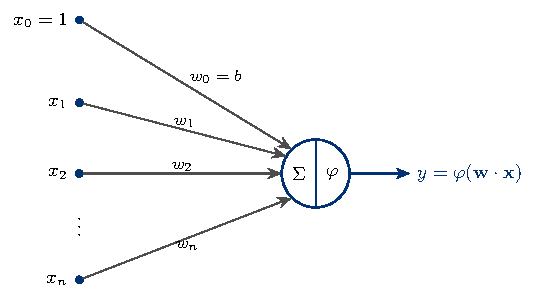
\includegraphics[height=4.0cm,width=5.1cm,keepaspectratio]{Fig13.pdf} &
      \centering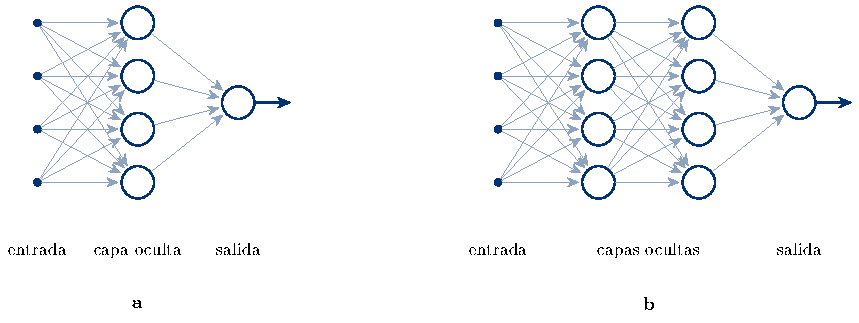
\includegraphics[height=4.0cm,width=5.1cm,keepaspectratio]{Fig27.pdf} &
      \centering\arraybackslash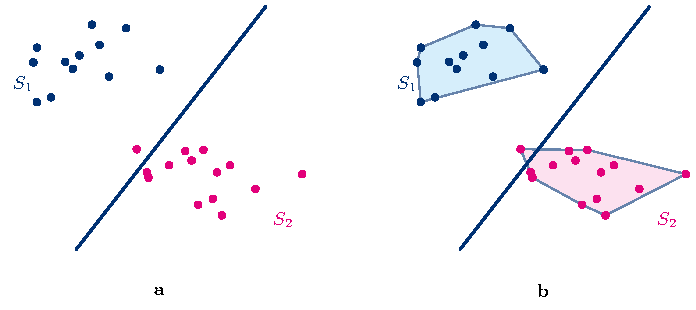
\includegraphics[height=4.0cm,width=5.1cm,keepaspectratio]{Fig37.pdf}\\[6pt]
      \centering{\small\color{icnavy}\textsc{Capítulo 5}\newline Neuronas abstractas}\par\vspace{2pt}
        {\scriptsize\color{icnavy!70}Una neurona: suma ponderada de las entradas y función de activación} &
      \centering{\small\color{icnavy}\textsc{Capítulo 6}\newline Redes neuronales}\par\vspace{2pt}
        {\scriptsize\color{icnavy!70}Neuronas organizadas en capas: la red con capas ocultas} &
      \centering\arraybackslash{\small\color{icnavy}\textsc{Capítulo 10}\newline Clasificación}\par\vspace{2pt}
        {\scriptsize\color{icnavy!70}Separabilidad lineal y convexa de clusters en el plano}
    \end{tabular}};
  % logos (si los archivos están disponibles)
  \IfFileExists{IC.jpeg}{\node[anchor=south] at ([xshift=-1.45cm,yshift=2.25cm]current page.south) {\includegraphics[height=1.9cm]{IC.jpeg}};}{}
  \IfFileExists{DM.png}{\node[anchor=south] at ([xshift=2.95cm,yshift=2.25cm]current page.south) {\includegraphics[height=1.9cm]{DM.png}};}{}
  \node[anchor=south,align=center,font=\small,text=icnavy!75] at ([xshift=0.75cm,yshift=1.15cm]current page.south)
    {Instituto de Cálculo, FCEN--CONICET \quad$\cdot$\quad Departamento de Matemática, FCEN--UBA};
\end{tikzpicture}
\null
\clearpage

%% REVERSO DE LA PORTADA
\thispagestyle{empty}
\null\vfill
\begin{flushleft}\small
Julián Fernández Bonder\\
Instituto de Cálculo, FCEN--CONICET\\
Departamento de Matemática, FCEN--UBA\\
Ciudad Universitaria, Pabellón 0+$\infty$ (1428), Buenos Aires, Argentina.\\[6pt]
{\it Correo:} \href{mailto:jfbonder@dm.uba.ar}{\texttt{jfbonder@dm.uba.ar}}\\
{\it URL:} \url{https://mate.dm.uba.ar/~jfbonder/}\\[12pt]
Notas del curso \emph{Fundamentos matemáticos del aprendizaje profundo}, optativa
del Departamento de Matemática, FCEN--UBA, 1er cuatrimestre de 2025.
Versión revisada en octubre de 2026.\\[12pt]
Estas notas son una traducción, con correcciones y aclaraciones, de partes del
libro de O.~Calin, \emph{Deep Learning Architectures}, Springer, 2020.
\end{flushleft}
\clearpage

\cleardoublepage
\chapter*{Prefacio}

Estas notas se escribieron para el curso optativo \emph{Fundamentos matemáticos
del aprendizaje profundo}, que dicté en el primer cuatrimestre de 2025 en el
Departamento de Matemática de la Facultad de Ciencias Exactas y Naturales de la
Universidad de Buenos Aires, con 21 clases. El curso busca presentar, como
conceptos matemáticos precisos, las ideas que en la práctica del aprendizaje
automático se usan de manera intuitiva: qué es una neurona, qué se puede
aprender con una red, y por qué.

\subsection*{Sobre la autoría}

Las notas son una traducción de la primera parte del libro de Calin~\cite{Calin},
al que sigue de cerca; no reclamo autoría sobre el contenido. Los Capítulos~1
a~9 corresponden a los Capítulos~1 a~9 del libro, y el Capítulo~10
(\emph{Clasificación}) al Capítulo~18. El Capítulo~10 del libro, sobre
aprendizaje exacto, no se incluye. En algunos lugares corregí o aclaré
demostraciones del libro; creo que eso puede tener algún valor didáctico, pero
recomiendo, para quien pueda, leer directamente el original.

\subsection*{Contenido y organización}

La primera parte (Capítulos~1 a~6) introduce las neuronas y las redes: los
problemas que motivan el concepto de neurona abstracta, las funciones de
activación y de costo, los algoritmos de minimización, y el cálculo del
gradiente en una red (la retropropagación). La segunda parte (Capítulos~7 a~10)
es de análisis: reúne las herramientas clásicas (Dini, Arzelà--Ascoli,
Stone--Weierstrass, el principio de contracción), las usa para demostrar que
las redes con una capa oculta aproximan funciones, y cierra con el problema de
clasificación. Cada capítulo comienza con un breve mapa de lo que contiene, y
termina con un resumen y una sección de ejercicios.

\subsection*{Convenciones}

Los vectores se escriben en negrita, $\xx,\ww$, y el producto interno es
$\ww\cdot\xx$. Una neurona calcula $y=\varphi(\ww\cdot\xx+b)$, donde $\ww$ son
los pesos, $b$ el sesgo y $\varphi$ la función de activación; $w_{ij}^{(\ell)}$
es el peso de la neurona $i$ de la capa $\ell-1$ a la neurona $j$ de la capa
$\ell$. El símbolo $\eta$ denota la tasa de aprendizaje. En los
Capítulos~1 a~6 el sesgo se absorbe en los pesos con una entrada
$x_0=1$ y $w_0=b$, de modo que $\ww\cdot\xx=\sum_{i=1}^n w_ix_i+b$. La letra $\varphi$ designa una función de activación general y $\sigma(x)=(1+e^{-x})^{-1}$ siempre es la función logística; $H$ es la función de Heaviside, con $H(0)=1$. En el Capítulo~9, para las redes que resuelven ecuaciones diferenciales, $\theta$ denota el vector de todos los parámetros.

\subsection*{Sobre la revisión}

Esta versión es una revisión de las notas originales, hecha en octubre de 2026
con la asistencia de herramientas de inteligencia artificial: corrige errores
y erratas, unifica la notación y mejora la presentación. La lista de cambios
está en el archivo \texttt{CAMBIOS.md} que acompaña a las notas. La
responsabilidad por los errores que hayan quedado es mía, y agradeceré que me
los señalen.

\bigskip
\noindent Buenos Aires, octubre de 2026.
\hfill Julián Fernández Bonder

\cleardoublepage
\tableofcontents 



\part{Introducción a las redes neuronales}

\chapter{Problemas introductorios}\label{cap1}

Empecemos discutiendo algunos problemas de la vida cotidiana que nos llevarán al concepto de {\em neurona abstracta} y {\em red neuronal}. Estos ejemplos, están basados en el problema de ajustar un cierto número de parámetros que detonan una cierta función de activación. Estos parámetros se ajustan para minimizar una {\em función de error}.

El capítulo parte de tres situaciones concretas: el llenado de un tanque de agua (Sección~\ref{sec.c1.1}), el problema de la regresión lineal (Sección~\ref{sec.c1.2}) y una red muy sencilla, la ``fábrica de cócteles'' (Sección~\ref{sec.c1.3}). En cada una hay parámetros que se ajustan para minimizar una función de error, y de ahí sale la idea de neurona abstracta. Corresponde al Capítulo~1 de~\cite{Calin}.

\section{Agua en un tanque}\label{sec.c1.1}

Una cañería lleva agua a una presión dada $P$ (ver la Figura \ref{fig1} {\bf a}). La canilla $K$ puede ajustar la presión del agua, produciendo una flujo variable a una tasa $r$. La canilla influencia la tasa introduciendo un control $w$ de manera tal que $P=r/w$.

Un cierto número de cañerías de este tipo son usadas para verter agua en un tanque (ver Figura \ref{fig1} {\bf b}). Simultáneamente, el tanque es drenado a una tasa $R$. El objetivo de este problema es: Dadas las presiones de agua $P_1,\dots, P_n$, cómo se pueden ajustar las canillas $K_1, \dots, K_n$ de manera tal que luego de un período de tiempo fijo $t$ haya un determinado volumen $V$ de agua en el tanque.
\begin{figure}[htbp]
\centering
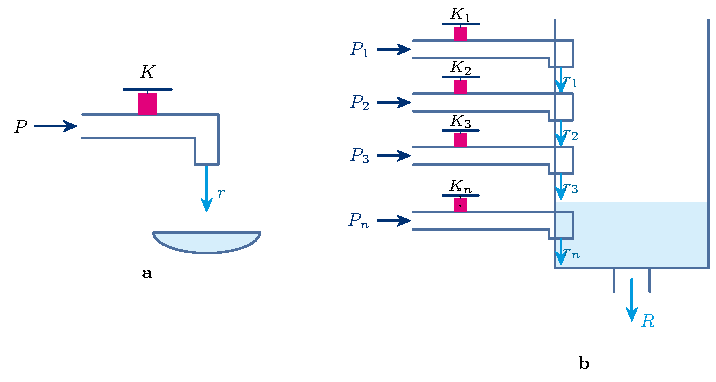
\includegraphics[max width=\linewidth]{Fig1.pdf}
\caption{{\bf a.} La canilla $K$ ajusta la presión $P$ en la cañería produciendo un flujo $r$. {\bf b.} Las $n$ canillas $K_1,\dots, K_n$ ajustan las presiones en las cañerías que vierten agua en el tanque con un desagüe teniendo un tasa de desagote $R$}
\label{fig1}
\end{figure}

Denotemos por $r_1,\dots, r_n$ a los flujos de agua ajustados por las canillas $K_1,\dots, K_n$. Si el flujo saliente $R$ excede la totalidad del flujo entrate (i.e. $R>\sum_{i=1}^n r_i$), entonces no se acumulará agua en el tanque (i.e. $V=0$). Caso contrario, si el total del flujo entrante es mayor que el saliente (i.e. $R<\sum_{i=1}^n r_i$), entonces el agua se acumulará en el tanque a una tasa igual a la diferencia de la tasa entrante y la saliente, con lo que la acumulación de agua sobre le intervalo de tiempo $t$ viene dado por $V = t\left(\sum_{i=1}^n r_i - R\right)$. Luego, la función que determina el volumen de agua total en el tanque luego de $t$ segundos, viene dado por la fórmula
$$
V=\begin{cases}
0, & \text{si } R>\sum_{i=1}^n r_i\\
t\left(\sum_{i=1}^n r_i - R\right), & \text{caso contrario.}
\end{cases}
$$
Podemos escribir esta función de manera equivalente. Si notamos $w_i$ al control provisto por la canilla $K_i$, entonces la $i-$ésima cañería provee agua a una tasa $r_i=P_i w_i$. Consideramos también la {\em función de activación}
$$
\varphi_t(x) = \begin{cases}
0, & \text{si } x<0\\
tx, & \text{caso contrario},
\end{cases}
$$
que depende del parámetro temporal $t>0$. Luego, el volumen de agua $V$ se puede escribir como
\begin{equation}\label{eq.ej.1}
V=\varphi_t\left(\sum_{i=1}^n P_i w_i + b\right).
\end{equation}
La tasa de salida $R$ produce una traslación horizontal al gráfico de $\varphi_t$ que en el lenguaje de las redes neuronales se denomina como {\em bias} o {\em sesgo}; en la fórmula aparece como $b=-R$. El problema se reduce entonces en encontrar una solución para la ecuación \eqref{eq.ej.1} teniendo como incógnitas $w_i$ y $b$. En la práctica alcanza con obtener una buena solución aproximada eligiendo para eso controles $w_i$ y el sesgo $b$ de manera tal que la {\em función de error}
$$
L(w_1,\dots,w_n,b) = \frac12 \left(\varphi_t\left(\sum_{i=1}^n P_i w_i + b\right) - V\right)^2
$$
sea minimizada. Otras funciones de error pueden ser utilizadas, como por ejemplo
$$
\tilde L(w_1,\dots,w_n,b) = \left|\varphi_t\left(\sum_{i=1}^n P_i w_i + b\right) - V\right|,
$$
pero esta presenta el inconveniente de que no es diferenciable.

En la práctica queremos aprender de los datos disponibles. Para eso disponemos de $N$ datos de entrenamiento que consisten en presiones $\Pb^k = (P_1^k,\dots,P_n^k)$ y volúmenes $V_k$, $1\le k\le N$. Usando estos datos, deberíamos poder pronosticar el volumen $V$ para cualquier otro vector de presiones $\Pb = (P_1,\dots,P_n)$.

Los controles $\ww=(w_1,\dots,w_n)$ se obtienen de los datos minimizando la función de costo
$$
C(\ww, b) = \frac12\sum_{k=1}^N (\varphi_t(\Pb^k\cdot\ww + b) - V_k)^2
$$
y para esos controles se realiza el pronóstico usando la fórmula \eqref{eq.ej.1}.


\section{Regresión lineal}\label{sec.c1.2}

Las redes neuronales no son un concepto reciente. Aparecieron por primera vez bajo el nombre de regresión lineal a principios del s. XIX en trabajos de Gauss y Legendre. Veamos como un modelo de regresión lineal puede ser naturalmente interpretado como una red neuronal.

Consideremos una función continua a valores reales $f\colon K\subset \R^n\to\R$ donde $K$ es un conjunto compacto. Queremos construir una función lineal $L=L(\xx)$ que aproxime $f$ en el sentido de $L^2$ usando una neurona con una activación lineal. La entrada es la variable $\xx=(x_1,\dots,x_n)\in K$ y la salida es la función lineal $L(\xx) = \sum_{j=1}^n a_j x_j + b$ donde $a_j$ son los pesos y $b$ es el sesgo de la neurona, ver la Figura \ref{fig2}.
\begin{figure}[htbp]
\centering
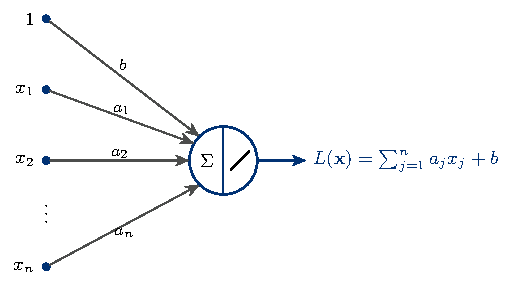
\includegraphics[max width=\linewidth]{Fig2.pdf}
\caption{Una neurona de aproximación lineal}
\label{fig2}
\end{figure}

Para simplificar el análisis, asumimos que la aproximación se realiza cerca del origen, i.e. $L(0)=f(0)$, lo que implica que el valor del sesgo es $b=f(0)$. Usando una traslación vertical, podemos siempre asumir que $f(0)=0$, con lo que podemos tomar el sesgo $b=0$. Luego, la función lineal es de la forma $L(\xx) = L_\ab(\xx) = \ab \cdot \xx$ donde $\ab = (a_1,\dots,a_n)$.

Consideramos como función de costo a la distancia $L^2$ entre la salida de la neurona y la función objetivo $f$,
$$
C(\ab) = \frac12 \int_K (L_\ab(\xx)-f(\xx))^2\, d\xx = \frac12 \int_K (\ab\cdot \xx - f(\xx))^2\, d\xx.
$$
Calculemos el gradiente de la función $C$.
\begin{align*}
\frac{\partial C}{\partial a_k}(\ab) &= \int_K x_k(\ab\cdot \xx - f(\xx))\, d\xx\\
& = \sum_{j=1}^n a_j \int_K x_j x_k\, d\xx - \int_K x_k f(\xx)\, d\xx\\
& = \sum_{j=1}^n a_j r_{jk} - m_k
\end{align*}
Luego,
$$
\nabla C(\ab) = R\ab^t - \mm^t,
$$
donde $R=(r_{jk})_{1\le j,k\le n}$ y $\mm=(m_1,\dots,m_n)$. Observemos que $R=R^t$.

El valor óptimo de los pesos $\ab=(a_1,\dots,a_n)$ se alcanzan entonces cuando $\nabla C(\ab)=0$. Si la matriz $R$ resulta inversible, entonce $\ab^t = R^{-1}\mm^t$.

En general el cálculo de $R^{-1}$ (sobre todo cuando la dimensión $n$ es grande) suele ser costoso computacionalmente y aún cuando la dimensión es pequeña, la matriz puede ser mal condicionada y su cálculo introducir errores significativos. Es mejor para eso utilizar otros métodos de resolución como por ejemplo el método de {\em descenso de gradiente}. Más adelante veremos con detalle este método.

Se toma un vector de pesos inicial $\ab_0$ y a partir de la misma se general la recursión
$$
\ab_{i+1} = \ab_i - \eta \nabla C(\ab_i),
$$
donde el parámetro $\eta>0$ se lo llama la {\em tasa de aprendizaje}. Se puede ver que esta sucesión $\{\ab_i\}_{i\ge 1}$ aproxima a la solución buscada.

Cuando se busca aproximar una función a valores vectoriales $F\colon K\subset \R^n\to \R^m$ con $m>1$, $F=(f_1,\dots, f_m)$, queremos hallar una función lineal del tipo $L(\xx)=A\xx^t + \bb^t$ donde ahora $A = (a_{jk})\in\R^{m\times n}$ es una matriz y $\bb=(b_1,\dots,b_m)\in \R^m$ es un vector de sesgo.

Nuevamente, si queremos aplicar la aproximación en $x=0$, sigue que el vector de sesgo $\bb=F(0)$ está fijo.  La salida de la $k-$ésima neurona estará dada por la $k-$ésima componente de $L$, $L_k(x)=\sum_{j=1}^n a_{jk}x_j + b_k$, ver la Figura 1.3.%\ref{fig3}.
\begin{figure}[htbp]
\centering
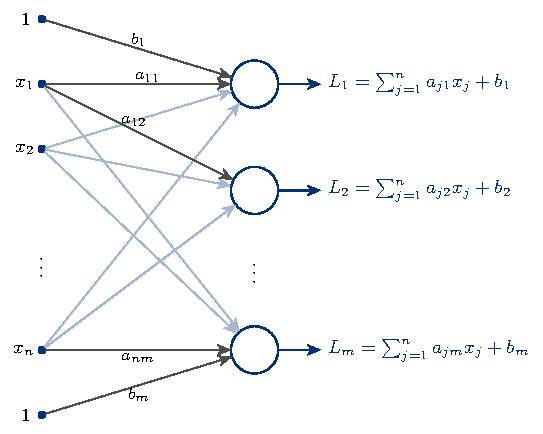
\includegraphics[max width=\linewidth]{Fig3.pdf}
\caption{Una red neuronal de aproximación lineal}
\label{fig3}
\end{figure}

La función de costo, será entonces
$$
C(A) = \frac12\int_K \|L(\xx)-F(\xx)\|^2\, d\xx = \sum_{k=1}^m C_k(\ab^k),
$$
donde $\ab^k=(a_{1k},\dots,a_{nk})$ es la $k-$ésima fila de la matriz $A$ y 
$$
C_k(\ab^k) = \frac12 \int_K (L_k(\xx) - f_k(\xx))^2\, d\xx = \frac12\int_K (\ab^k\cdot \xx + b_k - f_k(\xx))^2\, d\xx.
$$

La minimización del costo $C(A)$ es equivalente a la minimización simultánea de los costos $C_k(\ab^k)$, $1\le k\le m$. Cada uno de esas funciones de costo es relativa a una neurona y hemos mostrado su procedimiento de optimización en el caso escalar.

\section{La red de ``fábrica de cócteles''}\label{sec.c1.3}

En este ejemplo introduciremos la idea de la {\em red de aprendizaje profundo} que será el tópico central de este curso.

Asumamos que tenemos un flujo entrante de agua a una tasa $r$ en un tanque que tiene una canilla $K$ que controla el flujo saliente del tanque. Ver la Figura 1.4.%\ref{fig4}.
\begin{figure}[htbp]
\centering
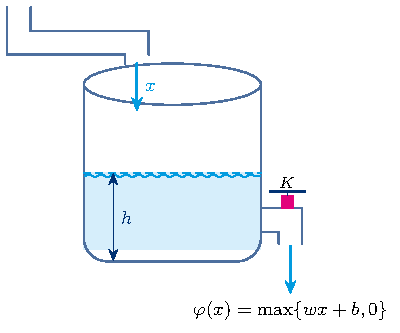
\includegraphics[max width=\linewidth]{Fig4.pdf}
\caption{Un tanque de agua con una canilla y un flujo saliente $\phi(x)=\max\{wx+b, 0\}$}
\label{fig4}
\end{figure}

La canilla está situada a una distancia $h$ del fondo del tanque. Luego de un cierto tiempo $t$, la cantidad de agua que fluyó dentro del tanque es $x=rt$. Notemos por $w$ al parámetro que controla el flujo saliente del tanque. Si $A$ es el área de la base del tanque, entonces $x-Ah$ representa el flujo sobrante y la cantidad $w(x-Ah) = wx+b$ sera eliminado del tanque por la canilla, donde $b=-wAh$. El flujo saliente del tanque se modela como
$$
\phi(x) = \max\{wx+b, 0\} = \begin{cases}
0, & \text{si } x\le -b/w\\
wx+b, & \text{caso contrario}.
\end{cases}
$$

Vamos ahora a organizar nuestros tanques en una red de seis tanques que mezclan tres ingredientes en un cóctel (ver la Figura 1.5). Azúcar, agua y vino se vierten en los tanques $A$, $B$ y $C$. Una mezcla de los tanques $A$ y $B$, se vierte al tanque $D$ como agua dulce y una mezcla de los tanques $B$ y $C$ se vierte al tanque $E$ como vino diluido. La mezcla producida por los contenidos de los tanques $D$ y $E$ se vierte al taque $F$. La canilla del tanque $F$ controla la producción final del cóctel.
\begin{figure}[htbp]
\centering
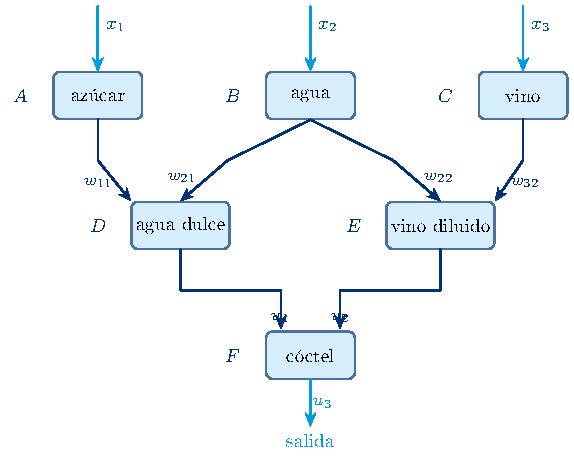
\includegraphics[max width=\linewidth]{Fig5.pdf}
\caption{Una fábrica de cócteles como una red neuronal con dos capas escondidas}
\label{fig5}
\end{figure}

La producción final del cóctel es le resultado de una combinación compleja de mezclas de los ingredientes, azúcar, agua y vino, vertidos en cantidades $x_1, x_2$ y $x_3$. Las canillas controlan la proporción de las soluciones que pasan al siguiente contenedor y son usadas para ajustar la calidad de la producción de cóctel. Luego de probar el resultado final, un experto en cóctel ajusta las canillas de manera tal que el cóctel mejore su calidad lo más posible. El proceso de ajuste de las canillas corresponde al aprendizaje de cómo hacer el cóctel de los ingredientes.


\section{Resumen}\label{sec.c1.4}

Veamos ahora como las características comunes de los ejemplos nos van a llevar a desarrollar nuevos conceptos abstractos como el perceptron y la red neuronal.

En todos los ejemplos se empieza con información entrante proporcionada por las variables $x_1,\dots,x_n$. En los ejemplos que vimos, estas son deterministas, pero podrían bien ser aleatorias (i.e. las mismas dependen de la observación realizada pero están distribuidas según una ley de probabilidad).

Otra característica en común es que los ingresos $x_i$ están multiplicados por un peso $w_i$ y luego esos productos están sumados formando expresiones del tipo $\sum_{i=1}^n w_i x_i$ que es el producto interno entre el vector de entradas $\xx=(x_1,\dots,x_n)$ y el vector de pesos $\ww = (w_1,\dots,w_n)$. En los ejemplos que vimos aparece sumando un sesgo $b$ (por ejemplo, $b=-R$ en el caso del umbral de la canilla). El mismo se puede eliminar introduciendo un nuevo peso $w_0=b$ y un nuevo ingreso $x_0=1$ lo que lleva a $\sum_{i=0}^n w_i x_i = \sum_{i=1}^n w_i x_i + b$ que también es el producto interno de dos vectores.

Otro ingrediente en común es la función de activación, denotada por $\varphi(x)$, Vimos algunos ejemplos de funciones de activación: lineales, lineales a trozos. Veremos de más tipos.

La función de salida $y$ se obtiene aplicando la función de activación $\varphi$ a el producto interno mediante la expresión $y=\varphi(\ww\cdot \xx)$. Si las variables de entrada $x_i$ son deterministas, la salida $y$ también lo será, pero si las entradas son variables aleatorias, la salida también será aleatoria.

El objetivo de estos ejemplos es el de ajustar el sistema de pesos $\ww$ de manera tal que la función de salida $y$ aproxime una cierta función de manera más precisa posible. En algunos casos, esto puede hacerse de manera exacta, pero en la mayoría será sólo una aproximación. Este objetivo se alcanza eligiendo los pesos $\ww$ de manera tal que cierta función de error sea minimizada. La función de error, es típicamente una función tipo distancia entre la salida realizada y la deseada. 

Resumiendo, en los ejemplos se tienen los siguientes ingredientes: entradas $\{x_i\}$, pesos $\{w_i\}$, sesgo $b$, una función de activación $\varphi(x)$ y una función de error. Estas partes son usadas para construir una función aproximante, mediante el proceso de ajustar los pesos que se lo denomina {\em aprendizaje} de los datos observados. Más adelante veremos un concepto abstracto que reúne todas estas propiedades y contiene todas estas características.

\section{Ejercicios}\label{sec.c1.5}

\begin{ejer}
Una fábrica tiene $n$ proveedores donde cada uno produce diferentes cantidades por día, $x_1,\dots,x_n$. La fábrica está conectada con sus proveedores por un sistema de rutas, que pueden ser utilizadas con capacidades variables $c_1,\dots,c_n$, de manera tal que la fábrica queda provista por una cantidad diaria $x=c_1 x_1 + \cdots + c_n x_n$.
\begin{itemize}
\item[(a)] Dado que la producción de la fábrica empieza cuando el suministro alcanza una cantidad crítica diaria $b$, escribir la fórmula para los ingresos diarios de la fábrica $y$.
\item[(b)] Formular el problema como un problema de aprendizaje.
\end{itemize}
\end{ejer}

\begin{ejer}
Un número $n$ de instituciones financieras, cada una teniendo una riqueza de $x_i$, deposita una cantidad de dinero en un fondo a una tasa ajustable para el depósito de $w_i$. Luego, el dinero en el fondo viene dado por $x=w_1 x_1 + \cdots + w_n x_n$. El fondo está diseñado para funcionar de la siguiente forma: mientras el fondo tenga menos que una cierta reserva $M$, el manager del fondo no realiza inversiones. Sólo se invierte el dinero excedente a la reserva $M$. Sea $k=e^{rt}$, donde $r$ y $t$ denotan la tasa de retorno y el tiempo de inversión respectivamente.
\begin{itemize}
\item[(a)] Hallar la fórmula para la inversión.
\item [(b)] Enunciar el problema de aprendizaje asociado.
\end{itemize}
\end{ejer}

\begin{ejer}
\begin{itemize}
\item[(a)] Dada una función continua $f\colon [0,1]\to \R$ hallar la función lineal $L(x)=ax+b$ tal que $L(0)=f(0)$ y que minimize el error cuadrático $\frac12 \int_0^1(L(x)-f(x))^2\, dx$.

\item[(b)] Dada una función continua $f\colon [0,1]\times [0,1]\to \R$ hallar la función lineal $L(x)=ax+by+c$ tal que $L(0,0)=f(0,0)$ y que minimize el error cuadrático 
$$\frac12 \int_0^1\int_0^1 (L(x,y)-f(x,y))^2\, dxdy.$$
\end{itemize}
\end{ejer}

\begin{ejer}
Dado un compacto $K\subset \R^n$, asociamos la matriz simétrica
$$
r_{ij} = \int_K x_i x_j\, dx.
$$
La inversibilidad de la matriz $R=(r_{ij})$ depende de $K$.
\begin{itemize}
\item[(a)] Probar que si $K$ tiene medida de Lebesgue positiva, entonces $R$ es inversible (para todo $n$). Mostrar que si $K$ tiene medida nula (por ejemplo, un segmento en $\R^2$), entonces $R$ no es inversible.
\item[(b)] Probar que si $K=[0,1]^n$, entonces $R$ es inversible para todo $n\ge 1$.
\end{itemize}
\end{ejer}

%%%%%%%%%%%%%%%%%%%%%%%%%%%%%%%%%%%%%%%%
%% CAPITULO 2 %%%%%%%%%%%%%%%%%%%%%%%%%%%%%%%
%%%%%%%%%%%%%%%%%%%%%%%%%%%%%%%%%%%%%%%%

\chapter{Funciones de activación}\label{cap2}

Para poder aprender una función no lineal objetivo, una red neuronal usa funciones de activación que son no lineales. La elección de una función de activación específica define tipos diferentes de redes neuronales. Dentro de la enorme variedad de funciones de activación que existen en la literatura, los tipos más comúnmente usados son: funciones lineales, funciones escalón, funciones sigmoidales y funciones {\em palo de hockey}; también se usan funciones {\em sombrero}.

Cada una de estas funciones tiene ventajas y desventajas (continuidad, diferenciabilidad, acotación, etc.) que aparecen a la hora de realizar diferentes cálculos.

El capítulo presenta las funciones de activación que usaremos a lo largo del curso (Sección~\ref{sec.c2.1}) y las propiedades que importan para el entrenamiento. La sección final las resume. Corresponde al Capítulo~2 de~\cite{Calin}.

\section{Algunos ejemplos de funciones de activación}\label{sec.c2.1}

\subsection*{Funciones lineales} La pendiente de la función lineal puede ser usada para modelar la tasa de activación de una neurona. Se suele usar fundamentalmente en una red de multicapa para la capa de salida. Una neurona con una función de activación lineal es equivalente a una regresión lineal: $f(x)=kx$.

\subsection*{Funciones escalón} Este tipo de función de activación está inspirado en neuronas biológicas que exhiben saltos que simplificadamente modelan la activación de una neurona del sistema nervioso. Los ejemplos más comunes son:
\subsubsection*{Función de Heaviside} Está dada por
$$
H(x)=\begin{cases}
0, &\text{si } x<0\\
1, &\text{si } x\ge 0.
\end{cases}
$$
Si bien esta función no es diferenciable en el origen, si tiene derivada en sentido de distribuciones, $H'=\delta$, donde $\delta$ es la {\em delta de Dirac}. Recordemos que $\delta$ no es una función sino la distribución definida por
$$
\int_\R \delta(x)\,\varphi(x)\, dx = \varphi(0)\qquad\text{para toda } \varphi\in C_c^\infty(\R).
$$
En efecto, $\int_\R H\,\varphi'\,dx=\int_0^\infty\varphi'\,dx=-\varphi(0)$. (La descripción heurística ``vale $0$ si $x\neq0$ y $+\infty$ si $x=0$, con integral $1$'' es útil como intuición, pero no define nada: una función que vale $0$ salvo en un punto tiene integral $0$.) Para $x\neq0$, $H$ es derivable y $H'(x)=0$.

\subsubsection*{Función bipolar} A veces se la llama (con algo de abuso) función signo; se define como
$$
S(x)=\begin{cases}
-1, &\text{si } x<0\\
1, &\text{si } x\ge 0.
\end{cases}
$$
Se ve fácilmente que se tiene la relación $S(x) = 2H(x)-1$ y en consecuencia $S'=2\delta$ en el sentido de distribuciones. Notemos que $S(0)=1$, mientras que la función signo usual cumple $\operatorname{sgn}(0)=0$; coinciden para $x\ne0$.

\subsection*{Funciones palo-de-hockey} Estas son funciones cuyos gráficos son similares a los de un palo de hockey. Algunos ejemplos:
\subsubsection*{Unidad lineal rectificada (ReLU)} En este caso, la activación es lineal sólo si $x\ge 0$.
$$
\text{ReLU}(x) = x H(x)=\max\{0,x\} = \begin{cases} 0, &\text{si } x<0\\ x, & \text{caso contrario.}\end{cases}
$$
La ReLU no es derivable en $x=0$; para $x\neq0$ se tiene $\text{ReLU}'(x) = H(x)$, y en sentido distribucional $\text{ReLU}'=H$. En la práctica se adopta una convención para el valor de la derivada en $0$ (habitualmente $0$ o $1$), que no influye porque el conjunto $\{0\}$ tiene medida nula.

\subsubsection*{Unidad lineal rectificada paramétrica (PReLU)} En este caso la activación es lineal a trozos con distinta pendiente si $x<0$ o $x\ge 0$.
$$
\text{PReLU}(\alpha, x) = \begin{cases} \alpha x, &\text{si } x<0\\ x, & \text{caso contrario.}\end{cases}
$$

\subsubsection*{Unidad lineal exponencial (ELU)} Esta función es lineal y positiva para $x>0$ y negativa exponencial para $x<0$.
$$
\text{ELU}(\alpha, x) = \begin{cases}  x, &\text{si } x>0\\ \alpha(e^x-1), & \text{si } x\le 0\end{cases}
$$
Esta función es diferenciable en $x=0$ si y sólo si $\alpha=1$.

\subsubsection*{Unidad lineal sigmoidal (SiLU o Swish)} Buscamos una función suave ($C^\infty$) con el mismo comportamiento de ``palo de hockey'' que la ReLU. Eso podemos obtenerlo de la forma
$$
\text{SiLU}(x) = x\sigma(x) = \frac{x}{1+e^{-x}}. 
$$
Observemos que esta función es aproximadamente lineal para $x\gg 1$ (pues $\sigma(x)\to1$) y que $\text{SiLU}(x)\to0^-$ para $x\to-\infty$ (pues $|x|e^{x}\to0$). Sin embargo no es monótona: tiene un único mínimo global, de valor aproximado $-0{,}278$, en $x\approx-1{,}278$, y es negativa para $x<0$. A diferencia de la ELU, que tiende a $-\alpha$, la SiLU tiende a $0$ en $-\infty$.

\subsection*{Funciones sigmoidales} Este tipo de funciones de activación tienen la ventaja de ser suaves y que pueden aproximar a las funciones escalón con la precisión deseada. Cuando se normalizan para que sus valores estén en $[0,1]$ su valor puede interpretarse como una probabilidad. Algunos ejemplos:

\subsubsection*{Función logística}
$$
\sigma_c(x) = \sigma(c,x) = \frac{1}{1+e^{-cx}},
$$
donde el parámetro $c>0$ controla la tasa de encendido de la neurona en el sentido de que valores grandes de $c$ corresponden a cambios rápidos de 0 a 1.

Observemos que cuando $c\to\infty$, tenemos que $\sigma(c,x)\to H(x)$ para $x\neq 0$.

\subsubsection*{Tangente hiperbólica} También se la llama función sigmoidal bipolar.
$$
\tb(x) = \tanh x = \frac{e^x - e^{-x}}{e^x + e^{-x}}.
$$
Se relaciona con la logística por $\tanh x=2\sigma(2x)-1$, de modo que toma valores en $(-1,1)$ y $\tanh'(x)=1-\tanh^2(x)\in(0,1]$.

\subsubsection*{Softplus} Es una versión suave de la ReLU:
$$
\text{softplus}(x)=\ln(1+e^{x}),
$$
que es $C^\infty$, estrictamente creciente y convexa, con $\text{softplus}'=\sigma$ y $\text{softplus}(x)-\text{ReLU}(x)\to0$ para $|x|\to\infty$. La usaremos en el Capítulo~\ref{cap8}.

\subsection*{Funciones sombrero} Estas funciones de activación se utilizan cuando la neurona es activada al máximo para un cierto valor del potencial de acción.

\subsubsection*{Gaussiana} 
$$
g(x) = e^{-x^2}
$$

\subsubsection*{Doble exponencial} 
$$
f(x) = e^{-\lambda |x|},\quad \lambda>0.
$$


\section{Resumen}\label{sec.c2.2}
Cada unidad en una red neuronal usa una función que procesa la señal entrante, llamada la función de activación. La importancia de estas funciones de activación es la de introducir no-linealidades en la red. Activaciones lineales sólo pueden producir resultados lineales y sólo pueden ser utilizadas para una clasificación lineal (o problemas de regresión lineal), lo que resulta muy restrictivo. Las funciones de activación no lineales resuelven este problema.

Existen muchos tipos diferentes de funciones de activación que han sido propuestos en la literatura cada una de ellas para un propósito diferente. Algunas de las mismas las hemos visto en este capítulo.


\section{Ejercicios}\label{sec.c2.3}
\begin{ejer}
\begin{itemize}
\item[(a)] Mostrar que la función logística $\sigma(x)$ verifica la desigualdad $0<\sigma'(x)\le \frac14$ para $x\in\R$.

\item[(b)] ¿Cómo se modifica esa desigualdad para la función $\sigma_c(x)$?
\end{itemize}
\end{ejer}

\begin{ejer}
Sean $S(x)$ y $H(x)$ las funciones signo y Heaviside respectivamente. Mostrar que
\begin{itemize}
\item[(a)] $S(x)=2H(x) - 1$,

\item[(b)] $\text{ReLU}(x) = \frac12 x(S(x)+1)$.
\end{itemize}
\end{ejer}


%%%%%%%%%%%%%%%%%%%%%%%%%%%%%%%%%%%%%%%%
%% CAPITULO 3 %%%%%%%%%%%%%%%%%%%%%%%%%%%%%%%
%%%%%%%%%%%%%%%%%%%%%%%%%%%%%%%%%%%%%%%%

\chapter{Funciones de costo}\label{cap3}

En el proceso de aprendizaje, los parámetros de una red neuronal se deben ajustar para minimizar ciertas funciones objetivo que representan la medida de la proximidad entre lo que predice la red y el objetivo buscado. Esto es conocido con los nombres equivalentes de {\em funciones de costo}, {\em funciones de pérdida} o {\em funciones de error}. En este capítulo vamos a describir las funciones de costo más usuales en redes neuronales.


Este capítulo define qué se le pide a una red: la entrada, la salida y el objetivo (Sección~\ref{sec.c3.1}), los principales ejemplos de función de costo (Sección~\ref{sec.c3.2}) y su combinación con términos de regularización (Sección~\ref{sec.c3.3}). Luego se distingue el error de entrenamiento del de test (Sección~\ref{sec.c3.4}), y se da una interpretación geométrica del problema con restricciones (Sección~\ref{sec.c3.5}). Corresponde al Capítulo~3 de~\cite{Calin}.

\section{Entrada, salida y objetivo}\label{sec.c3.1}

La entrada de una red neuronal es obtenida de datos conocidos o de sensores que perciben el entorno. La entrada es la variable con la que se alimenta la red. Puede ser una variable unidimensional $x\in\R$, un vector $\xx\in \R^n$, una matriz, o una variable aleatoria $X$.

La red en sí actúa como una función, es decir, modifica la variable de entrada de una cierta manera y produce una salida que puede ser, nuevamente, unidimensional $y\in\R$, un vector $\yy\in \R^m$, una variable aleatoria $Y$, etc. La ley por la cual la entrada es modificada en la salida se realiza mediante un {\em mapeo ingreso-egreso}, $f_{w,b}$. El índice $(w, b)$ sugiere que los parámetros internos de la red mientras se realiza esta asignación están fijados en $(w, b)$. Siguiendo las notaciones previas, tendríamos $y=f_{w, b}(x)$, o $\yy = f_{w, b}(\xx)$, o $Y=f_{w, b}(X)$.

La {\em función objetivo} es la relación deseada que la red trata de aproximar. Esta función es independiente de los parámetros $(w, b)$ y será denotada, según corresponda, por $z=\phi(x)$, o $\zz = \phi(\xx)$, o $Z=\phi(X)$, según los datos sean unidimensionales, vectoriales o variables aleatorias. Podría eventualmente, haber alguna mezcla, por ejemplo $z=\phi(\xx)$ cuando la entrada sea vectorial, pero la salida unidimensional.

La red neuronal, ajusta los parámetros $(w, b)$ hasta que la variable de salida $y$ se encuentre dentro de un entorno de la variable objetivo $z$. Esta proximidad se puede medir de diferentes maneras, involucrando diferentes funciones de costo, $C(w, b)=\text{dist}(y, z)$, con una distancia a ser determinada. Los valores óptimos de los parámetros de la red serán dados por $(w^*, b^*)=\argmin_{(w, b)} C(w, b)$.

El proceso por el cual los parámetros $(w, b)$ se van ajustando a $(w^*, b^*)$ se lo llama {\em aprendizaje}. Equivalentemente, decimos que la red aprende la función objetivo $\phi(x)$. Este proceso de aprendizaje involucra la minimización de la función costo. En este capítulo vamos a investigar algunos tipos de función costo.


\section{Ejemplos de función costo}\label{sec.c3.2}

Vamos a ver algunos ejemplos, pueden consultar otros adicionales en el libro \cite{Calin}.
 
\subsection{Función de error de supremo}
Asumamos que la red neuronal, que toma valores de entrada $x\in [0,1]$, debe aprender una función continua $\phi\colon [0,1]\to \R$. Si $f_{w, b}$ es el mapa entrada-salida de la red, entonces la función costo supremo asociada es
$$
C(w, b) = \sup_{x\in [0,1]} |f_{w, b}(x) - \phi(x)|.
$$
A todo uso práctico, la función objetivo es conocida en finitos puntos
$$
z_i = \phi(x_i),\qquad 1\le i\le n,
$$
luego la función costo usada es
$$
C(w, b) = \max_{1\le i\le n}  |f_{w, b}(x_i) - z_i|.
$$

\subsection{Función de error $L^2$}\label{L2}
Como en el caso anterior, supongamos que la variable de entrada es $x\in [0,1]$ y la función objetivo es $\phi\colon [0,1]\to \R$. Si $f_{w, b}$ es el mapa entrada-salida de la red, la función costo que mide la distancia $L^2$ entre la salida y el objetivo es
$$
C(w, b) = \int_0^1 (f_{w, b}(x) - \phi(x))^2\, dx.
$$
Nuevamente, si se conoce la función objetivo sólo en $n$ puntos,
$$
z_i = \phi(x_i),\qquad 1\le i\le n,
$$
entonces la función costo es la distancia Euclideana en $\R^n$
 $$
 C(w, b) = \sum_{i=1}^n (f_{w, b}(x_i) - z_i)^2 = \| f_{w, b}(\xx) - \zz\|^2,
 $$
 donde $\xx=(x_1,\dots,x_n)$, $\zz = (z_1,\dots,z_n)$ y $f_{w, b}(\xx) = (f_{w, b}(x_1),\dots,f_{w, b}(x_n))$. Según el contexto, estas funciones de costo se normalizan con un factor $\frac12$ o $\frac1n$; esto no cambia los minimizadores.

Observemos que para $\xx, \zz\in \R^n$ fijos, $C(w, b)$ es una función suave y la misma puede ser minimizada, por ejemplo, por el método de descenso de gradiente que estudiaremos en el siguiente capítulo.

\subsection{Función de error cuadrático medio}
Consideremos ahora una red neuronal cuya entrada es una variable aleatoria $X$, y su salida es la variable aleatoria $Y=f_{w, b}(X)$, donde $f_{w, b}$ es el mapa de entrada-salida de la red. Asumamos que la red es usada para aproximar a la variable aleatoria objetivo $Z$. 

La función de error en este caso, mide la proximidad de la salida $Y$ con el objetivo $Z$. Una forma habitual de medir esa proximidad es mediante la esperanza de la diferencia al cuadrado
$$
C(w, b) = \E[(Y-Z)^2] = \E[(f_{w, b}(X)-Z)^2].
$$
Para hallar el mínimo $(w^*, b^*) = \argmin C(w, b)$ se utiliza alguno de los algoritmos de minimización que veremos en el capítulo siguiente.

Veamos algunas de las razones de por qué esta función de error (y la vista en la sección \ref{L2}) son muy utilizadas.
\begin{enumerate}
\item Las variables aleatorias de cuadrado integrable sobre un espacio de probabilidad forman un {\em espacio de Hilbert} con producto interno dado por $\langle X, Y\rangle = \E[XY]$. Esto define una norma $\|X\|^2 = \E[X^2]$ la cual induce una distancia $\dist(X, Y) = \|X-Y\|$.

Luego, la función costo no es otra cosa que el cuadrado de la distancia $C(w, b) = \dist(Y, Z)^2$.

\item Otro motivo es la relación que existe entre la función de costo y la esperanza condicional. La red neuronal transforma a la variable aleatoria de entrada en otra de salida $Y=f_{w, b}(X)$ que es parametrizada por $w$ y $b$. La información generada por la variable aleatoria $f_{w, b}(X)$ es la $\sigma-$álgebra ${\mathcal E}_{w, b} = \sigma(f_{w, b}(X))$ (es decir, la menor $\sigma-$álgebra que hace medible a $f_{w, b}(X)$). Todas estas $\sigma-$álgebras generan toda la información de salida ${\mathcal E} = \bigvee_{w, b} {\mathcal E}_{w, b}$ que es la $\sigma-$álgebra generada por la unión $\bigcup_{w, b} {\mathcal E}_{w, b}$. (La notación ${\mathcal E}$ viene de {\em exit}, salida en inglés).

En general, la variable aleatoria objetivo $Z$ (que supondremos de cuadrado integrable) no está determinada por la información $\mathcal E$. El problema entonces puede formularse como: {\em dada la información de salida $\mathcal E$, hallar la mejor aproximación de $Z$ basada en la información $\mathcal E$}. Esta es la variable aleatoria $\hat Z=\E[Z|{\mathcal E}]$, que se llama la {\em esperanza condicional} de $Z$ dado $\mathcal E$. Es $\mathcal E-$medible y minimiza la distancia a $Z$ entre todas las variables aleatorias $U$ de cuadrado integrable que son $\mathcal E-$medibles:
$$
\dist(\hat Z, Z) = \min_{U,\ {\mathcal E}-\text{medible}} \dist(U,Z).
$$
Es decir, $\hat Z$ es la proyección ortogonal de $Z$ sobre el subespacio de las variables $\mathcal E-$medibles de cuadrado integrable (con respecto al producto interno $\langle X, Y\rangle = \E[XY]$). Como cada salida $f_{w,b}(X)$ es $\mathcal E-$medible, para todo $(w,b)$ vale
$$
C(w,b)\ \ge\ \E[(\hat Z-Z)^2].
$$
Esta es una cota inferior ideal para el costo. Se alcanza solamente si $\hat Z$ pertenece a la familia $\{f_{w,b}(X)\}_{w,b}$, lo que en general no ocurre, porque la red no produce todas las variables $\mathcal E-$medibles.

\item La definición de función de costo puede extenderse fácilmente al caso en el que las variables aleatorias son conocidas por mediciones. Consideremos $n$ mediciones de las variables aleatorias $(X, Z)$ dadas por $(x_1, z_1),\dots,(x_n,z_n)$. Esto forma lo que se denomina como el {\em conjunto de entrenamiento} de la red neuronal. Entonces, en este caso la función de costo se define como 
$$
\tilde C(w, b) = \frac{1}{n}\sum_{i=1}^n (f_{w, b}(x_i)-z_i)^2,
$$
que es la media empírica del cuadrado de la diferencia entre $Y$ y $Z$.
\end{enumerate}

Observemos que en el caso trivial en el que las variables $X$ y $Z$ son independientes, la red neuronal es poco lo que puede hacer. En efecto, si $X$ y $Z$ son independientes, entonces también lo serán $f_{w, b}(X)$ y $Z$ con lo que la información de salida $\mathcal E$ va a ser independiente de $Z$. En consecuencia, nuestro mejor estimador será
$$
\hat Z=\E[Z|\mathcal E] = \E[Z].
$$
Es decir que el mejor estimador es simplemente un número que es el promedio de mis mediciones.

\subsection{Entropía cruzada}

Vamos a presentar la definición y propiedades de la entropía cruzada para el caso unidimensional. Más adelante lo usaremos en el caso de dimensión 2. 

Sean $p$ y $q$ dos densidades en $\R$. Se define la {\em log-verosimilitud negativa} de $q$ como 
$$
-\ell_q(x) = -\ln q(x).
$$
Esta función mide la información proporcionada por $q(x)$. Observemos que si $q(x)$ es grande, quiere decir que estamos en regiones de alta probabilidad con lo que no tenemos mayor detalle de lo que ocurre y en ese caso $-\ell_q(x)$ es pequeño (para una probabilidad discreta, cercano a $0$). Mientras que si $q(x)\sim 0$, estamos en regiones de baja probabilidad, con lo que ese dato nos da información mucho más precisa y $-\ell_q(x)\gg 1$.

La función de entropía cruzada de $p$ con respecto a $q$ se define como la esperanza con respecto a $p$ de la función de verosimilitud negativa de $q$, es decir
$$
S(p, q) = \E^p[-\ell_q] = -\int_\R p(x)\ln q(x)\, dx.
$$
Esta función mide la información proporcionada por $q$ desde el punto de vista de la distribución $p$ que se supone conocida. Para probabilidades discretas (con la suma en lugar de la integral), como $q\in (0,1]$ se tiene $-\ln q\ge0$ y por lo tanto $S(p, q)\ge 0$. Sin embargo tenemos un resultado más fino:
\begin{prop}\label{cota.entropia}
Se tiene la desigualdad $S(p, q)\ge H(p)$ (si $H(p)$ es finita; en general, lo que se prueba es $\int p\ln(p/q)\ge 0$), donde $H(p)$ es la {\em entropía de Shannon} definida como
$$
H(p) = S(p, p) = -\E^p[\ell_p] = -\int_\R p(x)\ln p(x)\, dx.
$$
\end{prop}

\begin{proof}
Usamos la convención $0\ln0=0$ y llamamos $A=\{p>0\}$. Entonces
\begin{align*}
S(p, q) - H(p) &= -\int_A p(x)\ln \frac{q(x)}{p(x)}\, dx
\end{align*}
(el integrando solo importa donde $p>0$). Ahora usamos la desigualdad elemental $\ln t \le t-1$ para $t>0$, es decir, $-\ln t\ge 1-t$, y obtenemos
\begin{align*}
S(p, q) - H(p) &\ge \int_A p(x) \left(1-\frac{q(x)}{p(x)}\right)\, dx
= \int_A p(x)\, dx - \int_A q(x)\, dx = 1 - \int_A q(x)\, dx\ \ge\ 0,
\end{align*}
porque $\int_A q\le\int_\R q=1$. Luego $S(p, q)-H(p)\ge 0$.

Si hay igualdad, entonces las dos desigualdades anteriores son igualdades. Como $\ln t<t-1$ para $t\neq1$, la primera obliga a que $q=p$ en casi todo punto de $A$; y la segunda a que $\int_A q=1$, es decir, que $q=0$ en casi todo punto fuera de $A$. Como $p=0$ fuera de $A$, resulta $p=q$ en casi todo punto. La recíproca es inmediata.
\end{proof}

Este resultado nos dice que dada una densidad $p$, el mínimo de la entropía cruzada $S(p, q)$ se alcanza cuando $q=p$ y ese mínimo coincide con la entropía de Shannon de la densidad $p$. La diferencia $S(p,q)-H(p)=\int p\ln(p/q)$ se llama {\em divergencia de Kullback--Leibler} de $p$ respecto de $q$.

Observemos que en el caso de densidades continuas, la entropía $H(p)$ puede ser finita (positiva o negativa) o bien puede ser infinita, pero si $p$ es una probabilidad discreta, entonces $H(p)\ge0$ (con $H(p)=0$ si y solo si $p$ es una delta); es finita si el soporte es finito, pero puede ser $+\infty$ si el soporte es infinito numerable.

Para densidades continuas con esperanza y varianza finitas, la entropía de Shannon está acotada superiormente (aunque, en general, puede valer $-\infty$):
\begin{cor}
Sea $X$ una variable aleatoria sobre $\R$ con densidad $p$. Asumimos que $X$ tiene esperanza y varianza finita. Entonces
$$
H(p)\le \frac12 \ln(2\pi e \V(X)),
$$
donde $\V(X) = \E[(X-\E[X])^2]$ es la varianza.
\end{cor}

\begin{proof}
Llamemos $\mu = \E[X]$ y $\sigma^2 = \V[X]$. Definamos ahora la densidad normal $q$ con misma esperanza y varianza que $p$, es decir, $q(x) = \frac{1}{\sqrt{2\pi\sigma^2}} e^{-\frac{(x-\mu)^2}{2\sigma^2}}$. Observemos entonces que por la Proposición \ref{cota.entropia} se tiene que
$$
H(p)\le S(p, q).
$$
Ahora, la entropía cruzada de $p$ con respecto a $q$ se puede calcular explícitamente:
\begin{align*}
S(p, q) &= - \int_\R p(x)\ln q(x)\, dx = \frac12 \ln(2\pi\sigma^2) + \frac{1}{2\sigma^2}\int_\R p(x) (x-\mu)^2\, dx\\
&= \frac12 \ln(2\pi\sigma^2) + \frac12 = \frac12 \ln(2\pi e\sigma^2),
\end{align*}
usando que $\int_\R p(x)(x-\mu)^2dx=\sigma^2$. Luego $H(p)\le\frac12\ln(2\pi e\sigma^2)$.
Esto finaliza la demostración. Observemos que la igualdad se alcanza para variables aleatorias normalmente distribuidas.
\end{proof}

\begin{obs}
La entropía cruzada se utiliza por lo general en problemas de clasificación, mientras que el error cuadrático medio es usado en problemas de regresión.
\end{obs}

\section{Funciones de costo y regularización}\label{sec.c3.3}

Para evitar los problemas de sobreajuste de los datos de entrenamiento (overfitting), es conveniente agregar términos adicionales a las funciones de costo. Se puede observar que el modelo suele sobreajustar los datos de entrenamiento si se permite que los parámetros tomen valores arbitrariamente grandes. Sin embargo, si se restringen los valores de los parámetros a permanecer acotados, esto impide que el modelo pase por todos los puntos de entrenamiento y por ende previene el sobreajuste. 

Para lograr esta restricción, se suelen usar términos de regularización a las funciones de costo. Los términos más usuales son tipo $L^1$ o $L^2$.

\subsubsection*{Regularización $L^2$} Consideremos los parámetros $\ww\in\R^n$. Su norma euclídea (o $\ell^2$) es $\|\ww\|_2=\bigl(\sum_{i=1}^n w_i^2\bigr)^{1/2}$, de modo que $\|\ww\|_2^2 = \sum_{i=1}^n w_i^2$. La función de costo con la regularización $L^2$ se obtiene sumando un múltiplo del cuadrado de la norma a la función de costo original
$$
C^{(2)}_\lambda(\ww) = C(\ww) + \lambda \|\ww\|_2^2,
$$
donde $\lambda>0$ es un hiperparámetro (que en la Sección~\ref{sec.c3.5} se interpretará como un multiplicador de Lagrange) que regula el equilibrio entre el tamaño de los pesos y el mínimo de $C(\ww)$. Un valor grande de $\lambda$ significa un valor pequeño de los pesos a costa de un valor grande para $C(\ww)$. Análogamente, un valor pequeño de $\lambda$ permite valores grandes de los pesos y un valor más pequeño del costo, con el riesgo de que el modelo sobreajuste. El valor del {\em hiperparámetro} $\lambda$ debe ser seleccionado para conseguir minimizar el sobreajuste sin aumentar demasiado el costo.

\subsubsection*{Regularización $L^1$} La norma $L^1$ de $\ww\in\R^n$ se define como $\|\ww\|_1 = \sum_{i=1}^n |w_i|$. Luego, la función costo con regularización $L^1$ se define como
$$
C^{(1)}_\lambda(\ww) = C(\ww) + \lambda \|\ww\|_1.
$$
El rol del hiperparámetro $\lambda$ es similar al caso $L^2$. Observemos que la norma $L^1$ no es diferenciable con lo que algunos métodos de minimización pueden no funcionar adecuadamente. A cambio, la regularización $L^1$ favorece soluciones {\em ralas}, con muchos pesos exactamente nulos, y ese es el principal motivo para usarla.

\subsubsection*{Regularización potencial} Esta es una generalización de las dos regularizaciones previas. Se considera una función $U\colon \R^n\to[0,\infty)$ tal que $U(\xx)=0$ si y sólo si $\xx=0$ (en particular, $U$ tiene un mínimo global en $0$). En el caso en que $U$ sea de clase $C^2$, esto implica necesariamente que $\nabla U(0)=0$ y $D^2U(0)\ge 0$. La función $U$, llamada {\em función potencial}, es una generalización de las normas $L^1$ y $L^2$.

La función de costo regularizada se define entonces como
$$
G(\ww) = C(\ww) + \lambda U(\ww),\qquad \lambda>0.
$$

La elección del potencial óptimo que posea las mejores propiedades de regularización para una función de costo dada, se realiza verificando su performance en el conjunto de validación (ver la sección siguiente). El error de validación debe decrecer significativamente cuando el término $U(\ww)$ es agregado a la función de costo inicial $C(\ww)$.

\section{Entrenamiento y test de errores}\label{sec.c3.4}

Una de las principales características que hace diferente el aprendizaje automático (machine learning) a un problema regular de optimización, que minimiza sólo un error, es el problema de doble optimización con dos tipos diferentes de errores que serán discutidos en esta sección. Es la diferencia entre estos dos errores lo que determinará qué tan bien funciona el algoritmo de aprendizaje automático.

En un enfoque basado en aprendizaje automático el conjunto de datos $\{(x_i, z_i)\}_{i\in I}$ es dividido en tres partes: {\em conjunto de entrenamiento}, {\em conjunto de testeo} y {\em conjunto de validación}. Se asume que todos estos conjuntos poseen idéntica distribución, siendo generados por una distribución de probabilidad en común. Otra hipótesis es que cada uno de estos conjuntos de datos son independientes entre sí. En cuanto a los tamaños, el más grande de estos conjuntos de datos es el de entrenamiento $\Tc$ que suele tener aproximadamente el $70\%$ de los datos. El segundo es el de testeo $T$ que tiene aproximadamente el $20\%$ de los datos. Finalmente el de validación $\Vc$ con aproximadamente el $10\%$.

La función de costo evaluada en los datos del conjunto de entrenamiento se llama el {\em error de entrenamiento}. Similarmente, la función de costo evaluada en los datos del conjunto de testeo se llama {\em error de testeo} o {\em error de generalización}. Por ejemplo,
\begin{align*}
& C_{\Tc}(w, b) = \frac{1}{m}\sum_{j=1}^m (f_{w, b}(x_j)-z_j)^2,\qquad (x_j, z_j)\in \Tc\\
& C_T(w, b) = \frac{1}{k}\sum_{i=1}^k (f_{w, b}(x_i)-z_i)^2,\qquad (x_i, z_i)\in T,
\end{align*}
con $m=\#\Tc$ y $k=\# T$, son los errores de entrenamiento y de testeo respectivamente asociados al promedio de la suma de los cuadrados.

En una primera etapa, un proceso de optimización (como el método de descenso de gradiente) es usado para minimizar el error de entrenamiento $C_\Tc(w, b)$ ajustando los parámetros $(w, b)$. Notemos por $(w^*, b^*)$ los valores óptimos de los parámetros. Este procedimiento se llama {\em entrenamiento}.

En una segunda etapa evaluamos el error de testeo en los valores optimales de los parámetros que hayamos, obteniendo un error de testeo $C_T(w^*, b^*)$. En general, se espera obtener la desigualdad
$$
C_\Tc(w^*, b^*)\le C_T(w^*, b^*).
$$
Las siguientes variantes son posibles:
\begin{enumerate}
\item Ambos errores, $C_\Tc(w^*, b^*)$ y $C_T(w^*, b^*)$, son pequeños. Esto significa que la red generaliza bien, es decir que no sólo responde bien en el conjunto de entrenamiento, sino que también en datos no usados. Este es el escenario deseado en un algoritmo de aprendizaje automático.

\item El error de entrenamiento $C_\Tc(w^*, b^*)$ es pequeño, pero el error de testeo $C_T(w^*, b^*)$ es aún grande. En este caso la red no generaliza bien. Lo que sucede es que la red sobreajusta al conjunto de entrenamiento. El caso extremo es que el error de entrenamiento sea cero, en ese caso la red {\em memoriza} los datos de entrenamiento en el sistema de pesos y sesgos. En estos casos se precisa usar una técnica de regularización. Si luego de esto el error de testeo no disminuye, probablemente haya que modificar la arquitectura de la red. Una forma es disminuyendo el número de parámetros. Esta es la heurística clásica: sobre-parametrizar la red lleva a un sobreajuste. En redes modernas muy sobre-parametrizadas se observa, sin embargo, que el error de testeo puede volver a decrecer aun cuando el error de entrenamiento es nulo (el fenómeno llamado de {\em doble descenso}); es un tema de investigación activo que no trataremos aquí.

\item Ambos errores, $C_\Tc(w^*, b^*)$ y $C_T(w^*, b^*)$, son grandes. En este caso, la red neuronal subajusta los datos de entrenamiento. Para solucionar este problema, necesitamos aumentar la capacidad de la red cambiando su arquitectura a una red con más parámetros.
\end{enumerate}

El conjunto de validación, $\Vc$, es usado para ajustar los hiperparámetros (tasa de aprendizaje, profundidad de la red, etc.) de manera tal que el error de validación sea el menor posible. Según \cite{Calin}, "Finding the optimal hyperparameters is more like an art rather than science, depending on the scientist’s experience, and we shall not deal with it here".
\begin{figure}[htbp]
\centering
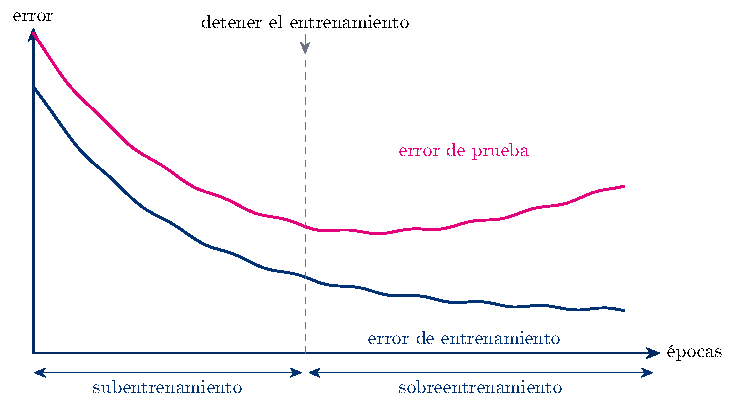
\includegraphics[max width=\linewidth]{Fig6.pdf}
\caption{Regiones de sobre y sub entrenamiento para una red neuronal.}
\label{fig6}
\end{figure}

Otro tema importante a discutir es el {\em sobre entrenamiento} y el {\em tiempo óptimo de parada} del entrenamiento. Entrenando durante un tiempo suficientemente largo (involucrando un número suficientemente grande de ciclos) el error de entrenamiento se puede hacer, en general, muy pequeño. Al principio del período de entrenamiento, el error de testeo también disminuye, hasta que se llega a un punto luego del cual comienza a crecer lentamente. Un criterio habitual de parada (parada temprana) es detener el entrenamiento cuando el error medido sobre datos no usados para entrenar, el de validación, llega a su mínimo. Si se usara el conjunto de testeo para decidir, dejaría de ser una estimación honesta de la generalización: el conjunto de testeo debe usarse una sola vez, al final. Luego de ese instante, la diferencia entre el error de testeo y el de entrenamiento comienza a crecer, un hecho que lleva al sobreajuste. Es decir, la red funciona muy bien con los datos de entrenamiento, pero no con los datos de prueba. Ver Figura~\ref{fig6}.

\section{Significado geométrico}\label{sec.c3.5}

Si $C(w, b)$ y $U(w)$ son suaves, entonces la función de costo regularizada $G(w, b) = C(w, b) + \lambda U(w)$ también resulta suave y su mínimo se realiza para
$$
(w^*, b^*) = \argmin (C(w, b) + \lambda U(w)).
$$
En este punto mínimo, el gradiente se tiene que anular. En particular $\nabla_w C(w^*, b^*) = -\lambda \nabla_w U(w^*)$. Esto significa que, con $b=b^*$ fijo, los vectores normales a las superficies de nivel de $w\mapsto C(w, b^*)$ y de $U$ son colineales (el sesgo no se regulariza, y $\partial_bC(w^*,b^*)=0$). Esto ocurre cuando las superficies de nivel son tangentes. Ver Figura \ref{fig7}.
\begin{figure}[htbp]
\centering
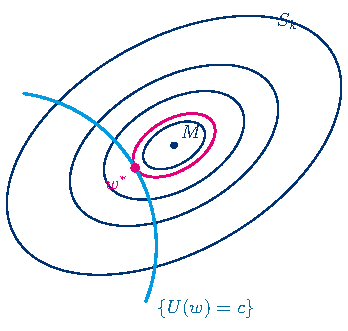
\includegraphics[max width=\linewidth]{Fig7.pdf}
\caption{La función de costo $C(w, b)$ tiene un mínimo en $M$; sus superficies de nivel vienen dadas por $S_k = \{C(w, b)=k\}$. Una de esas superficies de nivel es tangente a la superficie $\{U(w)=c\}$ en un punto en donde los gradientes $\nabla C$ y $\nabla U$ son colineales.}
\label{fig7}
\end{figure}
Como los vectores normales a las superficies de nivel son colineales y tienen sentido opuesto, resulta que $\lambda>0$.

\subsection*{La importancia de $\lambda$} Para poder entender mejor el rol del multiplicador $\lambda$, asumamos por simplicidad que $U(w)=\|w\|_2^2$. Si $w^*$ es un punto de contacto entre $\{C(w, b)=k\}$ y $\{U(w)=c\}$ (ver Figura~\ref{fig7}), entonces la ecuación $\nabla_w C(w^*, b^*) = -\lambda \nabla_w U(w^*)$ se convierte en $\nabla_w C(w^*, b^*) = -2\lambda w^*$. Esto implica que
$$
\|\nabla_w C(w^*, b^*)\| = 2\lambda\sqrt{c},
$$
 es decir que la magnitud del vector normal a la superficie $\{C(w, b)=k\}$ en $w^*$ depende tanto de $\lambda$ como de $c$. Veamos las siguientes observaciones:
 \begin{enumerate}
 \item Asumamos que $\nabla_w C(w^*, b^*) \neq 0$. Entonces valores pequeños (grandes) de $c$ se corresponden con valores grandes (pequeños) de $\lambda$. Equivalentemente, valores pequeños de $\lambda$ se corresponden a valores grandes de los pesos $w$ y valores grandes de $\lambda$ se corresponden con valores pequeños de $w$. Este razonamiento es heurístico: supone que $\|\nabla_wC(w^*,b^*)\|$ no varía demasiado al variar $\lambda$.
 
 \item Asumamos ahora que $\nabla_w C(w^*, b^*)=0$. Entonces $\lambda=0$ o $c=0$. La condición $c=0$ es equivalente a $w=0$, lo que implica que $w^*=0$, es decir que la función de costo $C(w, b)$ tiene un mínimo global en $w=0$. Dado que la mayoría de las funciones de costo no verifican esto, podemos concluir que $\lambda=0$ en este caso.
 \end{enumerate}

\subsection*{El rol de la restricción} Sea $w^* = \argmin C(w, b)$ y asumamos que $w^*\neq 0$. 

Se tienen dos casos posibles:
\begin{enumerate}
\item $w^*\in \{w\in \R^n\colon U(w)\le c\}$. Este caso corresponde al caso en que $c$ es suficientemente grande tal que el mínimo de $C(w, b)$ está contenido en el interior de la superficie $\{U(w)=c\}$. Ver Figura \ref{fig8} {\bf a}. En este caso, elegimos $\lambda=0$.

\item $w^*\not\in \{w\in \R^n\colon U(w)\le c\}$. Esta situación describe el caso en que $c$ es suficientemente pequeño para que el mínimo de $C(w, b)$ esté afuera del dominio $D_c=\{U(w)\le c\}$. En este caso, por ejemplo si $C$ es convexa, el mínimo de $C(w, b)$ sobre el dominio $D_c$ va a localizarse en el borde, sobre la superficie $\{U(w)=c\}$, en un punto $w^{**}$ por el que pase una superficie de nivel de $C(w, b)$ tangente a la superficie $\{U(w)=c\}$, ver Figura \ref{fig8} {\bf b}. Las incógnitas $w^{**}$ y $\lambda$ satisfacen las ecuaciones
$$
\partial_{w_k} C(w^{**}) = -\lambda \partial_{w_k} U(w^{**}),\quad U(w^{**})=c.
$$
Para obtener una aproximación de la solución de esta ecuación, minimizamos $G(w, b) = C(w, b) + \lambda U(w)$ usando un método de descenso de gradiente. El hiperparámetro $\lambda$ es ajustado para que el mínimo de $G$ sea lo menor posible.
\end{enumerate}
La equivalencia entre minimizar $C+\lambda U$ (penalización) y minimizar $C$ sujeto a $U\le c$ (restricción) vale, por ejemplo, cuando $C$ y $U$ son convexas, por dualidad de Lagrange; en general no es cierta.
\begin{figure}[htbp]
\centering
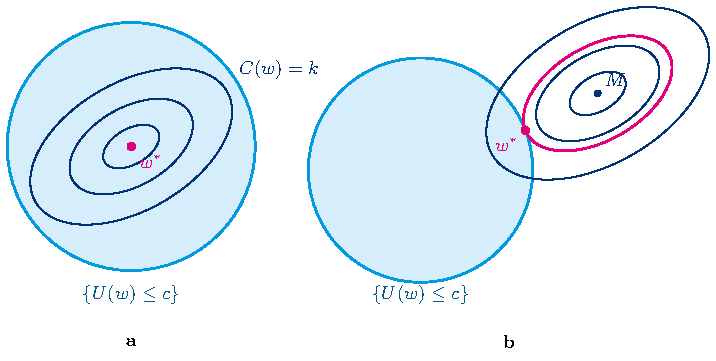
\includegraphics[max width=\linewidth]{Fig8.pdf}
\caption{La función costo $C(w, b)$ en dos posibilidades distintas: {\bf a.} $w^*\in \{U(w)\le c\}$  {\bf b.} $w^*\not\in \{U(w)\le c\}$}
\label{fig8}
\end{figure}

\subsection*{Eliminación del sobreajuste}
Hemos visto que en el caso en que el error de entrenamiento $C_\Tc(w, b)$ es pequeño, mientras que el error de testeo $C_T(w, b)$ es grande, tenemos un problema de sobreajuste.

Una forma de intentar solucionar este problema es requerir que el vector de pesos $w$ sea pequeño. La idea es que, cuanto más pequeños son los pesos, menos depende la salida de la entrada, y por lo tanto más próximos van a estar el error de testeo y el de entrenamiento. En el caso extremo $w=0$ (en todas las capas), la salida $f_{0,b}(X)$ es una constante que depende solo de los sesgos y de las funciones de activación, y es el mismo valor sea que el dato pertenezca al testeo o al entrenamiento.

Esto es solo una heurística: el modelo constante subajusta, de modo que la regularización busca un equilibrio entre ambos efectos. Una justificación cuantitativa requiere cotas de generalización (por ejemplo, en términos de la complejidad de Rademacher; ver el Capítulo~26 de S.~Shalev-Shwartz y S.~Ben-David, {\em Understanding Machine Learning}), que no veremos aquí.

\section{Resumen}\label{sec.c3.6}

Durante el proceso de aprendizaje, las redes neuronales tratan de igualar sus salidas a los objetivos dados. Este proceso de aproximación involucra el uso de funciones de costo, que miden la diferencia entre lo que es predicho (la salida) y lo que es deseado (el objetivo). Estas proximidades son de varios tipos, dependiendo de lo que la red está tratando de aprender: una función, una variable aleatoria, una densidad de probabilidad, etc. Algunas de estas funciones de costo son funciones distancia, mientras que otras no. Sin embargo todas miden la separación de la salida respecto del objetivo.

Algunas veces, para eliminar el problema de sobreajuste, la función de costo es aumentada con un término de regularización. Estos términos dependen de los pesos y tienen la tarea de minimizar el costo sujeto a pesos de magnitudes pequeñas. El coeficiente del término de regularización es un hiperparámetro que controla el compromiso entre el tamaño de los pesos y el mínimo de la función de costo. El valor de este hiperparámetro es ajustado usando el conjunto de validación.

El conjunto de datos disponibles es dividido en tres partes que son usados para los siguientes propósitos: entrenamiento, testeo y validación. Cuando la función de costo es calculada usando los datos del conjunto de entrenamiento y se optimiza, se obtiene el error de entrenamiento. Cuando se usa el conjunto de datos de testeo, se obtiene el error de testeo. Un pequeño error de entrenamiento junto a un error de testeo grande es una señal de sobreajuste. Un error de entrenamiento grande es una señal de subajuste. El propósito de la regularización es obtener un menor error de testeo.


\section{Ejercicios}\label{sec.c3.7}


\begin{ejer}
Sean $p, p_i, q, q_i$ funciones positivas en $\R$ (de modo que $S(p,q)=-\int_\R p\ln q\,dx$ tenga sentido cuando la integral converge) y $\alpha\in \R$. Mostrar que se verifican las siguientes propiedades:
\begin{itemize}
\item[(a)] $S(p_1 + p_2, q) = S(p_1, q) + S(p_2, q)$

\item[(b)] $S(\alpha p, q) = \alpha S(p, q) = S(p, q^\alpha)$

\item [(c)] $S(p, q_1 q_2) = S(p, q_1) + S(p, q_2)$.
\end{itemize}
\end{ejer}

\begin{ejer}
Verificar que la entropía cruzada verifica
$$
S(p, q)\ge 1-\int_\R p(x) q(x)\, dx.
$$
\end{ejer}

\begin{ejer}
Sea $X$ una variable aleatoria discreta. Mostrar que $H(X)\ge 0$.
\end{ejer}

\begin{ejer}
Asumamos que la variable objetivo $Z$ es $\Ec-$medible. ¿Cuál es la función de error cuadrático medio en este caso?
\end{ejer}

\begin{ejer}
Supongamos que la red tiene una función de entrada-salida $f_{w, b}$ lineal en $w$ y en $b$. Probar que la función de costo
$$
C(w, b) = \sum_{i=1}^n (f_{w, b}(x_i) - z_i)^2,
$$
alcanza su mínimo en algún par de parámetros $(w^*, b^*)$ (que es único si la matriz de datos extendida tiene rango completo), y que este par puede calcularse explícitamente a partir de las ecuaciones normales.
\end{ejer}

%%%%%%%%%%%%%%%%%%%%%%%%%%%%%%%%%%%%%%%%
%% CAPITULO 4 %%%%%%%%%%%%%%%%%%%%%%%%%%%%%%%
%%%%%%%%%%%%%%%%%%%%%%%%%%%%%%%%%%%%%%%%

\chapter{Algoritmos de minimización}\label{cap4}

El proceso de aprendizaje en aprendizaje supervisado consiste en ajustar los parámetros de la red (pesos y sesgos) hasta que una cierta función de costo es minimizada. Dado que el número de parámetros es muy grande, es necesario contar con un algoritmo de minimización que sea robusto. En este capítulo veremos algunos algoritmos de minimización y discutiremos ventajas y desventajas de cada uno de estos algoritmos.

El capítulo estudia cómo minimizar una función de costo. Primero, las propiedades generales de los mínimos (Sección~\ref{sec.c4.1}); después, los algoritmos de descenso de gradiente (Sección~\ref{sec.c4.2}), que son el método de entrenamiento básico, y por último la búsqueda estocástica (Sección~\ref{sec.c4.3}). Corresponde al Capítulo~4 de~\cite{Calin}.

\section{Propiedades generales de los mínimos}\label{sec.c4.1}

En esta sección revisaremos algunos conceptos básicos sobre los mínimos de funciones de una o varias variables. Estas técnicas analíticas teóricas sólo son eficientes si el número de variables no es muy grande. Sin embargo, en aprendizaje automático, el número de variables es del orden de miles, o más. Luego, estos métodos analíticos clásicos no son eficientes para aplicaciones concretas. Los discutiremos por completitud y porque son la base de construcción de métodos más sofisticados y robustos.

\subsection{Funciones de una variable real}

Recordemos que si tenemos una función continua $f\colon [a, b]\to \R$, definida en un intervalo compacto, esta es acotada y alcanza sus cotas dentro del intervalo $[a, b]$. Es decir, existe (por lo menos) un valor $c\in [a, b]$ tal que 
$$
f(c) = \min_{x\in [a, b]} f(x).
$$
Este es el {\em mínimo global} para $f(x)$. Sin embargo, la función puede también tener mínimos locales. Más aún, si el valor mínimo (ya sea local o global) se encuentra en el interior del intervalo, i.e. $c\in (a, b)$, y si la función es diferenciable, entonces tenemos que $f'(c)=0$. Geométricamente, esto significa que la recta tangente al gráfico de $y=f(x)$ en el punto $(c, f(c))$ es horizontal, Recordemos que esta condición es necesaria, pero no suficiente. Si, adicionalmente, la función es convexa (es decir, verifica $f''(x)\ge 0$), entonces esta condición resulta suficiente.

\subsection{Funciones de varias variables reales}

Sea $K$ un conjunto compacto en $\R^n$, es decir es un conjunto cerrado y acotado. Por ejemplo, $K=[a_1, b_1]\times\cdots\times [a_n, b_n]$ con $a_i, b_i\in\R$, o $K=\{\xx\in\R^n\colon \|\xx\|_2\le R\}$, con $R>0$. Si $f\colon K\to\R$ es continua, entonces existe un punto $\cc\in K$ tal que $f$ alcanza su mínimo y si, adicionalmente, $f$ es diferenciable en $\cc$ y el punto $\cc$ está en el interior del compacto $K$, se tiene que
$$
\frac{\partial f}{\partial x_i}(\cc) = 0,\quad i=1,\dots,n.
$$
En notación vectorial, este sistema de ecuaciones se puede escribir como $\nabla f(\cc) = 0$.

Esta condición geométricamente es equivalente a que el plano tangente al gráfico $z=f(\xx)$ en el punto $(\cc, f(\cc))$ sea horizontal (i.e. paralelo al hiperplano $z=0$ en $\R^{n+1} = \{(\xx, z)\colon \xx\in\R^n, z\in\R\}$).

Si $f$ es de clase $C^2$, el desarrollo de Taylor de orden 2 de $f(\xx)$ en un entorno de $\xx=\cc$ es
\begin{align*}
f(\xx) = & f(\cc) + \sum_{i=1}^n \frac{\partial f}{\partial x_i}(\cc) (x_i-c_i)\\
& + \frac12 \sum_{j, k = 1}^n \frac{\partial^2 f}{\partial x_j\partial x_k}(\cc)(x_j-c_j)(x_k-c_k) + o(\|\xx-\cc\|^2)
\end{align*}
Si llamamos $Hf$ o $D^2f$ a la matriz Hessiana o matriz de derivadas segundas, dada por
$$
Hf(\xx) = D^2f(\xx) = \begin{pmatrix} \frac{\partial^2 f}{\partial x_1^2}(\xx) & \frac{\partial^2 f}{\partial x_1\partial x_2}(\xx)& \cdots & \frac{\partial^2 f}{\partial x_1\partial x_n}(\xx)\\
\frac{\partial^2 f}{\partial x_2\partial x_1}(\xx) & \frac{\partial^2 f}{\partial x_2^2}(\xx)& \cdots & \frac{\partial^2 f}{\partial x_2\partial x_n}(\xx)\\
\vdots & \vdots & \ddots & \vdots\\
\frac{\partial^2 f}{\partial x_n\partial x_1}(\xx) & \frac{\partial^2 f}{\partial x_n\partial x_2}(\xx) & \cdots & \frac{\partial^2 f}{\partial x_n^2}(\xx)
\end{pmatrix},
$$
el desarrollo de Taylor se puede reescribir como
$$
f(\xx) = f(\cc) + \nabla f(\cc)\cdot(\xx - \cc) + \frac12 (\xx-\cc) Hf(\cc) (\xx-\cc)^t + o(\|\xx-\cc\|^2).
$$
Observemos que la matriz Hessiana resulta simétrica si $f\in C^2$, es decir $Hf(\xx) = Hf(\xx)^t$.

Si se verifica que $\nabla f(\cc)=0$, entonces el desarrollo de Taylor queda
$$
f(\xx) = f(\cc)  + \frac12 (\xx-\cc) Hf(\cc) (\xx-\cc)^t + o(\|\xx-\cc\|^2).
$$

Asumamos ahora que la matriz Hessiana es definida positiva, i.e.
$$
\vv Hf(\cc)\vv^t>0,\quad \forall \vv\in \R^n\setminus \{0\}.
$$
Si llamamos $\Phi(\xx) = \xx Hf(\cc)\xx^t$ la forma cuadrática asociada a la matriz Hessiana, esta es una función continua y si llamamos $\Sb=\{\xx\in\R^n\colon \|\xx\|=1\}$ a la esfera unidad, este conjunto resulta compacto y por ende existe $\yy\in \Sb$ tal que
$$
0<m=\Phi(\yy) = \min_{\xx\in \Sb}\Phi(\xx).
$$
Por otro lado, observemos que la forma cuadrática es {\em homogénea de grado 2}, es decir:
$$
\Phi(\lambda\xx) = (\lambda\xx)Hf(\cc)(\lambda\xx)^t = \lambda^2 (\xx Hf(\cc)\xx^t) = \lambda^2\Phi(\xx).
$$
Luego, si $\xx\neq 0$, tenemos que $\xx/\|\xx\|\in \Sb$, de donde obtenemos que
$$
0<m\le \Phi\left(\frac{\xx}{\|\xx\|}\right) = \frac{1}{\|\xx\|^2} \Phi(\xx).
$$
Se tiene entonces la siguiente desigualdad para la matriz Hessiana:
\begin{equation}\label{H>0}
\xx Hf(\cc)\xx^t\ge m \|\xx\|^2,\qquad (m>0).
\end{equation}
Con la ayuda de \eqref{H>0} podemos demostrar el siguiente criterio
\begin{prop}
Sea $f$ una función de clase $C^2$ y $\cc\in \R^n$ una solución de $\nabla f(\cc)=0$. Si la matriz Hessiana de $f$ en $\cc$. $Hf(\cc)$ es definida positiva, entonces $\cc$ es un mínimo local de $f$.
\end{prop}

\begin{proof}
Por lo visto anteriormente, tenemos que $f$ admite el desarrollo
\begin{equation}\label{est1}
f(\xx) - f(\cc) = \frac12 (\xx-\cc)Hf(\cc)(\xx-\cc)^t + o(\|\xx-\cc\|^2)\ge \frac{m}{2} \|\xx-\cc\|^2 + o(\|\xx-\cc\|^2),
\end{equation}
donde hemos usado \eqref{H>0} en la desigualdad. El término de error, verifica
$$
\lim_{\xx\to\cc} \frac{o(\|\xx-\cc\|^2)}{\|\xx-\cc\|^2} = 0,
$$
luego, dado $\ve>0$ existe $\delta>0$ tal que
$$
\frac{|o(\|\xx-\cc\|^2)|}{\|\xx-\cc\|^2}<\ve,\quad \text{si } \|\xx-\cc\|<\delta.
$$
En particular, tomando $\ve=m/4$, tenemos que existe $\delta>0$ tal que
\begin{equation}\label{est2}
-\frac{m}{4} \|\xx-\cc\|^2 \le o(\|\xx-\cc\|^2) \quad \text{si } \|\xx-\cc\|<\delta.
\end{equation}
Combinando \eqref{est1} y \eqref{est2} obtenemos
$$
f(\xx)-f(\cc) \ge \frac{m}{4} \|\xx-\cc\|^2\ge 0,
$$
de donde obtenemos el resultado.
\end{proof}


\begin{ejem}[Matriz Hessiana en dimensión 2]
Si $f$ es de clase $C^2$ en $\R^2$, entonces su matriz Hessiana tiene la forma
$$
Hf = \begin{pmatrix} f_{xx} & f_{xy}\\f_{xy} & f_{yy}\end{pmatrix}.
$$
Si $\vv = (a, b)\in \R^2$, entonces la forma cuadrática asociada es de la forma
$$
\vv Hf \vv^t = f_{xx} a^2 + 2f_{xy} ab + f_{yy} b^2.
$$
Realizando cálculos elementales, si $f_{xx}\neq0$ esta expresión puede escribirse como
$$
\vv Hf \vv^t = f_{xx} \left( a+ \frac{f_{xy}}{f_{xx}} b\right)^2 + \frac{b^2}{f_{xx}}\underbrace{(f_{xx}f_{yy}-f_{xy}^2)}_{\det Hf}.
$$
De esta expresión se deduce fácilmente lo siguiente:
\begin{enumerate}
\item Si $f_{xx}>0$ y $\det Hf >0$, entonces $Hf$ es definida positiva.
\item Si $f_{xx}<0$ y $\det Hf>0$, entonces $Hf$ es definida negativa.
\item Si $\det Hf<0$, entonces $Hf$ es indefinida (esto vale también si $f_{xx}=0$, pues $\det Hf$ es el producto de los autovalores, que entonces tienen signos opuestos).
\item Si $\det Hf=0$, entonces $Hf$ es semidefinida (algún autovalor es nulo) y estos criterios no deciden. Para el caso general conviene el criterio de Sylvester.
\end{enumerate}
\end{ejem}

\begin{ejem}[Funciones cuadráticas]
Sea $A\in \R^{n\times n}$ una matriz simétrica y definida positiva y sean $\bb \in \R^n$ y $d\in \R$. Consideremos la siguiente función
$$
f(\xx) = \frac12 \xx A\xx^t - \bb\cdot\xx + d,\quad \xx\in\R^n.
$$
En coordenadas, 
$$
f(x_1,\dots,x_n) = \frac12\sum_{i, j=1}^n a_{ij} x_i x_j - \sum_{k=1}^n b_k x_k + d.
$$
La función $f\colon \R^n\to\R$ resulta suave con $(\nabla f(\xx))^t = A\xx^t - \bb^t$, $Hf(\xx) = A$. Al ser $A$ definida positiva, $f$ resulta convexa, tiene un único punto crítico dado por $\cc^t= A^{-1}\bb^t$ que resulta ser un mínimo global.

Si a la función cuadrática $f$ la restringimos a un conjunto compacto $K\subset \R^n$, puede ser que el punto crítico $\cc$ pertenezca o no a $K$. Luego, en el caso en que $\cc\not\in K$ no podemos hallar los mínimos como puntos críticos de $f$. Más aún, los mínimos de $f$ en $K$ van a pertenecer a la frontera de $K$, $\partial K$ y para hallarlos habrá que utilizar algún método alternativo (p.ej. multiplicadores de Lagrange).
\end{ejem}

\section{Algoritmos de descenso de gradiente}\label{sec.c4.2}

El algoritmo de descenso de gradiente es un procedimiento para hallar el mínimo de una función navegando a través de las curvas de nivel asociadas siguiendo la dirección de máximo decrecimiento. 

\subsection{Conjuntos de nivel}\label{sec.perp}

Consideremos a la función $z=f(\xx)$, $\xx\in D\subset \R^n$ con $n\ge 2$ y definamos el conjunto de nivel $c\in \R$ como
$$
\Sw_c = f^{-1}(\{c\}) = \{\xx\in D\colon f(\xx)=c\}.
$$
El {\em Teorema de la función implícita} nos permite asegurar que si $f\in C^1$ y $\nabla f(\xx)\neq 0$ para $\xx\in \Sw_c$, el conjunto de nivel $\Sw_c$ resulta ser una hipersuperficie (es decir, una superficie de dimensión $n-1$). A la familia $\{\Sw_c\}_{c\in\R}$ se la llama la familia de {\em hipersuperficies de nivel} de la función $f$. Para $n=2$ se las llama las {\em curvas de nivel}. Geométricamente, las hipersuperficies de nivel se obtienen intersectando el gráfico $z=f(\xx)$ con el plano horizontal $z=c$. Ver Figura~\ref{fig9}.
\begin{figure}[htbp]
\centering
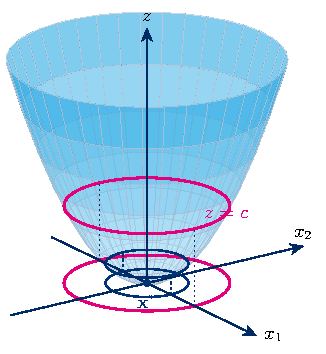
\includegraphics[max width=\linewidth]{Fig9.pdf}
\caption{Conjuntos de nivel para la función $z=f(\xx)$.}
\label{fig9}
\end{figure}

\begin{prop}\label{perp}
El gradiente $\nabla f$ es perpendicular a $\Sw_c$.
\end{prop}

\begin{proof}
Sea $\xx_0\in \Sw_c$ y consideremos una curva $\xx(t)$, $t\in (-\delta, \delta)$ tal que $\xx(0)=\xx_0$ y $\xx(t)\in \Sw_c$ para todo $t\in (-\delta, \delta)$. Luego, el vector tangente a la curva en $t=0$, $\vv = \xx'(0)$ es un vector tangente a $\Sw_c$ en el punto $\xx_0$.

Por otro lado, como $\xx(t)\in \Sw_c$ para todo $t\in (-\delta, \delta)$, se tiene que $f(\xx(t)) = c$ para todo $t\in (-\delta, \delta)$. Luego si llamamos $\phi(t)=f(\xx(t))$, tenemos que $\phi\colon (-\delta,\delta)\to \R$ es constante, por ende $\phi'(t)=0$. Pero
$$
0=\phi'(t) = \frac{d}{dt}f(\xx(t)) = \nabla f(\xx(t)) \cdot \xx'(t).
$$
Evaluando en $t=0$ obtenemos
$$
\nabla f(\xx_0) \cdot \vv = 0.
$$
Como $\vv$ es un vector tangente arbitrario, concluimos lo deseado.
\end{proof}

Asumamos ahora que la función $z=f(\xx)$ tiene un mínimo local estricto en $\xx^*\in D$, es decir, existe un entorno $\Vc$ de $\xx^*$ tal que $f(\xx^*)<f(\xx)$ para todo $\xx\in \Vc\setminus\{\xx^*\}$. Notemos por $z^*=f(\xx^*)$ el valor mínimo de $f$ en $\Vc$. Adicionalmente, asumamos que $\nabla f(\xx)\neq 0$ para $\xx\in \Vc\setminus\{\xx^*\}$. Sea $B\subset\Vc$ una bola cerrada centrada en $\xx^*$. Como $f>z^*$ sobre la esfera $\partial B$ (que es compacta), existe $m_B=\min_{\partial B}f>z^*$. Para $c\in(z^*,m_B)$, el conjunto $\{\xx\in B\colon f(\xx)\le c\}$ es compacto, está contenido en el interior de $B$, y crece con $c$. Dentro de $B$ tenemos $\Sw_{z^*}\cap B=\{\xx^*\}$ y los conjuntos $\Sw_c\cap B$, $c\in(z^*,m_B)$, son hipersuperficies (porque $\nabla f\ne0$) anidadas: cada una encierra a las anteriores. Ver Figura~\ref{fig9}.

La demostración de \cite[Lemma 4.2.2]{Calin} plantea un sistema sobredeterminado (se impone a la vez $\alpha'(0)=v$ y $\alpha'(0)=\nabla f(\xx^*)=0$), y los Teoremas 4.2.3 y 4.2.4 de ese libro se apoyan en ella. En su reemplazo damos una demostración alternativa de un resultado análogo al enunciado en \cite[Theorem 4.2.3]{Calin}.

\begin{teo}\label{4.2.2}
Asumamos que $f\colon D\subset\R^n\to\R$ es de clase $C^2$, que $\xx^*\in D$ es un mínimo local estricto de $f$ y que existe un entorno $\Vc\subset D$ de $\xx^*$ tal que $\nabla f(\xx)\neq 0$ para $\xx\in \Vc\setminus\{\xx^*\}$. Entonces existe un entorno abierto $W\subset\Vc$ de $\xx^*$ tal que, dado $\xx_0\in W\setminus\{\xx^*\}$, existe una curva continua $\gamma\colon [0,1]\to \R^n$, de clase $C^1$ en $[0,1)$, tal que
\begin{enumerate}
\item $\gamma(0) = \xx_0$;
\item $\gamma(1) = \xx^*$;
\item $\gamma'(t)$ es perpendicular a $\Sw_{f(\gamma(t))}$ para $t\in [0, 1)$.
\end{enumerate}
\end{teo}

\begin{proof}
{\em Paso 1: el entorno $W$.} Sean $B$, $m_B$ como arriba, fijemos $c\in(z^*,m_B)$ y definamos
$$
K_c=\{\xx\in B\colon f(\xx)\le c\},\qquad W=\{\xx\in \operatorname{int}B\colon f(\xx)<c\}.
$$
$K_c$ es compacto y $W$ es un entorno abierto de $\xx^*$.

{\em Paso 2: el flujo del gradiente.} Dado $\xx_0\in W\setminus\{\xx^*\}$, sea $\alpha$ la solución maximal de
\begin{equation}\label{grad}
\alpha' = -\nabla f(\alpha),\qquad \alpha(0)=\xx_0
\end{equation}
(como $f\in C^2$, el campo $\nabla f$ es $C^1$, y hay existencia y unicidad). Se tiene $\frac{d}{dt}f(\alpha(t))=-\|\nabla f(\alpha(t))\|^2\le0$, de modo que $f(\alpha(t))\le f(\xx_0)<c$. Entonces $\alpha$ no puede salir de $B$, pues para hacerlo tendría que cruzar $\partial B$, donde $f\ge m_B>c$. Luego $\alpha(t)\in K_c$ (compacto) para todo $t$ y, por lo tanto, la solución existe para todo $t\ge0$. Además $\alpha(t)\neq\xx^*$ para todo $t$: como $\xx^*$ es un equilibrio de \eqref{grad}, si $\alpha(t_0)=\xx^*$ para algún $t_0$, la unicidad daría $\alpha\equiv\xx^*$, contra $\alpha(0)=\xx_0\ne\xx^*$. En consecuencia, $\nabla f(\alpha(t))\ne0$ para todo $t\ge0$.

{\em Paso 3: convergencia.} La función $t\mapsto f(\alpha(t))$ es decreciente y está acotada inferiormente por $z^*$; sea $\ell\ge z^*$ su límite. Si fuera $\ell>z^*$, entonces $\alpha(t)$ permanecería en el compacto $\{\xx\in K_c\colon f(\xx)\ge\ell\}$, que no contiene a $\xx^*$ y está contenido en $\Vc\setminus\{\xx^*\}$, donde $\|\nabla f\|$ es continua y no se anula; luego $\|\nabla f\|\ge\mu>0$ en él y resultaría $f(\alpha(t))\le f(\xx_0)-\mu^2t\to-\infty$, un absurdo. Por lo tanto, $f(\alpha(t))\to z^*$. Si $t_k\to\infty$, por compacidad una subsucesión de $\alpha(t_k)$ converge a algún $\yy\in K_c$ con $f(\yy)=z^*$; como $\xx^*$ es el único punto de $B$ con $f=z^*$, resulta $\yy=\xx^*$. Esto prueba que $\alpha(t)\to\xx^*$ cuando $t\to\infty$.

{\em Paso 4: reparametrización.} La curva $\alpha\colon[0,\infty)\to\R^n$ verifica $\alpha(0)=\xx_0$, $\alpha(t)\to\xx^*$ y $\alpha'(t)=-\nabla f(\alpha(t))$, que es perpendicular a $\Sw_{f(\alpha(t))}$ por la Proposición~\ref{perp}. Para tener una curva definida en $[0,1]$ la reparametrizamos:
$$
\gamma(t) = \begin{cases}
\xx^* & \text{si } t=1\\
\alpha\!\left(\tfrac{t}{1-t}\right) & \text{si } 0\le t< 1.
\end{cases}
$$
Como $t/(1-t)\to\infty$ cuando $t\to1^-$, $\gamma$ es continua, $\gamma(0) = \xx_0$ y, para $t\in[0,1)$,
$$
\gamma'(t) = \frac{1}{(1-t)^2}\alpha'\!\left(\tfrac{t}{1-t}\right) = -\frac{1}{(1-t)^2}\nabla f\!\left(\gamma(t)\right),
$$
que es perpendicular a $\Sw_{f(\gamma(t))}$ por la Proposición~\ref{perp}.
\end{proof}

La construcción de la curva del Teorema \ref{4.2.2} no es de utilidad a efectos computacionales. Para poder implementar la construcción de la curva, necesitamos poder aproximarla por una poligonal $\B_m = [\xx_0 \xx_1 \cdots \xx_m]$ con las siguientes propiedades:
\begin{enumerate}
\item $\xx_k\in \Sw_{c_k}$;\label{prop1}
\item $c_{k+1}<c_k$, para $k=0,1,\dots,m-1$;\label{prop2}
\item el segmento $[\xx_k \xx_{k+1}]$ es perpendicular a $\Sw_{c_k}$.\label{prop3}
\end{enumerate}

El algoritmo de construcción es el siguiente: empezamos con un punto $\xx_0$ en un entorno del mínimo $\xx^*$. Elegimos un parámetro $\tau>0$ pequeño y nos movemos una distancia $\tau$ de $\xx_0$ siguiendo la dirección normal a $S_{c_0}$ hacia el interior de la región, es decir  en la dirección de $-\nabla f(\xx_0)$:
$$
\xx_1 = \xx_0 - \tau \frac{\nabla f(\xx_0)}{\|\nabla f(\xx_0)\|}.
$$
Repetimos este procedimiento y así obtenemos la sucesión de puntos
$$
\xx_{k+1} = \xx_k - \tau \frac{\nabla f(\xx_k)}{\|\nabla f(\xx_k)\|}. 
$$
Este procedimiento se continúa y luego de $m$ pasos se llega al punto $\xx_m$ que esperamos sea una buena aproximación del punto buscado $\xx^*$.

¿Cómo se puede elegir el número de pasos $m$? En otras palabras, ¿cómo sabemos cuándo detener el algoritmo? El mejor criterio para detener el algoritmo es continuar siempre que se verifique que $c_{k+1}<c_k$. Para un tamaño de paso $\tau>0$ fijo, el algoritmo se detiene en el primer $m$ tal que $c_{m+1}\ge c_m$; esto ocurre, en la práctica, cuando el paso, que tiene longitud fija $\tau$, ya no permite acercarse más a $\xx^*$. Heurísticamente, mientras más pequeño sea el paso $\tau$, más grande será el orden de parada $m$ y más próximos estaremos de $\xx^*$; y cuando $\tau\to 0$, la línea poligonal $\B_m$ aproxima a la curva $\gamma$ dada por el Teorema \ref{4.2.2}.


Si el algoritmo se detiene luego de $m$ pasos, se tienen las siguientes cotas
\begin{equation}\label{cotas}
\|\xx_0-\xx^*\| - m\tau\le \|\xx_m - \xx^*\|\le \diam(\Sw_{c_m}),
\end{equation}
donde $\diam(\Sw_c)$ es el diámetro del conjunto $\Sw_c$ (la segunda desigualdad vale cuando $\xx^*$ pertenece a la envoltura convexa de $\Sw_{c_m}$, por ejemplo si $\Sw_{c_m}$ es el borde de una región convexa que contiene a $\xx^*$). De la primera desigualdad se deduce una cota inferior para el número de pasos:
$$
m\ge\frac{\|\xx_0-\xx^*\|-\|\xx_m-\xx^*\|}{\tau}.
$$

Para demostrar las cotas de \eqref{cotas}, se razona como sigue: Usando la desigualdad triangular
\begin{align*}
\|\xx_0-\xx^*\|&\le \|\xx_0-\xx_1\| + \|\xx_1-\xx_2\| +\cdots +\|\xx_{m-1}-\xx_m\| + \|\xx_m-\xx^*\|\\
&= m\tau +  \|\xx_m-\xx^*\|.
\end{align*}
Para la segunda desigualdad de \eqref{cotas}, usando que $\xx^*\in\operatorname{conv}(\Sw_{c_m})$ y que $\yy\mapsto\|\xx_m-\yy\|$ es convexa, se tiene
$$
\|\xx^*-\xx_m\|\le \max_{\yy\in \Sw_{c_m}}\|\xx^*-\yy\| \le \sup_{\xx, \yy\in \Sw_{c_m}} \|\xx-\yy\| = \diam(\Sw_{c_m}).
$$
\begin{figure}[htbp]
\centering
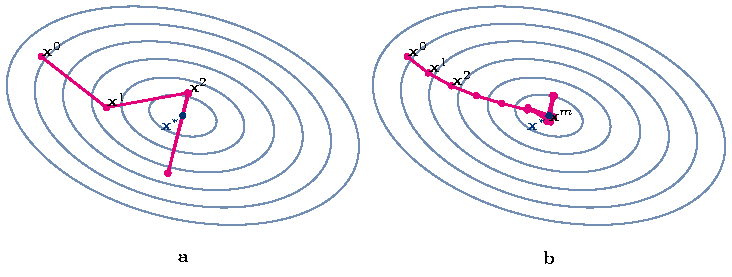
\includegraphics[max width=\linewidth]{Fig10.pdf}
\caption{La poligonal $\B_m=[\xx_0\cdots \xx_m]$ en dos casos: {\bf a}. El paso $\tau$ es grande. {\bf b}. El paso $\tau$ es pequeño.}
\label{fig10}
\end{figure}
La elección del paso $\tau$ en la construcción de la poligonal es muy importante. Se pueden tener los casos:
\begin{enumerate}
\item Si $\tau$ es grande, el algoritmo para muy tempranamente y no se obtiene una buena aproximación de $\xx^*$. Ver Figura~\ref{fig10} {\bf a};

\item Si $\tau$ es demasiado pequeño, la cantidad de pasos que se tienen es muy grande y puede ser muy costoso computacionalmente. Ver Figura~\ref{fig10} {\bf b}.
\end{enumerate}
En general, el tamaño del paso $\tau$ resulta de un compromiso entre el margen de error y el tiempo de corrida de la aplicación. Más adelante formalizaremos esta idea.


\subsection{Derivadas direccionales}

Otro concepto que usaremos es el de {\em derivada direccional}, que mide la tasa de variación instantánea de una función en un punto al moverse en una dirección dada. Más precisamente, si $\uu$ es un vector unitario en $\R^n$, $f\colon U\subset \R^n\to \R$ y $\xx_0\in U$, la derivada direccional de $f$ en $\xx_0$ en la dirección $\uu$ se define como
$$
\frac{\partial f}{\partial \uu}(\xx_0) = \lim_{t\to 0} \frac{f(\xx_0+t\uu) - f(\xx_0)}{t},
$$
cuando ese límite existe.

Si la función $f$ es diferenciable en $\xx_0$ entonces la derivada direccional en $\xx_0$ existe en cualquier dirección $\uu$ y la misma se calcula como
$$
\frac{\partial f}{\partial \uu}(\xx_0) = \nabla f(\xx_0)\cdot\uu.
$$

\subsection{El método de descenso más rápido}

El {\em método de descenso más rápido} ({\em steepest descent method} en inglés), también llamado {\em método de descenso de gradiente}, es un método numérico basado en un algoritmo voraz (greedy algorithm) por el cual el mínimo de una función es buscado dirigiendo cada paso en la dirección en donde la función decrece más rápidamente.

Para aplicar este método, estamos interesados en encontrar una dirección unitaria $\uu$ en la cual $f$ decrezca tanto como sea posible en un paso de tamaño $\tau$. Para eso, usamos la aproximación lineal
$$
f(\xx_0+\tau\uu) - f(\xx_0) = \tau \nabla f(\xx_0)\cdot \uu + o(\tau).
$$
Como asumimos que $0<\tau\ll 1$, podemos despreciar el efecto del término de error $o(\tau)$ (que es $O(\tau^2)$ si $f\in C^2$). Luego, para obtener la dirección $\uu$ que haga la variación lo más negativo posible, usamos la desigualdad de Cauchy--Schwarz para el producto escalar
$$
-\|\nabla f(\xx_0)\| \|\uu\|\le \nabla f(\xx_0)\cdot \uu\le \|\nabla f(\xx_0)\| \|\uu\|.
$$
Como $\|\uu\|=1$ es fácil ver que la igualdad inferior es alcanzada si y sólo si
$$
\uu = -\frac{\nabla f(\xx_0)}{\|\nabla f(\xx_0)\|}.
$$
Luego, el cambio más grande en la función es aproximadamente igual a
$$
f(\xx_0+\tau\uu) - f(\xx_0) \simeq \tau \nabla f(\xx_0)\cdot \uu = -\tau\|\nabla f(\xx_0)\|.
$$
La constante $\tau$ es llamada el {\em paso}. De la relación previa, el cambio en la función en cada paso es proporcional a la magnitud del gradiente y al paso.

El algoritmo consiste en la siguiente iteración que construye la siguiente sucesión $\{\xx_k\}_{k\ge 0}$:
\begin{enumerate}
\item Elegir un punto inicial $\xx_0$ (idealmente, en la cuenca de atracción de un mínimo de $f$).

\item Construir la sucesión $\{\xx_k\}_{k\ge 0}$ usando la iteración
\begin{equation}\label{iteracion}
\xx_{k+1} = \xx_k - \tau \frac{\nabla f(\xx_k)}{\|\nabla f(\xx_k)\|}.
\end{equation}
\end{enumerate}
Esta construcción garantiza un cambio negativo en la función objetivo que es dado por $f(\xx_{k+1}) - f(\xx_k)\simeq -\tau\|\nabla f(\xx_k)\|<0$.

Notemos que el segmento $[\xx_k \xx_{k+1}]$ es perpendicular a la hipersuperficie $\Sw_{f(\xx_k)}$. Luego, obtenemos la poligonal $\B_m=[\xx_0 \xx_1\cdots \xx_m]$ de la Sección \ref{sec.perp}, que es una aproximación de la curva $\gamma$ dada en el Teorema \ref{4.2.2}.

Sin embargo esta construcción tiene un inconveniente, que arreglaremos en breve. Como $\|\xx_{k+1}-\xx_k\|=\tau>0$, la sucesión aproximante $\{\xx_k\}_{k\ge 0}$ no converge, luego puede fácilmente perder el punto mínimo $\xx^*$. Para superar este problema, vamos a utilizar un paso $\tau_k$ variable en el sentido que se vuelva más pequeño cuando la función cambie más lentamente (cuando el gradiente sea pequeño). Asumiremos que el paso es proporcional al tamaño del gradiente de $f$ con una constante de proporcionalidad $\eta>0$, es decir $\tau_k = \eta \|\nabla f(\xx_k)\|$. (De aquí en adelante, la {\em tasa de aprendizaje} es $\eta$; el símbolo $\tau$ queda para el paso normalizado de \eqref{iteracion}.) Entonces la iteración \eqref{iteracion} resulta
\begin{equation}\label{iteracion2}
\xx_{k+1} = \xx_k - \eta \nabla f(\xx_k).
\end{equation}

\begin{prop}\label{converge} Con las hipótesis del Teorema \ref{4.2.2}, supongamos además que la sucesión $\{\xx_k\}_{k\ge 0}$ definida en \eqref{iteracion2} está contenida en un compacto $K\subset\Vc$. Entonces $\{\xx_k\}$ resulta convergente si y sólo si la sucesión de gradientes tiende a 0, $\nabla f(\xx_k)\to 0$ cuando $k\to\infty$.
\end{prop}

La demostración de \cite{Calin} de la implicación ``$\Leftarrow$'' no es correcta (estima $\|\xx^{n+p}-\xx^n\|$ con $p$ fijo, lo que no alcanza para probar que la sucesión es de Cauchy). Para subsanarlo, necesitamos un lema de espacios métricos.

\begin{lema}\label{acumulacion}
Sea $(X, d)$ un espacio métrico y sea $\{x_n\}_{n\in\N}\subset X$ una sucesión con la siguiente propiedad: Existe $x_0\in X$ tal que para toda subsucesión $\{x_{n_k}\}_{k\in\N}\subset \{x_n\}_{n\in\N}$ existe una sub-subsucesión $\{x_{n_{k_j}}\}_{j\in\N}\subset \{x_{n_k}\}_{k\in\N}$ tal que $x_{n_{k_j}}\to x_0$ cuando $j\to\infty$. Entonces $x_n\to x_0$ cuando $n\to\infty$.
\end{lema}

\begin{proof}
Supongamos que $x_n\not\to x_0$ cuando $n\to\infty$. Entonces existe $\ve>0$ tal que $d(x_n, x_0)\ge \ve$ para infinitos $n\in\N$. Luego, existe una subsucesión $\{x_{n_k}\}_{k\in\N}\subset\{x_n\}_{n\in\N}$ tal que $d(x_{n_k}, x_0)\ge \ve$ para todo $k\in\N$. Pero entonces existe una sub-subsucesión $\{x_{n_{k_j}}\}_{j\in\N}\subset \{x_{n_k}\}_{k\in\N}$ tal que $x_{n_{k_j}}\to x_0$ con lo cual $d(x_{n_{k_j}}, x_0)<\ve$ si $j\ge N$, lo que es un absurdo y el lema queda demostrado.
\end{proof}

Ahora sí, podemos demostrar la Proposición \ref{converge}
\begin{proof}[Demostración de la Proposición \ref{converge}]
Asumamos primero que $\{\xx_k\}_{k\ge 0}$ es convergente. De \eqref{iteracion2} tenemos que
$$
\|\xx_{k+1}-\xx_k\| = \eta \|\nabla f(\xx_k)\|.
$$
Como la sucesión es convergente, el lado izquierdo tiende a 0, lo que prueba lo deseado. 

Asumamos ahora que $\nabla f(\xx_k)\to 0$. Para ver que $\{\xx_k\}_{k\ge 0}$ es convergente usaremos el Lema \ref{acumulacion}. Para eso, tomemos $\{\xx_{k_j}\}_{j\in\N}\subset \{\xx_k\}_{k\in\N}$. Como la sucesión original $\{\xx_k\}_{k\in\N}$ está contenida en el compacto $K$, también lo es la subsucesión  $\{\xx_{k_j}\}_{j\in\N}$. Luego existe una sub-subsucesión $\{\xx_{k_{j_i}}\}_{i\in\N}\subset \{\xx_{k_j}\}_{j\in\N}$ convergente. Sea $\xx_0 = \lim_{i\to\infty} \xx_{k_{j_i}}$. Por hipótesis, tenemos que 
$$
\nabla f(\xx_0) = \lim_{i\to\infty}\nabla f(\xx_{k_{j_i}}) = 0.
$$
Como $K$ es cerrado, $\xx_0\in K$, y como en $\Vc$ el único punto crítico de $f$ es $\xx^*$, sigue que $\xx_0=\xx^*$ y por el Lema \ref{acumulacion} concluimos que $\xx_k\to\xx^*$.

Esto concluye la demostración.
\end{proof}

Observemos que si $f$ es de clase $C^1$ y estamos en las hipótesis de la Proposición \ref{converge}, entonces $\xx_k\to \xx^*$ y $\nabla f(\xx_k)\to \nabla f(\xx^*) = 0$.


\begin{ejem}
Consideremos la función $f\colon (0,1)\times (-2,2)\to\R$ dada por $f(x, y)=\tfrac12 y^2 - x$. Su gráfico se ve en la Figura~\ref{fig11}. Notemos que $f$ no tiene puntos críticos, pues $\nabla f(x,y)=(-1,y)$ tiene la primera componente no nula, y que decrece hacia el punto $(1,0)$, que está en la frontera del dominio y no pertenece a él: el ejemplo ilustra el comportamiento de la iteración en un valle que desciende hasta salir del dominio. Sea $(x_0,y_0)$ un punto del dominio de la función. El gradiente de $f$ es el ya indicado, y la ecuación \ref{iteracion2} se traduce en
$$\begin{cases}
x_{k+1} = x_k + \eta,\\
y_{k+1} = (1-\eta) y_k.
\end{cases}$$
Esta iteración se puede resolver explícitamente como
$$\begin{cases}
x_k = k\eta + x_0,\\
y_k = (1-\eta)^k y_0.
\end{cases}$$
La sucesión $\{y_k\}_{k\ge 0}$ converge si $|1-\eta|<1$, es decir si $0<\eta <2$. Hay dos casos que llevan a comportamientos bien distintos en la iteración:
\begin{enumerate}
\item Si $0<\eta<1$, la sucesión $y_k$ converge a 0 de manera monótona con signo constante (el signo de $y_0$). La sucesión $x_k$ es una progresión aritmética con paso igual a la tasa de aprendizaje $\eta$. La iteración se detiene cuando $x_k$ sale del dominio (i.e. $x_k>1$). El valor de salida es $m=\lfloor \frac{1-x_0}{\eta}\rfloor$. Ver Figura~\ref{fig12} {\bf a}.

\item Si $1<\eta<2$, la sucesión $y_k$ converge a 0 de forma oscilatoria. Esto corresponde a la situación en la que la iteración asciende las paredes del cañón sobrepasando el fondo del cañón. Ver Figura~\ref{fig12} {\bf b}.
\end{enumerate}
\end{ejem}
\begin{figure}[htbp]
\centering
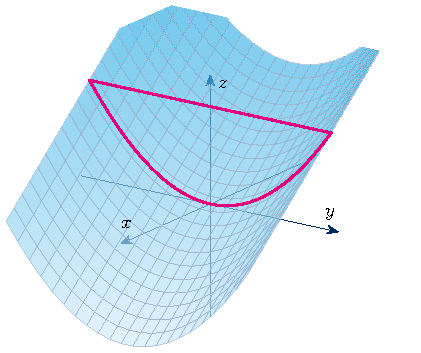
\includegraphics[max width=\linewidth]{Fig11.pdf}
\caption{El gráfico de $z=\tfrac12 y^2 - x$.}
\label{fig11}
\end{figure}
\begin{figure}[htbp]
\centering
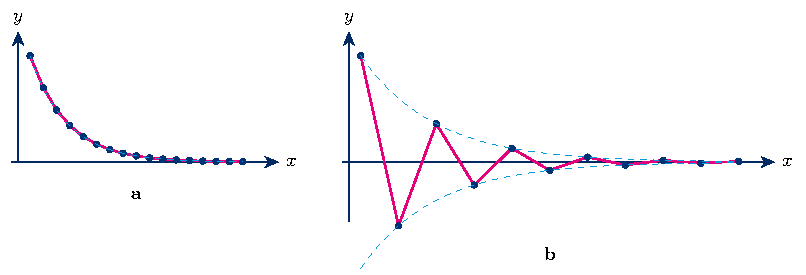
\includegraphics[max width=\linewidth]{Fig12.pdf}
\caption{Iteraciones: {\bf a}. Caso $0<\eta<1$. {\bf b}. Caso $1<\eta<2$.}
\label{fig12}
\end{figure}

\subsection{Efecto de la curvatura y método de Newton}

El método de descenso de gradiente no toma en consideración la curvatura de la superficie $z=f(\xx)$, que está descripta por la matriz Hessiana $Hf(\xx)$.  Necesitaremos algunas propiedades de esta matriz.
\begin{prop}\label{prop.H}
Sea $f\colon D\subset\R^n\to \R$ una función de clase $C^2$. Valen las siguientes propiedades:
\begin{itemize}
\item[(a)] La matriz Hessiana es simétrica;
\item[(b)] Para todo $\xx\in D$, los autovalores de $Hf(\xx)$ son reales;
\item[(c)] Para todo $\xx\in D$, la matriz Hessiana $Hf(\xx)$ es diagonalizable y existe una base ortonormal $\{\uu_i\}_{1\le i\le n}$ de $\R^n$ formada por autovectores de $Hf(\xx)$.
\item[(d)] Dado $\vv\in\R^n$, si definimos $v_i = \vv\cdot\uu_i$, se tiene que
$$
\vv Hf(\xx)\vv^t = \sum_{i=1}^n \lambda_i v_i^2,
$$
donde $\lambda_i$ es el autovalor correspondiente a $\uu_i$ (los $\lambda_i$ son los autovalores de $Hf(\xx)$ contados según su multiplicidad).
\item[(e)] Si llamamos $\lambda_\text{min}$ y $\lambda_\text{max}$ al menor y mayor autovalor de $Hf(\xx)$ respectivamente, entonces
$$
\lambda_\text{min} \|\vv\|^2\le \vv Hf(\xx)\vv^t\le \lambda_\text{max} \|\vv\|^2.
$$
\end{itemize}
\end{prop}
\begin{proof}
Para ver (a), sólo hay que observar que como $f\in C^2$, entonces
$$
\frac{\partial^2 f}{\partial x_i\partial x_j}(\xx) = \frac{\partial^2 f}{\partial x_j\partial x_i}(\xx).
$$
Las propiedades (b)--(e) son propiedades conocidas de matrices simétricas.
\end{proof}

La fórmula \eqref{iteracion2} provee la recurrencia para el método de descenso de gradiente. Observamos que la aproximación lineal
\begin{align*}
f(\xx_{k+1}) &\simeq f(\xx_k) + \nabla f(\xx_k)\cdot (\xx_{k+1}-\xx_k)\\
&= f(\xx_k) - \eta \|\nabla f(\xx_k)\|^2 < f(\xx_k),
\end{align*}
produce un valor de $f$ menor que el valor previo. Pero esto es sólo una aproximación que se verifica al eliminar la corrección cuadrática y funciona para valores pequeños de $\eta$. Si tomamos en consideración los términos cuadráticos, entonces vemos que la desigualdad puede no ser más cierta. Para estudiar este caso, hacemos una aproximación de segundo orden
\begin{align*}
f(\xx_{k+1}) &\simeq f(\xx_k) + \nabla f(\xx_k)\cdot (\xx_{k+1}-\xx_k) + \frac12 (\xx_{k+1}-\xx_k) Hf(\xx_k) (\xx_{k+1}-\xx_k)^t\\
&=  f(\xx_k) - \eta \|\nabla f(\xx_k)\|^2 + \frac{\eta^2}{2} \nabla f(\xx_k) Hf(\xx_k) \nabla f(\xx_k)^t.
\end{align*}
El último término es el término de corrección debido a la curvatura de $f$. Hay dos casos de importancia que vale la pena resaltar:
\begin{enumerate}
\item El Hessiano $Hf$ es definido negativo (en ese caso el punto crítico es un máximo, no un mínimo, así que este caso solo ilustra el signo de la corrección). Entonces el término de corrección es negativo, luego la aproximación de Taylor implica
$$
f(\xx_{k+1}) < f(\xx_k) - \eta \|\nabla f(\xx_k)\|^2 < f(\xx_k),
$$
es decir que para cualquier tasa de aprendizaje $\eta>0$ cada iteración provee un valor de $f$ más pequeño.

\item El Hessiano $Hf$ es definido positivo. En este caso el término de corrección es positivo. La Proposición \ref{prop.H}, parte (e), nos da una cota de error para el término de corrección:
$$
0\le \frac{\eta^2}{2} \lambda_\text{min} \|\nabla f(\xx_k)\|^2 \le \frac{\eta^2}{2}  \nabla f(\xx_k) Hf(\xx_k) \nabla f(\xx_k)^t \le \frac{\eta^2}{2} \lambda_\text{max} \|\nabla f(\xx_k)\|^2.
$$
Luego al comparar los valores de $f$ en iteraciones sucesivas, obtenemos
\begin{align*}
f(\xx_{k+1}) &\simeq f(\xx_k) - \eta \|\nabla f(\xx_k)\|^2 + \frac{\eta^2}{2} \nabla f(\xx_k) Hf(\xx_k) \nabla f(\xx_k)^t\\
&\le f(\xx_k) - \eta \|\nabla f(\xx_k)\|^2 + \frac{\eta^2}{2} \lambda_\text{max} \|\nabla f(\xx_k)\|^2,
\end{align*}
(donde $\lambda_\text{max}$ es el mayor autovalor de $Hf(\xx_k)$; para una cota uniforme se toma el supremo sobre la región que recorren las iteraciones), y este último término es menor que $f(\xx_k)$ si y sólo si
\begin{equation}\label{cota.delta}
-\eta + \frac{\eta^2}{2}\lambda_\text{max} <0 \iff \eta < \frac{2}{\lambda_\text{max}}.
\end{equation}
Luego, si la tasa de aprendizaje verifica \eqref{cota.delta}, entonces la aproximación cuadrática nos da un valor para $f(\xx_{k+1})$ menor que $f(\xx_k)$.

\item El Hessiano $Hf$ es indefinido (punto silla, el caso típico en funciones de costo de redes). El término de corrección puede tener cualquier signo, según la dirección de $\nabla f(\xx_k)$ respecto de los autovectores.
\end{enumerate}
El argumento anterior es heurístico, porque se usa $\simeq$ y luego una desigualdad. Una versión rigurosa es la siguiente.
\begin{lema}[Lema del descenso]\label{lema.descenso}
Sea $f\colon\R^n\to\R$ de clase $C^1$ con $\nabla f$ Lipschitz de constante $L$, es decir, $\|\nabla f(\xx)-\nabla f(\yy)\|\le L\|\xx-\yy\|$. Entonces, para todo $\xx$ y todo $\eta>0$,
$$
f(\xx-\eta\nabla f(\xx))\le f(\xx)-\eta\Bigl(1-\frac{L\eta}{2}\Bigr)\|\nabla f(\xx)\|^2.
$$
En particular, si $0<\eta<2/L$ y $\nabla f(\xx)\ne0$, el valor de $f$ disminuye estrictamente.
\end{lema}
\begin{proof}
Sea $\yy=\xx-\eta\nabla f(\xx)$. Por el teorema fundamental del cálculo,
$$
f(\yy)-f(\xx)=\int_0^1\nabla f(\xx+s(\yy-\xx))\cdot(\yy-\xx)\,ds
=\nabla f(\xx)\cdot(\yy-\xx)+\int_0^1\bigl(\nabla f(\xx+s(\yy-\xx))-\nabla f(\xx)\bigr)\cdot(\yy-\xx)\,ds.
$$
La integral se acota, por Cauchy--Schwarz y la hipótesis, por $\int_0^1 Ls\|\yy-\xx\|^2ds=\frac L2\|\yy-\xx\|^2$. Como $\yy-\xx=-\eta\nabla f(\xx)$, queda $f(\yy)-f(\xx)\le-\eta\|\nabla f(\xx)\|^2+\frac{L\eta^2}{2}\|\nabla f(\xx)\|^2$.
\end{proof}
Si $f$ es de clase $C^2$, la constante $L$ se puede tomar como el supremo de $\lambda_\text{max}$ en valor absoluto de $Hf$, lo que explica la condición \eqref{cota.delta}.

El {\em método de Newton} (o {\em método del Hessiano}) usa la información de curvatura de otra manera: en lugar de \eqref{iteracion2}, cuando $Hf(\xx_k)$ es inversible, itera
$$
\xx_{k+1}=\xx_k-\bigl(Hf(\xx_k)\bigr)^{-1}\nabla f(\xx_k),
$$
que es el punto crítico de la aproximación cuadrática de $f$ en $\xx_k$. Requiere calcular e invertir el Hessiano en cada paso, lo que es muy costoso cuando hay muchos parámetros.

\section{Búsqueda estocástica}\label{sec.c4.3}

El método de descenso de gradiente no provee resultados satisfactorios en todos los casos. Esto puede ser corregido con ciertas variantes del método. Pero, algunas veces es necesario modificar el método para evitar caer en regiones {\em plateau} (donde el gradiente es muy pequeño sin que en esa región se encuentre el mínimo buscado) y el método de descenso se vuelve muy ineficiente. En esta sección presentamos un método que tiene una variante estocástica que soluciona este inconveniente. El mínimo es buscado a lo largo de un procesos de difusión aleatoria en lugar de seguir un camino determinístico. 

\subsection{Modelo determinístico}

Para entender la idea que vamos a utilizar, analicemos primero el modelo determinístico de descenso de gradiente desde otra perspectiva.

Supongamos que elegimos un punto de partida $\xx_0$ y queremos encontrar el camino más rápido para llegar a $\xx^*$, el mínimo de nuestra función $f$. La idea entonces es buscar ese camino $\xx(t)$ como una curva integral de un cierto campo vectorial $\bb(\xx)$, i.e.
$$
\xx'(t) = \bb(\xx(t)),\qquad \xx(0)=\xx_0.
$$
El objetivo entonces es el de encontrar al campo $\bb(\xx)$ de manera tal que la función $\varphi(t) := f(\xx(t))$ decaiga lo más rápidamente posible. Luego, calculamos la derivada de $\varphi(t)$:
$$
\varphi'(t) = \frac{d}{dt}f(\xx(t)) = \nabla f(\xx(t)) \cdot \xx'(t) = \nabla f(\xx(t))\cdot \bb(\xx(t)).
$$
Entre los campos con $\|\bb(\xx)\|$ dado, esta derivada se hace mínima (por Cauchy--Schwarz) si $\bb(\xx) = -\lambda\nabla f(\xx)$ con $\lambda>0$, es decir, si usamos el método de descenso de gradiente.

\subsection{Variante estocástica}

Observemos que en el modelo determinista (descenso de gradiente) si se ingresa en una región en donde el gradiente de $f$ es pequeño, la tasa de cambio de la trayectoria $\xx(t)$ es pequeña, entonces el tiempo que tarda en salir de esa región (asumiendo que el mínimo aún se encuentra lejos) puede ser muy grande. Una manera de solucionar este problema es introducir {\em ruido} o un {\em componente aleatorio}. La idea va a ser que este ruido sea chico en regiones donde el gradiente de $f$ sea grande pero que el ruido aumente si se ingresa a una región de plateau.

Para poder avanzar en la introducción del ruido, veamos primero unos conceptos probabilísticos.

\subsubsection{Movimiento Browniano y ruido blanco}
Vamos a dar una muy breve definición e introducción a este tema. Recomendamos una lectura más detallada del mismo y pueden hacerlo, por ejemplo, en \cite{Dynkin, Evans} o en las notas \cite{Bonder-Groisman}.

\begin{defi}\label{defi.W}
Un movimiento Browniano, o proceso de Wiener, es un proceso estocástico $W_t$, $t\ge 0$, tal que
\begin{enumerate}
\item $W_0=0$ casi seguramente;\label{W1}

\item si $0\le u<s<t$, entonces $W_t-W_s$ y $W_s-W_u$ son independientes (el proceso tiene incrementos independientes);\label{W2}

\item $t\mapsto W_t$ es continuo casi seguramente;\label{W3}

\item los incrementos están normalmente distribuidos, con $W_t-W_s \sim N(0,|t-s|)$.\label{W4}
\end{enumerate}
\end{defi}

Observemos que por \ref{W1} y \ref{W4} tenemos que $\E[W_t] = 0$ y $\E[W_t^2] = t$.

Un movimiento Browniano $m-$dimensional es un vector $W_t = (W_t^1,\dots, W_t^m)$ en donde cada componente $W_t^k$ es un movimiento Browniano dado por la Definición \ref{defi.W} y son independientes.

Sea $\bb\colon \R^n\to\R^n$ un campo vectorial de clase $C^1$ y sea $\sigma\colon \R^n\to\R^{n\times m}$ una matriz de clase $C^1$.

Se define entonces el proceso estocástico $X_t\in \R^n$ como la solución de la ecuación diferencial estocástica
\begin{equation}\label{SDE}
dX_t = \bb(X_t)\, dt + \sigma(X_t)\, dW_t.
\end{equation}
Al campo $\bb(\xx)$ se lo llama la {\em deriva} (en inglés {\em drift}) y a la matriz $\sigma(\xx)$ se la llama {\em difusión} (en inglés {\em diffusion}).

Para entender lo que significa una solución de \eqref{SDE}, es conveniente mirar la ecuación a tiempo discreto. Fijemos un $\delta>0$ y tomemos $t_k = k\delta$. Notemos además $X_k = X_{t_k}$. Entonces \eqref{SDE} se transforma en
$$
X_{k+1}-X_k = \bb(X_k) \delta + \sigma(X_k) (W_{t_{k+1}}-W_{t_k}).
$$
Si usamos la condición \ref{W4} de la Definición \ref{defi.W}, entonces $B_k:= W_{t_{k+1}}-W_{t_k} \sim N(0,\delta I_m)$ (donde $I_m$ es la identidad de $\R^{m\times m}$), luego llegamos a
\begin{equation}\label{SDE.discreta}
X_{k+1} = X_k + \bb(X_k) \delta + \sigma(X_k) B_k.
\end{equation}
(Este esquema se llama el {\em método de Euler-Maruyama} para la aproximación de ecuaciones diferenciales estocásticas) 

Comparemos \eqref{SDE.discreta} con el método de descenso de gradiente \eqref{iteracion2}. Observemos que si tomamos $\bb(\xx)=-\nabla f(\xx)$ lo que tenemos es una perturbación aleatoria del descenso de gradiente.

Razonemos ahora como en la sección previa. Lo que queremos es buscar entonces el campo $\bb(\xx)$ y la matriz de difusión $\sigma(\xx)$ de manera tal que $f(X_t)$ decaiga lo más rápidamente posible. Al ser un objeto aleatorio, lo que se busca es que decaiga {\em en promedio} lo más rápidamente posible. Luego, la cantidad a analizar es 
$$
\varphi(t) = \E[f(X_t)|X_0=\xx_0].
$$

Para analizar la variación de $\varphi(t)$, se usa la {\em fórmula de Dynkin} (ver \cite{Dynkin})
\begin{equation}\label{incremento}
\varphi(t+\delta) = \varphi(t) + \delta \E[\A f(X_t)|X_0=\xx_0] + o(\delta),
\end{equation}
donde
$$
\A f = \sum_{i, j=1}^n a_{ij} \frac{\partial^2 f}{\partial x_i \partial x_j} + \sum_{k=1}^n b_k \frac{\partial f}{\partial x_k} = \text{tr}(A Hf) + \bb\cdot\nabla f.
$$
con 
$$
A=(a_{ij})_{1\le i,j\le n},\ A = \frac12 \sigma \sigma^t \qquad\text{y}\qquad \bb=(b_1,\dots,b_n).
$$

Ahora, cuando la curva se encuentra en el plateau, la función objetivo es plana, luego tiene un Hessiano pequeño. Para poder salir del plateau entonces ahí vamos a definir una matriz de difusión grande. Consecuentemente, elegimos la matriz de difusión $\sigma$ de manera tal que $\sigma\sigma^t$ sea proporcional a la inversa del Hessiano, i.e.
\begin{equation}\label{sigma}
\sigma\sigma^t = \lambda (Hf)^{-1}.
\end{equation}
(Esto requiere que $Hf$ sea definida positiva en cada punto, para que $(Hf)^{-1}$ exista y $\sigma$ pueda definirse; en un plateau, $Hf\to0$ y su inversa crece sin control.)
Con esta elección, obtenemos
$$
\A f(\xx) = \frac{n}{2}\lambda + \nabla f(\xx)\cdot \bb(\xx),
$$
y ahora, para minimizar $\A f(\xx)$ elegimos $\bb(\xx)=-\eta\nabla f(\xx)$, de donde obtenemos
$$
\A f(\xx) = \frac{n}{2}\lambda - \eta\|\nabla f(\xx)\|^2.
$$
Si queremos que $\A f(\xx)<0$ necesitamos que el parámetro de ruido $\lambda$ y la tasa $\eta$ verifiquen la relación
$$
\frac{\lambda}{\eta} < \frac{2}{n} \|\nabla f(\xx)\|^2.
$$
Notemos que en un plateau $\|\nabla f\|\approx0$, de modo que esta condición fuerza a que $\lambda$ sea chico justamente donde se quería ruido grande: el método es un compromiso entre ruido y deriva.
Para poder entender mejor este método, analicemos un ejemplo sencillo,

\begin{ejem}
Consideremos el caso unidimensional dado por la función objetivo $f(x)=\tfrac12 x^2$ para $x\in (a,b)$ con $a>0$. Luego la ecuación estocástica queda $dX_t = b(X_t)\, dt + \sigma(X_t)\, dW_t$, $X_0=x_0\in (a, b)$.

El Hessiano en este caso coincide con la derivada segunda $Hf(x) = f''(x) = 1$, luego debemos elegir 
$$
\sigma\sigma^t = \sigma^2 = \lambda \frac{1}{f''(x)} = \lambda\quad\Rightarrow\quad \sigma=\sqrt{\lambda}.
$$
Por otro lado,
$$
b(x) = -\eta f'(x) = -\eta x.
$$
Ahora $\lambda$ y $\eta$ deben verificar
$$
\frac{\lambda}{\eta} < 2|f'(x)|^2 = 2x^2
$$
como $x\in(a,b)$ podemos elegir $\lambda=2a^2\eta$. La ecuación estocástica queda
$$
dX_t = -\eta X_t\, dt + \sqrt{\lambda}\, dW_t,\qquad X_0=x_0.
$$
Esta ecuación se llama {\em ecuación de Langevin}. La solución a esta ecuación viene dada por el {\em proceso de Ornstein-Uhlenbeck}
$$
X_t = x_0 e^{-\eta t} + \sqrt{\lambda} \int_0^t e^{-\eta(t-s)}\, dW_s,
$$
que es la suma de una función determinística y una integral estocástica.
Ahora observemos que
\begin{equation}\label{esperanzas}
\E\left[\int_0^t h(s)\, dW_s\right] = 0\qquad \text{y}\qquad \E\left[\left(\int_0^t h(s)\, dW_s\right)^2\right] = \int_0^t h^2(s)\, ds.
\end{equation}
Estas igualdades se ven fácilmente recordando que
$$
\int_0^t h(s)\, dW_s \simeq \sum_{k=1}^N h(s_k) \underbrace{(W_{s_k+\delta} - W_{s_k})}_{B_k},
$$
donde $N\delta=t$ y observando que $\E[B_k]=0$, $\E[B_k^2]=\delta$ y $B_k, B_j$ son independientes si $k\neq j$. Ver las propiedades de la Definición \ref{defi.W}.

Usando \eqref{esperanzas}, se llega a
$$
\E[X_t] = x_0e^{-\eta t}\qquad \text{y} \qquad \V[X_t] = \frac{\lambda}{2\eta} (1-e^{-2\eta t}).
$$
La media representa la dirección esperada del movimiento, mientras que la integral es la parte del ruido blanco.

La altura esperada $\varphi(t)$ se puede calcular explícitamente en este caso
\begin{align*}
\varphi(t) & = \E[f(X_t)|X_0=x_0] = \frac12 \E[(X_t)^2|X_0=x_0]\\
&= \frac12 \E\left[ x_0^2 e^{-2\eta t} + 2x_0\sqrt{\lambda}e^{-\eta t}\int_0^t e^{-\eta(t-s)}\, dW_s + \lambda\left(\int_0^t e^{-\eta(t-s)}\, dW_s\right)^2\right]\\
&= \frac12 \left( x_0^2 e^{-2\eta t} +  \frac{\lambda}{2\eta} (1-e^{-2\eta t})\right) = \frac12 \left(\frac{\lambda}{2\eta} + \left(x_0^2 - \frac{\lambda}{2\eta}\right) e^{-2\eta t}\right).
\end{align*}
Como $\frac{\lambda}{2\eta}=a^2<x_0^2$, sigue que $\varphi(t)$ es decreciente, luego el mínimo será
$$
\lim_{t\to\infty} \varphi(t) = \frac12\frac{\lambda}{2\eta} = \frac12 a^2.
$$
Aquí el valor $\frac12a^2$ coincide con $\inf_{(a,b)}f$ por la elección $\lambda=2a^2\eta$ hecha al comienzo. Notemos además que el proceso no respeta la restricción $x\in(a,b)$: el proceso de Ornstein--Uhlenbeck tiene soporte en todo $\R$ y sale del intervalo casi seguramente. El ejemplo ilustra, entonces, solamente el cálculo de $\varphi(t)$.
\end{ejem}

\section{Resumen}\label{sec.c4.4}

Encontrar el mínimo global de una función de costo dada, es un ingrediente importante en cualquier algoritmo de aprendizaje automático. El proceso de aprendizaje es asociado con el proceso de ajustar las variable de la función de costo en sus valores optimales. Algunos métodos son de primer orden (es decir que involucran sólo las derivadas primeras), como por ejemplo el método de descenso de gradiente lo que los hace eficientes computacionalmente. Algunos otros métodos son de segundo orden e involucran las derivadas segundas, como por ejemplo el método del Hessiano.

El más conocido y utilizado de los métodos para minimización es el de descenso de gradiente. Este método es fácil de implementar, pero presenta dificultades cuando la función de costo no es convexa. Este método se puede mejorar de varias maneras para evitar caer en mínimos locales o en zonas de plateau. En estas notas sólo discutimos unas pocas variantes, pero pueden consultar en \cite{Calin} por más variantes como AdaGrad, Adam, AdaMax, RMSProp, por ejemplo.

La búsqueda estocástica propone un algoritmo para salir de las zonas de plateau. Esto involucra la búsqueda de mínimos a lo largo de procesos estocásticos en lugar de curvas determinísticas. Este método, sin embargo, resulta computacionalmente costoso dado que involucra el cálculo de la inversa de la matriz Hessiana de la función de costo.

\section{Ejercicios}\label{sec.c4.5}

\begin{ejer}
Sea $f(x, y) = e^x\sin y$, con $(x, y)\in (0,1)\times (0,\tfrac{\pi}{2})$.
\begin{itemize}
\item[(a)] Mostrar que $f$ es armónica (i.e. $f_{xx} + f_{yy} = 0$);

\item[(b)] Hallar $\|\nabla f\|$;

\item[(c)] Mostrar que la ecuación $\nabla f=0$ no posee soluciones;

\item[(d)] Hallar los máximos y mínimos de $f$ (como el dominio es abierto, pueden no alcanzarse: hallar el supremo y el ínfimo).
\end{itemize}
\end{ejer}

\begin{ejer}
Considerar la forma cuadrática $Q(\xx) = \frac12 \xx A \xx^t - \bb\cdot\xx$, donde $A\in\R^{n\times n}$ es una matriz simétrica no singular.
\begin{itemize}
\item[(a)] Hallar el gradiente $\nabla Q$;

\item[(b)] Escribir la iteración de descenso de gradiente;

\item[(c)] Hallar el Hessiano $HQ$;

\item[(d)] Escribir la iteración del método de Newton.
\end{itemize} 
\end{ejer}


%%%%%%%%%%%%%%%%%%%%%%%%%%%%%%%%%%%%%%%%
%% CAPITULO 5 %%%%%%%%%%%%%%%%%%%%%%%%%%%%%%%
%%%%%%%%%%%%%%%%%%%%%%%%%%%%%%%%%%%%%%%%

\chapter{Neuronas abstractas}\label{cap5}

El concepto de {\em neuronas abstractas} es el componente fundamental de cualquier red neuronal. Es una unidad que imita el comportamiento de una neurona biológica y consiste de una entrada (señal de entrada), pesos (pesos sinápticos) y una función de activación (modelo de disparo neuronal). Este capítulo introduce los tipos más comunes de neuronas (perceptrones, neuronas sigmoides, etc.) e investiga sus propiedades.

Se define la neurona abstracta (Sección~\ref{sec.c5.1}) y se estudian sus casos principales: el perceptrón (Sección~\ref{sec.c5.2}), la neurona sigmoide (Sección~\ref{sec.c5.3}) con su aplicación a la regresión logística (Sección~\ref{sec.c5.4}), las neuronas lineales (Sección~\ref{sec.c5.5}) y la neurona de entrada continua (Sección~\ref{sec.c5.6}). Corresponde al Capítulo~5 de~\cite{Calin}.

\section{Definición y propiedades}\label{sec.c5.1}

En vista de los ejemplos presentados en el Capítulo \ref{cap1}, consideremos la siguiente definición que formaliza la intuición desarrollada:

\begin{defi}
Una neurona abstracta es un cuádruple $(\xx, \ww, \varphi, y)$, donde $\xx = (x_0,\dots, x_n)$ es el vector de entrada, $\ww=(w_0,\dots,w_n)$ es el vector de pesos, con $x_0=1$ y $w_0=b$, el sesgo, y $\varphi$ es la función de activación que define la función de salida $y=\varphi(\ww\cdot \xx)=\varphi(\sum_{i=0}^n w_ix_i)$.
\end{defi}

La forma en que una neurona abstracta aprende un objetivo deseado $\zz$ es ajustando los pesos $\ww$ de manera tal que una cierta función que mide el error entre las variables deseadas $\zz$ y las salidas $y$ sea minimizada. Algunas posibles funciones de error las hemos visto en el Capítulo \ref{cap3} y los algoritmos de minimización los tratamos en el Capítulo \ref{cap4}.

La neurona abstracta está representada en la Figura \ref{fig13}. La unidad de cómputo está dividida en dos partes: la primera contiene el símbolo de sumación, $\sum$, que indica la suma de las entradas con los pesos respectivos, y la segunda contiene a la función de activación $\varphi$ usada para definir la salida $y$.

\begin{figure}[htbp]
\centering
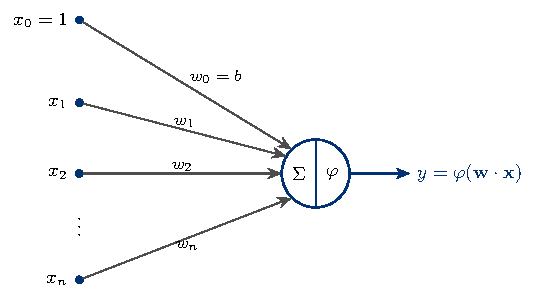
\includegraphics[max width=\linewidth]{Fig13.pdf}
\caption{Una neurona abstracta con sesgo $b$ y función de activación $\varphi$.}
\label{fig13}
\end{figure}

Notemos que el sesgo $b$ está incluido en el sistema de pesos $w_0=b$ con entrada constante $x_0=1$. La expresión del producto interno es entonces
$$
\ww\cdot \xx = w_1 x_1 + \cdots + w_n x_n + b.
$$
A los vectores $\ww = (w_0,\dots,w_n)$ y  $\xx = (x_0,\dots, x_n)$ se los llaman los vectores de {\em pesos extendidos} y de {\em entradas extendidas} respectivamente. La función de salida $y=\varphi(\ww\cdot\xx)$ se la llama también la {\em función primitiva} de la unidad de cómputo.

Las entradas $\{x_i\}_{i=1,\dots, n}$ son comunicadas a través de ejes a la unidad de cómputo luego de ser previamente multiplicadas por los pesos, ver Figura~\ref{fig13}. Los datos de entrada pueden ser de diversos tipos, como por ejemplo:
\begin{itemize}
\item {\em binario} si $x_i\in \{0, 1\}$ para $i=1,\dots, n$;

\item {\em signo} si $x_i\in \{-1, 1\}$ para $i=1,\dots, n$;

\item {\em dígito} si $x_i\in \{0, 1, 2, 3, 4, 5, 6, 7, 8, 9\}$ para $i=1,\dots, n$;

\item {\em números reales arbitrarios} si $x_i\in \R$ para $i=1,\dots, n$;

\item {\em números reales acotados} si $x_i\in [a, b]$ para $i=1,\dots, n$.
\end{itemize}
Por ejemplo, todo dígito escrito a mano puede ser transformado en un dato digital, ver Figura~\ref{fig14}. La matriz de $4\times 4$ se lee línea a línea y se ubica como una sucesión de 0s y 1s de longitud 16. Se pone un valor de 1 si el pixel asignado es activado en más del un 50\%. De otra forma se asigna el valor 0. Codificar caracteres de esta manera es muy simplista y se pierde información sobre formas locales. Sin embargo hay mejores maneras de codificar figuras usando {\em convoluciones}. En general, en el caso de imágenes en escala en grises, cada píxel tiene una activación que es un número entre 0 y 1 (1 para negro y 0 para blanco).

\subsection*{Digresión: eficiencia de la entrada} (Este argumento, de ingeniería de circuitos, no se usa en el resto del curso.) Asumamos que uno quiere implementar un circuito de neuronas. Una pregunta que debe ser hecha es: ¿qué tipo de datos es más eficiente? Equivalentemente, ¿cuántos cambios de estado optimizan la información transmitida desde el punto de vista del costo de circuito de implementación?

\begin{figure}[htbp]
\centering
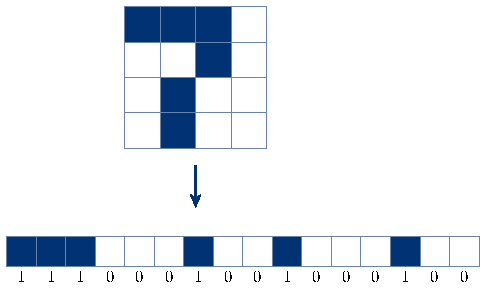
\includegraphics[max width=\linewidth]{Fig14.pdf}
\caption{La transformación de $4\times 4$ píxeles en una sucesión de 0s y 1s.}
\label{fig14}
\end{figure}

Para responder a esta pregunta, sea $\beta$ el número de estados de la señal de entrada, por ejemplo $\beta=2$ para señales binarias. El número de canales o entradas viene dado por $n$. El costo de implementación, $F$, se asume (como modelo simplificado) proporcional tanto con $n$ como con $\beta$, i.e. $F=cn\beta$ donde $c>0$ es la constante de proporcionalidad. Usando $n$ canales con $\beta$ estados, nos da un total de $\beta^n$ entradas posibles. Asumamos ahora que el costo $F$ es fijo y tratemos de optimizar la cantidad de números transmitidos como función de $\beta$. Consideremos la constante $k=\tfrac{F}{c}$, entonces $n=\tfrac{F}{c\beta} = \tfrac{k}{\beta}$. Entonces el número de entradas totales representadas es $f(\beta) = \beta^n = \beta^{\frac{k}{\beta}}$. Para calcular el máximo de esta función, tomamos el logaritmo (que es una función monótona) $g(\beta) = \ln f(\beta) = \tfrac{k}{\beta} \ln \beta$ y su derivada es $g'(\beta)=\tfrac{k}{\beta^2}(1-\ln \beta)$. En consecuencia, el máximo se alcanza para $\beta=e\simeq 2.718$. El entero más próximo a este número es 3, por ende $\beta=3$ es el número óptimo de estados para las señales de entrada desde el punto de vista del costo. 

Sin embargo, este no es el único punto de vista y nos centraremos en una teoría de modelos de neuronas con cualquier número de estados para las señales de entrada.

En lo que sigue presentaremos algunos tipos clásicos de neuronas especificando sus tipos de entradas y funciones de activación.

\section{El modelo del perceptrón}\label{sec.c5.2}

Un {\em perceptrón} es una neurona cuya entrada es cero o uno, i.e. $x_i\in \{0, 1\}$ , y cuya función de activación viene dada por la función de Heaviside
$$
\varphi(x) = \begin{cases}
1,& \text{si } x\ge 0\\
0,& \text{si } x< 0.
\end{cases}
$$
La salida del perceptrón es una {\em puerta umbral}
$$
y=\varphi(\ww\cdot \xx + b) = \begin{cases}
1,& \text{si } \sum_{i=1}^n w_i x_i \ge -b\\
0,& \text{si } \sum_{i=1}^n w_i x_i < -b.
\end{cases}
$$
De esta manera, un perceptrón es una regla que toma decisiones pesando la evidencia dada por las entradas $\{x_i\}_{i=1,\dots,n}$. El umbral $-b$ es una medida de qué tan difícil es para el perceptrón decidir que la salida es 1 (cuanto más chico es $-b$, es decir, cuanto mayor es el sesgo $b$, más fácil es). Para todo propósito general, el sesgo es visto como otro peso, denotado por $w_0$.

Veamos la interpretación geométrica del perceptrón. Consideremos un hiperplano $(n-1)-$dimensional en $\R^n$ definido por
$$
\Hc = \{\xx\in\R^n\colon \ww\cdot\xx = -b\},
$$
donde $\xx = (x_1,\dots,x_n)$ y $\ww=(w_1,\dots,w_n)$. El vector normal $\n$ es el vector de pesos $\n=\ww$. El hiperplano para por un punto $\pp$ si se verifica la relación $b=-\ww\cdot\pp$. Luego el resultado $y$ del perceptrón es asociar el valor 0 a uno de los dos semiespacios determinados por el hiperplano $\Hc$ y 1 al resto. Ver Figura~\ref{fig15}. En resumen, dado un borde lineal entre dos regiones, un perceptrón puede determinar a cual región pertenece un punto dado.

\begin{figure}[htbp]
\centering
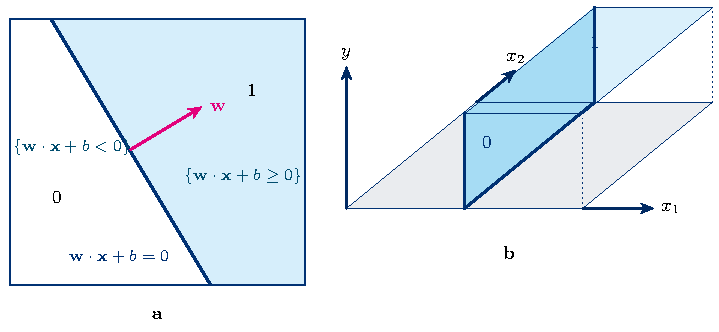
\includegraphics[max width=\linewidth]{Fig15.pdf}
\caption{{\bf a.} La separación del plano en semiespacios. {\bf b.} El gráfico de la función de activación para un perceptrón con dos entradas, $x_1$ y $x_2$.}
\label{fig15}
\end{figure}

El perceptrón puede implementar las puertas lógicas AND ("$\wedge$") y OR ("$\vee$"). Esta propiedad hace importante al perceptrón para cálculos lógicos.

\subsection*{Implementando AND} Consideremos la operación Booleana definida por la tabla
\begin{center}
\begin{tabular}{|c|c|c|}
\hline
$x_1$ & $x_2$ & $y=x_1\wedge x_2$\\ \hline
0 & 0 & 0\\
0 & 1 & 0\\
1 & 0 & 0\\
1 & 1 & 1\\
\hline
\end{tabular}
\end{center}

La misma función de salida $y=x_1\wedge x_2$ puede ser generada por un perceptrón con dos entradas $x_1, x_2\in \{0, 1\}$, pesos $w_1, w_2 = 1$, sesgo $b=-1.5$ y $x_0=1$, ver Figura~\ref{fig16} {\bf a}. La salida se escribe como 
$$
y=\varphi(x_1+x_2 - 1.5) = \begin{cases}
0, & \text{si } x_1+x_2<1.5\\
1, & \text{si } x_1+x_2\ge 1.5
\end{cases}
$$

La condición $\{x_1+x_2\ge 1.5\}$ sólo se satisface si $x_1=x_2=1$, en todos los otros casos se verifica $\{x_1+x_2< 1.5\}$.

En vista de la interpretación geométrica del perceptrón, la linea $x_1+x_2=1.5$ divide los datos de entrada $\{(0,0); (0,1); (1,0); (1,1)\}$ en dos clases asociando 1 al semiespacio $\{x_1+x_2\ge 1.5\}$ y 0 al semiespacio $\{x_1+x_2< 1.5\}$. Ver Figura~\ref{fig17} {\bf a}.

\begin{figure}[htbp]
\centering
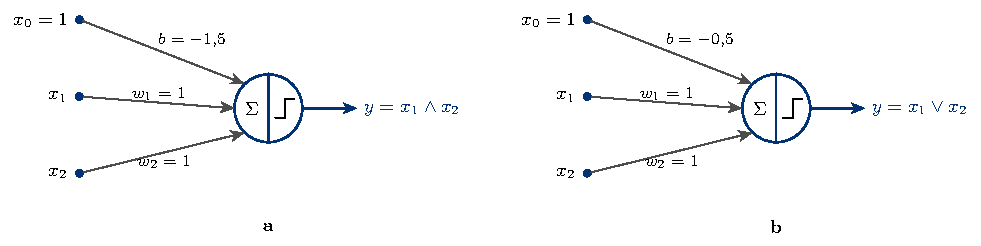
\includegraphics[max width=\linewidth]{Fig16.pdf}
\caption{Implementación de una función Booleana usando un perceptrón: {\bf a.} La función AND. {\bf b.} La función OR.}
\label{fig16}
\end{figure}

\begin{figure}[htbp]
\centering
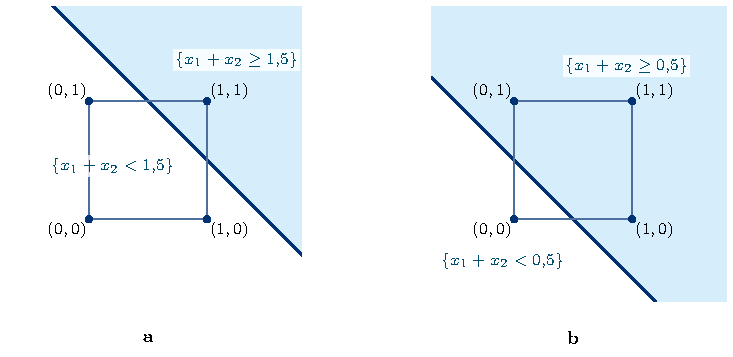
\includegraphics[max width=\linewidth]{Fig17.pdf}
\caption{Partición usando un perceptrón; el semiespacio sombreado es asociado con el valor de salida 1.: {\bf a.} La función AND. {\bf b.} La función OR.}
\label{fig17}
\end{figure}

\subsection*{Implementando OR} Esta función Booleana está definida por la tabla:
\begin{center}
\begin{tabular}{|c|c|c|}
\hline
$x_1$ & $x_2$ & $y=x_1\vee x_2$\\ \hline
0 & 0 & 0\\
0 & 1 & 1\\
1 & 0 & 1\\
1 & 1 & 1\\
\hline
\end{tabular}
\end{center}

La función de salida $y=x_1\vee x_2$ es generada por un perceptrón con dos entradas $x_1, x_2\in \{0,1\}$, pesos $w_1, w_2=1$, sesgo $b=-0.5$ y $x_0=1$, ver Figura~\ref{fig16} {\bf b}. La salida se escribe como
$$
y=\varphi(x_1+x_2 - 0.5) = \begin{cases}
0, & \text{si } x_1+x_2<0.5\\
1, & \text{si } x_1+x_2\ge 0.5.
\end{cases}
$$
La conclusión sigue de la observación de que la condición $\{x_1+x_2<0.5\}$ se satisface si y sólo si $x_1=x_2=0$. Ver la Figura~\ref{fig17} {\bf b} para la interpretación geométrica de este hecho.

Sin embargo, un perceptrón no puede implementar todas las funciones lógicas. Por ejemplo, no puede implementar la función XOR (el OR exclusivo), que viene dado por la tabla
\begin{center}
\begin{tabular}{|c|c|c|}
\hline
$x_1$ & $x_2$ & $y$\\ \hline
0 & 0 & 0\\
0 & 1 & 1\\
1 & 0 & 1\\
1 & 1 & 0\\
\hline
\end{tabular}
\end{center}

Este hecho fue observado por primera vez por Minsky y Papert~\cite{Minsky}. Veremos en el Capítulo~\ref{cap6} que la función XOR puede ser aprendida por una red neuronal de tres perceptrones (dos en una capa oculta y uno de salida).

La imposibilidad de implementar XOR por un perceptrón sigue del hecho que no hay una línea que separe los símbolos 0 y 1 en la Figura \ref{fig18} {\bf a}. Esto puede demostrarse de varias maneras:
\begin{enumerate}
\item Una demostración sigue como consecuencia de las propiedades de separación del plano. Si uno asume por contradicción la existencia de una línea de separación, entonces el plano es dividido por la línea en dos semiplanos, $H_1$ y $H_2$ que son conjuntos convexos (ver Figura \ref{fig18} {\bf b}). Dado que ambos símbolos 1 pertenecen a $H_1$, entonces por convexidad el segmento que los une queda contenido en $H_1$. Análogamente el segmento que une los símbolos 0 es contenido en $H_2$. Como $H_1\cap H_2=\emptyset$, los segmentos que unen los símbolos 1 y 0 deben ser disjuntos, pero esto es una contradicción dado que se intersectan (ver Figura \ref{fig18} {\bf a}).

\item La segunda prueba se basa en motivos algebraicos. Supongamos que un perceptrón $y=\varphi(w_1x_1+w_2x_2+ b)$ implementa XOR. Evaluando en los cuatro puntos: $(0,0)\mapsto0$ da $b<0$; $(1,1)\mapsto0$ da $w_1+w_2+b<0$; $(1,0)\mapsto1$ da $w_1+b\ge0$; y $(0,1)\mapsto1$ da $w_2+b\ge0$. Sumando las dos últimas, $w_1+w_2+2b\ge0$, y junto con $w_1+w_2+b<0$ resulta $b>0$ (restando), lo que contradice $b<0$.
\end{enumerate}

\begin{figure}[htbp]
\centering
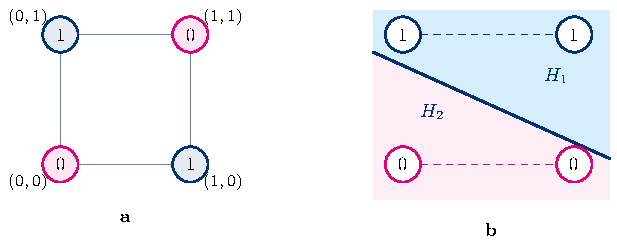
\includegraphics[max width=\linewidth]{Fig18.pdf}
\caption{Clasificación de clústeres usando un perceptrón: {\bf a.} La función XOR. {\bf b.} Una línea divide el plano en dos conjuntos convexos $H_1$ y $H_2$.}
\label{fig18}
\end{figure}

\subsection*{División de clústeres} Motivados por la aplicación previa de división de datos de entrada en clases, lo extendemos al problema más general de clasificación en dos clústeres. Permitimos ahora que los datos de entrada sean números tomando valores en el intervalo $[0,1]$ y asumimos por simplicidad que $n=2$. Entonces cada dato es un par de números reales que se representan como un punto en el cuadrado unitario $[0,1]\times [0,1]$. Supongamos ahora que asociamos una etiqueta o característica con dos posibles valores a cada punto, dada por `grupo 1' (o, color rojo, forma de estrella, etc.) y `grupo 2' (o, color azul, forma de disco, etc.). La pregunta entonces es: ¿puede un perceptrón decidir si un punto dado perteneces a un grupo o al otro? La respuesta va a depender de la distribución de los datos. Si los datos pueden ser separados por una línea de manera tal que un grupo quede contenido en un semiplano y el otro en el otro semiplano, entonces el perceptrón podrá eventualmente ser capaz de decidir qué grupo está asociado con qué etiqueta luego de un adecuado ajuste de los pesos. Para poder hacer esto, introducimos la función
$$
z(x_1, x_2) = \begin{cases}
0, & \text{si } (x_1, x_2)\in \G_1\\
1, & \text{si } (x_1, x_2)\in \G_2,
\end{cases}
$$
donde $\G_1$ y $\G_2$ representan a ``grupo 1'' y ``grupo 2'' respectivamente. El perceptrón decide entre estos dos grupos si somos capaces de encontrar dos pesos $w_1, w_2$ y un sesgo $b$ tales que la línea $w_1 x_1 + w_2 x_2 + b=0$ separa a los grupos $\G_1$ y $\G_2$. Si esto es posible, la función de salida
$$
y=\varphi(w_1 x_1 + w_2 x_2 + b)
$$
tendrá la misma expresión que la dada para la función $z$. Los algoritmos de aprendizaje para el perceptrón (como la regla de Rosenblatt) aparecen en los ejercicios al final del capítulo.

\begin{ejem}
Consideremos la entrada $(x_1, x_2)$, donde $x_1$ denota el talle del calzado y $x_2$ la altura (en pulgadas) de algunas personas en la población. Asociamos una etiqueta para cada individuo considerando el mapa $(x_1,x_2)\mapsto \ell \in \{\text{varón}, \text{mujer}\}$. Dado un par $(x_1, x_2)$, un perceptrón es capaz de distinguir si corresponde a un varón o a una mujer si hay una línea de separación $w_1 x_1 + w_2 x_2 + b=0$ entre los dos grupos.

\begin{figure}[htbp]
\centering
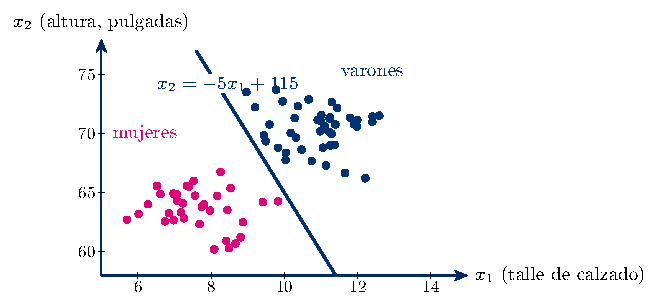
\includegraphics[max width=\linewidth]{Fig19.pdf}
\caption{Clasificación de un perceptrón entre varones y mujeres. La línea $x_2=-5x_1+115$ es un borde de decisión en el espacio $\{x_1, x_2\}$ entre dos clústeres separables linealmente.}
\label{fig19}
\end{figure}

Consideremos datos de talle de calzado y altura de una población de estudiantes (datos sintéticos, generados para ilustrar la idea; en \cite{Calin} se usa un conjunto de datos real) graficados en la Figura \ref{fig19}. Notamos que los grupos de varones y mujeres son separables linealmente con la línea dada por $x_2 = -5 x_1 + 115$. Luego, dado un tamaño de calzado $s$ y una altura $h$, el perceptrón lo clasificará como ``varón'' si $h>-5s + 115$ y como ``mujer'' en caso contrario.

Este problema se puede formular en términos de neuronas de varias maneras
\begin{enumerate}
\item Primero, asociamos un valor numérico a los datos. Etiquetamos los puntos correspondientes a varones como $z=1$ y a los correspondientes a mujeres como $z=-1$. Consideramos la neurona con entrada $(x_1, x_2)$, pesos $w_1, w_2$ y sesgo $b$ teniendo la función de activación
$$
S(u) = \begin{cases}
1, &\text{si } u\ge 0\\
-1, &\text{si } u<0.
\end{cases}
$$
La salida de la neurona será la función $y=S(w_1 x_1 + w_2 x_2 + b)$, ver la Figura~\ref{fig20} {\bf a}. Si $(x_1, x_2)$ corresponde a un varón, entonces $w_1 x_1 + w_2 x_2 + b>0$, y entonces la salida es $y=1$. Si $(x_1, x_2)$ corresponde a una mujer, entonces $w_1 x_1 + w_2 x_2 + b<0$, entonces la salida es $y=-1$. Los parámetros de la línea de separación se obtienen minimizando la función distancia entre la salida y los vectores de etiquetas como
$$
(w_1^*, w_2^*, b^*) = \argmin_{(w_1, w_2, b)} \|\yy-\zz\|^2,
$$
con 
$$
\|\yy - \zz\|^2 = \sum_{\xx\sim \text{datos}}(y(\xx)-z(\xx))^2,
$$
donde $z(\xx)$ e $y(\xx)$ son, respectivamente, las etiquetas y las salidas de los datos $\xx=(x_1, x_2)$. Notemos que, con la activación escalón $S$, la función $(w_1,w_2,b)\mapsto\|\yy-\zz\|^2$ es constante a trozos, con gradiente nulo en casi todo punto, de modo que {\em no} se puede minimizar por descenso de gradiente. Se usa en su lugar la regla de aprendizaje de Rosenblatt (ver los ejercicios), o bien se reemplaza $S$ por una activación suave, como en la Sección~\ref{sec.c5.3}.

\begin{figure}[htbp]
\centering
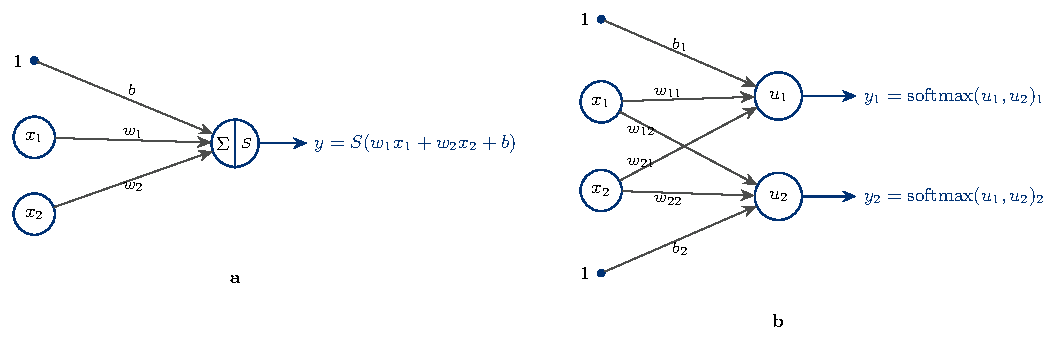
\includegraphics[max width=\linewidth]{Fig20.pdf}
\caption{{\bf a}. La neurona con etiquetas $z\in\{-1, 1\}$. {\bf b}. La red neuronal en el caso de etiquetas en vectores {\em one-hot}.}
\label{fig20}
\end{figure}

\item En este caso usaremos datos etiquetados usando vectores {\em one-hot}. Asociamos el vector $(1, 0)$ con varones y $(0,1)$ con mujeres. Consideramos una red neuronal con entrada $\xx=(x_1, x_2)$ y dos neuronas con función de activación softmax:
$$
(y_1, y_2) = \softmax(u_1, u_2) = \left(\frac{e^{u_1}}{e^{u_1} + e^{u_2}}, \frac{e^{u_2}}{e^{u_1} + e^{u_2}}\right),
$$
ver Figura~\ref{fig20} {\bf b}. Acá, $u_1, u_2$ son las señales tomadas de las entradas como
\begin{align*}
u_1 &= w_{11} x_1 + w_{21} x_2 + b_1\\
u_2 &= w_{12} x_1 + w_{22} x_2 + b_2.
\end{align*}
La función costo a ser minimizada en este caso es
$$
\sum_{\xx\sim\text{datos}} \left((y_1(\xx) - z_1(\xx))^2 + (y_2(\xx) - z_2(\xx))^2\right).
$$
(Con salidas softmax lo natural es usar, en cambio, la entropía cruzada de la Sección~\ref{sec.c3.2}.)
\end{enumerate}
\end{ejem}

\section{La neurona sigmoide}\label{sec.c5.3}

Hemos visto que un perceptrón funciona como una herramienta que provee de dos estados de decisión, 0 y 1, sin valores intermedios. La situación puede ser mejorada si permitimos que la neurona tome valores intermedios en el intervalo $(0,1)$; de esta forma, las salidas cercanas a 1 corresponden a decisiones que son más proclives de ocurrir, mientras que salidas más cercanas a 0 representan decisiones con menor chance de suceder. En este caso, la salida de la neurona ocurre como una medida de verosimilitud para tomar decisiones.

Una {\em neurona sigmoide} es una unidad de cómputo con entrada $\xx=(x_1,\dots,x_n)$ y función de activación dada por la función logística
$$
\sigma(z) = \frac{1}{1+e^{-z}}.
$$
Notamos por $\ww = (w_1,\dots,w_n)$ al vector de pesos y por $b$ al sesgo. La salida de la neurona es un número entre 0 y 1 dado por
$$
y=\sigma(\ww\cdot\xx + b) = \frac{1}{1+e^{-\ww\cdot\xx - b}}.
$$
Si consideramos como función de activación a la función logística escalada
$$
\sigma_c(z) = \frac{1}{1+e^{-cz}},\qquad c>0,
$$
entonces la salida de la neurona sigmoide tiende a la salida del perceptrón cuando $c\to\infty$ (para todo $\xx$ fuera del hiperplano $\ww\cdot\xx=b$).

La ventaja de este tipo de neuronas es doble: Por un lado aproxima perceptrones y por otro la función de salida es continua con respecto a los pesos. Esto último no sucede con los perceptrones. Esta propiedad de continuidad es de extrema importancia en varios algoritmos que veremos más adelante.

Vale la pena notar la forma en que los pesos $w_i$ se relacionan con las entradas $x_i$ y la salida $y$. Para eso usamos la fórmula de la inversa de la función logística, $\sigma^{-1}(t) = \ln\tfrac{t}{1-t}$ para $t\in(0,1)$. Luego la relación $y=\sigma(\ww\cdot\xx + b)$ se convierte en $\ln\tfrac{y}{1-y} = \ww\cdot\xx + b$. Evaluemos ahora esta expresión en dos valores diferentes de los ingresos $x_i = x_i^*$ y $x_i=x_i^*+1$:
\begin{align*}
\ln\frac{y}{1-y} |_{x_i=x_i^*} & = w_1 x_1 + \cdots + w_i x_i^* + \cdots + w_n x_n + b,\\
\ln\frac{y}{1-y} |_{x_i=x_i^*+1} & = w_1 x_1 + \cdots + w_i (x_i^*+1) + \cdots + w_n x_n + b.\\
\end{align*}
Restando ambas expresiones y usando las propiedades del logaritmo llegamos a la expresión
$$
w_i = \ln\left(\frac{\frac{y}{1-y}|_{x_i=x_i^*+1}}{\frac{y}{1-y}|_{x_i=x_i^*}}\right),
$$
(el logaritmo del cociente de las {\em chances} $y/(1-y)$, o {\em log-odds ratio}), que es una expresión independiente de $x_i^*$. Esta expresión permite obtener el valor de los pesos $w_i$ de la neurona en términos de las salidas, si las entradas  se modifican en una unidad.

Una neurona sigmoide puede también tener otras funciones de activación que tengan un aspecto similar, como la tangente hiperbólica $\tb(z) = \tanh z = \tfrac{e^z - e^{-z}}{e^z + e^{-z}}$.

Si bien diferentes elecciones de función sigmoide pueden tener distintas velocidades de aprendizaje, desde el punto de vista matemático tienen un tratamiento muy similar. Por ejemplo, el cambio infinitesimal en la salida de una neurona sigmoide $y=\varphi(\ww\cdot\xx + b)$, con función de activación $\varphi$ en términos de los pesos y sesgo es dada por la expresión diferencial
\begin{align*}
dy &= \sum_{i=1}^n \frac{\partial y}{\partial w_i} dw_i + \frac{\partial y}{\partial b} db\\
&= \sum_{i=1}^n \varphi'(\ww\cdot\xx+ b) x_i dw_i + \varphi'(\ww\cdot\xx+ b) \, db\\
&=\varphi'(\ww\cdot\xx+ b)\left(\sum_{i=1}^n x_i dw_i + db\right).
\end{align*}
Notemos que la variación $dy$ es proporcional a $\varphi'$. Esa constante de proporcionalidad depende de la función sigmoide elegida y en algunos casos es fácilmente calculable. Por ejemplo
\begin{align*}
&\text{si }\varphi(z) = \sigma(z) \quad \text{ entonces } \quad \varphi'(z) = \sigma'(z) = \sigma(z)(1-\sigma(z)),\\
&\text{si }\varphi(z) = \tb(z) \quad \text{ entonces } \quad \varphi'(z) = \tb'(z) = 1-\tb^2(z).
\end{align*}
La expresión diferencial, en términos de los gradientes se expresa como
$$
\nabla y = (\nabla_\ww y, \partial_b y) = \varphi'(\ww\cdot\xx + b) (\xx, 1).
$$
Es decir, el gradiente $\nabla y$ es proporcional al vector extendido de entradas $(\xx, 1)$ con constante de proporcionalidad dada por la derivada de la función de activación $\varphi$. Usaremos este hecho en el {\em algoritmo de retropropagación} (back-propagation algorithm) más adelante.

\section{Regresión logística}\label{sec.c5.4}

En esta sección veremos dos aplicaciones de la neurona sigmoide que aprende usando una {\em regresión logística}. El primer ejemplo trata con pronosticar la probabilidad de default de una compañía y el segundo con una clasificación binaria en clústeres. 

\subsection{Probabilidad de default de una compañía}
Estamos interesados en predecir la probabilidad de default de una compañía durante un cierto período de tiempo $[0, T]$ usando una neurona sigmoide. Asumamos que la entrada $\xx$ de la neurona es un vector que contiene cierta información de la misma como, por ejemplo: Reservas de efectivo, ingresos, costos, gastos de mano de obra, etc. El conjunto de entrenamiento consiste en $n$ pares $\{(\xx_i, z_i)\}_{1\le i\le n}$, con $\xx_i$ como antes y $z_i\in \{-1,1\}$. Un valor $z_i=1$ significa que la $i-$ésima compañía entró en default en el período $[0,T]$ y un valor $z_i=-1$ significa que no entró en default. Las mediciones $\{(\xx_i, z_i)\}_{1\le i\le n}$ representan empíricamente un par de variables aleatorias $(X, Z)$ donde $Z$ toma valores $\pm1$ y $X$ es un vector aleatorio $m-$dimensional. La probabilidad condicional $\P(Z|X)$ viene dada por la tabla
\begin{center}
\begin{tabular}{|c|c|c|}
\hline
$z$ & $-1$ & $1$\\ \hline
$\P(z|\xx)$ & $1-h(\xx)$ & $h(\xx)$ \\ \hline
\end{tabular}
\end{center}
para una cierta función $h\colon \R^m\to [0,1]$, donde $m$ es la dimensión de la entrada $X$ (en esta sección $n$ es la cantidad de datos). Una forma conveniente de elegir $h(\xx)$ es usando una función sigmoide
$$
h(\xx) = \sigma(\ww\cdot\xx),
$$
donde, si se desea incluir un sesgo, $\xx$ y $\ww$ son los vectores extendidos.
El producto interno $\ww\cdot\xx$ se interpreta como el {\em puntaje por defecto} de la compañía con la entrada $\xx$. Un puntaje alto implica que el valor de $\sigma(\ww\cdot\xx)$ es cercano a 1, lo que se interpreta como una alta probabilidad de default. Por otro lado, un valor bajo (negativo) del puntaje implica un valor de $\sigma(\ww\cdot\xx)$ cercano a 0, que se interpreta como una baja probabilidad de default.

Observemos que la función sigmoide $\sigma$ verifica $\sigma(-x) = 1-\sigma(x)$, por lo que si $z=-1$,
$$
\sigma(z\ww\cdot\xx) = \sigma(-\ww\cdot\xx) = 1-\sigma(\ww\cdot\xx) = 1-h(\xx),
$$
y si $z=1$,
$$
\sigma(z\ww\cdot\xx) = \sigma(\ww\cdot\xx) = h(\xx),
$$
Luego, la tabla previa se puede escribir como
\begin{center}
\begin{tabular}{|c|c|c|}
\hline
$z$ & $-1$ & $1$\\ \hline
$\P(z|\xx)$ & $\sigma(-\ww\cdot\xx)$ & $\sigma(\ww\cdot\xx)$ \\ \hline
\end{tabular}
\end{center}
La distribución de probabilidad depende entonces de los parámetros $\ww$ y lo consideramos como un modelo de distribución producido por la neurona. El siguiente paso es encontrar los pesos $\ww$ para los cuales el modelo de distribución aproxima de la mejor manera posible a los datos de entrenamiento $\{(\xx_i, z_i)\}_{1\le i\le n}$. Esto lo podemos conseguir eligiendo $\ww$ de manera tal que la verosimilitud de los datos $z_i$ al aproximarse por $y_i$ sea máxima. Asumiendo independencia de los datos, tenemos
\begin{align*}
\ww^* &= \argmax_{\ww} \P(z_1,\dots,z_n | \xx_1,\dots,\xx_n) \\
&= \argmax_{\ww} \prod_{i=1}^n \P(z_i|\xx_i) = \argmax_{\ww} \ln\left(\prod_{i=1}^n \P(z_i|\xx_i)\right)\\
&=\argmax_{\ww} \sum_{i=1}^n \ln \P(z_i|\xx_i) = \argmin_{\ww} \left(-\sum_{i=1}^n \ln \P(z_i|\xx_i)\right)\\
&= \argmin_{\ww} \left(-\frac{1}{n}\sum_{i=1}^n \ln \P(z_i|\xx_i)\right).
\end{align*}
Ahora observemos que
\begin{align*}
-\frac{1}{n}\sum_{i=1}^n \ln \P(z_i|\xx_i) &= -\frac{1}{n}\sum_{i=1}^n \ln \sigma(z_i \ww\cdot \xx_i) = -\frac{1}{n}\sum_{i=1}^n \ln \frac{1}{1+e^{-z_i\ww\cdot\xx_i}}\\
&=\frac{1}{n}\sum_{i=1}^n \ln(1+e^{-z_i\ww\cdot\xx_i}).
\end{align*}
Luego el peso óptimo está dado por
$$
\ww^* = \argmin_\ww \frac{1}{n}\sum_{i=1}^n \ln(1+e^{-z_i\ww\cdot\xx_i}).
$$
Esta función es la {\em entropía cruzada empírica} (Sección~\ref{sec.c3.2}) entre las etiquetas y las probabilidades del modelo. Es convexa: derivando dos veces se obtiene el Hessiano $\frac1n\sum_{i}\sigma(u_i)(1-\sigma(u_i))\,\xx_i\xx_i^t\succeq0$, con $u_i=z_i\ww\cdot\xx_i$ (se usó $z_i^2=1$), que es definido positivo si los $\xx_i$ generan el espacio. Pero atención: si los datos son linealmente separables, es decir, si existe $\ww_0$ con $z_i\ww_0\cdot\xx_i>0$ para todo $i$, entonces $F(t\ww_0)\to0$ cuando $t\to\infty$, mientras que $F>0$ siempre. Luego $\inf F=0$ no se alcanza: el ``$\argmin$'' no existe y los pesos crecen sin cota ($\|\ww\|\to\infty$).

\subsection*{Descenso de gradiente} No se tiene una fórmula exacta para el valor del peso óptimo $\ww^*$, así que lo buscamos aproximar con una sucesión $\ww_j$ usando el método de descenso de gradiente.

Llamemos
$$
F(\ww) =  \frac{1}{n}\sum_{i=1}^n \ln(1+e^{-z_i\ww\cdot\xx_i}),
$$
su gradiente viene dado por
\begin{align*}
\nabla F(\ww) &= -\frac{1}{n}\sum_{i=1}^n \frac{z_i \xx_i e^{-z_i\ww\cdot\xx_i}}{1+ e^{-z_i\ww\cdot\xx_i}} = -\frac{1}{n}\sum_{i=1}^n \frac{z_i\xx_i}{1+e^{z_i\ww\cdot\xx_i}}\\
&= -\frac{1}{n}\sum_{i=1}^n z_i\xx_i \sigma(-z_i\ww\cdot\xx_i)\\
&=\frac{1}{n}\sum_{i=1}^nz_i\xx_i \sigma(z_i\ww\cdot\xx_i) - \frac{1}{n}\sum_{i=1}^nz_i\xx_i.
\end{align*}

Luego, dado un peso inicial $\ww_0$, la sucesión aproximante viene dada por
$$
\ww_{j+1} = \ww_j - \eta\nabla F(\ww_j) = \ww_j + \frac{\eta}{n}\sum_{i=1}^n z_i\xx_i\sigma(-z_i\ww_j\cdot\xx_i), 
$$
donde $\eta>0$ es la tasa de aprendizaje.

Para aplicar este método, asumiendo que tenemos el conjunto de entrenamiento $\{(\xx_i, z_i)\}_{1\le i\le n}$ y si tenemos una nueva entrada $\xx$ describiendo los parámetros de otra compañía queremos entonces evaluar la probabilidad de default de la misma. Entonces la probabilidad deseada se calcula como $h(\xx) = \sigma(\ww^*\cdot\xx)$, donde $\ww^*=\lim_{j\to\infty} \ww_j$.

\subsection{Clasificación binaria}
Esta sección trata sobre el uso de una neurona sigmoide como un {\em clasificador binario}. Esto significa que una neurona sigmoide es entrenada para distinguir entre dos clústeres distintos en el plano en donde se usa nuevamente la regresión logística como algoritmo de aprendizaje.

Asumamos que tenemos dos grupos de puntos en el plano: blancos y negros. Queremos poder dividir los puntos en dos grupos, el clúster de puntos negros denotado por $\G_1$ y el clúster de puntos blancos denotado por $\G_2$. Si $\xx = (x_1, x_2)$ representa las coordenadas de un punto en el plano, consideramos la función objetivo a la función
$$
z(\xx) = \begin{cases}
1,&\text{si } \xx\in \G_1\\
-1, & \text{si } \xx\in \G_2.
\end{cases}
$$
Asumamos que existe una línea de decisión en el plano dada por $w_1 x_1 + w_2 x_2 + b=0$, que intenta dividir los puntos de los clústeres $\G_1$ y $\G_2$. Ver Figura~\ref{fig21}. El objetivo es ajustar los parámetros $w_1, w_2$ y $b$ para que la línea represente la mejor partición de los datos en los distintos clústeres.

\begin{figure}[htbp]
\centering
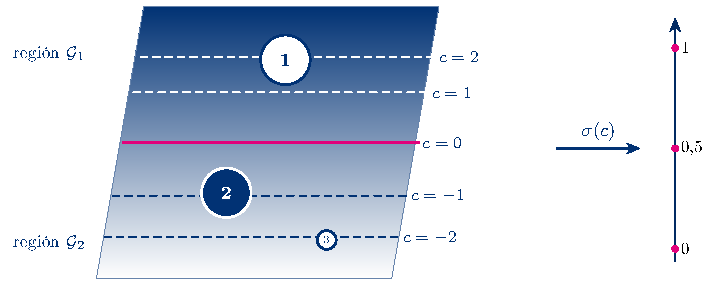
\includegraphics[max width=\linewidth]{Fig21.pdf}
\caption{La familia de líneas $w_1 x_1 + w_2 x_2 + b = c$, $c\in\R$. La función sigmodea $\sigma$ mapea cada línea a un punto en $(0,1)$ visto como una probabilidad.}
\label{fig21}
\end{figure}

Consideremos la partición del plano en líneas paralelas a la línea de decisión 
$$
\{w_1 x_1 + w_2 x_2 + b = c\colon c\in \R\},
$$
ver Figura~\ref{fig21}. Las líneas con valores de $c$ positivo corresponden a la región oscura $\G_1$, mientras que las que tienen un valor negativo de $c$ corresponden a la región $\G_2$. Podemos pensar al plano como una escala de azules desde el blanco, cuando $c=-\infty$, al azul oscuro, cuando $c=+\infty$. 

Cada punto es aproximadamente del mismo color que el color del fondo que lo rodea. Si un punto tiene un color que es muy diferente al fondo en donde está, ese elemento ``sorpresa'' es grande y corresponde a una gran cantidad de información. Por otro lado, si el color del punto no difiere del color de su entorno, entonces la información que provee ese punto es pequeña. Vamos a construir una medida de la información basada en el efecto de esta diferencia de color, que luego será minimizada. La información asociada a un punto $\xx=(x_1, x_2)$ se define como
$$
I(\xx) = -\ln \sigma(z(\xx)(\ww\cdot\xx + b)),
$$
donde $\ww=(w_1, w_2)$. Tratemos de entender esta construcción para los puntos mal clasificados y para los que están correctamente clasificados.

\subsubsection*{El caso de puntos mal clasificados} Elijamos un punto mal clasificado con coordenadas $\xx$. Es decir un punto que tiene un color diferente al de su entorno. Por ejemplo tomemos el punto blanco marcado con ``1'' en la Figura~\ref{fig21} (no confundir esas marcas con las etiquetas $z=\pm1$). Este es un punto blanco en una región muy oscura, por lo que  la información asociada con este evento es grande. Representamos este hecho en la figura considerando un radio grande, de manera tal que la información está asociada al área del disco blanco. Tenemos entonces que existe un $c>0$ tal que $\xx$ verifica $\ww\cdot\xx + b = c$. La función sigmoide $\sigma$ asocia a $c$ con un valor entre 0 y 1 que puede ser considerado como una probabilidad $\P(\xx) = \sigma(c)$. La información asociada con el punto $\xx$ viene dada con la {\em función de verosimilitud negativa logarítmica}, $-\ln \P(\xx) = -\ln \sigma(c)$. Si $c$ es grande, entonces $\sigma(c)$ es próxima a 1, luego la información $-\ln\P(\xx)$ es cercana a 0. Esto no tiene sentido, dado que la información debería ser grande. Para solucionar este problema, definimos la información levemente diferente, usando la probabilidad complementaria. Dado que el punto es blanco, $\xx\in\G_2$, entonces $z(\xx) = -1$. Definimos entonces la probabilidad como $\P(\xx) = \sigma(z(\xx) c)=\sigma(-c) = 1-\sigma(c)$. Luego, cuando $c$ es grande, la probabilidad es cercana a 0, por ende la información $-\ln\P(\xx) = -\ln\sigma(z(\xx)c) = -\ln\sigma(-c) = -\ln(1-\sigma(c))$ es también grande.

De manera análoga, para el punto oscuro marcado con ``2'' dentro de la región blanca de la Figura~\ref{fig21} va a poseer una información alta.

\subsubsection*{El caso de los puntos correctamente clasificados} Elegimos ahora un punto correctamente clasificado, por ejemplo el punto blanco marcado con ``3'' en la Figura~\ref{fig21} situado en el área blanca. Notamos por $\xx$ a sus coordenadas y $c<0$ a la constante tal que $\ww\cdot\xx+ b=c$. Observemos que si $c$ es grande (en valor absoluto) y asociamos a $\xx$ la probabilidad $\P(\xx) = \sigma(z(\xx) c)$, tenemos en este caso que $z(\xx)=-1$ pues $\xx\in\G_2$, luego $\sigma(z(\xx)c)$ estará cerca de 1, luego su logaritmo estará cerca de 0. 

Ahora estamos en la posición de buscar la mejor línea usando la información como función de error. Este método resulta equivalente al método de máxima verosimilitud. Consideramos $n$ puntos del plano con coordenadas $\xx_i$ y tipo de color $z_i = z(\xx_i)$, $1\le i\le n$. La información total se define como la suma de las informaciones puntuales, es decir
$$
E(\ww, b) = \sum_{i=1}^n I(\xx_i) = -\sum_{i=1}^n \ln \sigma(z_i (\ww\cdot\xx_i + b)). 
$$
La mejor línea de decisión es la que corresponde a los valores $\ww$ y $b$ que minimicen a la información total $E$. Estos valores óptimos están dados por
\begin{align*}
(\ww^*, b^*) &= \argmin_{(\ww, b)} E(\ww, b) = \argmax_{(\ww,b)} \sum_{i=1}^n \ln \sigma(z_i (\ww\cdot\xx_i + b))\\
&= \argmax_{(\ww, b)} \ln\left(\prod_{i=1}^n \sigma(z_i (\ww\cdot\xx_i + b))\right)\\
&= \argmax_{(\ww, b)} \ln\left(\prod_{i=1}^n \P_{\ww, b} (z_i|\xx_i)\right)\\
&= \argmax_{(\ww, b)} \P_{\ww, b} (z_1,\dots,z_n |\xx_1,\dots,\xx_n),
\end{align*}
donde $\P_{\ww, b}(z|\xx)$ representa la probabilidad de que el color sea de tipo $z$ dado que las coordenadas del punto son $\xx$. En la última igualdad usamos que el logaritmo es creciente y asumimos que los datos son independientes. 

\subsection*{Descenso de gradiente} Como no tenemos una solución explícita para $\ww^*$ y $b^*$ empleamos el método de descenso de gradiente para obtener una aproximación. El gradiente se escribe como
$$
\nabla E = (\nabla_\ww E, \partial_b E).
$$
Observemos que el error se escribe como
$$
E(\ww, b) = -\sum_{i=1}^n \ln \sigma(z_i (\ww\cdot\xx_i + b)) = \sum_{i=1}^n \ln(1+e^{-(z_i(\ww\cdot\xx_i+ b))}), 
$$
derivando obtenemos
\begin{align*}
\nabla_\ww E &= -\sum_{i=1}^n \frac{z_i\xx_i}{1+e^{z_i(\ww\cdot\xx_i+ b)}}\\
\partial_b E &= -\sum_{i=1}^n \frac{z_i}{1+e^{z_i(\ww\cdot\xx_i+ b)}}.
\end{align*}
Luego, la sucesión aproximante se construye como
\begin{align*}
\ww_{j+1} &= \ww_j - \eta \nabla_\ww E(\ww_j, b_j)\\
b_{j+1} &= b_j - \eta \partial_b E(\ww_j, b_j),
\end{align*}
donde $\eta>0$ es la tasa de aprendizaje.


\section{Neuronas lineales}\label{sec.c5.5}

Una {\em neurona lineal} es una neurona con función de activación lineal $\varphi(x)=x$ y $n$ entradas aleatorias. Su algoritmo de aprendizaje usa la función de costo de cuadrados mínimos. Estas neuronas se pueden usar para el reconocimiento de patrones, filtración de datos y, por supuesto, para aproximar funciones lineales.

La neurona tiene $n$ entradas, que son variables aleatorias, $X_1,\dots,X_n$. Los pesos para las entradas son números notados por $w_1,\dots,w_n$. El sesgo es considerado como el peso $w_0=b$ (ver Figura~\ref{fig22}). Consideremos $X_0=1$ constante y usamos la notación
$$
\XX = (X_0, X_1,\dots, X_n),\quad \ww = (w_0, w_1,\dots,w_n).
$$

\begin{figure}[htbp]
\centering
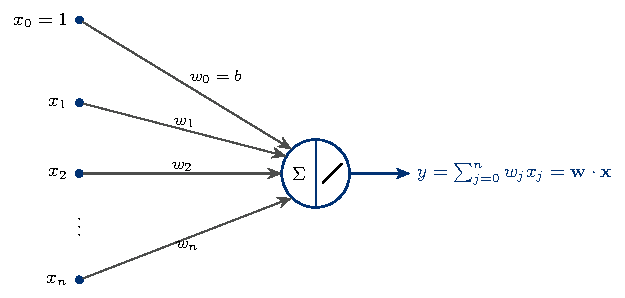
\includegraphics[max width=\linewidth]{Fig22.pdf}
\caption{Neurona lineal con sesgo $b$ y función de activación lineal}
\label{fig22}
\end{figure}

Dado que la función de activación es la identidad, la salida de la neurona está dada por la variable aleatoria unidimencional
$$
Y=\sum_{j=0}^n w_j X_j = \ww\cdot\XX.
$$

La salida deseada de la neurona viene dado por una variable aleatoria unidimensional $Z$. La idea es ajustar el vector de parámetros $\ww$ para que $Y$ aprenda $Z$ y el algoritmo en este caso es el de minimizar la esperanza del cuadrado de la diferencia, por lo que el parámetro óptimo es
$$
\ww^* = \argmin_{\ww} \E[(Z-Y)^2].
$$
Necesitamos encontrar $\ww^*$ y veremos algunas formas de hacerlo, algunas más teóricas y otras más efectivas computacionalmente.

\subsection*{Solución exacta} En este caso $\ww^*$ puede hallarse exactamente. En efecto
\begin{align*}
\E[(Z-Y)^2] &= \E[Z^2 - 2ZY + Y^2] = \E[Z^2 - 2Z\ww\cdot \XX + (\ww\cdot\XX)^2]\\
&= \E[Z^2] - 2\E[Z\XX]\cdot\ww + \E[(\ww\XX^t)(\XX\ww^t)]\\
&= \E[Z^2] - 2\E[Z\XX]\cdot\ww + \ww \E[\XX^t \XX]\ww^t\\
&= \gamma-2\bb\cdot \ww + \ww A\ww^t,
\end{align*}
donde $\gamma=\E[Z^2]$ es el segundo momento de la variable objetivo $Z$, $\bb=\E[Z\XX]$ es el vector que mide la correlación cruzada entre la entrada y la salida, y
$$
A =  \E[\XX^t \XX] = \begin{pmatrix}
\E[X_0 X_0] & \E[X_0 X_1] & \cdots & \E[X_0 X_n]\\
\E[X_1 X_0] & \E[X_1 X_1] & \cdots & \E[X_1 X_n]\\
\vdots & \vdots & \ddots & \vdots\\
\E[X_n X_0] & \E[X_n X_1] & \cdots & \E[X_n X_n]
\end{pmatrix}
$$
es la matriz que describe la autocorrelación de las entradas. En el análisis que haremos vamos a asumir que $A$ es no-degenerada y definida positiva (es decir, las entradas son {\em coherentes}).

Vamos a notar a la función cuadrática por
$$
\xi(\ww) = \gamma-2\bb\cdot\ww + \ww A \ww^t,
$$
su gradiente viene dado entonces por $(\nabla_\ww \xi(\ww))^t = 2A\ww^t - 2\bb^t$ y luego el valor del peso óptimo es la solución de $\nabla_\ww \xi(\ww)=0$ que es la solución del sistema lineal $A\ww^t = \bb^t$. Como la matriz $A$ es no-degenerada, el sistema tiene una solución única dada por $(\ww^*)^t = A^{-1}\bb^t$. Este punto es un mínimo dado que la matriz $A$ es definida positiva. La ecuación $A\ww^t=\bb^t$ dice que $\E[(Z-\ww^*\cdot\XX)X_j]=0$ para $j=0,\dots,n$ (las {\em ecuaciones normales}): el error $Z-Y^*$ es ortogonal en $L^2$ a las entradas, es decir, $Y^*=\ww^*\cdot\XX$ es la proyección ortogonal de $Z$ sobre el subespacio generado por $X_0,\dots,X_n$ (en línea con la Sección~\ref{sec.c3.2}). Notemos además que $A$ es siempre semidefinida positiva, y es definida positiva si y sólo si no hay una combinación lineal no trivial de $X_0,\dots,X_n$ que sea nula casi seguramente.

\subsection*{Método de descenso de gradiente} En general, cuando $n$ es grande, el cálculo de $A^{-1}$ resulta muy costoso y si la matriz está mal condicionada puede traer grandes errores en su cálculo. Es por eso que resulta conveniente usar métodos de aproximación, como el método de descenso, para el cálculo efectivo de $\ww^*$.

Empezamos entonces con un vector de pesos arbitrario $\ww_0\in\R^{n+1}$ y construimos la aproximación $\{\ww_j\}_{j\ge 1}$ recursivamente como
\begin{align*}
\ww_{j+1} &= \ww_j - \eta \nabla_\ww \xi(\ww_j) \\
&= \ww_j - 2\eta (A\ww_j^t - \bb^t)^t\\
&= [(\II_{n+1} - 2\eta A)\ww_j^t + 2\eta\bb^t]^t\\
&=[M\ww_j^t + 2\eta\bb^t]^t,
\end{align*}
donde $\II_{n+1}$ es la matriz identidad de tamaño $(n+1)\times(n+1)$ y $M=\II_{n+1} - 2\eta A$.

\subsection*{Convergencia del método} Veamos para este caso que la iteración converge a la solución buscada. Si iteramos la recursión, obtenemos la siguiente fórmula para $\ww_j$
\begin{align*}
\ww_j^t &= M^j \ww_0^t + (M^{j-1} + M^{j-2} + \cdots + M + \II_{n+1})2\eta\bb^t\\
&= M^j \ww_0^t + (\II_{n+1}-M^j)(\II_{n+1} - M)^{-1}2\eta\bb^t\\
&= M^j \ww_0^t + (\II_{n+1} - M^j) A^{-1}\bb^t.
\end{align*}
Asumamos por un momento que la tasa de aprendizaje $\eta>0$ es tal que 
$$
\lim_{j\to\infty} M^j = \OO_{n+1} \quad \text{(la matriz nula)}.
$$
Entonces, tomando el límite en la fórmula previa obtenemos que
$$
(\ww^*)^t = \lim_{j\to\infty} \ww_j^t = A^{-1}\bb^t
$$

Veamos ahora la suposición de que $M^j\to \OO_{n+1}$. Como $M$ es una matriz simétrica, resulta diagonalizable con autovalores reales y a partir de ahí es fácil ver que la suposición resulta equivalente a ver que los autovalores de $M$, $\{\lambda_i\}_{1\le i\le n+1}$, verifican que $|\lambda_i|<1$

\subsubsection*{Paso 1} Veamos que $\lambda_i<1$.

Observemos que si $\lambda_i$ es un autovalor de $M$, de la definición de $M$ sigue que $\alpha_i = \frac{1-\lambda_i}{2\eta}$ es un autovalor de $A$. Pero como $A$ es definida positiva implica que $\alpha_i>0$ lo que nos da que $\lambda_i<1$.

\subsubsection*{Paso 2} Veamos que si $\eta$ es pequeño, entonces $\lambda_i>-1$.

Notemos por $\{\alpha_i\}_{1\le i\le n+1}$ a los autovalores de $A$. Por el Paso 1, $\lambda_i=1-2\eta\alpha_i$, así que $\lambda_i>-1$ es equivalente a $\eta\alpha_i<1$. Luego, si elegimos la tasa de aprendizaje como
$$
0<\eta<\frac{1}{\alpha_\text{max}},\qquad \alpha_\text{max}=\max_{i}\alpha_i,
$$
obtenemos $|\lambda_i|<1$ para todo $i$. (Esta es exactamente la condición $\eta'<2/\lambda_\text{max}$ del Capítulo~\ref{cap4} para el paso $\eta'=2\eta$ y $\xi$ de Hessiano $2A$.)

\subsection*{Estimación del error} Estimemos ahora el error de la $j-$ésima iteración, $\ve_j = \|\ww_j-\ww^*\|$, usando la fórmula para $\ww_j$, recordando que $(\ww^*)^t=A^{-1}\bb^t$. Tenemos entonces
$$
\ww_j^t - (\ww^*)^t = M^j \ww_0^t + (\II_{n+1} - M^j)(\ww^*)^t - (\ww^*)^t = M^j(\ww_0 - \ww^*)^t.
$$
Luego
$$
\ve_j = \|\ww_j-\ww^*\| = \|M^j(\ww_0 - \ww^*)^t\|\le \|M\|^j \|\ww_0-\ww^*\| = \mu^j d,
$$
donde $\mu=\|M\|$ (la norma como operador) y $d=\|\ww_0-\ww^*\|$.

Ahora, es fácil ver que $\|M\| = \max_{1\le i\le n+1} |\lambda_i|$, pero como $|\lambda_i|<1$ para todo $i$, tenemos que $\mu<1$, por lo que $\mu^j d \to 0$ cuando $j\to\infty$. Más precisamente, $\mu=\max\{|1-2\eta\alpha_\text{min}|,|1-2\eta\alpha_\text{max}|\}$, y la mejor elección es $\eta=1/(\alpha_\text{min}+\alpha_\text{max})$, que da $\mu=\frac{\kappa-1}{\kappa+1}$ con $\kappa=\alpha_\text{max}/\alpha_\text{min}$ el número de condición de $A$: cuanto peor condicionada está $A$, más lenta es la convergencia.

\section{Neurona de entrada continua}\label{sec.5.8}\label{sec.c5.6}

En esta sección introducimos el concepto de {\em neurona de entrada continua}, que es una neurona con una cantidad no numerable de pesos. Este concepto será usado más adelante en la sección \ref{sec.7.3} para la construcción de redes neuronales continuas. 

Recomiendo consultar también el capítulo 10 de \cite{Calin} donde se estudia el aprendizaje en el contexto de neuronas de entrada continua.

Una neurona de entrada continua tiene como entrada $x\in [a, b]$. El peso asociado al valor $x$ viene dado por $w(dx)$, donde $w$ es una medida sobre el intervalo $[a, b]$. La primera mitad de la unidad de cómputo integra las entradas con respecto a la medida $w$. La función de salida en este caso toma la forma
\begin{equation}\label{5.8.7}
y=\sigma\left(\int_a^b x\, dw(x)\right).
\end{equation}
En particular esto se aplica a la situación en donde la entrada es una variable aleatoria que toma valores en el intervalo $[a, b]$. Si $w$ representa la medida de distribución de $X$, entonces la salida de la neurona depende de su esperanza, $y=\sigma(\E[X])$.

Dependiendo del tipo particular de medida de peso que se utilice, la fórmula \eqref{5.8.7} provee de una representación general para la salida de una neurona tanto si tiene un número finito de entradas, como discutimos previamente, un número infinito numerable o un número no numerable de entradas. 

Veamos algunos ejemplos.
\begin{ejem}[Neurona con una medida de Dirac]
Sea $x_0\in [0,1]$ fijo y consideremos la medida de Dirac $\delta_{x_0}$ definida por
$$
\delta_{x_0}(A) = \begin{cases}
1, & \text{si } x_0\in A\\
0, & \text{si } x_0\not\in A,
\end{cases}
$$
para cualquier conjunto medible $A$. Esto corresponde al caso en que la variable aleatoria $X$ toma sólo el valor $x_0$. La función de salida en este caso es una constante
$$
y=\sigma\left(\int_a^b x\, d\delta_{x_0}(x)\right) = \sigma(x_0).
$$
Dado que no hay parámetros que ajustar, no hay nada que aprender.
\end{ejem}

\begin{ejem}[Neurona con una medida discreta]
Sea $E=\{x_1,\dots,x_n\}$ un conjunto finito de puntos del intervalo $[0,1]$ y consideremos la medida discreta
$$
\mu(A) = \sum_{x_j\in E} w_j \delta_{x_j}(A),
$$
donde el número positivo $w_j$ es la masa del punto $x_j$. La función de salida está dada por
$$
y=\sigma\left(\int_a^b x\, d\mu(x)\right) = \sigma\left(\sum_{j=1}^n w_j x_j\right),
$$
que corresponde al modelo de neurona clásico. El algoritmo de aprendizaje en este caso ajusta los pesos $w_j$ para minimizar la función de error, por ejemplo,
$$
F(w) = \frac12 \left(\sigma\left(\sum_{j=1}^n w_j x_j\right) - z\right)^2,
$$
donde $z$ es el valor deseado de la neurona dada la observación $\xx = (x_1,\dots, x_n)$.
\end{ejem}

\begin{ejem}[Neurona con medida continua]
Sea $\mu$ una medida absolutamente continua con respecto a la medida de Lebesgue. Es decir $d\mu(x) = p(x)dx$ para una función no negativa y medible $p$ en el intervalo $[0,1]$. Luego, la función de salida de la neurona está dada por
$$
y=\sigma\left(\int_0^1 x\, d\mu(x)\right)=\sigma\left(\int_0^1 x p(x)\, dx\right),
$$
que depende de la función de peso $p(x)$. El algoritmo debe entonces optimizar la neurona eligiendo la función $p(x)$ que minimice el {\em funcional de error}
$$
F(p) = \frac12\left(\sigma\left(\int_0^1 x p(x)\, dx\right) - z\right)^2
$$
Si $\mu$ es una {\em medida de probabilidad}, entonces $p(x)$ es una densidad de probabilidad lo que implica que $\int_0^1 p(x)\, dx =1$. Luego, si suponemos que $p(x)$ minimiza la función de error, debe verificar que 
$$
F(p)\le F(q)
$$
para toda densidad de probabilidad $q(x)$. Para encontrar esta densidad óptima se usa el {\em cálculo de variaciones}. Asumamos que $p$ es óptima y, para simplificar, que $p\ge c>0$ en $[0,1]$. Sea $\varphi$ acotada con $\int_0^1\varphi(x)\, dx = 0$. Entonces, para $|t|$ chico, $p_t(x) = p(x) + t\varphi(x)$ es no negativa y verifica $\int_0^1 p_t(x)\, dx=1$, de modo que es una densidad y, por ende,
$$
F(p) \le F(p_t),\quad \text{para todo } |t| \text{ suficientemente chico.}
$$
Luego, si $j(t) = F(p_t)$ tenemos que $j(t)$ alcanza su mínimo en $t=0$ por lo que se debe tener $j'(0)=0$. Notemos por $m(p)=\int_0^1xp(x)\,dx$. Entonces
\begin{align*}
j'(0) &= \bigl(\sigma(m(p)) - z\bigr)\,\sigma'(m(p))\,\frac{d}{dt}\Big|_{t=0}\int_0^1 x p_t(x)\, dx\\
&=\bigl(\sigma(m(p)) - z\bigr)\,\sigma'(m(p))\int_0^1 x \varphi(x)\, dx.
\end{align*}
Elijamos $\varphi(x)=x-\tfrac12$, que cumple $\int_0^1\varphi\,dx=0$ y $\int_0^1x\varphi(x)\,dx=\tfrac13-\tfrac14=\tfrac1{12}\ne0$. Como $\sigma'>0$ (por ejemplo, para la función logística), $j'(0)=0$ si y sólo si
$$
\sigma\left(\int_0^1 x p(x)\, dx\right) = z,
$$
lo que nos da una condición necesaria para encontrar al mínimo del funcional. Notemos que $F$ depende de $p$ solo a través de $m(p)\in(0,1)$; en particular, la condición solo puede cumplirse si $z\in(\sigma(0),\sigma(1))\approx(0{,}5;\,0{,}731)$ para la logística. Si $z$ está fuera de ese rango, el ínfimo de $F$ no se alcanza con una densidad.
\end{ejem}

\section{Resumen}\label{sec.c5.7}
En este capítulo se presentaron distintos tipos de neuronas. Obviamente existen más tipos, pero hemos elegido presentar las más clásicas: Perceptrón, sigmoide y lineal. Todas las neuronas se caracterizan por una entrada, un sistema de pesos, un sesgo, una función de activación y una salida.

El perceptrón es un modelo de neurona con una función escalón como función de activación. La neurona dispara si la señal de entrada supera un cierto umbral. Su salida tiene una discontinuidad de salto. Un perceptrón puede ser usado como un clasificador binario para clasificar dos clústeres que son linealmente separables. Puede ser también usado para aprender funciones Booleanas como AND y OR, pero no puede aprender la función XOR.

La neurona sigmoideal tiene una función de activación sigmoideal. Su salida es continua y puede saturar si la señal es o muy grande o muy pequeña. La neurona sigmoideal puede aprender usando regresión logística, que es equivalente al hecho de que los pesos vengan dados por el método de máxima verosimilitud. Presentamos algunas aplicaciones de esta neurona como clasificación binaria y predicción de probabilidades.

Las neuronas lineales tienen entradas a variables aleatorias y la función de activación es lineal. Sus pesos óptimos pueden ser obtenidos de manera exacta aunque en aplicaciones prácticas es mejor y más simple entrenar a la neurona con un método de descenso de gradiente.

\section{Ejercicios}\label{sec.c5.8}

\begin{ejer}\label{ej.neg}
Recordemos que $\neg x$ es la negación de la variable Booleana $x$.
\begin{itemize}
\item[(a)] Mostrar que un perceptrón puede aprender la función Booleana $y=x_1\wedge \neg x_2$, con $x_1, x_2\in \{0,1\}$

\item[(b)] Misma pregunta que en (a) para la función Booleana $y=x_1\vee \neg x_2$.

\item[(c)] Mostrar que un perceptrón con una entrada Booleana $x$ puede aprender la negación $y=\neg x$. ¿Qué sucede si queremos usar una neurona lineal?

\item[(d)] Mostrar que un perceptrón con tres entradas Booleanas $x_1, x_2, x_3$ puede aprender $x_1\wedge x_2\wedge x_3$. ¿Qué sucede con $x_1\vee x_2\vee x_3$?
\end{itemize}
\end{ejer}

\begin{ejer}
Mostrar que dos conjuntos finitos y linealmente separables $A$ y $B$ pueden ser separados por un perceptrón con pesos racionales.
\end{ejer}

\begin{ejer}
\begin{itemize}
\item[(a)] Asumamos que las entradas de una neurona lineal son independientes y normalmente distribuidas, $X_i\sim N(0,\sigma_i^2)$, $i=1,\dots,n$. Hallar los pesos óptimos $\ww^*$.

\item[(b)] Una variable aleatoria unidimensional con media cero, $Z$, es aprendida por una neurona lineal con entrada $X$. Asumamos que la entrada $\XX$ y el objetivo $Z$ son independientes. Escribir la función de costo y hallar los parámetros óptimos $\ww^*$. Interpretar el resultado.
\end{itemize}
\end{ejer}

\begin{ejer}
Mostrar la equivalencia entre el algoritmo de regresión lineal y el de aprendizaje de una neurona lineal.
\end{ejer}

\begin{ejer}\label{ej.perceptron}
Considerar $n$ puntos, $P_1,\dots, P_n$ incluidos en media circunferencia y notemos por $\xx_1,\dots,\xx_n$ sus coordenadas. Un perceptrón puede aprender la mencionada media circunferencia usando el siguiente algoritmo:
\begin{enumerate}
\item Empezamos por una media circunferencia arbitraria determinada por su diámetro y un vector unitario $\ww_0$. Entonces seleccionamos un punto incorrectamente clasificado $P_{i_0}$, i.e. un punto tal que $\ww_0\cdot\xx_{i_0}<0$. Ver Figura \ref{fig23}.

\item Rotemos el diámetro de manera tal que la nueva normal es $\ww_1 = \ww_0 + \xx_{i_0}$. Mostrar que $\ww_1\cdot\xx_{i_0}=\ww_0\cdot\xx_{i_0}+\|\xx_{i_0}\|^2>\ww_0\cdot\xx_{i_0}$: el valor aumenta, de modo que $P_{i_0}$ está más cerca de quedar bien clasificado (puede ser necesario repetir el paso).

\item Repitiendo las dos etapas previas, construimos inductivamente una sucesión de vectores $\{\ww_m\}_{m\ge 1}$ tal que $\ww_{m+1} = \ww_m + \xx_{i_m}$, donde $P_{i_m}$ es un punto mal clasificado en la etapa $m$. Mostrar que este proceso termina en un número finito de pasos si los puntos admiten un margen, es decir, si existe $\ww^*$ unitario y $\gamma>0$ con $\ww^*\cdot\xx_i\ge\gamma$ para todo $i$ (esto ocurre si los puntos están en un semiplano abierto, pero no si hay dos puntos antípodas sobre el borde). {\em Sugerencia:} partiendo de $\ww_0=0$, probar que $\ww_m\cdot\ww^*\ge m\gamma$ y que $\|\ww_m\|^2\le mR^2$, con $R=\max_i\|\xx_i\|$, y concluir que $m\le(R/\gamma)^2$. Este es el {\em teorema de convergencia del perceptrón} de Novikoff.
\end{enumerate}
\end{ejer}

\begin{figure}[htbp]
\centering
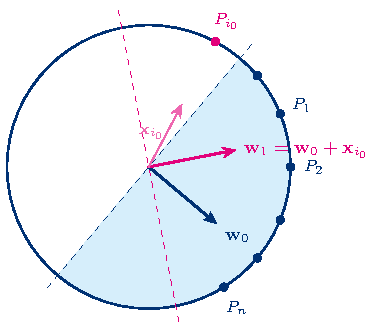
\includegraphics[max width=\linewidth]{Fig23.pdf}
\caption{Figura para el Ejercicio \ref{ej.perceptron}}
\label{fig23}
\end{figure}

\begin{ejer}
Modificar el algoritmo del ejercicio anterior para el caso en que los puntos $P_1,\dots, P_n$ están incluidos en un semi espacio. 
\end{ejer}

\begin{ejer}
Notemos por $\I_A(x)$ a la función caraterística (o indicadora) del conjunto $A$, es decir $\I_A(x) = 1$ si $x\in A$ y $\I_A(x)=0$ si $x\not\in A$.
\begin{itemize}
\item[(a)] Mostrar que la función
$$
\varphi(x_1, x_2) = \I_{\{x_2>x_1+0.5\}}(x_1, x_2) + \I_{\{x_2<x_1-0.5\}}(x_1, x_2)
$$
implementa XOR.

\item[(b)] Mostrar que XOR puede ser implementada por una combinación lineal de dos perceptrones.
\end{itemize}
\end{ejer}

%%%%%%%%%%%%%%%%%%%%%%%%%%%%%%%%%%%%%%%%
%% CAPITULO 6 %%%%%%%%%%%%%%%%%%%%%%%%%%%%%%%
%%%%%%%%%%%%%%%%%%%%%%%%%%%%%%%%%%%%%%%%

\chapter{Redes neuronales}\label{cap6}

Hasta el momento hemos discutido el caso de una única neurona. En esta sección consideraremos varias capas de neuronas cuyas salidas alimentan otras capas de neuronas formando así {\em redes neuronales}. Una capa de neuronas es un paso de procesamiento en una red neuronal y puede haber de distintos tipos, dependiendo de los pesos y de las funciones de activación usada en sus neuronas. La parte principal de esta capítulo trata sobre el entrenamiento de redes neuronales usando el {\em algoritmo de retropropagación} (backpropagation algorithm en inglés).

Dado que el estudio de redes neuronales se basa fuertemente en notación, empezamos con un ejemplo de calentamiento.

Las neuronas se organizan en capas. Se trabaja primero un ejemplo completo (Sección~\ref{sec.c6.1}), donde aparece el cálculo del gradiente por retropropagación; luego se lo hace en general (Sección~\ref{sec.c6.2}), y se discute cómo inicializar los pesos (Sección~\ref{sec.c6.3}). Corresponde al Capítulo~6 de~\cite{Calin}.

\section{Un ejemplo de red neuronal}\label{sec.c6.1}

Consideremos dos neuronas que tienen idénticas entradas $x_1, x_2$ y diferentes salidas $y_1$ e $y_2$ respectivamente. Las salidas se usan para alimentar una tercera neurona con salida $y$. Ver figura \ref{fig24}. Asumimos que la función de activación de todas las neuronas es la misma y la notamos por $\varphi$. Cada neurona tiene un sesgo que es considerado como un peso de una ``falsa'' entrada igual a $-1$. Ahora ensamblamos estas neuronas juntas como una red neuronal equivalente, como se ve en la Figura \ref{fig25}. Esto forma una capa de dos neuronas en el medio que se la llama la {\em capa escondida}.

\begin{figure}[htbp]
\centering
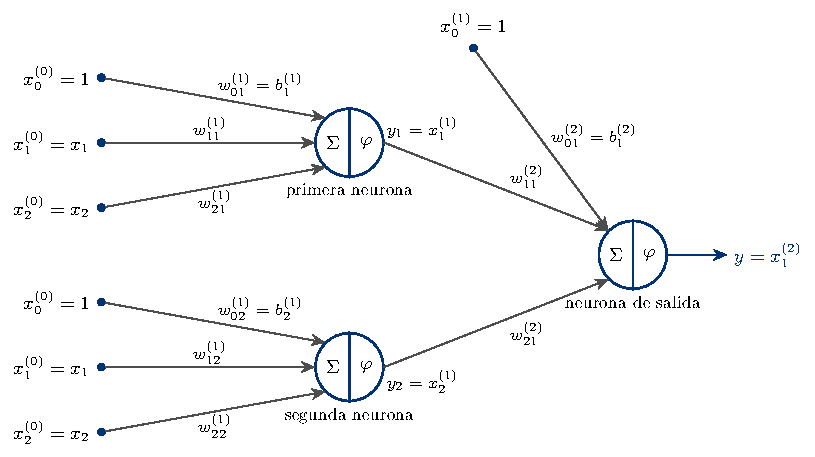
\includegraphics[max width=\linewidth]{Fig24.pdf}
\caption{Dos neuronas con idénticas entradas $x_1, x_2$, y salidas $y_1, y_2$ que alimentan una tercera neurona con salida $y$.}
\label{fig24}
\end{figure}

Las sinapsis entre las neuronas están representadas por ejes y cada uno de esos es asociado con un peso, notado por $w_{ij}^{(\ell)}$. Los índices tienen el siguiente significado: El superíndice, $(\ell)$, representa el índice de la capa en la que entra la sinapsis. El índice $\ell=1$ es usado para los pesos que alimentan la capa escondida y el índice $\ell=2$ es usado para los pesos que entran en la capa de salida, que consiste en la última neurona. El índice inferior $i$ indica la neurona de entrada. El índice $i=0$ es siempre usado para el sesgo, mientras que $i=1, 2$ representa el índice de la entrada. El segundo índice, $j$, corresponde a la neurona de salida, i.e., el índice de la neurona a la que apunta la sinapsis. 

\begin{figure}[htbp]
\centering
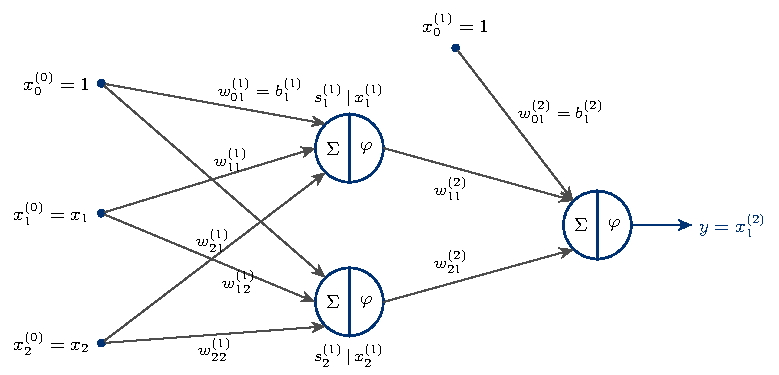
\includegraphics[max width=\linewidth]{Fig25.pdf}
\caption{Red neuronal con una capa escondida, teniendo dos entradas $x_1, x_2$ y dos neuronas en la capa escondida.}
\label{fig25}
\end{figure}

Las entradas forman la {\em primera capa} de la red. Estos se notan con un superíndice igual a 0: $x_0^{(0)}=1$, $x_1^{(0)}$ y $x_2^{(0)}$. Notemos que los sesgos de las neuronas en la capa escondida son notados por $b_1^{(1)} = w_{01}^{(1)}$ y $b_2^{(1)} = w_{02}^{(1)}$, mientras que el sesgo de la neurona en la capa de salida es $b_1^{(2)} = w_{01}^{(2)}$.

La primera neurona de la capa escondida toma la información de la capa de entrada en la señal
$$
s_1^{(1)} = w_{01}^{(1)}  x_0^{(0)} + w_{11}^{(1)}  x_1^{(0)} + w_{21}^{(1)}  x_2^{(0)} = \sum_{i=1}^2 w_{i1}^{(1)}  x_i^{(0)} + b_1^{(1)}.
$$
Luego, se aplica la función de activación $\varphi$ a la señal para obtener la salida
$$
y_1 = x_1^{(1)} = \varphi(s_1^{(1)}) = \varphi\left(\sum_{i=1}^2 w_{i1}^{(1)}  x_i^{(0)} + b_1^{(1)}\right).
$$

De manera análoga, la segunda neurona de la capa escondida toma la información en la señal
$$
s_2^{(1)} = w_{02}^{(1)}  x_0^{(0)} + w_{12}^{(1)}  x_1^{(0)} + w_{22}^{(1)}  x_2^{(0)} = \sum_{i=1}^2 w_{i2}^{(1)}  x_i^{(0)} + b_2^{(1)},
$$
y luego le aplica la función de activación $\varphi$ para obtener la salida
$$
y_2 = x_2^{(1)} = \varphi(s_2^{(1)}) = \varphi\left(\sum_{i=1}^2 w_{i2}^{(1)}  x_i^{(0)} + b_2^{(1)}\right).
$$

Estas relaciones pueden ser manipuladas de manera más simple si son escritas en forma matricial. Las señales en la capa escondida se pueden escribir como
$$
\begin{pmatrix}
s_1^{(1)} \\
s_2^{(1)}
\end{pmatrix} =
\begin{pmatrix}
w_{11}^{(1)} & w_{21}^{(1)}\\
w_{12}^{(1)} & w_{22}^{(1)}
\end{pmatrix}
\begin{pmatrix}
x_1^{(0)} \\
x_2^{(0)}
\end{pmatrix} - 
\begin{pmatrix}
b_1^{(1)} \\
b_2^{(1)}
\end{pmatrix},
$$
o en forma condensada como
$$
\sbf^{(1)} = W^{(1)^t} \xx^{(0)} + \bb^{(1)},
$$
donde $\sbf^{(1)}$ representa el vector de señales, $W^{(1)}$ es la matriz de pesos, $\xx^{(0)}$ es el vector de entrada y $\bb^{(1)}$ es el vector de sesgos para las neuronas en la capa escondida. Observemos que se toma la transpuesta en $W^{(1)}$ por como hemos elegido la numeración de los coeficientes y en esta ocasión tomamos los vectores  $\sbf^{(1)}$, $\xx^{(0)}$ y $\bb^{(1)}$ como vectores columna.

La salida de la capa escondida es el vector
$$
\xx^{(1)} = \begin{pmatrix}
y_1 \\
y_2
\end{pmatrix} = \begin{pmatrix}
x_1^{(1)} \\
x_2^{(1)}
\end{pmatrix} = \begin{pmatrix}
\varphi(s_1^{(1)}) \\
\varphi(s_2^{(1)})
\end{pmatrix} = \varphi(\sbf^{(1)}),
$$
donde adoptamos la convención de que aplicar la función $\varphi$ a un vector da como resultado un nuevo vector que se calcular aplicando $\varphi$ a cada componente.

Estas dos últimas fórmulas implican la relación
$$
\xx^{(1)} = \varphi(W^{(1)^t} \xx^{(0)} + \bb^{(1)}),
$$
que nos da el vector de salida de la capa escondida como función de las entradas. La multiplicación de $\xx^{(0)}$ por la matriz $W^{(1)^t}$ es una transformación lineal y sumar el vector de sesgos $\bb^{(1)}$ lo convierte en una transformación afín. La función de activación $\varphi$ es la que agrega la no linealidad a la salida.

La neurona de la última capa convierte esta última información en la señal
$$
s^{(2)} = s_1^{(2)} = w_{01}^{(2)}  x_0^{(1)} + w_{11}^{(2)}  x_1^{(1)} + w_{21}^{(2)}  x_2^{(1)} = \sum_{i=1}^2 w_{i1}^{(2)}  x_i^{(1)} + b_1^{(2)}.
$$
En la forma matricial, esto se escribe como
$$
\sbf^{(2)} = W^{(2)^t} \xx^{(1)} + \bb^{(2)},
$$
donde ahora la matriz de coeficientes y el vector de entrada vienen dados por
$$
W^{(2)} = \begin{pmatrix}w_{11}^{(2)} \\ w_{21}^{(2)}\end{pmatrix}\qquad \text{y}\qquad \xx^{(1)} = \begin{pmatrix} x_1^{(1)}\\ x_2^{(1)}\end{pmatrix}.
$$
En este caso, la señal que sale de la última neurona $\sbf^{(2)} = \sbf_1^{(2)}$ es una matriz unidimensional. El subíndice $1$ indica que hay sólo una única neurona en la capa de salida. La salida de la red se obtiene aplicando la función de activación a la señal $\sbf^{(2)}$ de la forma
$$
y = \xx_1^{(2)} = \varphi(\sbf^{(2)}) = \varphi(W^{(2)^t} \xx^{(1)} + \bb^{(2)}).  
$$
Notamos a la salida $y$ para ser consistente con los capítulos previos y también con $\xx_1^{(2)}$ en donde el superíndice $(2)$ indica que es la salida de la segunda capa (en realidad la tercera si contamos la capa de datos de entrada) y el subíndice 1 significa que es la salida de la primera (y única) neurona de esta capa.

Si usamos la fórmula para $\xx^{(1)}$ que obtuvimos, podemos expresar la salida final en términos de las entradas originales como
\begin{equation}\label{formula.y}
y =  \varphi(W^{(2)^t}  \varphi(W^{(1)^t} \xx^{(0)} + \bb^{(1)})   + \bb^{(2)}).  
\end{equation}
Notemos que las transformaciones afines que consisten en multiplicar por las matrices de pesos y sumar los vectores de sesgo, se alternan con la transformación no lineal que es inducida por la función de activación $\varphi$. Si se considera el mapa $f_{w, b}\colon \R^2\to\R$ dado por
$$
f_{w, b}(\xx) =  \varphi(W^{(2)^t}  \varphi(W^{(1)^t} \xx + \bb^{(1)})   + \bb^{(2)}),
$$
lo llamamos el {\em mapa de entrada-salida} de la red neuronal.

\begin{obs}
Observemos que si las neuronas de la red son lineales, i.e. la función de activación es la identidad $\varphi(x)=x$, entonces la salida es
$$
y= (W^{(1)}W^{(2)})^t \xx^{(0)} + W^{(2)^t} \bb^{(1)}+ \bb^{(2)} = W^t\xx^{(0)} + \bb,
$$
donde $W=W^{(1)}W^{(2)}$ y $\bb = W^{(2)^t} \bb^{(1)}+\bb^{(2)}$. Luego toda la red neuronal resulta equivalente a una única neurona. Es decir que el estudio de redes neuronales lineales se reduce al estudio de una única neurona lineal.
\end{obs}

\begin{obs}\label{obsXOR}
Asumamos ahora que la red neuronal de la sección está compuesta por todos perceptrones con función de activación $\varphi(x) = H(x)$. La salida de la red en este caso es dada por
$$
y = H\left(w_1^{(2)} H(x_1 w_{11}^{(1)} + x_2 w_{21}^{(1)} + b_1^{(1)}) + w_2^{(2)} H(x_1 w_{12}^{(1)} + x_2 w_{22}^{(1)} + b_2^{(1)}) + b^{(2)}\right).
$$
Notemos que esta red puede aprender exactamente la función Booleana XOR. En efecto, esto lo logramos eligiendo los pesos de la forma
$$
y=f(x_1, x_2) = H(H(x_1+x_2 - 0.5) - H(x_1+x_2 - 1.5) - 0.5).
$$
Se puede verificar fácilmente que $f(0,0)=f(1,1)=0$ y $f(1,0)=f(0,1)=1$. 

Que tres perceptrones alcanzan se puede explicar de la siguiente manera. En el Ejercicio \ref{ej.neg} vimos que las funciones $y_1 = x_1\wedge \neg x_2$ e $y_2 = \neg x_1\wedge x_2$ pueden ser aprendidas por un perceptrón cada una. Se necesita un perceptrón más para aprender la función $y_1\vee y_2$, que es la función XOR, $(x_1\wedge \neg x_2)\vee (\neg x_1\wedge x_2)$. Que con dos no alcanza se ve así: si hubiera un solo perceptrón oculto, la salida sería función de $H(\ww\cdot\xx+ b_1)\in\{0,1\}$, y por lo tanto sería constante, igual a esa salida, o igual a su negación (que también es un perceptrón), lo que contradice que XOR no es implementable por un solo perceptrón (Capítulo~\ref{cap5}). Notemos que aquí $H(0)=1$, como en el Capítulo~\ref{cap2}.
\end{obs}

\subsection{Variación total y regularización}

El rendimiento de generalización de una red neuronal depende de la sensibilidad de la salida con respecto a su entrada. Asumamos que tenemos dos redes que han sido entrenadas con los mismos datos: la red que se muestra en la figura \ref{fig26} {\bf a}, que sobreajusta a los datos, y la que se muestra en la figura \ref{fig26} {\bf b}, que generaliza bien. La diferencia geométrica entre estos modelos consiste en el hecho de que en el primer caso la variación total de la salida es mayor a la de la segunda. La variación total está relacionada a la sensibilidad de la salida por la fórmula. Si $y=f(\xx^{(0)})$ denota el mapa de entrada-salida de la red, la variación total representa la acumulación total de las variaciones locales
$$
V(f) = \int \|\nabla f(\xx)\|\,d\xx,
$$
donde la integral se calcula sobre el espacio de entrada (o sobre una región acotada de él). Luego, la variación total $V(f)$ juega un rol importante al evaluar la performance de evaluación de la red y es el motivo por el que es necesario contar con una fórmula para el diferncial $dy = df(\xx)$ y lo calcularemos en lo que sigue.

\begin{figure}[htbp]
\centering
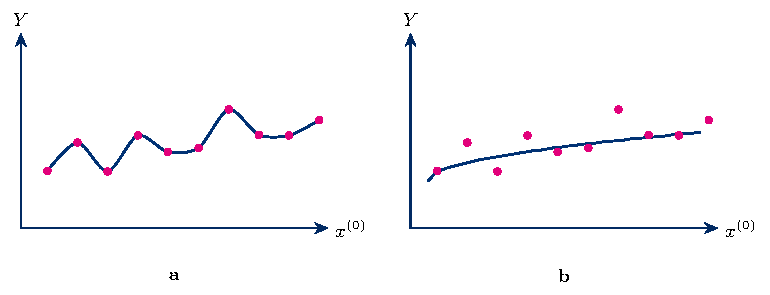
\includegraphics[max width=\linewidth]{Fig26.pdf}
\caption{{\bf a.} El modelo sobreajusta los datos de entrada. {\bf b.} El modelo generaliza bien.}
\label{fig26}
\end{figure}

La fórmula \eqref{formula.y} nos da la salida en función de la entrada. Asumiendo que los pesos y sesgos se mantienen fijos, los cambios en la salida $y$ cuando se producen pequeños cambios en las entradas $\xx^{(0)}$ se calculan aplicando la regla de la cadena:
\begin{align*}
dy &= \frac{dy}{d\sbf^{(2)}} d\sbf^{(2)} =  \frac{dy}{d\sbf^{(2)}} \frac{d\sbf^{(2)}}{d\xx^{(1)}} d\xx^{(1)}\\
&= \frac{dy}{d\sbf^{(2)}} \frac{d\sbf^{(2)}}{d\xx^{(1)}} \frac{d\xx^{(1)}}{d\sbf^{(1)}} d\sbf^{(1)} \\
&= \frac{dy}{d\sbf^{(2)}} \frac{d\sbf^{(2)}}{d\xx^{(1)}} \frac{d\xx^{(1)}}{d\sbf^{(1)}} \frac{d\sbf^{(1)}}{d\xx^{(0)}} d\xx^{(0)}.
\end{align*}
Usando que 
\begin{align*}
&\frac{dy}{d\sbf^{(2)}} = \varphi'(\sbf^{(2)}), \qquad \frac{d\xx^{(1)}}{d\sbf^{(1)}} = D^{(1)}:=\operatorname{diag}\bigl(\varphi'(s_1^{(1)}),\varphi'(s_2^{(1)})\bigr),\\
&\frac{d\sbf^{(2)}}{d\xx^{(1)}}  = W^{(2)^t}, \qquad \frac{d\sbf^{(1)}}{d\xx^{(0)}}  = W^{(1)^t},
\end{align*}
obtenemos
\begin{equation}\label{dy}
dy = \varphi'(\sbf^{(2)}) W^{(2)^t} D^{(1)} W^{(1)^t} d\xx^{(0)}.
\end{equation}

A partir de la fórmula \eqref{dy} vemos que existe una relación entre el valor de la variación $V(f)$ y los pesos $W^{(\ell)}$, $\ell=1, 2$. Más precisamente, como $|Au|\le\|A\|_{op}|u|$ para la norma operador, resulta $|dy|\le \bigl(\sup|\varphi'|\bigr)^2\,\|W^{(2)}\|_{op}\|W^{(1)}\|_{op}\,|d\xx^{(0)}|$, de donde $f$ es Lipschitz con esa constante y $V(f)\le \mathrm{Lip}(f)\,|\Omega|$ sobre un dominio acotado $\Omega$. Luego, si requerimos que estos pesos sean pequeños en norma operador, esto hará disminuir $V(f)$. Heurísticamente, esto mejora la performance de generalización (es una de las motivaciones de la regularización de la Sección~\ref{sec.c3.3}). Para la logística, $\sigma'\le\frac14$ (Ejercicio~2.1), de modo que cada capa aporta un factor $\le\frac14$ a la cota: en redes profundas esto produce el problema del {\em gradiente evanescente}.

En el caso cuando la función de activación es la función logística $\varphi=\sigma$, usando propiedades de la logística, la fórmula \eqref{dy} se puede escribir en la forma
$$
dy = \sigma(\sbf^{(2)})(1-\sigma(\sbf^{(2)})) W^{(2)^t}\, \operatorname{diag}\bigl(\sigma(\sbf^{(1)})(1-\sigma(\sbf^{(1)}))\bigr)\, W^{(1)^t} d\xx^{(0)},
$$
donde el producto $\sigma(\sbf^{(1)})(1-\sigma(\sbf^{(1)}))$ se entiende componente a componente.
Esta fórmula será útil en la resolución de algunos de los ejercicios.

\subsection{Retropropagación}

Consideremos una función de costo $C(w, b)$ que mide la proximidad entre la salida de la red $y=f_{w, b}(\xx)$ y el objetivo $z$.  Asumamos que la función de costo es una función suave de los pesos y sesgos. Su gradiente está dado por
$$
\nabla C = (\nabla_w C, \nabla_b C).
$$
Para la red que vimos en el ejemplo, este vector tiene dimensión nueve, dependiendo de seis pesos y tres sesgos. Vamos a realizar el cálculo de este gradiente hacia atrás, desde los últimos pesos y sesgos hacia los primeros por un procedimiento que se llama {\em retropropagación}.

Empezamos calculando las derivadas parciales de la función de costo con respecto a los pesos que tienen superíndice $\ell=2$. Vamos también a usar que la función de costo $C$ depende de $y$ que a su vez depende de $w_{ij}^{(2)}$ a través de $\sbf_1^{(2)}$ como $y=\varphi(\sbf_1^{(2)})$. Aplicando la regla de la cadena obtenemos
\begin{align*}
\frac{\partial C}{\partial b_1^{(2)}} = \frac{\partial C}{\partial w_{01}^{(2)}} &= \frac{\partial C}{\partial s_1^{(2)}} \frac{\partial s_1^{(2)}}{\partial w_{01}^{(2)}} = \delta_1^{(2)} x_0^{(1)} = \delta_1^{(2)}\\
\frac{\partial C}{\partial w_{11}^{(2)}} &= \frac{\partial C}{\partial s_1^{(2)}} \frac{\partial s_1^{(2)}}{\partial w_{11}^{(2)}} = \delta_1^{(2)} x_1^{(1)}\\
\frac{\partial C}{\partial w_{21}^{(2)}} &= \frac{\partial C}{\partial s_1^{(2)}} \frac{\partial s_1^{(2)}}{\partial w_{21}^{(2)}} = \delta_1^{(2)} x_2^{(1)},
\end{align*}
donde usamos el hecho de que $s^{(2)} = w_{01}^{(2)} x_0^{(1)} + w_{11}^{(2)} x_1^{(1)} + w_{21}^{(2)} x_2^{(1)}$, $x_0^{(1)}=1$ y usamos la notación $\delta_1^{(2)} = \frac{\partial C}{\partial s_1^{(2)}}$.

Ahora calculamos las derivadas parciales con respecto a los pesos y sesgos con superíndice $\ell=1$. El costo $C$ depende de $y$, que a su vez depende de $w_{ij}^{(1)}$ a través de $s_j^{(1)}$, $j=1,2$, dado que $y=\varphi(W^{(2)^t}\varphi(\sbf^{(1)}) + \bb^{(2)})$ por \eqref{formula.y}. Para $j=1$ la regla de la cadena nos da
\begin{align*}
\frac{\partial C}{\partial b_1^{(1)}} = \frac{\partial C}{\partial w_{01}^{(1)}} &= \frac{\partial C}{\partial s_1^{(1)}} \frac{\partial s_1^{(1)}}{\partial w_{01}^{(1)}} = \delta_1^{(1)} x_0^{(0)} = \delta_1^{(1)}\\
\frac{\partial C}{\partial w_{11}^{(1)}} &= \frac{\partial C}{\partial s_1^{(1)}} \frac{\partial s_1^{(1)}}{\partial w_{11}^{(1)}} = \delta_1^{(1)} x_1^{(0)}\\
\frac{\partial C}{\partial w_{21}^{(1)}} &= \frac{\partial C}{\partial s_1^{(1)}} \frac{\partial s_1^{(1)}}{\partial w_{21}^{(1)}} = \delta_1^{(1)} x_2^{(0)},
\end{align*}
donde ahora $\delta_1^{(1)} = \frac{\partial C}{\partial s_1^{(1)}}$. Para $j=2$ nos queda
\begin{align*}
\frac{\partial C}{\partial b_2^{(1)}} = \frac{\partial C}{\partial w_{02}^{(1)}} &= \frac{\partial C}{\partial s_2^{(1)}} \frac{\partial s_2^{(1)}}{\partial w_{02}^{(1)}} = \delta_2^{(1)} x_0^{(0)} = \delta_2^{(1)}\\
\frac{\partial C}{\partial w_{12}^{(1)}} &= \frac{\partial C}{\partial s_2^{(1)}} \frac{\partial s_2^{(1)}}{\partial w_{12}^{(1)}} = \delta_2^{(1)} x_1^{(0)}\\
\frac{\partial C}{\partial w_{22}^{(1)}} &= \frac{\partial C}{\partial s_2^{(1)}} \frac{\partial s_2^{(1)}}{\partial w_{22}^{(1)}} = \delta_2^{(1)} x_2^{(0)},
\end{align*}
donde $\delta_2^{(1)} = \frac{\partial C}{\partial s_2^{(1)}}$.

Resumiendo estos cálculos, tenemos
\begin{align}
\frac{\partial C}{\partial b_j^{(\ell)}} &= \delta_j^{(\ell)}\\
\frac{\partial C}{\partial w_{ij}^{(\ell)}} &= \delta_j^{(\ell)} x_i^{(\ell-1)}.
\end{align}
Es decir que el gradiente de la función de costo, $\nabla C$, lo conocemos si podemos calcular los valores de $\delta_j^{(\ell)}$. Veamos que las deltas de la capa oculta, $\delta_j^{(1)}$ $(j=1,2)$, dependen del delta de la capa final $\delta_1^{(2)}$. Usando que $s_1^{(1)}$ afecta a la función de costo $C$ sólo a través de $s_1^{(2)}$, la regla de la cadena nos da
\begin{equation}\label{delta1}
\delta_1^{(1)} = \frac{\partial C}{\partial s_1^{(1)}} =  \frac{\partial C}{\partial s_1^{(2)}} \frac{\partial s_1^{(2)}}{\partial s_1^{(1)}} = \delta_1^{(2)}\frac{\partial s_1^{(2)}}{\partial s_1^{(1)}}.
\end{equation}

Ahora, la señal $s_1^{(2)}$ se escribe como
$$
s_1^{(2)} = w_{01}^{(2)} + w_{11}^{(2)}\varphi(s_1^{(1)}) + w_{21}^{(2)}\varphi(s_2^{(1)}),
$$
entonces sigue que
$$
\frac{\partial s_1^{(2)}}{\partial s_1^{(1)}} =  w_{11}^{(2)}\varphi'(s_1^{(1)}).
$$
Reemplazando en \eqref{delta1}, obtenemos
$$
\delta_1^{(1)} = \delta_1^{(2)} w_{11}^{(2)}\varphi'(s_1^{(1)}).
$$
De manera análoga,
$$
\delta_2^{(1)} = \delta_1^{(2)} w_{21}^{(2)}\varphi'(s_2^{(1)}).
$$
Estas fórmulas pueden escribirse vectorialmente como
\begin{equation}\label{delta}
\begin{pmatrix}
\delta_1^{(1)} \\
\delta_2^{(1)}
\end{pmatrix} = \delta_1^{(2)} \begin{pmatrix}
w_{11}^{(2)}\varphi'(s_1^{(1)})\\
w_{21}^{(2)}\varphi'(s_2^{(1)}).
\end{pmatrix}.
\end{equation}
Luego, para encontrar los deltas de la capa oculta, es suficiente calcular el delta de la capa final $\delta_1^{(2)}$. Veamos como realizar ese cálculo.

La función de costo $C(w, b)$ depende de $s_1^{(2)}$ sólo a través de la salida $y=f_{w, b}(\xx^{(0)}) = \varphi(s_1^{(2)})$, luego aplicando la regla de la cadena,
$$
\delta_1^{(2)} = \frac{\partial C}{\partial s_1^{(2)}} = \frac{\partial C}{\partial y} \frac{\partial y}{\partial s_1^{(2)}} = \frac{\partial C}{\partial y}\varphi'(s_1^{(2)}).
$$
Reemplazando en \eqref{delta} obtenemos
$$
\begin{pmatrix}
\delta_1^{(1)} \\
\delta_2^{(1)}
\end{pmatrix} =  \frac{\partial C}{\partial y}\varphi'(s_1^{(2)})\begin{pmatrix}
w_{11}^{(2)}\varphi'(s_1^{(1)})\\
w_{21}^{(2)}\varphi'(s_2^{(1)}).
\end{pmatrix}.
$$
El factor $\frac{\partial C}{\partial y}$ depende de la función de costo considerada. Por ejemplo para la función de costo $C=\frac12(y-z)^2$, tenemos $\frac{\partial C}{\partial y}=y-z$. donde $z$ es la función objetivo que debe ser aprendida por la red. Ya a este pundo hemos calculado todos los deltas.

Finalmente, para minimizar la función de costo $C$, aplicamos el método de descenso de gradiente. La inicialización es dada por una elección arbitraria de pesos y sesgos $(w_{ij}^{(\ell)}(0), b_j^{(\ell)}(0))$, y la sucesión aproximada $(w_{ij}^{(\ell)}(k), b_j^{(\ell)}(k))$ para $k\ge 1$ se define recursivamente por
\begin{align*}
b_j^{(\ell)}(k+1) &= b_j^{(\ell)}(k) - \eta\frac{\partial C}{\partial b_j^{(\ell)}}(w_{ij}^{(\ell)}(k), b_j^{(\ell)}(k))\\
w_{ij}^{(\ell)}(k+1) &= w_{ij}^{(\ell)}(k) - \eta\frac{\partial C}{\partial w_{ij}^{(\ell)}}(w_{ij}^{(\ell)}(k), b_j^{(\ell)}(k)),
\end{align*}
donde el argumento $k$ representa el número de iteraciones. Con la notación de deltas introducida, esta recursión se escribe como
\begin{align*}
b_j^{(\ell)}(k+1) &= b_j^{(\ell)}(k) -\eta\delta_j^{(\ell)}\\
w_{ij}^{(\ell)}(k+1) &= w_{ij}^{(\ell)}(k) - \eta\delta_j^{(\ell)} x_i^{(\ell-1)}(k),
\end{align*}
donde $\eta>0$ es la tasa de aprendizaje y $x_i^{(\ell-1)}(k)$ es la $i-$ésima entrada en la capa $\ell$ dado por los valores de los pesos y sesgos en la $k-$ésima iteración.

Cuando se han utilizado todos los ejemplos de entrenamiento para actualizar los parámetros de la red, decimos que se ha procesado un ciclo. El proceso de actualización de parámetros continúa hasta que el sistema de aprendizaje se ajusta a los datos de entrenamiento. El descenso de gradiente se utiliza hasta que el gradiente es muy pequeño, lo que indica que se está cerca de un punto crítico (que no necesariamente es un mínimo local: puede ser un punto silla). Si el modelo representa perfectamente los datos de entrenamiento, entonces la pérdida de entrenamiento puede hacerse arbitrariamente pequeña. Si el modelo no se ajusta adecuadamente a los datos de entrenamiento, la pérdida de entrenamiento no puede disminuir por debajo de un cierto límite.

Hasta aquí consideramos un único dato de entrenamiento $(\xx,z)$. Con $N$ datos $(\xx_n,z_n)$ el costo es el promedio $C=\frac1N\sum_{n=1}^NC_n$ y su gradiente es el promedio de los gradientes de los $C_n$, que se calculan con retropropagación. Se puede actualizar con todo el conjunto de datos a la vez ({\em batch}), con un dato por vez ({\em online}) o con grupos de datos ({\em minibatches}). Un {\em ciclo} (en inglés, {\em epoch}) es una pasada por todos los datos. El costo de calcular el gradiente con retropropagación es del orden del costo de una pasada hacia adelante, es decir, proporcional a la cantidad de parámetros.


\section{Redes neuronales generales}\label{sec.c6.2}

A continuación, discutiremos el caso de una red neuronal de {\em alimentación hacia adelante} (o {\em feedforward} en inglés), es decir, una red en la que la información fluye desde la entrada hasta la salida. La figura \ref{fig27} {\bf a} muestra el caso de una red neuronal con 3 capas (contando la de entrada, de modo que en la notación de abajo es $L=2$): La capa de entrada que tiene 4 entradas, la capa del medio, o capa escondida que tiene 4 neuronas y la capa de salida con sólo 1 neurona. La Figura \ref{fig27} {\bf b} representa el caso de una red neuronal con 4 capas, que luce similar a la red anterior, pero posee 2 capas escondidas, cada una de ellas con 4 neuronas.

Comenzamos presentando la notación sobre capas, pesos, entradas y salidas de una red neuronal general.

\begin{figure}[htbp]
\centering
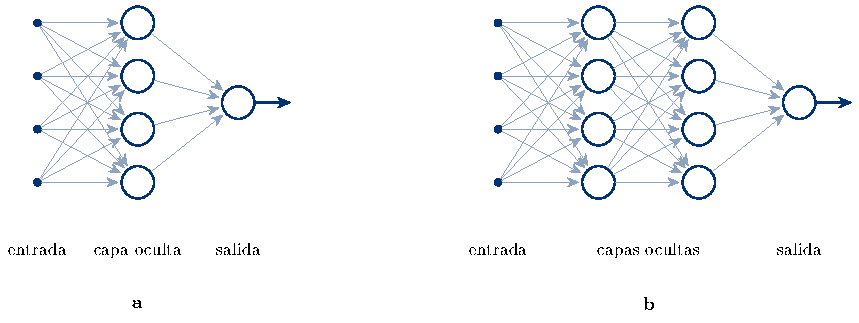
\includegraphics[max width=\linewidth]{Fig27.pdf}
\caption{{\bf a.} Una red neuronal con una capa escondida. {\bf b.} Una red neuronal con dos capas escondidas.}
\label{fig27}
\end{figure}

\subsection*{Capas} Notaremos el número de la capa con un índice $\ell$. Tenemos $\ell=0$ para la capa de entrada, $\ell=1$ para la primera capa escondida y $\ell=L$ para la capa de salida. Notemos que el número de capas escondidas es igual a $L-1$, El número de neuronas en la capa $\ell$ se nota por $d^{(\ell)}$. En particular, $d^{(0)}$ es el número de entradas y $d^{(L)}$ es el número de salidas.

\subsection*{Pesos} El sistema de pesos es denotado por $\{w_{ij}^{(\ell)}\}$, con $1\le \ell\le L$, $0\le i\le d^{(\ell-1)}$, $1\le j\le d^{(\ell)}$. El peso $w_{ij}^{(\ell)}$ se asocia al eje que conecta la $i-$ésima neurona de la capa $\ell-1$ con la $j-$ésima neurona de la capa $\ell$. Notemos que los ejes sólo conectan neuronas de capas consecutivas. Los pesos $w_{0j}^{(\ell)} = b_j^{(\ell)}$ son los sesgos y son los pesos correspondientes a las falsas entradas $x_0^{(\ell)} = -1$. El número de sesgos es igual al número de neuronas. El número de pesos, sin los sesgos, entre las capas $\ell-1$ y $\ell$ es dado por $d^{(\ell-1)}d^{(\ell)}$, con lo cual el número de pesos en una red de alimentación hacia adelante es 
$$
\sum_{\ell=1}^L  d^{(\ell-1)}d^{(\ell)}.
$$
Por ejemplo, la red de la figura \ref{fig27} {\bf a} tiene $4\times 4 + 4\times 1 = 20$ pesos, mientras que la de la figura \ref{fig27} {\bf b} tiene $4\times 4 +4\times 4 + 4\times 1 = 36$ pesos. Los pesos pueden ser tanto positivos, como negativos o incluso cero. Típicamente, un peso positivo estimula a la neurona a disparar, mientras que uno negativo la inhibe de hacerlo.

\subsection*{Entradas y salidas} Las entradas de la red se denotan por $x_j^{(0)}$, con $1\le j\le d^{(0)}$. Notamos por $x_j^{(\ell)}$ a la salida de la $j-$ésima neurona en la capa $\ell$. Luego, $x_j^{(L)}$ es la salida de la red, con $1\le j\le d^{(L)}$. Reservamos la notación $x_0^{(\ell)} = -1$ para las falsas entradas correspondientes a los sesgos de las neuronas de la capa $\ell+1$.

Consideremos la $j-$ésima neurona de la capa $\ell$.  En la primera parte, la neurona recoge la información de la capa previa como una suma ponderada en la señal
$$
s_j^{(\ell)} = \sum_{i=0}^{d^{(\ell-1)}} w_{ij}^{(\ell)} x_i^{(\ell-1)} = \sum_{i=1}^{d^{(\ell-1)}} w_{ij}^{(\ell)} x_i^{(\ell-1)} + b_j^{(\ell)}.
$$
En la segunda parte, la neurona aplica la función de activación $\varphi$ a la señal que recogió y produce el valor de salida
\begin{equation}\label{salida.neurona}
x_j^{(\ell)} = \varphi(s_j^{(\ell)}) = \varphi\left(\sum_{i=1}^{d^{(\ell-1)}} w_{ij}^{(\ell)} x_i^{(\ell-1)} + b_j^{(\ell)}\right).
\end{equation}
Esto puede escribirse en forma matricial como
$$
\xx^{(\ell)} = \varphi(W^{(\ell)^t} \xx^{(\ell-1)} + \bb^{(\ell)}),
$$
donde
$$
\xx^{(\ell)} = (x_1^{(\ell)},\dots, x_{d^{(\ell)}}^{(\ell)})^t, \quad W^{(\ell)} = \left( w_{ij}^{(\ell)}\right)_{i,j},\quad \bb^{(\ell)} = (b_1^{(\ell)},\dots, b_{d^{(\ell)}}^{(\ell)})^t,
$$
con $1\le i\le d^{(\ell-1)}$ y $1\le j\le d^{(\ell)}$ y hemos usado la convención de que la función de activación $\varphi$ aplicada a un vector actúa componente a componente. Observemos que la entrada de la red está dada por el vector $\xx^{(0)} =  (x_1^{(0)},\dots, x_{d^{(0)}}^{(0)})^t$ mientras que la salida es $ \xx^{(L)} = (x_1^{(L)},\dots, x_{d^{(L)}}^{(L)})^t$.

\subsection{Pasando a través de la red} Dado un sistema de pesos y sesgos, uno puede usar la ecuación \eqref{salida.neurona} para hallar las salidas de cada neurona en función de sus entradas. En particular uno encuentra la salida de la red, que es la salida de la última capa $\xx^{(L)}$. Avanzar a través de la red significa calcular todas las salidas de las neuronas. Este paso hacia adelante representa una etapa de predicción del objetivo. 

Esto prepara el terreno para la segunda etapa del método de recorrer la red hacia atrás para poder calcular el gradiente de la función de costo y así poder actualizar los parámetros fijados por el método de descenso de gradiente.

Estos pasajes hacia adelante y hacia atrás producen una sucesión de parámetros que corresponden a una sucesión de mejoras en la predicción del objetivo. Este proceso finaliza cuando la función de costo no puede mejorarse.

\subsection{Avanzando hacia atrás a través de la red}

Sea $C(w, b)$ la función de costo de la red, que mide la proximidad entre el objetivo $\zz$ y la salida $\yy=\xx^{(L)}$. Para poder aplicar el método de descenso de gradiente, necesitamos poder calcular precisamente el gradiente de $C$, $\nabla C = (\nabla_w C, \nabla_b C)$.

Dado que los pesos $w_{ij}^{(\ell)}$ conectan la $i-$ésima neurona en la capa $\ell-1$ con la $j-$ésima neurona de la capa $\ell$, el mismo va a entrar en el cálculo de la señal $s_j^{(\ell)}$ producida por la $j-$ésima neurona de la capa $\ell$. Más aún, ninguna otra señal de la capa $\ell$ se ve afectada por ese peso en particular. Luego, la regla de la cadena nos da
$$
\frac{\partial C}{\partial w_{ij}^{(\ell)}} = \frac{\partial C}{\partial s_j^{(\ell)}} \frac{\partial s_j^{(\ell)}}{\partial w_{ij}^{(\ell)}}.
$$
Usaremos la notación delta
$$
\delta_j^{(\ell)} = \frac{\partial C}{\partial s_j^{(\ell)}} 
$$
para notar la sensibilidad del error con respecto a la señal $s_j^{(\ell)}$. El segundo factor de la fórmula se calcula fácilmente como
$$
\frac{\partial s_j^{(\ell)}}{\partial w_{ij}^{(\ell)}} = x_i^{(\ell -1)},
$$
con lo que obtenemos
$$
\frac{\partial C}{\partial w_{ij}^{(\ell)}} = \delta_j^{(\ell)} x_i^{(\ell -1)}.
$$
Haciendo ahora un análisis similar, se calcula la derivada del costo con respecto a los sesgos y obtenemos
$$
\frac{\partial C}{\partial b_j^{(\ell)}} = \delta_j^{(\ell)}.
$$
De estas relaciones, obtenemos que el gradiente de $C$ se escribe como
$$
\frac{\partial C}{\partial w_{ij}^{(\ell)}}=\delta_j^{(\ell)}x_i^{(\ell -1)},\qquad \frac{\partial C}{\partial b_j^{(\ell)}}=\delta_j^{(\ell)},
$$
es decir, $\nabla C=(\nabla_w C, \nabla_b C)$ queda determinado por los deltas, de donde sigue que para el cálculo de $\nabla C$, sólo necesitamos calcular los deltas $\delta_j^{(\ell)}$.

Como vimos en el ejemplo de la sección previa, el cálculo de los deltas se realiza mediante un algoritmo de retropropagación que en el caso general lo discutiremos en la siguiente sección. 

\subsection{Retropropagación de los deltas}

Empecemos con el cálculo de los deltas en la última capa $\delta_j^{(L)}$, $1\le j\le d^{(L)}$. Esto depende esencialmente de la función de costo. Para simplificar los cálculos, asumamos que la función de costo viene dada por
$$
C(w, b) = \frac12 \sum_{j=1}^{d^{(L)}} (x_j^{(L)} - z_j)^2 = \frac12 \| \xx^{(L)} - \zz\|^2.
$$
Usando que $x_j^{(L)} = \varphi(s_j^{(L)})$, la regla de la cadena implica que
\begin{equation}\label{deltaL}
\delta_j^{(L)} = \frac{\partial C}{\partial s_j^{(L)}} = (x_j^{(L)}-z_j) \varphi'(s_j^{(L)}).
\end{equation}
Observemos que para algunas funciones de activación particulares, esta expresión puede simplificarse. Por ejemplo, para la función logística $\varphi=\sigma$, se tiene que $\sigma' = \sigma (1-\sigma)$ y para la función tangente hiperbólica $\varphi=\tb$ se tiene que $\tb' = (1-\tb^2)$, lo que evita el cálculo de $\varphi'$.


Ahora comienza la retropropagación. El objetivo es entonces calcular los deltas de la capa $\ell-1$ en función de los deltas de la capa $\ell$. Así, partiendo de la fórmula \eqref{deltaL} para los deltas de la última capa, podemos iterativamente calcular todos los deltas restantes.

Aplicamos una vez más la regla de la cadena y obtenemos
$$
\delta_i^{(\ell-1)} = \frac{\partial C}{\partial s_i^{(\ell-1)}} = \sum_{j=1}^{d^{(\ell)}} \frac{\partial C}{\partial s_j^{(\ell)}} \frac{\partial s_j^{(\ell)}}{\partial s_i^{(\ell-1)}} = \sum_{j=1}^{d^{(\ell)}}  \delta_j^{(\ell)}\frac{\partial s_j^{(\ell)}}{\partial s_i^{(\ell-1)}}.
$$
Debemos entonces calcular la derivada $\frac{\partial s_j^{(\ell)}}{\partial s_i^{(\ell-1)}}$, i.e. la sensibilidad de la señal en la capa $\ell$ con respecto a la señal en la capa previa. Recordemos que
$$
s_j^{(\ell)} = \sum_{i=1}^{d^{(\ell-1)}} w_{ij}^{(\ell)} x_i^{(\ell-1)} + b_j^{(\ell)} = \sum_{i=1}^{d^{(\ell-1)}} w_{ij}^{(\ell)} \varphi(s_i^{(\ell-1)}) + b_j^{(\ell)}, 
$$
de donde diferenciando con respecto a $s_i^{(\ell-1)}$, obtenemos
$$
\frac{\partial s_j^{(\ell)}}{\partial s_i^{(\ell-1)}} = w_{ij}^{(\ell)} \varphi'(s_i^{(\ell-1)}).
$$
Reemplazando en la expresión para el delta, obtenemos la {\em fórmula de retropropagación}
\begin{equation}\label{retro.delta}
\delta_i^{(\ell-1)} = \varphi'(s_i^{(\ell-1)})  \sum_{j=1}^{d^{(\ell)}}  \delta_j^{(\ell)} w_{ij}^{(\ell)}.
\end{equation}

En resumen, para calcular el gradiente de la función de costo, uno usa la fórmula de retropropagación \eqref{retro.delta} para calcular $\delta_i^{(\ell)}$ y la fórmula de propagación hacia adelante \eqref{salida.neurona} para el cálculo de las salidas $x_i^{(\ell-1)}$.

\subsection{Relaciones finales}
Los cálculos de las secciones previas se pueden resumir en el siguiente conjunto de {\em ecuaciones maestras}
\begin{align}
x_j^{(\ell)} &= \varphi\left(\sum_{i=1}^{d^{(\ell-1)}} w_{ij}^{(\ell)} x_i^{(\ell-1)} + b_j^{(\ell)}\right),\qquad 1\le j\le d^{(\ell)}\\
\delta_j^{(L)} &= (x_j^{(L)} - z_j)\varphi'(s_j^{(L)}),\qquad 1\le j\le d^{(L)}\\
\delta_i^{(\ell-1)} &= \varphi'(s_i^{(\ell-1)}) \sum_{j=1}^{d^{(\ell)}} \delta_j^{(\ell)} w_{ij}^{(\ell)},\qquad 1\le i\le d^{(\ell-1)}\\
\frac{\partial C}{\partial w_{ij}^{(\ell)}} &= \delta_j^{(\ell)} x_i^{(\ell-1)}\\
\frac{\partial C}{\partial b_j^{(\ell)}} &= \delta_j^{(\ell)}.
\end{align}
La primera de estas fórmulas nos da una expresión recursiva para el cálculo de las salidas en términos de los pesos y sesgos. La segunda nos da la expresión del delta de la capa de salida (suponiendo que la función de costo es la suma de los cuadrados de los errores). La tercera es la fórmula retropropagación de los deltas. Las últimas dos expresiones nos proveen las componentes del gradiente de $C$ con respecto a los pesos y sesgos.

\subsection{Forma matricial}
Para evitar confusiones con los índices es más conveniente reescribir las ecuaciones maestras de la sección anterior en forma matricial.

Para eso necesitamos introducir un nuevo producto entre vectores de la misma dimensión llamado el {\em producto de Hadamard}. Si $\uu$ y $\vv$ son vectores de $\R^n$ se define el producto de Hadamard de $\uu=(u_1,\dots, u_n)$ y $\vv=(v_1,\dots, v_n)$ como $\uu\odot\vv\in \R^n$ al vector con coordenadas $(\uu\odot\vv)_j = u_j v_j$. Es decir es el producto coordenada a coordenada. Su uso simplifica mucho la forma de las ecuaciones.

Usamos las notaciones
$$
\xx^{(\ell)} = (x_1^{(\ell)},\dots, x_{d^{(\ell)}}^{(\ell)})^t,\quad W^{(\ell)} = \left(w_{ij}^{(\ell)}\right)_{i,j},\quad \bb^{(\ell)} = (b_1^{(\ell)},\dots, b_{d^{(\ell)}}^{(\ell)})^t,
$$
$$
\delta^{(\ell)} = (\delta_1^{(\ell)},\dots, \delta_{d^{(\ell)}}^{(\ell)})^t,\quad \sbf^{(\ell)} = (s_1^{(\ell)},\dots, s_{d^{(\ell)}}^{(\ell)})^t
$$
junto con la convención de que $\varphi$ actúa sobre un vector componente a componente, las ecuaciones maestras de la sección anterior se pueden escribir como:
\begin{align}
\xx^{(\ell)} &= \varphi\left(W^{(\ell)^t} \xx^{(\ell-1)} + \bb^{(\ell)}\right)\\
\label{deltaL2}\delta^{(L)} &= (\xx^{(L)} - \zz)\odot \varphi'(\sbf^{(L)}) \\
\label{deltavec}\delta^{(\ell-1)} &= (W^{(\ell)}\delta^{(\ell)})\odot \varphi'(\sbf^{(\ell-1)}) \\
\label{partialC}\frac{\partial C}{\partial W^{(\ell)}} &= \xx^{(\ell-1)}\delta^{(\ell)^t} \\
\frac{\partial C}{\partial \bb^{(\ell)}} &= \delta^{(\ell)}.
\end{align}
Notemos que el lado derecho de \eqref{partialC} es una matriz resultado del producto de dos vectores. Más precisamente, si $\uu=(u_1,\dots, u_n)^t$ y $\vv=(v_1,\dots, v_n)^t$ son dos vectores columna en $\R^n$, entonces $\uu\vv^t = (u_iv_j)_{i,j}$ es una matriz de $n\times n$. Sin embargo, si se realiza el producto $\uu^t\vv = \sum_i u_i v_i$ es un escalar. Observemos también que en \eqref{deltavec} aparece $W^{(\ell)}$ y no la matriz transpuesta.

\begin{obs}
En el caso de una neurona lineal, las fórmulas previas pueden simplificarse. Dado que la función de activación es la identidad $\varphi(x)=x$, la fórmula de retropropagación para los delta se simplifica a $\delta^{(\ell-1)} = W^{(\ell)}\delta^{(\ell)}$. Iterando esta expresión, obtenemos
$$
\delta^{(\ell)} = W^{(\ell+1)}W^{(\ell+2)}\cdots W^{(L)}\delta^{(L)}.
$$
Luego, obtenemos las fórmulas
\begin{align*}
\frac{\partial C}{\partial W^{(\ell)}} &= \xx^{(\ell-1)}(W^{(\ell+1)}W^{(\ell+2)}\cdots W^{(L)}\delta^{(L)})^t\\
\frac{\partial C}{\partial \bb^{(\ell)}} &= -W^{(\ell+1)}W^{(\ell+2)}\cdots W^{(L)}\delta^{(L)},
\end{align*}
con lo que se obtiene una expresión explícita para el gradiente de la función de costo.
\end{obs}

\begin{obs}
La fórmula \eqref{deltaL2} está basada en la elección particular de la función de costo. En caso de que la función de costo se cambie, {\em solamente} hay que modificar la fórmula para $\delta^{(L)}$ que hay que ajustar acorde a ese cambio. Veamos un ejemplo con otra función de costo.
\end{obs}

\begin{ejem}
Supongamos que la función de costo es dada por la entropía cruzada
$$
C = -\sum_k z_k\ln x_k^{(L)} = -\sum_k z_k\ln \varphi(s_k^{(L)}),
$$
que representa la ineficiencia de usar la salida predecida $\xx^{(L)}$ en vez de el dato real $\zz$. El delta de la $j-$ésima neurona en la capa de salida es dada por
$$
\delta_j^{(L)} = \frac{\partial C}{\partial s_j^{(L)}} = -\frac{\partial}{\partial s_j^{(L)}} \sum_k z_k\ln \varphi(s_k^{(L)}) = -z_j \frac{\varphi'(s_j^{(L)})}{\varphi(s_j^{(L)})}.
$$

Esta expresión puede simplificarse aún más para algunas funciones de activación. Supongamos que $\varphi(x)=\sigma(x)$, entonces en este caso se tiene
$$
\delta_j^{(L)} =-z_j \frac{\sigma'(s_j^{(L)})}{\sigma(s_j^{(L)})} = -z_j\frac{\sigma(s_j^{(L)})(1-\sigma(s_j^{(L)}))}{\sigma(s_j^{(L)})} = -z_j (1-\sigma(s_j^{(L)})),
$$
que puede escribirse vectorialmente como
$$
\delta^{(L)} = - \zz\odot (1-\sigma(\sbf^{(L)})).
$$
Esta fórmula reemplaza \eqref{deltaL2} en este caso. Notemos que con sigmoides esta función de costo solo penaliza la clase verdadera; la entropía cruzada binaria completa, $C=-\sum_k[z_k\ln x_k^{(L)}+(1-z_k)\ln(1-x_k^{(L)})]$, da el delta mucho más simple $\delta^{(L)}=\xx^{(L)}-\zz$. Lo mismo ocurre con softmax y entropía cruzada: si $\xx^{(L)}=\softmax(\sbf^{(L)})$, $C=-\sum_kz_k\ln x_k^{(L)}$ y $\sum_kz_k=1$, entonces $\partial C/\partial s_j^{(L)}=x_j^{(L)}\sum_kz_k-z_j=x_j^{(L)}-z_j$. (Con softmax, $\varphi$ no actúa componente a componente, así que \eqref{deltaL} no vale.)
\end{ejem}

\subsection{El algoritmo de descenso de gradiente}

Consideremos una red neuronal con un sistema de pesos y sesgos iniciales dados por $w_{ij}^{(\ell)}(0)$ y $b_j^{(\ell)}(0)$. Estos pesos y sesgos pueden inicializarse eficientemente con un procedimiento que describiremos más adelante. Sea $\eta>0$ la tasa de aprendizaje. El valor óptimo de los pesos y sesgos luego de que la red es entrenada con el algoritmo de descenso de gradiente están dados por la sucesión aproximante definida por
\begin{align*}
w_{ij}^{(\ell)}(k+1) &= w_{ij}^{(\ell)}(k) - \eta \delta_j^{(\ell)}(k) x_i^{(\ell-1)}(k) \\
b_j^{(\ell)}(k+1) &= b_j^{(\ell)}(k) - \eta \delta_j^{(\ell)}(k),
\end{align*}
donde las salidas $x_i^{(\ell)}(k)$ y los deltas $\delta_j^{(\ell)}(k)$ dependen de los pesos $w_{ij}^{(\ell)}(k)$ y los sesgos $b_j^{(\ell)}(k)$ obtenidos en el $k-$ésimo paso.


\subsection{Definición formal de redes neuronales feedforward}

En esta sección daremos la definición matemática rigurosa de una red neuronal de propagación hacia adelante, o red neuronal {\em feedforward} (por su terminología en inglés).

Empecemos repasando los ingredientes usados hasta ahora en la construcción informal que hemos hecho. Hemos visto que una red neuronal feedforward contiene neuronas arregladas en $L+1$ capas distintas. La primera de esas capas corresponde a los datos de entrada se etiqueta con el superíndice $\ell=0$ y la capa de salida se etiqueta con $\ell=L$. La $j-$ésima neurona en la capa $\ell$ tiene activación $x_j^{(\ell)}$. Para la capa de entrada, $x_j^{(0)}$, las activaciones vienen como los datos de entrada, mientras que para las otras capas las activaciones se calculan en términos de las activaciones de las previas capas por la fórmula de propagación hacia adelante
$$
x_j^{(\ell)} = \varphi^{(\ell)}\left(\sum_{i=1}^{d^{(\ell-1)}} w_{ij}^{(\ell)} x_i^{(\ell-1)} + b_j^{(\ell)}\right),
$$
donde $\varphi^{(\ell)}$ es la función de activación de la capa $\ell$, $w_{ij}^{(\ell)}$ y $b_j^{(\ell)}$ son los pesos y sesgos de las neuronas en la capa $\ell$ respectivamente. Notemos también que la señal $s_j^{(\ell)} =\sum_{i=1}^{d^{(\ell-1)}} w_{ij}^{(\ell)} x_i^{(\ell-1)} + b_j^{(\ell)}$ es una función afín de $x_i^{(\ell-1)}$ y que la activación $x_j^{(\ell)}$ se obtiene de aplicar la función $\varphi^{(\ell)}$ a la señal $s_j^{(\ell)}$.

Realicemos ahora un nivel adicional de abstracción. (Identificamos $\F(U_\ell)$ con $\R^{d^{(\ell)}}$: así $f_\ell$ es el vector de activaciones $\xx^{(\ell)}$ y las funciones afines son de la forma $\xx\mapsto W^{(\ell)^t}\xx+ \bb^{(\ell)}$.) Notemos por $\F(U) = \{f\colon U\to\R\}$ el conjunto de todas las funciones a valores reales definidas sobre el conjunto $U$. Consideremos $U_\ell = \{1,\dots, d^{(\ell)}\}$ y definimos la función afín
$$
\alpha_\ell\colon \F(U_{\ell-1})\to \F(U_\ell)
$$
como $\alpha_\ell(\xx^{(\ell-1)}) = \sbf^{(\ell)}$. Luego $\xx^{(\ell)} = (\varphi^{(\ell)}\circ \alpha_\ell)(\xx^{(\ell-1)})$ se obtiene como la composición de la función afín en la capa de activación previa, con la nolinealidad $\varphi^{(\ell)}$.

La definición formal de una red neuronal feedforward es entonces la siguiente:
\begin{defi}
Consideremos $d^{(\ell)}\in\N$ con $\ell=0,\dots,L$ enteros positivos y $U_\ell =  \{1,\dots, d^{(\ell)}\}$. Sean $\alpha_1,\dots,\alpha_L$ funciones afines
$$
\alpha_\ell\colon \F(U_{\ell-1})\to \F(U_\ell)
$$
y sean $\varphi^{(\ell)}\colon \R\to\R$ funciones de activación. Entonces la correspondiente red neuronal feedforward es la sucesión de mapas $f_0, f_1,\dots, f_L$ dados por
$$
f_\ell = \varphi^{(\ell)}\circ\alpha_\ell\circ f_{\ell-1},\quad 1\le \ell\le L,
$$
donde $f_0$ es dada.
\end{defi}

Es decir, una red neuronal feedforward produce una sucesión de reparametrizaciones cada vez más abstractas $f_\ell$ que mapean la entrada $f_0$ a través de una seria de funciones paramétricas $\alpha_\ell$ y funciones de activación no lineales $\varphi^{(\ell)}$. La salida de la red es dada por
$$
f_L = \varphi^{(L)}\circ \alpha_L\circ \varphi^{(L-1)}\circ\alpha_{L-1}\circ\cdots\circ \varphi^{(1)}\circ \alpha_1\circ f_0.
$$
El número $L$ se lo denomina la {\em profundidad} de la red y a $\max\{d^{(1)},\dots, d^{(L)}\}$ (incluyendo la capa de salida) se lo llama anchura de la red.

Para problemas de regresión, la última función de activación es lineal $\varphi^{(L)}(x)=x$. Para problemas de clasificación, se suele tomar la función softmax, definida como
$$
\varphi^{(L)}(\xx) = \softmax(\xx) = \frac{1}{\sum_{i=1}^{d^{(L)}} e^{x_i}}(e^{x_1},\dots,e^{x_{d^{(L)}}}),
$$
(que no actúa componente a componente, a diferencia de lo supuesto antes) y en los casos de regresión logística la más usual es la sigmoideal $\varphi^{(L)}(x) = \sigma(x)$.

\section{Inicialización de los pesos}\label{sec.c6.3}

En el caso de redes con pocas capas, inicializar los pesos muestreándolos con una densidad uniforme o Gaussiana de media cero suele dar resultados satisfactorios. En cambio, inicializar todos los pesos con el mismo valor (en particular, con 0) no funciona: todas las neuronas de una capa reciben entonces el mismo gradiente, se actualizan igual y nunca se diferencian (problema de simetría); por eso la inicialización debe ser aleatoria. Sin embargo, en el caso de redes neuronales profundas con un gran número de capas es necesario inicializar los pesos con cuidado dado que ese proceso tiene mucha importancia en el funcionamiento del algoritmo de minimización.

La magnitud de los pesos juega un rol importante en evitar tanto como sea posible el problema de gradiente pequeño o muy grande. Esto será descripto en las siguientes dos situaciones marginales.

\begin{enumerate}
\item {\em Si los pesos están muy cerca de cero, entonces la varianza de la entrada decrece mientras pasa por cada capa de la red}.

Este enunciado heurístico está basado en el siguiente cálculo: sea $x_j^{(\ell)}$ la salida de la $j-$ésima neurona en la capa $\ell$. Las salidas entre dos capas consecutivas está dado por la ecuación de propagación
$$
x_j^{(\ell)} = \varphi\left(\sum_i w_{ij}^{(\ell)} x_i^{(\ell-1)} + b_j^{(\ell)}\right),
$$
Queremos ahora calcular la varianza de esta salida, $\V[x_j^{(\ell)}]$.

Para este cálculo, observemos que si $X$ es una variable aleatoria y llamemos $m=\E[X]$. Si $f$ es una función de clase $C^2$, entonces tenemos que
$$
f(x) = f(m) + f'(m) (x-m) + O(|x-m|^2),
$$
de donde obtenemos la aproximación
$$
f(X) \simeq f(m) + f'(m)(X-m).
$$
Tomando varianza a ambos lados llegamos a la fórmula
\begin{equation}\label{var}
\V[f(X)] \simeq f'(m)^2 \V[X]
\end{equation}

Usando ahora esta aproximación para la varianza y asumiendo que las variables $x_i^{(\ell-1)}$ son independientes entre sí (hipótesis heurística, ya que en general dependen de la misma entrada), calculamos
$$
\V[x_j^{(\ell)}] \simeq \left[\varphi'\left(\sum_i w_{ij}^{(\ell)} x_i^{(\ell-1)} + b_j^{(\ell)}\right)\right]^2 \sum_i \left(w_{ij}^{(\ell)}\right)^2 \V[x_i^{(\ell-1)}].
$$
Esta expresión nos da la varianza de las neuronas en la capa $\ell$ en término de las varianzas de las neuronas en la capa previa.

Ahora realicemos la siguiente estimación. Asumamos primero que la función de activación tiene derivada acotada, i.e. $|\varphi'|^2\le C$ y usando la desigualdad de Cauchy obtenemos
$$
\begin{aligned}\V[x_j^{(\ell)}]&\le C\sum_i (w_{ij}^{(\ell)})^2 \V[x_i^{(\ell-1)}]\le C \left(\sum_i (w_{ij}^{(\ell)})^4\right)^{1/2} \left(\sum_i (\V[x_i^{(\ell-1)}])^2\right)^{1/2}\\&\le C \left(\sum_i (w_{ij}^{(\ell)})^2\right) \left(\sum_i (\V[x_i^{(\ell-1)}])^2\right)^{1/2}.\end{aligned}
$$
Finalmente, elevamos al cuadrado y sumamos sobre $j$ para obtener
$$
\sum_j(\V[x_j^{(\ell)}])^2 \le C^2 \sum_j\Big(\sum_i (w_{ij}^{(\ell)})^2\Big)^2 \sum_i (\V[x_i^{(\ell-1)}])^2\le C^2 \Big(\sum_{i,j} (w_{ij}^{(\ell)})^2\Big)^2 \sum_i (\V[x_i^{(\ell-1)}])^2.
$$
Esto muestra que si los pesos son pequeños (si $C\sum_{i,j}(w_{ij}^{(\ell)})^2<1$), entonces la varianza de la capa $\ell$ es más pequeña que la de la capa previa. Iterando la desigualdad, sigue que la varianza de la señal decae a 0 luego de pasar por un cierto número de capas con lo que la variación de la señal se vuelve insignificante.

\bigskip

\item {\em Si los pesos son muy grandes, entonces la varianza de la señal tiende a amplificarse cuando pasa por las capas de la red, o las activaciones saturan y la red entra en una zona de gradiente casi nulo (un {\em plateau})}.

En este caso, si los pesos $w_{ij}^{(\ell)}$ son grandes, entonces la suma $\sum_i w_{ij}^{(\ell)} x_i^{(\ell-1)}$ también es grande.

Supongamos que la función de activación es lineal, $\varphi(x)=x$, entonces
$$
\V[x_j^{(\ell)}] = \sum_i \left(w_{ij}^{(\ell)}\right)^2 \V[x_i^{(\ell-1)}],
$$
lo que implica que la varianza $\V[x_i^{(\ell)}]$ también se vuelve grande.

Supongamos que la función de activación es sigmoide, entonces en ese caso la función $\sigma$ se vuelve saturada y por ende $\sigma'$ es muy pequeño, lo que trae el problema de gradiente cercano a cero.
\end{enumerate}

Luego, para que la inicialización sea viable, es necesario que los pesos no sean ni muy grandes ni muy pequeños. Necesitamos que la inicialización sea en un rango {\em razonable} antes de iniciar el entrenamiento de la red. Veremos ahora cómo tratar con este problema.

La idea principal se basa en el hecho de que la propagación del error de la señal a través de una red neuronal profunda puede cuantificarse mediante la varianza de la señal, es decir, la varianza de las activaciones de las neuronas. Para mantener la varianza bajo control, evitando valores que se disparen o se anulen, la forma más simple es encontrar valores de los pesos para los cuales la varianza se mantenga aproximadamente constante al pasar la señal por cada capa. Dado que la asignación de los pesos iniciales es un proceso aleatorio, asumimos que los pesos son variables aleatorias con distribución uniforme o Gaussiana y media cero.

Simplifiquemos la notación levemente. Fijemos una capa $\ell$ y notamos al vector de entrada de esa capa como $X=X^{(\ell-1)}$ (usamos la notación de letras mayúsculas dado que serán todos variables aleatorias) y al vector de salida de la capa como $Y=X^{(\ell)}$. El número de neuronas lo notaremos como $N=d^{(\ell-1)}$. La $j-$ésima componente de $Y$ está dada por
$$
Y_j = \varphi\left(\sum_i W_{ij} X_i + b_j\right),
$$
donde la matriz de pesos $W_{ij}$ es una matriz aleatoria con media cero. Sobre los $X_i$ asumimos que son independientes, idénticamente distribuidos y con media 0 (por ejemplo pueden ser Gaussianos o con distribución uniforme). Asumamos también que $W_{ij}$ y $X_i$ son independientes. Sobre los sesgos $b_j$ asumimos que son constantes (usualmente se inicializan como 0). 

Ahora, usando la fórmula de aproximación para la varianza dada por \eqref{var}, obtenemos
\begin{align*}
\V[Y_j] &\simeq \varphi'\left(\sum_i \E[W_{ij} X_i] + b_j\right)^2 \V\left[\sum_i W_{ij} X_i\right]\\
&= \varphi'(b_j)^2 \sum_i \V[W_{ij}X_i] = \varphi'(b_j)^2 \sum_i \V[W_{ij}] \V[X_i]\\
&= N\varphi'(0)^2 \V[W_{11}] \V[X_1],
\end{align*}
donde hemos usado que $\E[W_{ij}X_i] = \E[W_{ij}]\E[X_i] = 0$ por la independencia de las variables en la segunda igualdad, que $\V[WX] = \V[W]\V[X]$ para variables aleatorias independientes con media cero en la tercer igualdad y que las variables aleatorias son idénticamente distribuidas (y tomamos $b_j=0$) para la última igualdad.

Si requerimos que la varianza no se modifique en el paso de capa a capa, esto equivale a pedir que $\V[Y_j] \simeq \V[X_i]$, luego obtenemos
$$
N\varphi'(0)^2 \V[W_{11}] \V[X_1] \simeq \V[X_1].
$$
Simplificando obtenemos la expresión para la varianza de los pesos
$$
\V[W_{ij}] = \V[W_{11}] \simeq \frac{1}{N\varphi'(0)^2}.
$$

Tenemos dos casos importantes
\begin{enumerate}
\item Los pesos tienen una distribución normal $W_{ij}\sim N(0,\tfrac{1}{N\varphi'(0)^2})$. En particular, si la función de activación es lineal, $\varphi'(0)=1$ y en ese caso $W_{ij}\sim N(0,\tfrac{1}{N})$.

\item Los pesos tienen una distribución uniforme $W_{ij}\sim U([-a,a])$ para $a>0$. En este caso, igualando las varianzas obtenemos
$$
\frac{1}{N\varphi'(0)^2} = \frac{a^2}{3}, \quad \text{de donde}\quad a=\frac{\sqrt 3}{\varphi'(0)\sqrt{N}}.
$$
Notemos que la pendiente de la función de activación en el origen afecta el rango del intervalo en donde debemos tomar los valores de los pesos. Mientras más grande sea esa pendiente, más angosto debe ser ese intervalo. Una forma de utilizar este hecho es considerar la escala de los pesos como un hiperparámetro y ajustarla en un conjunto de validación.
\end{enumerate}

Este análisis supone que las entradas de cada capa tienen media cero y que $\varphi$ es derivable en $0$ con $\varphi'(0)\ne0$: vale para la tangente hiperbólica ($\varphi'(0)=1$, de donde $\V[W]=1/N$, la inicialización de LeCun), pero no para la logística ni para la ReLU, cuyas salidas no tienen media cero. Para la ReLU (que no es derivable en $0$) el análisis análogo da $\V[W]=2/N$ (inicialización de He et al., 2015). Si se tiene en cuenta además la propagación hacia atrás, Glorot y Bengio (2010) proponen $\V[W]=2/(d^{(\ell-1)}+d^{(\ell)})$.


\section{Resumen}\label{sec.c6.4}

Una red neuronal es obtenida por una concatenación de varias capas de neuronas. La primera capa corresponde con las entradas y la última con la salida. Las capas intermedias se llaman capas ocultas. Este capítulo trató sólo de las llamadas {\em redes feedforward}. Estas son redes en donde la información fluye hacia adelante desde la entrada a la salida.

Las redes neuronales son usadas para aprender características complejas, que una única neurona no es capaz de hacer. Las redes son entrenadas por el método de descenso de gradiente. Un ingrediente importante de este método es el cálculo del gradiente de la función de costo. Este gradiente es calculado por un método recursivo llamado retropropagación. Las ecuaciones maestras tanto para la propagación hacia adelante, como para la retropropagación son analizadas en detalle.

Para que el método de descenso de gradiente funcione adecuadamente, es necesario dar valores iniciales a los pesos y sesgos. Los pesos se inicializan al azar, con media cero, para romper la simetría entre neuronas (inicializarlos todos en cero haría que las neuronas de una capa evolucionen de manera idéntica); cuando la red es profunda, es necesario además desarrollar ciertas estrategias para elegir la escala de esa inicialización.

\section{Ejercicios}\label{sec.c6.5}

\begin{ejer}
Dibujar el esquema de la red dada por la Observación \ref{obsXOR}.
\end{ejer}

\begin{ejer}
\begin{itemize}
\item[(a)] ¿Puede un único perceptrón aprender el siguiente mapa:
$$\begin{array}{llll}
(0,0,0)\mapsto 1, & (1,0,0)\mapsto 0, & (0,1,0)\mapsto 0, & (0,0,1)\mapsto 0,\\
(0,1,1)\mapsto 1, & (1,1,0)\mapsto 0, & (1,0,1)\mapsto 0, & (1,1,1)\mapsto 1?
\end{array}
$$

\item[(b)] Dibujar el esquema de una red neuronal con perceptrones que aprenda el mapa del ítem anterior. Dar los pesos y sesgos de todos los perceptrones de la red.
\end{itemize}
\end{ejer}

\begin{ejer}\label{ej663}
Escribir una fórmula explícita para la salida de la red neuronal multi-perceptrón dada por la figura \ref{fig28} {\bf a}.
\end{ejer}

\begin{figure}[htbp]
\centering
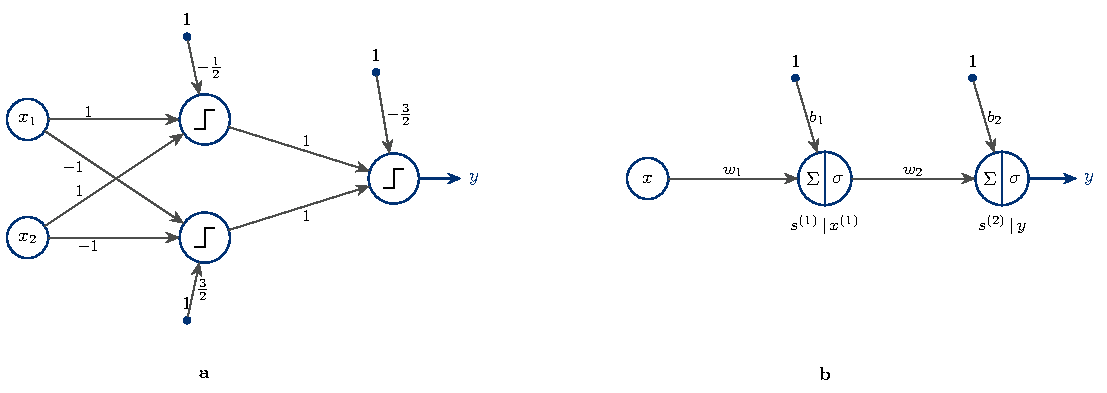
\includegraphics[max width=\linewidth]{Fig28.pdf}
\caption{{\bf a.} La red neuronal usada en le Ejercicio \ref{ej663}. {\bf b.} La red neuronal usada en el Ejercicio \ref{ej666}.}
\label{fig28}
\end{figure}

\begin{ejer}
Considerar una neurona sigmoide con una entrada unidimensional $x$, peso $w$, sesgo $b$ y salida $y=\sigma(wx+ b)$. El objetivo es una variable unidimensional $z$. Consideremos la función de costo $C(w, b) = \tfrac12 (y-z)^2$.
\begin{itemize}
\item[(a)] Hallar $\nabla C(w, b)$ y mostrar que $\|\nabla C(w, b)\| < \tfrac14 \sqrt{1+x^2} (1+|z|)$.

\item[(b)] Escribir la iteración de descenso de gradiente para la sucesión de pesos $(w_n, b_n)$.
\end{itemize}
\end{ejer}

\begin{ejer}\label{ej666}
Consideremos la red neuronal dada por la figura \ref{fig28} {\bf b}, con la función de costo dada por $C(w, b)= \tfrac12 (y-z)^2$.
\begin{itemize}
\item[(a)] Calcular las deltas $\delta^{(\ell)} = \tfrac{\partial C}{\partial s^{(\ell)}}$, $\ell=1, 2$.
\item[(b)] Usar el algoritmo de retropropagación para hallar el gradiente $\nabla C(w, b)$.
\end{itemize}
\end{ejer}

\begin{ejer}
Asumamos que la función de activación en la capa $\ell$ es lineal y que los pesos y entradas son variables aleatorias.
\begin{itemize}
\item[(a)] Mostrar que $\delta^{(\ell)}=W^{(\ell+1)}\cdots W^{(L)}\delta^{(L)}$ no depende de $W^{(\ell)}$ ni de $X^{(\ell-1)}$ más que a través de $\delta^{(L)}$.
\item[(b)] Concluir que, si $W^{(\ell+1)},\dots,W^{(L)},\delta^{(L)}$ son independientes de $W^{(\ell)}$ y de $X^{(\ell-1)}$, entonces $\delta_j^{(\ell)}$ es independiente de $W_{ij}^{(\ell)}$ y de $X_i^{(\ell-1)}$. (Esta hipótesis es solo una aproximación, ya que $\delta^{(L)}$ depende de la salida de la red, que sí depende de $W^{(\ell)}$ y de $X^{(\ell-1)}$.)
\end{itemize}
\end{ejer}

\begin{ejer}
Considerar una neurona sigmoide con entrada aleatoria normalmente distribuida, $X\sim N(0,1)$ y con salida $Y=\sigma(wX+ b)$. Mostrar que $\V[Y] \simeq w^2 \sigma'(b)^2$. Notar que la varianza de la salida decrece para valores pequeños del peso $w$ o grandes valores del sesgo $|b|$.
\end{ejer}

\begin{ejer}
Considerar una red neuronal con una capa escondida que posee neuronas sigmoides en esa capa. Suponer que las entradas están normalmente distribuidas, $X\sim N(0,1)$ y que la salida es $Y=\sum_{i=1}^N \alpha_i \sigma(w_i X + b_i)$. Mostrar que $\V[Y]\simeq \Bigl(\sum_{i=1}^N \alpha_i\,\sigma'(b_i)\, w_i\Bigr)^2$ (todos los sumandos dependen de la misma $X$, así que no son independientes).
\end{ejer}

\part{Teoría analítica}

%%%%%%%%%%%%%%%%%%%%%%%%%%%%%%%%%%%%%%%%
%% CAPITULO 7 %%%%%%%%%%%%%%%%%%%%%%%%%%%%%%%
%%%%%%%%%%%%%%%%%%%%%%%%%%%%%%%%%%%%%%%%

\chapter{Teoremas de aproximación}

Este capítulo presenta algunos resultados clásicos del análisis real con aplicaciones al aprendizaje de funciones continuas, integrables o de cuadrado integrables. Los resultados de aproximación incluidos en este capítulo abarcan el teorema de Dini, el teorema de Arzelà-Ascoli, el teorema de Stone-Weierstrass, el teorema tauberiano de Wiener y el principio de contracción. Algunas de sus aplicaciones al aprendizaje se proporcionarán dentro de este capítulo, mientras que otras se presentarán en capítulos posteriores.

Este capítulo reúne las herramientas de análisis que se usan en los siguientes: el teorema de Dini (Sección~\ref{sec.c7.1}), el de Arzelà--Ascoli (Sección~\ref{sec.c7.2}), el de Stone--Weierstrass (Sección~\ref{sec.c7.3}), los teoremas tauberianos de Wiener (Sección~\ref{sec.c7.4}) y el principio de contracción (Sección~\ref{sec.c7.5}). Corresponde al Capítulo~7 de~\cite{Calin}.

\section{El Teorema de Dini}\label{sec.c7.1}

Aprender una función continua en un intervalo compacto se reduce a demostrar que la red neuronal produce una secuencia de funciones continuas que converge uniformemente a la función objetivo continua. En la mayoría de los casos, no es difícil construir resultados que converjan puntualmente a la función objetivo. Sin embargo, demostrar la convergencia uniforme puede ser, a veces, una tarea complicada. En ciertas circunstancias, esto puede simplificarse mediante el uso de algunos resultados de aproximación, como los siguientes.

\begin{teo}[Dini]\label{teoDini}
Sea $f_n\colon [a, b]\to \R$ una sucesión de funciones continuas.
\begin{itemize}
\item[(a)]\label{Dini-a} Si $f_{n+1}\le f_n$ para $n\ge 1$ y $f_n(x)\to 0$ puntualmente para $x\in [a, b]$, entonces $f_n$ converge uniformemente a 0 en $[a, b]$.

\item[(b)]\label{Dini-b} Si $g\in C([a, b])$ es tal que $f_n(x)\searrow g(x)$ puntualmente para $x\in [a, b]$, entonces $f_n$ converge uniformemente a $g$ en $[a, b]$.
\end{itemize}
\end{teo}

\begin{proof}
El ítem (b) se obtiene aplicando (a) a la sucesión $f_n-g$. Veamos la demostración de (a).

Sea $\ve>0$ y consideremos los conjuntos
$$
A_n(\ve) = f_n^{-1}([\ve, \infty)) = \{x\in [a, b]\colon f_n(x)\ge \ve\}.
$$
Como $f_n$ decrece puntualmente a $0$, se tiene $f_n\ge 0$; por lo tanto, lo que queremos ver, que $f_n\rightrightarrows 0$, es equivalente a probar que existe $N\in\N$ tal que $A_n(\ve)=\emptyset$ para $n\ge N$.

Como las funciones $f_n$ son continuas, entonces los conjuntos $A_n(\ve)$ son cerrados. Más aún, como $A_n(\ve)\subset [a, b]$, resultan compactos. Adicionalmente, como $\{f_n\}_{n\in\N}$ es decreciente, los conjuntos $A_n(\ve)$ están encajados, i.e. $A_{n+1}(\ve)\subset A_n(\ve)$ para $n\in \N$. Supongamos que $A_n(\ve)\neq\emptyset$ para todo $n\ge 1$. Entonces, tenemos que $\cap_{n\ge 1} A_n(\ve)\neq\emptyset$ por ser la intersección de una sucesión de conjuntos compactos encajados. Pero si $x_0\in \cap_{n\ge 1} A_n(\ve)$, entonces $f_n(x_0)\ge \ve$ para todo $n\in\N$ lo que contradice el hecho de que $f_n(x_0)\to 0$ cuando $n\to\infty$.
\end{proof}

\begin{obs}
El Teorema de Dini sigue siendo cierto si se reemplaza el intervalo $[a, b]$ por un espacio métrico compacto $(S, d)$ y la convergencia es considerada respecto de la métrica $d$.
\end{obs}

\begin{ejem}
Sea $g\colon [0,1]\to\R$ de clase $C^2$ con finitos puntos de inflexión y consideremos la partición $\Delta_1$ dada por $0=x_0<x_1<\cdots<x_n=1$, donde $x_1,\dots,x_{n-1}$ son los puntos de inflexión de $g$. Es decir, $g|_{[x_{i-1}, x_i]}$ es cóncava o convexa para todo $i=1,\dots,n$. Notemos por $f_1$ a la función lineal a trozos que se obtiene de unir a los puntos $(x_i, g(x_i))$, $i=0,\dots,n$. 

Consideremos ahora la partición $\Delta_2$ que consiste en agregar a $\Delta_1$ los puntos medios de cada subintervalo, y notemos a la nueva función lineal a trozos que une los puntos dados por la partición $\Delta_2$ como $f_2$.

Si continuamos con este proceso, obtenemos una sucesión de particiones $\Delta_n$ y una sucesión de funciones lineales a trozos $f_n$. Esta sucesión, verifica la propiedad
$$
|g(x)-f_{n+1}(x)|\le |g(x)-f_n(x)|,\quad \forall x\in [0,1].
$$
En efecto, en cada intervalo donde $g$ es convexa (cóncava) se tiene $f_n\ge g$ ($f_n\le g$), y al refinar la partición la poligonal se acerca a $g$ sin cruzarla. Además $f_n(x)\to g(x)$ para todo $x$, pues el tamaño de la partición tiende a $0$ y $g$ es continua. Luego $|g-f_n|$ es una sucesión decreciente de funciones continuas que tiende a $0$ puntualmente, y el Teorema de Dini, Teorema \ref{teoDini}, implica que $f_n$ converge a $g$ uniformemente en $[0,1]$. (Aquí la convergencia uniforme también se deduce directamente de la continuidad uniforme de $g$; el ejemplo ilustra cómo la monotonía, que muchas veces es fácil de verificar, permite pasar de convergencia puntual a uniforme.)
\end{ejem}

\section{Teorema de Arzela-Ascoli}\label{sec.c7.2}
Otro resultado para construir una sucesión que converja uniformemente, es extraer de una sucesión dada, una subsucesión que tenga esa propiedad. El Teorema de Arzela-Ascoli nos provee de este resultado de existencia. Al ser un resultado teórico y no constructivo, tiene implicancias importantes teóricas y no en la construcción de algoritmos.

Necesitamos unas definiciones para poder enunciar el teorema. Una familia de funciones $\F$ definidas sobre un conjunto $A$ a valores reales se dice {\em uniformemente acotada} si existe $M>0$ tal que
$$
|f(x)|\le M,\qquad \forall x\in A,\quad \forall f\in \F.
$$

\begin{ejem}\label{ej7.2.2}
Por ejemplo, la familia
$$
\F = \left\{ \sum_{j=1}^N \alpha_j \sigma(w_j x + b_j)\colon \alpha_j, w_j, b_j\in\R,\ \sum_{j=1}^N \alpha_j^2 \le 1\right\},
$$
donde $\sigma(x)$ es una función sigmoidea tal que $|\sigma(x)|\le 1$ resulta ser uniformemente acotada. 

En efecto, si llamamos $\alpha = (\alpha_1,\dots,\alpha_N)$ y $\bar\sigma(x) = (\sigma(w_1 x+b_1),\dots, \sigma(w_N x+b_N))$, usando la desigualdad de Cauchy-Schwartz, tenemos
$$
\left|\sum_{j=1}^N \alpha_j \sigma(w_j x + b_j)\right| = |\alpha\cdot \bar\sigma(x)|\le \|\alpha\| \|\bar\sigma(x)\| \le 1\cdot \sqrt{N} = \sqrt{N}.
$$
\end{ejem}

Una familia de funciones $\F$ definidas en un conjunto $A\subset \R^n$ se dice {\em equicontinua}, si para todo $\ve>0$, existe $\delta>0$ tal que para toda $f\in\F$ se verifica que
$$
|f(x)-f(y)|<\ve,\quad \forall x, y\in A \text{ con } |x-y|<\delta.
$$

El ejemplo más importante de una familia de funciones equicontinua es un conjunto de funciones de clase $C^1$ con derivada acotada. En efecto, supongamos que tenemos una familia $\F\subset C^1([a, b])$ y que existe $L>0$ tal que
$$
\sup_{x\in [a, b]} |f'(x)|\le L,\qquad \forall f\in \F.
$$
Luego, usando el Teorema del valor medio, obtenemos
$$
|f(x)-f(y)| = |f'(\xi) (x-y)|\le \sup_{\xi\in [a, b]}|f'(\xi)| |x-y|\le L|x-y|,
$$
de donde tomando $\delta = \ve/L$ obtenemos lo deseado.

\begin{ejem}\label{ej7.2.4}
Consideremos la familia
$$
\F = \left\{\sum_{j=1}^N \alpha_j \sigma(w_j x + b_j)\colon \alpha_j, w_j, b_j\in\R,\ \sum_{j=1}^N (\alpha_j^2 + w_j^2) \le 1\right\},
$$
donde $\sigma$ verifica  que $|\sigma'|\le \lambda$. Entonces $\F$ es equicontinua. En efecto, si $f\in \F$, tenemos que
\begin{align*}
|f'(x)| &= \left|\sum_{j=1}^N \alpha_j w_j\sigma'(w_j x+b_j)\right|\le \lambda\sum |\alpha_j||w_j|\\
&\le \lambda\sum_{j=1}^N \frac{\alpha_j^2 + w_j^2}{2} \le \frac{\lambda}{2}.
\end{align*}
Luego, por lo visto en el párrafo anterior, $\F$ resulta equicontinua.
\end{ejem}

Tenemos entonces el teorema
\begin{teo}[Arzela-Ascoli]  
Sea $K\subset \R^n$ un conjunto compacto y $\F\subset C(K)$ una familia de funciones continuas. Son equivalentes:
\begin{itemize}
\item[(a)] Toda sucesión $\{f_n\}_{n\in\N}\subset \F$ contiene una subsucesión $\{f_{n_k}\}_{k\in\N}\subset \{f_n\}_{n\in\N}$ que es uniformemente convergente.
\item[(b)] La familia $\F$ es equicontinua y uniformemente acotada.
\end{itemize}
\end{teo}

La demostración de este teorema se suele dar tanto en el curso de Cálculo Avanzado como en el de Análisis Avanzado y lo pueden encontrar en el libro \cite{Royden}.

Como aplicación del Teorema de Arzela-Ascoli, veamos un resultado de existencia. Si se restringen el tamaño de la capa oculta, la pendiente de la función de activación y el tamaño de los pesos, el conjunto de las funciones que produce una red de tres capas es {\em relativamente compacto} en $C([a,b])$: toda sucesión de redes admite una subsucesión que converge uniformemente a alguna función continua.

\begin{teo}
Sea $N\ge 1$ un entero fijo y consideremos una red neuronal con una capa oculta de manera tal que se verifican:
\begin{itemize}
\item[(a)] La entrada de la red es una variable real acotada $x\in [a, b]$.
\item[(b)] La salida de la red es una neurona unidimensional con una función de activación lineal y sin sesgo.
\item[(c)] Tenemos $N$ neuronas en la capa oculta con una función de activación $\sigma$ que es derivable y tal que $|\sigma|\le 1$ y $|\sigma'|\le \lambda$.
\item[(d)] Los pesos satisfacen la condición $\sum_{j=1}^N (\alpha_j^2 + w_j^2) \le 1$, donde $w_j$ son los pesos de entrada a la capa oculta y $\alpha_j$ son los pesos que conectan la capa oculta con la salida.
\end{itemize}
Entonces la familia $\F$ de todas las salidas posibles de la red es relativamente compacta en $C([a,b])$: toda sucesión $\{f_n\}\subset\F$ posee una subsucesión que converge uniformemente en $[a,b]$ a una función $g\in C([a,b])$.
\end{teo}

\begin{proof}
La función de salida de la red viene dada por la suma
$$
f_{\alpha, w, b}(x) = \sum_{j=1}^N \alpha_j \sigma(w_j x + b_j),
$$
donde $w_j$ son los pesos de la entrada a la capa oculta y $\alpha_j$ son los pesos de la capa oculta a la salida. Los sesgos son notados por $b_j$. La restricción sobre los pesos del ítem (d), implican que la familia $\F=\{f_{\alpha, w, b}\colon \alpha, w, b\in \R^N,\ \sum_{j=1}^N(\alpha_j^2+w_j^2)\le1\}$ es uniformemente acotada (ver el Ejemplo \ref{ej7.2.2}; aquí se usa $|\sigma|\le1$). Por lo visto en el Ejemplo \ref{ej7.2.4}, la familia $\F$ resulta también equicontinua.

Luego, podemos aplicar el Teorema de Arzela-Ascoli y concluir que toda sucesión de salidas $\{f_n\}_{n\in\N}\subset \F$ dada por
$$
f_n(x) = \sum_{j=1}^N \alpha_j(n) \sigma(w_j(n) x + b_j(n)),
$$
posee una subsucesión $\{f_{n_k}\}_{k\in\N}\subset \{f_n\}_{n\in\N}$ que es uniformemente convergente en $[a, b]$ y su límite es una cierta función continua $g\in C([a, b])$.
\end{proof}

\begin{obs}
En el resultado anterior, la función continua $g$ no es conocida a priori y no tiene por qué ser una función objetivo dada: de cualquier sucesión infinita de redes admisibles (por ejemplo, de intentos de entrenamiento) se puede extraer una subsucesión que converge uniformemente a alguna función continua. Esto es un resultado de existencia; construir la subsucesión convergente es un problema diferente. Notemos además que el resultado no dice que cualquier función continua pueda aproximarse: la restricción (d) hace que la clase de funciones representables sea relativamente compacta y, por lo tanto, {\em no} densa en $C([a,b])$. La aproximación de funciones arbitrarias (sin restricciones sobre el tamaño de los pesos ni de $N$) es el tema del Capítulo~\ref{cap9}.
\end{obs}

\begin{ejem}[Neurona sigmoidal]
Consideremos una neurona sigmoidal con salida 
$$
f_{\ww, b}(\xx) = \sigma(\ww\cdot\xx + b),
$$
donde $\sigma$ es la función logística, con pesos $\ww\in \R^n$, sesgo $b\in \R$ y entrada $\xx\in I_n = [0,1]\times\cdots\times[0,1]\subset \R^n$.

Asumamos que los pesos son acotados con $\|\ww\|\le 1$. Entonces la familia de funciones continuas
$$
\F=\{ f_{\ww, b}\colon \|\ww\|\le 1,\ b\in \R\},
$$
es uniformemente acotada (pues $\sup |f_{\ww, b}| \le \sup |\sigma|=1$) y equicontinua, pues si $f\in \F$, como $0<\sigma'\le\frac14$,
$$
\|\nabla f(\xx)\| = |\sigma'(\ww\cdot\xx + b)|\,\|\ww\|\le \tfrac14,
$$
de modo que, por el teorema del valor medio en el conjunto convexo $I_n$, $|f(\xx)-f(\yy)|\le \frac14\|\xx-\yy\|$ para toda $f\in\F$.
Luego, por el Teorema de Arzela-Ascoli, toda sucesión de salidas $\{f_{\ww_k, b_k}\}_{k\in\N}$ contiene una subsucesión uniformemente convergente a una función continua $g$ definida en $I_n$. Observemos que no se hacen hipótesis sobre los sesgos.
\end{ejem}

\subsection{Aplicaciones a redes neuronales}\label{sec.7.3}

Las nociones anteriores pueden aplicarse al estudio de redes neuronales de una capa oculta con un continuo de neuronas en la capa oculta; ver también la sección \ref{sec.5.8}.

Supongamos que la entrada pertenece a un intervalo compacto, $x \in [a, b]$. Es bien sabido que una red neuronal de una capa oculta, con $N$ neuronas en la capa oculta, tiene una salida dada por  
$$
g(x) = \sum_{j=1}^{N} \sigma(w_j x + b_j) \alpha_j,
$$
donde $\sigma$ es una sigmoide logística. Además, $w_j$ son los pesos entre la entrada y la $j-$ésima neurona, $\alpha_j$ es el peso entre la $j-$ésima neurona y la salida, y $b_j$ denota el sesgo de la $j-$ésima neurona en la capa oculta.

Queremos generalizar al caso en que el número de unidades ocultas es infinito. En particular, queremos considerar el caso en que el número de unidades ocultas es {\em infinitamente numerable}. Suponemos que las neuronas ocultas están parametrizadas de forma continua por $t$, tomando valores en el compacto $[c, d]$. De este modo, el parámetro $t$ reemplazará al índice $j$.  

Además, los pesos de suma $\alpha_j$ serán reemplazados por una medida, que bajo la hipótesis de ser absolutamente continua con respecto a la medida de Lebesgue $dt$ en $[c,d]$, tomará la forma $h(t) dt$.  

La salida de la $j-$ésima neurona oculta, $\sigma(w_j x + b_j)$, es una función continua de $x$ que depende de $j$. Esto se transformará en el núcleo  
$$
K(x, t) = \sigma(w(t)x + b(t)).
$$
La suma pasará a ser una integral con respecto a la medida mencionada.  

Por lo tanto, el análogo continuo de la salida  
$$
g(x) = \sum_{j=1}^{N} \sigma(w_j x + b_j) \alpha_j,
$$
es la integral  
$$
g(x) = \int_c^d K(x, t) h(t)\, dt.
$$

Si $\mathcal K$ es la transformación integral con el núcleo $K$, entonces $g = {\mathcal K}(h)$, es decir, la salida es la transformación integral de la densidad de medida $h$.  

Supongamos que $\sigma$ es acotada y Lipschitz (por ejemplo, la logística) y que $w(t)$, $b(t)$ son continuas en $[c,d]$, de modo que $K$ es continua y $|K(x,t)-K(y,t)|\le \operatorname{Lip}(\sigma)\max|w|\,|x-y|$. Suponiendo la condición de regularización  
$$
\|h\|_2^2 \leq M,
$$
es decir, que las densidades de medida están uniformemente acotadas en $L^2$, la desigualdad de Cauchy--Schwarz da $|g(x)|\le \|K(x,\cdot)\|_2\|h\|_2\le \sup|\sigma|\sqrt{(d-c)M}$ y $|g(x)-g(y)|\le \operatorname{Lip}(\sigma)\max|w|\,|x-y|\sqrt{(d-c)M}$, de modo que el conjunto de salidas es equicontinuo y uniformemente acotado (ver Ejercicio \ref{ej.7.11.10}). Por el Teorema de Arzela-Ascoli, para toda sucesión $\{h_n\}_{n\in\N}$ con $\|h_n\|_2^2\le M$, la sucesión de salidas $g_n = {\mathcal K}(h_n)$ tiene una subsucesión que converge uniformemente en $[a,b]$ a una función continua $g$.  

Igual que antes, esta restricción de norma da compacidad pero limita la clase de funciones representables. En el Capítulo \ref{cap9} se verá que, sin esa restricción, las redes de una capa oculta (con un número suficientemente grande de neuronas) aproximan uniformemente cualquier función continua en $[a,b]$.  

Cabe destacar que podemos considerar un caso aún más general donde el número de unidades ocultas puede ser finito, infinitamente numerable o infinitamente no numerable. Esto se logra eligiendo la salida  
$$
g(x) = \int K(x, t)\, d\mu(t)
$$
donde la medida de ponderación $\mu$ se toma como en la sección \ref{sec.5.8}.

\section{El Teorema de Stone-Weierstrass}\label{sec.c7.3}
Notemos por $K$ un conjunto compacto en $\R^n$. Para fijar ideas (y será suficiente para futuras aplicaciones) podemos pensar que $K=I_n = [0, 1]\times\cdots\times[0,1]$. Notamos al conjunto de funciones continuas sobre $K$ a valores en $\R$ como $C(K)$. Este conjunto es un espacio normado con la norma 
$$
\|f\| = \max_{x\in K}|f(x)|.
$$
Esta norma, induce una distancia dada por $d(f, g)=\|f-g\|$ y $C(K)$ con esta métrica resulta un espacio métrico completo.

\begin{obs}
Observemos que si tenemos una sucesión $\{f_n\}_{n\in\N}\subset C(K)$ y una cierta función $g\in C(K)$, la convergencia de $f_n$ a $g$ es equivalente a la convergencia uniforme, es decir
$$
\|f_n-g\|\to 0 \text{ cuando } n\to\infty \qquad \iff \qquad f_n\rightrightarrows g \text{ cuando }n\to\infty.
$$
\end{obs}

Recordemos dos definiciones.
\begin{defi}
Sea $\A\subset C(K)$. Decimos que $\A$ es denso en $C(K)$ si para toda $g\in C(K)$ y todo $\ve>0$, existe $f\in \A$ tal que $d(f, g) = \|f-g\| <\ve$.
\end{defi}

\begin{obs}
Si $\A$ es un conjunto denso de $C(K)$ entonces se tiene que dada $g\in C(K)$ tenemos una sucesión $\{f_n\}_{n\in\N}\subset \A$ de manera tal que $f_n\rightrightarrows g$ cuando $n\to\infty$.
\end{obs}

\begin{defi}
Un conjunto $\A\subset C(K)$ se denomina un álgebra si verifica
\begin{enumerate}
\item $\forall f, g\in \A \Rightarrow f+g\in \A$;\label{suma}
\item $\forall f\in \A,\ \forall c\in\R \Rightarrow cf\in \A$;\label{escalar}
\item $\forall f, g\in \A \Rightarrow fg\in \A$.\label{producto}
\end{enumerate}
\end{defi}
Las condiciones \ref{suma} y \ref{escalar} dicen que $\A$ es un espacio vectorial.

\begin{ejem}\label{ej.fourier}
El conjunto de los polinomios trigonométricos es un álgebra de funciones continuas sobre la circunferencia $S^1=\{(\cos x,\sin x)\colon x\in\R\}\subset\R^2$, es decir, de funciones continuas $2\pi$-periódicas (una función $2\pi$-periódica $f(x)$ se identifica con la función $F$ sobre $S^1$ dada por $F(\cos x,\sin x)=f(x)$). En efecto, sea
$$
\A = \left\{\frac{a_0}{2} + \sum_{k=1}^N (a_k\cos(kx) + b_k\sin(kx))\colon a_k, b_k\in \R, N=0,1,2,\dots\right\}.
$$
Obviamente, $\A$ verifica \ref{suma} y \ref{escalar}. Es también fácil ver, usando las fórmulas de adición del seno y del coseno que $\A$ cumple \ref{producto}. Luego $\A\subset C(S^1)$ es un álgebra. (Observemos que en $C([0,2\pi])$ esta álgebra no separaría puntos: toda $f\in\A$ cumple $f(0)=f(2\pi)$.)
\end{ejem}

\begin{defi}
Sea $\A\subset C(K)$ un álgebra. Se dice que $\A$ separa puntos en $K$ si para todo $x, y\in K$, $x\neq y$, existe $f\in\A$ tal que $f(x)\neq f(y)$.
\end{defi}

Es fácil ver que el álgebra del Ejemplo \ref{ej.fourier} separa puntos de $S^1$: $\cos x$ y $\sin x$ pertenecen a $\A$ y determinan el punto $(\cos x,\sin x)$.

\begin{defi}
Sea $\A\subset C(K)$ un álgebra. Se dice que $\A$ contiene a las constantes si para todo $c\in \R$, la función $f(x)=c$ pertenece a $\A$.
\end{defi}

Por la propiedad \ref{escalar} si la función $f(x)=1$ pertenece al álgebra $\A$ entonces $\A$ contiene a las constantes.

Es también fácil ver que el álgebra del Ejemplo \ref{ej.fourier} contiene a las constantes.

\begin{ejem}
Sea $\A$ el conjunto de polinomios definidos en $[a, b]$
$$
\A = \left\{ \sum_{k=0}^N c_k x^k\colon x\in [a, b], c_k\in\R, N=0,1,2,\dots\right\}.
$$
Entonces $\A\subset C([a, b])$ es un álgebra que separa puntos y contiene a las constantes.
\end{ejem}

El siguiente teorema se conoce como el Teorema de Stone-Weierstrass y su demostración suele verse en Cálculo Avanzado y en Análisis Avanzado. La demostración también está en el libro \cite{Royden}.
\begin{teo}[Stone-Weierstrass]
Sea $K\subset \R^n$ un conjunto compacto y $\A\subset C(K)$ un álgebra que separa puntos y contiene a las constantes. Entonces $\A$ es denso en $C(K)$.
\end{teo}

Veamos una aplicación inmediata de este teorema.
\begin{prop}
Sea $f\colon [a, b]\times[c, d]\to\R$ una función continua. Entonces para todo $\ve>0$, existe $N\ge 1$ y funciones continuas $g_i\in C([a, b])$, $h_i\in C([c, d])$, $i=1,\dots, N$, tales que
$$
\max_{x\in [a, b], y\in [c, d]} \left|f(x, y) - \sum_{i=1}^N g_i(x)h_i(y)\right| < \ve.
$$
\end{prop}

\begin{proof}
Consideremos el conjunto
$$
\A = \left\{\sum_{i=1}^N g_i(x)h_i(y)\colon g_i\in C([a, b]), h_i\in C([c, d]), N=1,2,\dots\right\}.
$$
Es sencillo ver que $\A$ es un álgebra de funciones que separa puntos y contiene a las constantes. Luego, aplicando el Teorema de Stone-Weierstrass obtenemos el resultado deseado.
\end{proof}

Obviamente, este resultado puede extenderse a cualquier número finito de producto de intervalos compactos.

\subsection{Aplicación a redes neuronales}
Como aplicación del Teorema de Stone-Weierstrass a redes neuronales, veamos como una red neuronal que tenga al coseno como función de activación (o al seno) puede aprender, potencialmente, cualquier función periódica.

Consideremos una red neuronal con una capa escondida, entrada real $x$, una salida unidimensional $y$ y $N$ neuronas en la capa escondida. Asumimos que la función de activación es $\varphi(x)=\cos(x)$. La salida de la red está dada por la suma
$$
y= a_0 + \sum_{j=1}^N \alpha_j \cos(w_j x + b_j),
$$
donde $w_j$ y $\alpha_j$ son los pesos del ingreso hacia la capa oculta y de la capa oculta hacia la salida respectivamente. Los sesgos en la capa oculta se notan por $b_j$ mientras que $a_0$ denota el sesgo de la neurona en la capa de salida. Ver la Figura \ref{fig29} {\bf a}.
\begin{figure}[htbp]
\centering
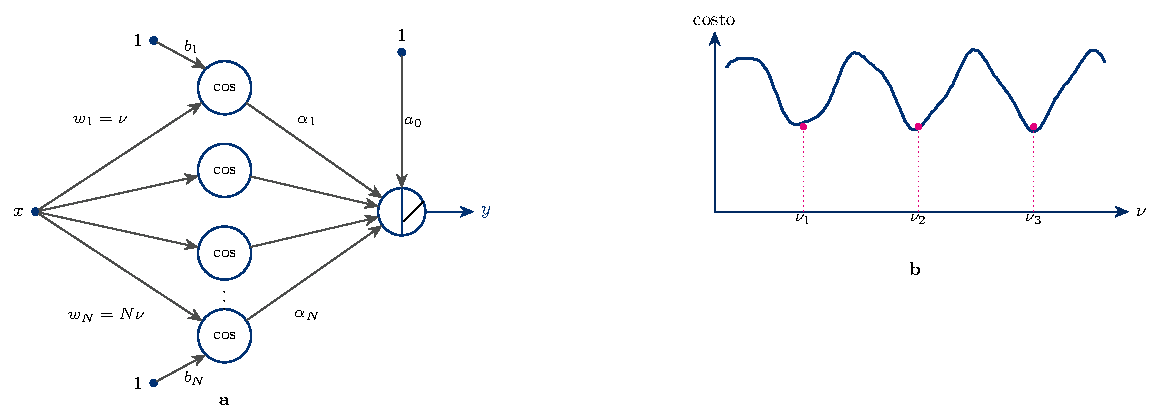
\includegraphics[max width=\linewidth]{Fig29.pdf}
\caption{{\bf a.} Red neuronal con una capa escondida y función de activación $\cos(x)$. {\bf b.} La función costo alcanza sus mínimos locales para ciertos valores del hiperparámetro $\nu$.}
\label{fig29}
\end{figure}

Afirmamos que esta red puede aproximar uniformemente cualquier función continua y periódica. En efecto, consideremos $f\colon \R\to\R$ una función continua y periódica con período $T$. Es decir $f(x+T)=f(x)$. Sea $\nu=\frac{2\pi}{T}$ la frecuencia asociada. Consideremos ahora pesos de la forma $w_j = j\nu$. Aplicando fórmulas trigonométricas elementales, tenemos
\begin{align*}
y &= a_0 + \sum_{j=1}^N \alpha_j \cos(j\nu x + b_j)\\
&=a_0 + \sum_{j=1}^N \alpha_j \cos(j\nu x)\cos(b_j) - \alpha_j \sin(j\nu x)\sin(b_j)\\
&=a_0 + \sum_{j=1}^N a_j \cos(j\nu x) - c_j \sin(j\nu x),
\end{align*}
con coeficientes $a_j = \alpha_j \cos(b_j)$ y $c_j = \alpha_j\sin(b_j)$. Por el Ejercicio \ref{ej.7.11.7}, los polinomios trigonométricos son densos en el conjunto de funciones periódicas sobre $\R$ con período $T$. Luego, dado $\ve>0$ existen $N\ge1$ y $a_0,\alpha_j, b_j\in \R$ (a partir de $a_j,c_j$ se recuperan $\alpha_j=\sqrt{a_j^2+c_j^2}$ y $b_j$ por coordenadas polares) tales que
$$
\left| a_0 + \sum_{j=1}^N \alpha_j \cos(j\nu x + b_j) - f(x)\right| < \ve. 
$$
Observemos que la frecuencia $\nu=\frac{2\pi}{T}$ viene dada por la función objetivo y que los pesos de entrada de la capa oculta son sus múltiplos enteros $j\nu$.

Es posible modificar este método, de manera heurística, para buscar frecuencias escondidas en una señal continua. Consideremos la señal objetivo $z=f(x)$ donde $x$ denota el tiempo. El peso $\nu$ del cálculo anterior se toma como un hiperparámetro. Luego, para cada valor de $\nu$ fijo se ajustan los otros parámetros, por ejemplo, usando el método de descenso de gradiente. Después se varía el valor de $\nu$ y se obtienen diferentes valores de la función de costo. Elegimos aquellos valores de $\nu$ para los que la función de costo alcanza mínimos locales, ver Figura \ref{fig29} {\bf b}. Esperamos que estos mínimos se correspondan con frecuencias propias contenidas en la señal. Esto es una heurística y no un teorema: el costo, como función de $\nu$, es muy poco regular y depende de $N$, del intervalo de observación y del método de optimización. Además, si $f$ tiene período $T$, también tiene período $mT$, y la red con frecuencia $\nu/m$ (con $N$ suficientemente grande) contiene a la de frecuencia $\nu$; por lo tanto aparecerán también mínimos en los submúltiplos $\nu/m$, y la frecuencia fundamental debe interpretarse como la {\em mayor} de las frecuencias en las que el costo es pequeño.

\section{Teoremas Tauberianos de Wiener}\label{sec.c7.4}

Para poder enunciar los teoremas Tauberianos es necesario introducir a la {\em Transformada de Fourier}.

Recordemos que $f\in L^1(\R)$ si se verifica que
$$
\int_{-\infty}^\infty |f(x)|\, dx < \infty,
$$
Tenemos entonces la siguiente definición
\begin{defi}[Transformada de Fourier]\label{def.fourier}
Dada $f\in L^1(\R)$ se define su transformada de Fourier, notada por $\F[f]$ o por $\hat f$ a
$$
\F[f](\xi) = \hat f(\xi) = \int_{-\infty}^\infty f(x) e^{-i x\xi}\, dx.
$$
\end{defi}
Es fácil ver que si $f\in L^1(\R)$ entonces $\hat f$ está bien definida y resulta una función acotada,
$$
|\hat f(\xi)|\le \int_{-\infty}^\infty |f(x)|\, dx,\quad \forall \xi\in\R.
$$
Algunos ejemplos:
\begin{enumerate}
\item \label{DE}{\em Doble exponencial.} Sea $f(x)=e^{-\lambda|x|}$, con $\lambda>0$. Entonces
$$
\hat f(\xi) = \frac{2\lambda}{\lambda^2 + \xi^2}.
$$

\item \label{LP} {\em Potencial de Laplace.} Sea $f(x) = \frac{1}{a^2+x^2}$, con $a>0$. Entonces
$$
\hat f(\xi) = \frac{\pi}{a} e^{-a|\xi|}.
$$

\item \label{G} {\em Gaussiana.} Sea $f(x) = e^{-ax^2}$, con $a>0$. Entonces
$$
\hat f(\xi) = \sqrt{\frac{\pi}{a}} e^{-\frac{\xi^2}{4a}}.
$$
\end{enumerate}

\subsection{Aprendiendo señales en $L^1(\R)$}
Tenemos el siguiente teorema que fue probado por N. Wiener en \cite{Wiener}
\begin{teo}\label{teo.wiener1}
Sea $f\in L^1(\R)$ y consideremos las traslaciones $f_\tau(x) = f(x+\tau)$ con $\tau\in\R$. Entonces el subespacio generado por la familia $\{f_\tau\colon \tau\in\R\}$ es denso en $L^1(\R)$ si y sólo si $\hat f(\xi)\neq 0$ para todo $\xi\in\R$.
\end{teo}

Observemos que los ejemplos \ref{DE}, \ref{LP}, \ref{G} verifican las hipótesis del Teorema \ref{teo.wiener1}.

La manera en la que se usa este resultado es la siguiente. Consideremos una red neuronal con función de activación $f\in L^1(\R)$ que verifica $\hat f(\xi)\neq 0$. Luego, por el Teorema \ref{teo.wiener1}, para toda $g\in L^1(\R)$ y $\ve>0$, tenemos una función 
$$
G(x) = \sum_{j=1}^N \alpha_j f(x+\tau_j),\qquad \alpha_j, \tau_j\in\R,\ N=1,2,\dots,
$$
tal que 
$$
\|g-G\|_1 = \int_\R |g(x)-G(x)|\, dx <\ve.
$$
La función $G(x)$ es la salida de una red neuronal con una capa oculta con función de activación $f$, pesos de salida $\alpha_j$ y sesgos $\tau_j$; los pesos de entrada son todos iguales a $1$, es decir, la red sólo traslada la activación $f$ y no la dilata. La aproximación es en norma $L^1$ y no punto a punto.

\subsection{Aprendiendo señales en $L^2(\R)$}
Recordemos que una función $f$ pertenece a $L^2(\R)$ si
$$
\int_{-\infty}^\infty |f(x)|^2\, dx < \infty,
$$

En general, una función $f$ puede pertenecer a $L^2(\R)$ pero no a $L^1(\R)$ y viceversa. Si $f$ pertenece a $L^2(\R)$ pero no a $L^1(\R)$ la expresión para la transformada de Fourier de $f$ no puede ser dada por la fórmula de la Definición \ref{def.fourier}. Sin embargo, es posible extender la definición de la transformada de Fourier al espacio $L^2(\R)$ de manera tal que si $f\in L^2(\R)\cap L^1(\R)$ entonces ambas definiciones coincidan. Ver, por ejemplo, \cite{Bonder}.

En \cite{Wiener} se demuestra el siguiente resultado, análogo al Teorema \ref{teo.wiener1}, para funciones de $L^2(\R)$.
\begin{teo}\label{teo.wiener2}
Sea $f\in L^2(\R)$ y consideremos las funciones trasladadas $f_\tau(x)= f(x+\tau)$ para $\tau\in\R$. Entonces el subespacio generado por la familia $\{f_\tau\colon \tau\in\R\}$ es denso en $L^2(\R)$ si y sólo si $\hat f(\xi)\neq 0$ para casi todo $\xi\in\R$.
\end{teo}

Observemos que los ejemplos \ref{DE}, \ref{LP}, \ref{G} también verifican las hipótesis del Teorema \ref{teo.wiener2}.

El Teorema \ref{teo.wiener2} se utiliza de manera similar al Teorema \ref{teo.wiener1}. Consideremos una red neuronal con función de activación $f\in L^2(\R)$ que verifica $\hat f(\xi)\neq 0$ en casi todo punto. Luego, por el Teorema \ref{teo.wiener2}, para toda $g\in L^2(\R)$ y $\ve>0$, tenemos una función 
$$
G(x) = \sum_{j=1}^N \alpha_j f(x+\tau_j),\qquad \alpha_j, \tau_j\in\R,\ N=1,2,\dots,
$$
tal que 
$$
\|g-G\|_2^2 = \int_\R |g(x)-G(x)|^2\, dx <\ve.
$$
La función $G(x)$ es la salida de una red neuronal con una capa oculta con función de activación $f$, pesos $\alpha_j$ y sesgos $\tau_j$.


\begin{obs}
Obviamente, la aplicación de los Teoremas \ref{teo.wiener1} y \ref{teo.wiener2} tiene limitaciones. Por ejemplo las funciones que vimos en los ejemplos \ref{DE}, \ref{LP}, \ref{G} son de forma {\em campana}, mientras que las funciones de activación más usadas son de tipo sigmoide o de tipo {\em palo de hockey} (función logística, ReLU, etc.) y no pertenecen a $L^1(\R)$ o a $L^2(\R)$.
\end{obs}

\section{Principio de contracción}\label{sec.c7.5}
En esta sección veremos aplicaciones del principio de contracción (Teorema de punto fijo de Banach) a redes neuronales.

Repasemos el principio de contracción. Si $(X, d)$ es un espacio métrico, una función $A\colon X\to X$ se dice una contracción si existe $\lambda\in (0,1)$ tal que
$$
d(A(x), A(y))\le \lambda d(x, y),\qquad \forall x, y\in X.
$$
Observemos que toda contracción resulta ser uniformemente continua.

\begin{ejem}
Si consideramos $X=\R$, entonces toda función $A\colon \R\to\R$ diferenciable con $|A'(x)|\le\lambda<1$ es una contracción. En efecto, por el Teorema de valor medio,
$$
|A(x)-A(y)| = |A'(\xi)(x-y)|\le \lambda |x-y|.
$$
Un ejemplo de función $A$ que verifica estas hipótesis es $A(x) = \frac12\cos(x)$.
\end{ejem}

El teorema de punto fijo de Banach dice lo siguiente.
\begin{teo}[Banach]\label{teo.punto.fijo}
Sean $(X, d)$ un espacio métrico completo y $A\colon X\to X$ una contracción. Entonces $A$ posee un único punto fijo. Es decir, existe un único punto $x_0\in X$ tal que $A(x_0) = x_0$.
\end{teo}

Este teorema se demuestra habitualmente en los cursos de Cálculo Avanzado y de Análisis Avanzado.


La salida de una red neuronal con una capa oculta teniendo función de activación $\varphi$ es dada por
\begin{equation}\label{formulaA}
A(x) = \sum_{j=1}^N \alpha_j \varphi(w_j x + b_j),
\end{equation}
donde asumimos que las entradas y salidas son números reales, es decir $A\colon\R\to\R$.

Tenemos entonces la siguiente proposición.
\begin{prop}\label{A.contraccion}
Sea $A(x)$ dada por la expresión \eqref{formulaA} y asumamos que la función $\varphi\colon \R\to\R$ verifica que $|\varphi'(x)|\le M$ para todo $x\in\R$. Entonces $A(x)$ es una contracción si se verifica
\begin{equation}\label{cotaM}
\sum_{j=1}^N (\alpha_j^2 + w_j^2) < \frac{2}{M}.
\end{equation}
\end{prop}

\begin{proof}
Observemos primero que
$$
|\varphi(x)-\varphi(y)|=|\varphi'(\xi)||x-y|\le M|x-y|,\qquad \forall x, y\in\R.
$$
Ahora,
\begin{align*}
|A(x)-A(y)| &= \left|\sum_{j=1}^N \alpha_j (\varphi(w_j x + b_j) - \varphi(w_j y + b_j))\right|\\
&\le \sum_{j=1}^N |\alpha_j| |\varphi(w_j x + b_j) - \varphi(w_j y + b_j)|\\
&\le M|x-y|\sum_{j=1}^N |\alpha_j||w_j|\\
&\le  \frac{M}{2}\left(\sum_{j=1}^N \alpha_j^2 + w_j^2 \right) |x-y|.
\end{align*}
Luego, si llamamos
$$
\lambda = \frac{M}{2}\left(\sum_{j=1}^N \alpha_j^2 + w_j^2 \right),
$$
tenemos, por \eqref{cotaM}, que $0<\lambda<1$ como queríamos ver.
\end{proof}

\begin{obs}
En el caso en que tomemos como función de activación a la función logística $\sigma(x) = (1+e^{-x})^{-1}$, tenemos que $0<\sigma'(x)\le \frac14$, de donde obtenemos que $A(x)$ es una contracción si se verifica que
$$
\sum_{j=1}^N (\alpha_j^2 + w_j^2) < 8.
$$
\end{obs}

\begin{cor}
Sea $A(x)$ dada por \eqref{formulaA} tal que la función de activación $\varphi$ verifica $|\varphi'(x)|\le M$ para todo $x\in\R$. Asumamos que los coeficientes $\alpha_j$ y $w_j$ verifican \eqref{cotaM}. Entonces existe un único $x_0\in \R$ tal que $A(x_0)=x_0$.
\end{cor}

\subsection{Aplicaciones a redes neuronales recurrentes}
En esta sección, una {\em unidad neuronal} significará una red neuronal con una capa escondida para las que se verifica la condición \eqref{cotaM} de la Proposición \ref{A.contraccion}, teniendo un ingreso $x\in\R$ y una salida $A(x)\in\R$ dada por la fórmula \eqref{formulaA}. Una unidad neuronal se muestra en la figura \ref{fig30}

\begin{figure}[htbp]
\centering
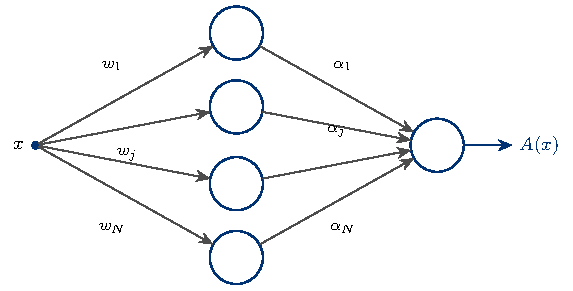
\includegraphics[max width=\linewidth]{Fig30.pdf}
\caption{Una unidad neuronal de tres capas cuya salida es una contracción.}
\label{fig30}
\end{figure}

Ahora, concatenamos varias unidades neuronales para construir una {\em red neuronal recurrente} como se muestra en la Figura \ref{fig31}. Esto significa que la salida de la $n-$ésima unidad neuronal es la entrada de la $(n+1)$ unidad neuronal, para $n\ge 1$. La salida de la $n-$ésima unidad es $A^n(x) = (A\circ\cdots\circ A)(x)$. En un primer momento, supongamos que los pesos y sesgos de todas las unidades neuronales son los mismos y el aprendizaje de la red no está supervisado, es decir que no hay una función objetivo específica. 

La pregunta es: {\em ¿Qué aprende este tipo de red?}

\begin{figure}[htbp]
\centering
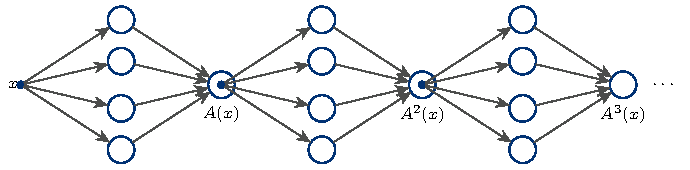
\includegraphics[max width=\linewidth]{Fig31.pdf}
\caption{Una red neuronal recurrente construida a partir de unidades neuronales de tres capas.}
\label{fig31}
\end{figure}

Para ser más precisos, asumamos que para cada valor de entrada $x\in\R$, la $n-$ésima salida, $y_n = A^n(x)$ es una sucesión convergente con límite $y$, que depende obviamente de $x$. Si definimos $y=\Lambda(x)$, entonces la función aprendida por la red es $\Lambda(x)$.

El siguiente resultado trata sobre existencia, unicidad y la forma de esta función.
\begin{prop}\label{prop.pto,fijo}
Sea $A$ una contracción. En la red neuronal recurrente construida en la Figura \ref{fig31}, para toda entrada $x\in\R$ la sucesión de salidas $y_n=A^n(x)$ converge a $x_0$, el único punto fijo del mapa $y=A(x)$. Es decir, $\Lambda(x)\equiv x_0$: la red ``aprende'' la función constante $x_0$.
\end{prop}

\begin{proof}
La demostración de este resultado es muy similar a la demostración del Teorema de Banach, Teorema \ref{teo.punto.fijo}.

En efecto, para cada valor de entrada $x$, consideramos la sucesión de números reales $y_n=A^n(x)$. Debemos probar que $\{y_n\}_{n\in\N}$ es convergente, pero para eso veamos que es una sucesión de Cauchy.

Usando la propiedad de contracción de la función $A(x)$, estimamos la diferencia entre dos elementos consecutivos de la sucesión
\begin{align*}
|y_{n+1}-y_n| &= |A^{n+1}(x) - A^{n}(x)| = |A(A^n(x)) - A(A^{n-1}(x))|\\
&\le \lambda |A^n(x)-A^{n-1}(x)| = \lambda |y_n-y_{n-1}|.
\end{align*}
Iterando esta desigualdad, llegamos a
$$
|y_{n+1}-y_n|\le \lambda^n |y_1-x|.
$$
Sea ahora $m=n+k$ y estimamos la diferencia entre dos términos arbitrarios de la sucesión usando la desigualdad triangular, y recordando que $\lambda\in (0,1)$,
\begin{equation}\label{7.8.3}
\begin{split}
|y_{n+k}-y_n| &\le \sum_{j=0}^{k-1} |y_{n+j+1}-y_{n+j}|  \le \sum_{j=0}^{k-1} \lambda^{n+j}|y_1-x|\\
&\le \lambda^n |y_1-x|\sum_{j=0}^\infty \lambda^j = \frac{\lambda^n}{1-\lambda} |y_1-x|,
\end{split}
\end{equation}
lo que prueba que $\{y_n\}_{n\in\N}$ es de Cauchy, por lo que existe $y\in\R$ tal que $y_n\to y$ cuando $n\to \infty$. Notemos $y=\Lambda(x)$. 

Veamos ahora que $y$ es el único punto fijo de $A(x)$ con lo que se concluye la demostración. Pero tenemos que
$$
|A(y)-y|\le |A(y)-y_n| + |y_n-y| = |A(y)-A(y_{n-1})| + |y_n-y|.
$$
Al ser $A$ una contracción, resulta continua. Luego tomando límite $n\to\infty$ en la última desigualdad, obtenemos que $|A(y)-y|=0$, con lo que $A(y)=y$, es decir, $y$ es un punto fijo de $A$. La unicidad es una consecuencia directa de la contracción, ya que si $y$ e $y'$ son dos puntos fijos, entonces
$$
|y-y'| = |A(y)-A(y')|\le \lambda |y-y'|,
$$
y como $\lambda\in (0,1)$ sigue que $|y-y'|=0$, o lo que es lo mismo que $y=y'$.
\end{proof}

\begin{obs}
Es sencillo estimar el error cometido al aproximar el punto fijo $x_0$ de $A$ por la sucesión aproximante $y_n$. Tomando límite $k\to\infty$ en la cota \eqref{7.8.3}, obtenemos
$$
|y_n-x_0|\le \frac{\lambda^n}{1-\lambda} |A(x)-x|.
$$
El valor de $n\in\N$, que es la profundidad de la red, puede ser elegido de manera tal que el error sea tan pequeño como queramos.
\end{obs}

Si cambiamos los pesos de la red, esto lleva al aprendizaje de diferentes constantes. Veamos que estas constantes dependen continuamente de los pesos. Empecemos con el concepto de proximidad de redes.
\begin{defi}
Dos redes neuronales se dicen $\ve-$cercanas en $I\subset (-R, R)\subset \R$ si para algún $\ve>0$ sus mapas de salida verifican
$$
|A(x) - \bar A(x)|<\ve, \qquad \forall x\in I\subset \R.
$$
\end{defi}

En otras palabras, dos redes son próximas si sus mapas de salida están próximos con respecto a la distancia de supremo.

\begin{lema}\label{7.8.4}
Consideremos dos unidades neuronales con mapas de salida dados por 
$$
A(x) = \sum_{j=1}^N \alpha_j \varphi(w_j x+ b_j) \quad \text{y}\quad \bar A(x) = \sum_{j=1}^N \bar\alpha_j \varphi(\bar w_j x+ \bar b_j),
$$
donde la función de activación $\varphi$ verifica $|\varphi(x)|\le C$ y $|\varphi'(x)|\le M$ para todo $x\in \R$.

Entonces, si
$$
\sum_{j=1}^N \left(M|\alpha_j|(R |w_j-\bar w_j| + |b_j-\bar b_j|) + C|\alpha_j-\bar\alpha_j|\right) <\ve,
$$
entonces las unidades neuronales están $\ve-$cercanas en $I$.
\end{lema}

\begin{proof}
Observemos primero que
\begin{align*}
|\alpha_j \varphi(w_j x + b_j) - \bar\alpha_j \varphi(\bar w_j x + \bar b_j)| \le& |\alpha_j| |\varphi(w_j x + b_j) - \varphi(\bar w_j x + \bar b_j)|\\
& +|\alpha_j -\bar \alpha_j| |\varphi(\bar w_j x + \bar b_j)| \\
\le &|\alpha_j| |\varphi'(\xi)| (|w_j-\bar w_j| |x| + |b_j-\bar b_j|)\\
&+ C|\alpha_j - \bar\alpha_j|\\
\le & |\alpha_j| M(|w_j-\bar w_j| |x| + |b_j-\bar b_j|) +  C|\alpha_j - \bar\alpha_j|
\end{align*}
Luego, 
\begin{align*}
|A(x)-\bar A(x)|&\le \sum_{j=1}^N|\alpha_j \varphi(w_j x + b_j) - \bar\alpha_j \varphi(\bar w_j x + \bar b_j)|\\
&\le \sum_{j=1}^N|\alpha_j| M(|w_j-\bar w_j| |x| + |b_j-\bar b_j|) +  C|\alpha_j - \bar\alpha_j|<\ve,
\end{align*}
como queríamos probar.
\end{proof}

\begin{obs}
De la demostración es evidente de que en el caso $I=\R$, entonces se debe pedir que $w_j=\bar w_j$,  $b_j=\bar b_j$ y
$$
\sum_{j=1}^N |\alpha_j - \bar\alpha_j| < \frac{\ve}{C}.
$$
\end{obs}

\begin{lema}
Consideremos dos unidades neuronales $\ve-$cercanas en $I$ con mapas de entrada-salida dados por $A(x)$ y $\bar A(x)$ respectivamente. Notemos por $x_0$ y $\bar x_0$ los respectivos puntos fijos y supongamos que $\bar x_0\in I$ (esto es automático si $I=\R$). Entonces $|x_0-\bar x_0|<\frac{1}{1-\lambda}\ve$, donde $\lambda\in (0,1)$ es el factor de contracción de $A$.
\end{lema}

\begin{proof}
Sea $\bar x_0$ el punto fijo del mapa $\bar A$ y sea $\lambda\in (0,1)$ el factor de contracción de $A$. Si llamamos $y_n = A^n(\bar x_0)$, entonces por la Proposición \ref{prop.pto,fijo}, tenemos que $y_n\to x_0$ donde $x_0$ es el punto fijo de $A$. Por otro lado, si en la desigualdad \eqref{7.8.3} tomamos $n=0$ (y $x=\bar x_0$, de modo que $y_0=\bar x_0$), obtenemos que
$$
|y_k - \bar x_0| \le \frac{1}{1-\lambda} |A(\bar x_0) - \bar x_0|.
$$
Tomando límite cuando $k\to\infty$, obtenemos
$$
|x_0-\bar x_0|\le \frac{1}{1-\lambda} |A(\bar x_0) - \bar x_0|.
$$
Por otro lado,
$$
 |A(\bar x_0) - \bar x_0| =  |A(\bar x_0) - \bar A(\bar x_0)|<\ve,
$$
donde usamos que $\bar x_0\in I$. Esto concluye la demostración.
\end{proof}

Tenemos entonces el siguiente corolario inmediato.
\begin{cor}
Consideremos dos unidades neuronales como en el Lema \ref{7.8.4}, con los mismos $w_j$ y $b_j$ (y distintos $\alpha_j,\bar\alpha_j$) y ambas contracciones, y sea $\lambda$ el factor de contracción de $A$. Entonces, dado $\ve>0$, tomando $\delta=(1-\lambda)\ve/C$ se tiene
$$
\sum_{j=1}^N |\alpha_j - \bar \alpha_j|<\delta \Longrightarrow |x_0-\bar x_0|<\ve,
$$
donde $x_0$ y $\bar x_0$ son los puntos fijos de los mapas de entrada-salida de las unidades neuronales. En efecto, por la observación anterior las unidades son $(1-\lambda)\ve$-cercanas en $I=\R$ y se aplica el lema.
\end{cor}

\subsection{Redes resonantes}
Consideramos una red neuronal con dos capas, ver Figura \ref{fig32}. La información se transmite de un lado a otro entre las capas hasta que eventualmente converge a un estado estacionario.  

\begin{figure}[htbp]
\centering
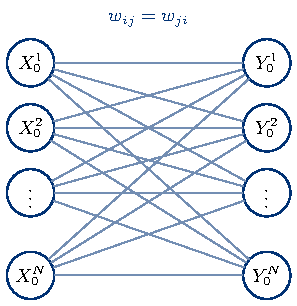
\includegraphics[max width=\linewidth]{Fig32.pdf}
\caption{Una red neuronal resonante.}
\label{fig32}
\end{figure}


Sea $N$ el número de neuronas en cada capa. El estado inicial de la capa de la izquierda está dado por el vector $X_0$. Esto induce el estado en la segunda capa  
$$
Y_0 = \varphi(WX_0 + b),
$$
donde los pesos se asumen simétricos, es decir, $w_{ij} = w_{ji}$.

Esta información se retroalimenta a la primera capa, lo que proporciona la salida  
$$
X_1 = \varphi(WY_0 + b).
$$
Aquí, $\varphi$ es la función de activación para ambas capas y $b$ es el vector de sesgo común.

De esta manera, obtenemos las sucesiones $\{X_n\}_{n\in\N}$ y $\{Y_n\}_{n\in\N}$ definidas recursivamente por el sistema  
$$
Y_n = \varphi(WX_n + b),\quad X_n = \varphi(WY_{n-1} + b), \quad n \geq 1.
$$
Esto puede reformularse en términos de dos recurrencias como  
$$
Y_n = F(Y_{n-1}),\quad X_n = F(X_{n-1}),
$$
donde $F\colon \R^N\to \R^N$ está dada por  
$$
F(U) = \varphi \left( W \varphi(WU + b) + b \right).
$$
El estado estacionario de la red corresponde al par de puntos fijos $(X^*, Y^*)$, donde  
$$
F(X^*) = X^*, \quad F(Y^*) = Y^*.
$$

Abordaremos este problema utilizando el Principio de Contracción, Teorema \ref{teo.punto.fijo}. Primero, reescribimos el problema de manera equivalente de la siguiente forma. Definimos  
$$
Z_0 = X_0, \quad Z_1 = Y_0, \quad Z_2 = X_1,
$$
y en general,  
$$
Z_{n+1} = G(Z_n),
$$
donde  
$$
G(Z) = \varphi(WZ + b).
$$

Basta con demostrar que $\{Z_n\}_{n\in\N}$ es una sucesión de vectores que converge a algún vector $Z^*$. Como $G\colon \R^N \to \R^N$ y $\varphi$ actúa componente a componente, se tiene $|\varphi(u_i)-\varphi(v_i)|\le\|\varphi'\|_\infty|u_i-v_i|$ y, por lo tanto,
$$
\|G(Z') - G(Z)\|_2 \leq \|\varphi'\|_{\infty}\, \|W(Z' - Z)\|_2 \leq \|\varphi'\|_{\infty} \|W\| \|Z' - Z\|_2, \quad \forall Z, Z' \in \R^N,
$$
donde $\|W\|$ es la norma de operador (espectral) de $W$. (Equivalentemente, el jacobiano es $DG(Z)=\operatorname{diag}(\varphi'(WZ+b))\,W$.)

Si los pesos satisfacen la desigualdad  
$$
\|W\| < \frac{1}{\|\varphi'\|_{\infty}},
$$
entonces $G$ se convierte en una aplicación contractiva. El Teorema \ref{teo.punto.fijo} garantiza que $G$ tiene un único punto fijo $Z^*$, al cual converge la sucesión $\{Z_n\}_{n\in\N}$. En particular $X_n=Z_{2n}\to Z^*$ e $Y_n=Z_{2n+1}\to Z^*$, de modo que $X^*=Y^*=Z^*$. (La simetría $w_{ij}=w_{ji}$ expresa que las dos capas se conectan con la misma matriz: de la primera a la segunda con $W$ y de vuelta con $W^t=W$; no se usa en la estimación.)

La conclusión es que si los pesos $w_{ij}$ son suficientemente pequeños, el estado de la red tiende a un {\em estado estable} o {\em estado resonante}.


\section{Resumen}\label{sec.c7.6}
Este capítulo contiene algunos resultados clásicos de análisis real útiles para la representación de redes neuronales.

Para el aprendizaje de funciones continuas $f \in C([a, b])$, se requiere la convergencia uniforme. Si la red genera una sucesión de funciones continuas que converge puntualmente a la función objetivo $f$ y el error $|f-f_n|$ decrece con $n$, podemos concluir que la convergencia es uniforme con el Teorema de Dini, Teorema \ref{teoDini}.

Otra técnica para construir una sucesión de funciones uniformemente convergente en un conjunto compacto es mediante el Teorema de Arzela-Ascoli. En este caso, se puede extraer una subsucesión convergente de un conjunto de funciones que es uniformemente acotado y equicontinuo. Como consecuencia, el conjunto de salidas de las redes de una capa oculta, con función de activación sigmoide y pesos acotados, es relativamente compacto en $C([a,b])$: toda sucesión de tales redes tiene una subsucesión que converge uniformemente a alguna función continua (que no se conoce a priori y no es necesariamente una función objetivo dada).

Otro método de aproximación de funciones continuas en un conjunto compacto es mediante el Teorema de Stone-Weierstrass. Este resultado también puede utilizarse para ver que las redes con activación coseno aproximan uniformemente las funciones continuas periódicas.

Las funciones objetivo en los espacios $L^1$ y $L^2$ pueden ser aproximadas (en las respectivas normas) por traslaciones de una activación fija utilizando los teoremas tauberianos de Wiener. Estos teoremas se aplican principalmente a funciones de activación con forma de campana.

El principio de contracción, el cual garantiza la existencia de un punto fijo, puede aplicarse a las funciones de mapeo entrada-salida de una red neuronal de una capa oculta, así como a redes resonantes. Mediante la iteración del mapeo entrada-salida, se obtiene que la red recurrente converge a una constante (el punto fijo), que depende continuamente de los pesos.


\section{Ejercicios}\label{sec.c7.7}

\begin{ejer}
Sea $\F=\{\tanh(ax+b)\colon a, b\in\R\}$. Mostrar que la familia $\F$ es uniformemente acotada.
\end{ejer}

\begin{ejer}
Sea $\F=\{ax+b\colon |a|+|b|<1,\ x\in [0, 1]\}$. Mostrar que la familia es equicontinua y uniformemente acotada.
\end{ejer}

\begin{ejer}
Sea $M>0$ y consideremos la familia
$$
\F = \left\{f\in C^1([a, b])\colon \int_a^b |f'(x)|^2\, dx \le M\right\}.
$$
Mostrar que $\F$ es equicontinua.
\end{ejer}

\begin{ejer}
Notemos por $\D\subset (a, b)$ un conjunto denso. Sea $\F$ la familia de funciones tales que
\begin{itemize}
\item[(a)] Es equicontinua sobre el intervalo $(a, b)$.
\item[(b)] Para todo $x\in \D$, la familia es uniformemente acotada en $x$, es decir, existe $M>0$ tal que $|f(x)|\le M$ para toda $f\in\F$. 
\end{itemize}
Mostrar que $\F$ es uniformemente acotada en todos los puntos.
\end{ejer}

\begin{ejer}
Sean $\F$ una familia equicontinua, $k\ge 1$ un entero fijo y $\{w_1,\dots,w_k\}$ un conjunto de pesos tales que $|w_j|<1$ para $j=1,\dots,k$. Mostrar que el conjunto sigue siendo equicontinuo si se extiende para incluir a las combinaciones lineales de la forma $\sum_{j=1}^k w_j f_j$ con $f_j\in\F$, $j=1,\dots,k$.
\end{ejer}

\begin{ejer}
Una red neuronal usando neuronas sigmoides es diseñada para aprender una función continua $f\in C([a, b])$ por el método de descenso de gradiente. La salida de la red obtenida luego de la $n-$ésima actualización de los parámetros es denotada por $G_n(x) = G(x; w(n), b(n))$. Asumamos que en cada paso la aproximación no empeora, es decir $|f(x)-G_{n+1}(x)| \le |f(x) - G_n(x)|$ para todo $x\in [a, b]$ y todo $n\ge 1$, y que $G_n(x)\to f(x)$ para cada $x\in[a,b]$. Probar (por ejemplo, con el Teorema de Dini) que $G_n$ converge uniformemente a $f$ en $[a, b]$. Mostrar con un ejemplo que, sin la hipótesis de convergencia puntual, la conclusión es falsa (tomar $f=0$ y $G_n=\frac12+2^{-n}$).
\end{ejer}

\begin{ejer}\label{ej.7.11.7}
Sea $f\colon\R\to\R$ una función continua y periódica con período $T>0$, i.e. $f(x+T)=f(x)$ para todo $x\in\R$. Mostrar que para todo $\ve>0$, existe una función
$$
F(x) = a_0 + \sum_{n=1}^N \left(a_n\cos\frac{2\pi nx}{T} + b_n \sin\frac{2\pi nx}{T}\right),
$$
tal que $|F(x)-f(x)|<\ve$ para todo $x\in \R$.
\end{ejer}

\begin{ejer}[El conjunto de transformaciones integrales de funciones $L^2$]\label{ej.7.11.10}
Sea $M>0$ y sea $K\colon [a, b]\times [c, d]\to \R$ una función continua. Se define la clase
$$
\F_M = \left\{ g(x) = \int_c^d K(x, y)h(y)\, dy\colon h\in C([c, d]),\ \int_c^d |h(y)|^2\, dy \le M\right\}.
$$
Mostrar que $\F_M$ es equicontinuo y uniformemente acotado.
\end{ejer}

\begin{ejer}
Se define la clase
$$
\A = \left\{\sum_{i=1}^n \alpha_i e^{m_i x}\colon \alpha_i\in\R,\ m_i\in\N_0,\ n=1,2,\dots\right\}.
$$
Mostrar que $\A\subset C([a, b])$ es un álgebra de funciones. Probar que dada $f\in C([a, b])$ y $\ve>0$, existen $\alpha_1,\dots,\alpha_n\in\R$ y $m_1,\dots,m_n\in\N_0$ tales que
$$
\left| f(x) - \sum_{i=1}^n \alpha_i e^{m_i x}\right| < \ve,\quad \forall x\in [a, b].
$$
Formular una interpretación en términos de aprendizaje automático de este resultado.
\end{ejer}

%%%%%%%%%%%%%%%%%%%%%%%%%%%%%%%%%%%%%%%%
%% CAPITULO 8 %%%%%%%%%%%%%%%%%%%%%%%%%%%%%%%
%%%%%%%%%%%%%%%%%%%%%%%%%%%%%%%%%%%%%%%%

\chapter{Aprendizaje con entradas unidimensionales}\label{cap8}

Este capitulo analiza el caso de una red neuronal cuya entrada es acotada y unidimensional, por ejemplo, $x\in[0, 1]$. Aparte de su simplicidad, este caso es importante desde una serie de puntos de vista: puede ser tratado de manera elemental sin hacer uso del arsenal de herramientas del análisis funcional (como lo haremos en el Capítulo \ref{cap9}) y, por la naturaleza constructiva de este caso, provee un algoritmo explícito para hallar los pesos de la red.

Los casos de redes neuronales con una capa oculta y neuronas de tipo perceptron y sigmoides serán estudiados. Adicionalmente estudiaremos con detalle el aprendizaje usando ReLU y Softplus.

Se estudia el aprendizaje de funciones de una variable. Después de unos resultados preliminares (Sección~\ref{sec.c8.1}), se muestra cómo aproximar con una red de perceptrones (Sección~\ref{sec.c8.2}), con una red sigmoide (Sección~\ref{sec.c8.3}), con neuronas ReLU (Sección~\ref{sec.c8.4}) y con Softplus (Sección~\ref{sec.c8.5}), todas con una capa escondida. Corresponde al Capítulo~8 de~\cite{Calin}.

\section{Resultados preliminares}\label{sec.c8.1}

En esta sección usaremos las nociones de derivadas generalizadas, medida, integración y medida de Dirac. A no asustarse que introduciremos esos conceptos de manera simple y accesible.

\begin{enumerate}
\item Veamos primero que toda función simple (función escalón), puede escribirse como una combinación lineal de traslaciones de la función de Heaviside.

Suponiendo que la función simple tiene soporte en el intervalo $[0, 1]$, la misma puede escribirse como
$$
c(x) = \sum_{i=1}^N \alpha_i \I_{[x_{i-1}, x_i)}(x),
$$
donde $0=x_0<x_1<\cdots<x_N=1$ es una partición del intervalo $[0, 1]$ y $\I_{[x_{i-1}, x_i)}(x)$ es la función indicadora del intervalo $[x_{i-1}, x_i)$.

Observemos que la indicadora $\I_{[x_{i-1}, x_i)}(x)$ se puede escribir como diferencia de dos funciones de Heaviside trasladadas,
$$
\I_{[x_{i-1}, x_i)}(x) = H(x-x_{i-1}) - H(x-x_i).
$$
Luego obtenemos fácilmente que
\begin{equation}\label{8.1.1}
c(x) = \sum_{i=1}^N \alpha_i \I_{[x_{i-1}, x_i)}(x) = \sum_{i=0}^N c_i H(x-x_i),
\end{equation}
donde $c_0=\alpha_1$, $c_i=\alpha_{i+1}-\alpha_i$ para $1\le i\le N-1$ y $c_N=-\alpha_N$. (En $[0,1)$ el último término es nulo, pues $H(x-x_N)=0$ para $x<1$.)

\item Una consecuencia del ítem anterior es que la derivada de una función simple es una combinación lineal de deltas de Dirac,
$$
c'(x) = \frac{d}{dx} \sum_{i=0}^N c_i H(x-x_i) =  \sum_{i=0}^N c_i \delta(x-x_i) =  \sum_{i=0}^N c_i \delta_{x_i}(x).
$$
Esta relación se interpreta como que la sensibilidad de la salida con respecto a la entrada, $c'(x)$ es la superposición de $N+1$ golpes ($\delta_{x_i}$) de magnitud $c_i$.

\item La delta de Dirac se puede aproximar (débilmente) por medidas de probabilidad con densidades de forma de campana. Más precisamente, tenemos
\begin{prop}\label{prop.ve.delta}
Consideremos una función de activación $\varphi\colon\R\to\R$ que satisface:
\begin{itemize}
\item[(i)] $\varphi$ es creciente (no decreciente);
\item[(ii)] $\varphi(\infty) - \varphi(-\infty)=1$ (en particular existen ambos límites y son finitos);
\item[(iii)] $\varphi$ es de clase $C^1$.
\end{itemize}
Para $\ve>0$ definimos $\varphi_\ve(x) = \varphi(\frac{x}{\ve})$ y consideremos la medida de probabilidad $\mu_\ve$ con densidad dada por $\varphi_\ve'(x)$. Entonces $\mu_\ve\to\delta$ cuando $\ve\downarrow 0$ en sentido débil, es decir, $\int g\,d\mu_\ve\to g(0)$ para toda $g$ continua y acotada.
\end{prop}
\begin{proof}
Por (i)--(iii), $\varphi'\ge0$ y $\int_\R\varphi'=\varphi(\infty)-\varphi(-\infty)=1$, de modo que $\varphi'$ es una densidad de probabilidad y $\mu_\ve$ es, en efecto, una medida de probabilidad (ver más abajo). Sea $g$ continua y acotada. Tenemos
$$
\int_{-\infty}^\infty \varphi_\ve'(x) g(x)\, dx = \int_{-\infty}^\infty \frac{1}{\ve}\varphi'(\tfrac{x}{\ve}) g(x)\, dx = \int_{-\infty}^\infty \varphi'(y) g(\ve y)\, dy.
$$
Como $g(\ve y)\to g(0)$ para cada $y$ (por continuidad) y $|\varphi'(y)g(\ve y)|\le \|g\|_\infty\varphi'(y)$, con $\varphi'$ integrable, el teorema de convergencia dominada permite tomar límite cuando $\ve\downarrow 0$:
$$
\lim_{\ve\downarrow 0} \int_{-\infty}^\infty \varphi'(y) g(\ve y)\, dy = g(0) \int_{-\infty}^\infty \varphi'(y)\, dy = g(0)(\varphi(\infty) - \varphi(-\infty)) = g(0).
$$
Luego
$$
\lim_{\ve\downarrow 0}\int_{-\infty}^\infty  g(x)\, d\mu_\ve(x) = \lim_{\ve\downarrow 0}\int_{-\infty}^\infty \varphi_\ve'(x) g(x)\, dx  = g(0) = \int_{-\infty}^\infty g(x)\, d\delta(x). 
$$
Como $g$ es una función continua y acotada arbitraria, obtenemos que $\mu_\ve\to\delta$ cuando $\ve\downarrow 0$ en sentido débil.
\end{proof}

Un ejemplo de función $\varphi$ que satisface las hipótesis de la Proposición \ref{prop.ve.delta} es la función logística
$$
\varphi(x) = \frac{1}{1+e^{-x}}.
$$
Observemos que tanto $\varphi'$ como $\varphi_\ve'$ tienen forma de {\em campana} (un pulso positivo de área $1$), y que el pico se hace más alto y más angosto a medida que $\ve\downarrow 0$; el {\em salto} es $\varphi$, cuya derivada es el pulso.

Observemos también que 
$$
\int_\R d\mu_\ve = \int_\R \varphi'_\ve(x)\, dx = \int_\R\frac{1}{\ve}\varphi'(\tfrac{x}{\ve}) \, dx = \int_\R \varphi'(y)\, dy = 1,
$$
lo que implica que $\mu_\ve$ es una medida de probabilidad para todo $\ve>0$.

\item La convolución de una función $f(x)$ con la delta de Dirac centrada en un punto $x_0$, $\delta_{x_0}(x) = \delta(x-x_0)$, coincide con la composición de $f$ con la traslación de tamaño $x_0$:
$$
(\delta_{x_0} * f)(x) = \int_\R \delta_{x_0}(y)f(x-y)\, dy = f(x-x_0).
$$
Esto puede enunciarse de manera equivalente diciendo que una señal $f(x)$ filtrada a través de la medida de Dirac $\delta_{x_0}$ da la misma señal a la que se le aplicó un cambio de fase.

\item Un resultado importante que se estudia tanto en Cálculo Avanzado como en Análisis Avanzado es que toda función continua definida en un intervalo compacto $g\colon [a, b]\to\R$ resulta ser {\em uniformemente continua}.
\end{enumerate}

\section{Red de perceptrones con una capa escondida}\label{sec.c8.2}

Consideremos una red neuronal con una capa escondida, funciones de activación en la capa escondida dada por la función de Heaviside y una función de activación lineal en la capa de salida. Vamos a mostrar que esta red puede aproximar uniformemente cualquier función continua $g\in C([0, 1])$. Equivalentemente, cualquier función continua definida en un intervalo compacto puede ser aproximada uniformemente por funciones simples. La red está representada en la Figura \ref{fig33}.

\begin{figure}[htbp]
\centering
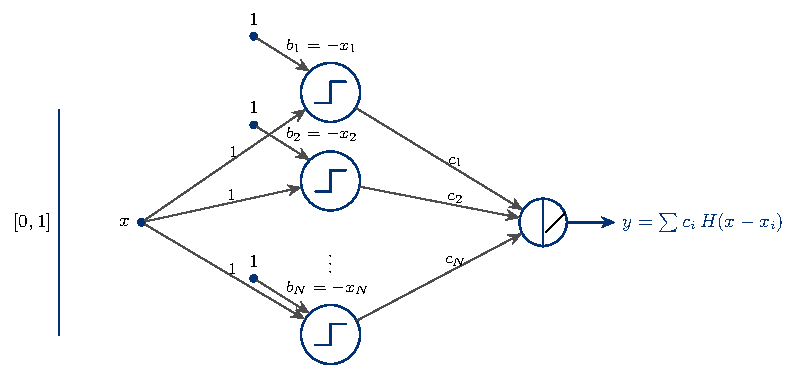
\includegraphics[max width=\linewidth]{Fig33.pdf}
\caption{Una red neuronal con una capa oculta compuesta por perceptrones con pesos iguales a 1 y pesos de salida igual a $c_i$ y sesgos $-x_i$ (la neurona $i$ se activa cuando $x\ge x_i$).}
\label{fig33}
\end{figure}

Notemos primero que el lado derecho de la ecuación \eqref{8.1.1} es una salida particular de esta red. El siguiente resultado muestra que la red aproxima funciones continuas por funciones escalón.
\begin{prop}\label{prop.aprox.perceptron}
Sea $g\in C([0,1])$. Entonces, para todo $\ve>0$, existe una función simple $s(x) = \sum_{i=0}^{N-1} c_i H(x-x_i)$ tal que
$$
|g(x)-s(x)|< \ve,\quad \forall x\in [0, 1].
$$
\end{prop}

\begin{proof}
Sea $\ve>0$ y sea $\delta>0$ el asociado a la continuidad uniforme de $g(x)$ en el intervalo $[0, 1]$. Tomemos $N\in\N$ tal que $\frac{1}{N}<\delta$ y consideremos la partición uniforme del intervalo $[0, 1]$, $x_i = \frac{i}{N}$, $i=0, 1,\dots, N$. Observemos que, por la continuidad uniforme, tenemos que
$$
|g(x)-g(x_i)|<\ve,\quad \forall x\in [x_i, x_{i+1}).
$$
Definimos inductivamente los números $c_i$, $i=0, 1, \dots, N-1$ de la forma
\begin{align*}
g(x_0) &= c_0\\
g(x_1) &= c_0+c_1\\
&\vdots\\
g(x_{N-1})&= c_0+c_1+\cdots+c_{N-1}.
\end{align*}
Observemos también que si $x\in [x_i, x_{i+1})$, entonces
$$
H(x-x_j) = \begin{cases}
1, & \text{si } j\le i\\
0, & \text{si } j>i.
\end{cases}
$$
Luego, si definimos la función simple $s(x)$ como
$$
s(x) = \sum_{i=0}^{N-1} c_i H(x-x_i),
$$
tenemos que $s(x) = g(x_i)$ si $x\in [x_i, x_{i+1})$, $i=0,\dots,N-1$, y $s(1)=g(x_{N-1})$.

En conclusión, obtenemos que
$$
|g(x)-s(x)| = |g(x)-g(x_i)| < \ve, \quad \text{si } x\in [x_i, x_{i+1}),\ i=0,1,\dots,N-1,
$$
y también $|g(1)-s(1)|=|g(1)-g(x_{N-1})|<\ve$, pues $1-x_{N-1}=\frac1N<\delta$. Esto concluye la demostración.
\end{proof}

\begin{obs}\label{obs.perceptron}
Observemos que en la demostración del resultado anterior los pesos $c_i$ vienen dados por
$$
c_0=g(0),\qquad c_i = g(x_i)-g(x_{i-1}),\quad i=1,\dots,N-1,
$$
y dado que $x_i-x_{i-1} = \frac{1}{N} < \delta$ obtenemos que $|c_i|<\ve$ para $i\ge1$. El primer peso $c_0=g(0)$ no es pequeño en general: corresponde a la neurona $H(x-x_0)=H(x)$, que vale $1$ en todo $[0,1]$ y juega el papel de un sesgo de salida.

Notemos finalmente que para poder tener pesos de la capa de salida pequeños, el precio que se paga es que $N$ (el número de neuronas) sea grande.
\end{obs}

\section{Red sigmoide con una capa escondida}\label{sec.c8.3}

Consideremos una red neuronal con una capa escondida con función de activación logística o cualquier función de tipo sigmoide, que notamos por $\varphi$, para la capa oculta y función de activación lineal para la capa de salida. Asumimos que $\varphi$ verifica las hipótesis de la Proposición \ref{prop.ve.delta} (la logística las verifica; $\tanh$ también, tras normalizar $\frac{1+\tanh}{2}$). Veremos que esta red es capaz de aproximar uniformemente cualquier función continua $g\in C([0, 1])$.

El resultado principal de esta sección es el siguiente.
\begin{teo}\label{teo.aprox.sigmoide}
Consideremos una función de activación $\varphi$ que verifica las hipótesis de la Proposición \ref{prop.ve.delta} y sea $g\in C([0, 1])$. Entonces, dado $\ve>0$, existen $N\ge 1$ y $c_i, w, b_i,\beta \in\R$ tales que
$$
\left| g(x) - \beta - \sum_{i=1}^N c_i\varphi(wx + b_i)\right| < \ve,\quad \forall x\in [0, 1].
$$
\end{teo}

El sesgo de salida $\beta$ es necesario en general (por ejemplo, si $g$ es constante no nula y $\varphi(-\infty)=0$ hace falta una neurona saturada o un sesgo). Si $\varphi(\infty)\neq0$, puede absorberse aproximadamente con una neurona adicional $\varphi(wx+b_0)$ con $b_0$ grande, que vale $\approx\varphi(\infty)$ en todo $[0,1]$ (para $w>0$).

\begin{proof}
La idea general de la demostración es la siguiente. Como primer paso, usamos la Proposición \ref{prop.aprox.perceptron} para obtener una función simple que aproxime $g(x)$. Luego, usamos un proceso de {\em regularización por convolución} para aproximar la función de Heaviside por versiones suaves de la misma y veremos que esas regularizaciones se pueden escribir como combinaciones lineales de nuestra función sigmoide $\varphi$. Sea $L=\varphi(-\infty)$, de modo que $\varphi(\infty)=L+1$.

\subsubsection*{{\em Paso 1:}  Aproximación de $g$ por una función simple.}

Aplicamos la demostración de la Proposición \ref{prop.aprox.perceptron} y la Observación \ref{obs.perceptron} con $\ve/4$ en lugar de $\ve$, y con $N\ge2$: obtenemos $x_i=i/N$ y una función simple
$$
s(x)=\sum_{i=0}^{N-1}c_iH(x-x_i)=g(0)+c(x),\qquad c(x)=\sum_{i=1}^{N-1}c_iH(x-x_i),
$$
(recordemos que $H(x-x_0)=H(x)=1$ en $[0,1]$) con
$$
|g(x)-s(x)|<\frac{\ve}{4},\quad \forall x\in [0, 1],\qquad |c_i|<\frac{\ve}{4}\ \ (i=1,\dots,N-1).
$$

\subsubsection*{{\em Paso 2:} Regularización de la función escalonada $c$.}

Para $\alpha>0$ sea $\psi_\alpha(x) = \frac{1}{\alpha}\varphi'(\frac{x}{\alpha})$ (el {\em pulso} asociado a $\varphi_\alpha(x)=\varphi(\frac{x}{\alpha})$, $\psi_\alpha=\varphi_\alpha'$). Por la Proposición \ref{prop.ve.delta}, $\psi_\alpha$ es la densidad de una medida de probabilidad $\mu_\alpha$ que converge débilmente a $\delta$ cuando $\alpha\downarrow 0$. Definimos la función regularizada de $c$ por
$$
c_\alpha(x) = (c * \psi_\alpha)(x) = \int_\R c(y)\psi_\alpha(x-y)\, dy = \int_\R \psi_\alpha(y)\,c(x-y)\,dy.
$$
Calculamos $c_\alpha$ usando que $H(t-y)=1$ si y sólo si $y\le t$:
$$
(H(\cdot-x_i)*\psi_\alpha)(x)=\int_{-\infty}^{x-x_i}\psi_\alpha(y)\,dy=\varphi\!\left(\frac{x-x_i}{\alpha}\right)-L .
$$
Por lo tanto
$$
c_\alpha(x)=\sum_{i=1}^{N-1}c_i\left[\varphi\!\left(\frac{x-x_i}{\alpha}\right)-L\right]
=\sum_{i=1}^{N-1}c_i\,\varphi(wx+b_i)-L\sum_{i=1}^{N-1}c_i,
$$
con $w=\frac1\alpha$ y $b_i=-\frac{x_i}{\alpha}$. Es decir, $c_\alpha$ es la salida de una red con una capa oculta sigmoide, salvo una constante (que absorbe el sesgo de salida). Esto es lo que se llama {\em regularización por convolución}: la salida de la red de Heaviside es filtrada por el pulso $\psi_\alpha$.

\subsubsection*{{\em Paso 3:} Aproximación de la función escalonada por la regularizada.}
Vamos a mostrar que 
$$
|c(x) - c_\alpha(x)| < \frac{\ve}{2},\quad \forall x\in \R,
$$
si $\alpha$ es suficientemente chico. Como $\psi_\alpha$ es una densidad de probabilidad, escribimos
$$
c(x)-c_\alpha(x) = \int_\R \psi_\alpha(y) (c(x)-c(x-y))\, dy.
$$
Sea $\delta=\frac1N$ y dividamos la integral en la región $|y|<\delta$ y su complemento,
$$
c(x)-c_\alpha(x) = \underbrace{\int_{\{|y|<\delta\}}\psi_\alpha(y) (c(x)-c(x-y))\, dy}_{I(\alpha)} + \underbrace{\int_{\{|y|\ge\delta\}}\psi_\alpha(y) (c(x)-c(x-y))\, dy}_{II(\alpha)}.
$$
Para $I(\alpha)$: si $|y|<\delta$, el intervalo de extremos $x-y$ y $x$ tiene longitud menor que la separación $\frac1N$ entre los saltos, de modo que contiene a lo sumo un punto $x_i$; luego $c(x)-c(x-y)$ es $0$ o $\pm c_j$ para algún $j$, y $|c(x)-c(x-y)|<\frac\ve4$. Entonces $|I(\alpha)|\le\frac\ve4\int\psi_\alpha=\frac{\ve}4$.

Para $II(\alpha)$: $c$ es acotada, $|c(x)|\le M:=\sum_{i=1}^{N-1}|c_i|$, de donde $|c(x)-c(x-y)|\le 2M$. Haciendo el cambio de variables $y=\alpha z$,
$$
\int_{\{|y|\ge\delta\}}\psi_\alpha(y)\,dy=\int_{\{|z|\ge\delta/\alpha\}}\varphi'(z)\,dz\longrightarrow0\quad(\alpha\downarrow0),
$$
pues $\varphi'$ es integrable. Luego $|II(\alpha)|\le 2M\int_{\{|y|\ge\delta\}}\psi_\alpha<\frac\ve4$ si $\alpha$ es chico. Sumando, $|c(x)-c_\alpha(x)|<\frac\ve2$ para todo $x\in\R$.

\subsubsection*{{\em Paso 4:} Conclusión.}

Fijado $\alpha$ como en el Paso 3, definimos $\beta=g(0)-L\sum_{i=1}^{N-1}c_i$. Por el Paso 2,
$$
\beta+\sum_{i=1}^{N-1}c_i\varphi(wx+b_i)=g(0)+c_\alpha(x).
$$
Entonces, para $x\in[0,1]$,
$$
\left|g(x)-\beta-\sum_{i=1}^{N-1}c_i\varphi(wx+b_i)\right|=|g(x)-g(0)-c_\alpha(x)|\le |g(x)-s(x)|+|c(x)-c_\alpha(x)|<\frac\ve4+\frac\ve2<\ve,
$$
lo que concluye la demostración (con $N-1$ neuronas ocultas).
\end{proof}

\begin{obs}
\begin{itemize}
\item[(i)] Observemos que en el caso unidimensional, el peso $w$ no depende de la neurona $i$.
\item[(ii)] La salida de la red con función de activación sigmoide (salvo la constante $-L\sum c_i$),
$$
y = \sum_{i=1}^N c_i\varphi(w x + b_i),
$$
se obtuvo {\em filtrando} la salida de la red con función de activación Heaviside
$$
y = \sum_{i=1}^N c_i H(x - x_i),
$$
a través del filtro $\varphi'_\alpha(x)$.

\item[(iii)] Los resultados de estas dos últimas secciones muestran que cualquier función continua en un intervalo compacto, puede ser aproximada de dos maneras: la Proposición \ref{prop.aprox.perceptron} asegura que puede ser aproximada por funciones simples, mientras que el Teorema \ref{teo.aprox.sigmoide} asegura que se puede aproximar por funciones suaves. Sin embargo el resultado del Teorema \ref{teo.aprox.sigmoide} es más útil, dado que el aproximante es suave, lo que hace posible el uso del algoritmo de retropropagación.
\end{itemize}
\end{obs}

\section{Aprendizaje con funciones ReLU}\label{sec.c8.4}

Recordemos que la función ReLU (Rectified Linear Unit) se define como
$$
ReLU(x) = xH(x) = \begin{cases}
x, &\text{si } x\ge 0\\
0, &\text{si } x<0,
\end{cases}
$$
y observemos que $ReLU'(x) = (xH(x))' = H(x) + xH'(x) = H(x) + x\delta(x) = H(x)$.

Veremos en lo que sigue que la función de salida de una red neuronal con una capa oculta, función de activación ReLU en la capa oculta y función lineal de activación en la capa de salida produce funciones que son lineales a trozos, así que nuestro primer resultado será mostrar que esta clase de funciones (las lineales a trozos) son densas en el conjunto de las funciones continuas.

\begin{lema}\label{lema.lineal.trozos}
Sea $g\in C([a, b])$. Entonces, dado $\ve>0$ existe una partición $a=x_0<x_1<\cdots<x_N=b$ de manera tal que la función $h(x)$ que pasa por los puntos $(x_i, g(x_i))$, $i=0,\dots,N$ y es lineal en cada intervalo $I_i= [x_{i-1}, x_i]$, $i=1,\dots,N$, verifica
$$
|g(x)-h(x)|<\ve,\quad \forall x\in [a, b].
$$
\end{lema}

\begin{proof}
Dado $\ve>0$, como $g$ es uniformemente continua en $[a, b]$, existe $\delta>0$ tal que
$$
|g(x)-g(y)|<\frac{\ve}{2} \quad \forall x, y\in [a, b], \text{ tal que }  |x-y|<\delta.
$$
Tomemos $N\ge 1$ tal que $\frac{b-a}{N}<\delta$ y definimos la partición uniforme como $x_i = a+i\frac{b-a}{N}$, $i=0,\dots, N$.

La función lineal a trozos asociada a $g$ y a la partición $\{x_i\}_{i=0}^N$ queda entonces definida como
$$
h(x) = g(x_{i-1}) + m_i(x-x_{i-1}), \quad \text{si } x\in I_i = [x_{i-1}, x_i],
$$
donde la pendiente $m_i$ se define por
$$
m_i = \frac{g(x_i)-g(x_{i-1})}{x_i - x_{i-1}}.
$$
Como $h$ es lineal en $I_i$, tenemos que
$$
|h(x_i) - h(x)|\le |h(x_i)-h(x_{i-1})| = |g(x_i)-g(x_{i-1})| < \frac{\ve}{2},\quad \forall x\in I_i.
$$
Luego, si $x\in [a, b]$, entonces existe $i=1,\dots,N$ tal que $x\in I_i$ y tenemos
\begin{align*}
|g(x)-h(x)| & \le |g(x)-g(x_i)| + |g(x_i)-h(x)|\\
& \le |g(x)-g(x_i)| + |h(x_i) - h(x)|\\
& < \frac{\ve}{2} + \frac{\ve}{2} = \ve.
\end{align*}
Esto concluye la demostración.
\end{proof}

Con la ayuda de este lema, podemos demostrar que una red neuronal con una capa oculta que usa ReLU como función de activación para la capa oculta y una función lineal como función de activación para la capa de salida puede aproximar uniformemente cualquier función continua.
\begin{teo}\label{teo.ReLU}
Consideremos una red neuronal con una capa oculta con ReLU como función de activación para esta capa oculta y función de activación lineal y sesgo $\beta$ para la capa de salida, Sea $g\in C([a, b])$ dada. Entonces, dado $\ve>0$, existen $\alpha_j, b_j\in \R$ y $N\ge 1$ tales que
$$
\left| g(x) - \sum_{j=0}^{N-1} \alpha_j ReLU(x+b_j) - \beta\right| < \ve,\quad \forall x\in [a, b].
$$
\end{teo}

\begin{proof}
La demostración consiste en ver que la función de salida de esta red,
\begin{equation}\label{salidaReLU}
y= G(x) = \sum_{j=0}^{N-1} \alpha_j ReLU(x+b_j) + \beta,
\end{equation}
puede representar a cualquier función lineal a trozos como, por ejemplo, las consideradas en el Lema \ref{lema.lineal.trozos}.

Para eso, tomemos $N$ y la partición uniforme $x_j=a+j\Delta$, $\Delta=\frac{b-a}{N}$, $j=0,\dots,N$, dadas por el Lema \ref{lema.lineal.trozos}, y sea $h$ la función lineal a trozos asociada a $g$ y a esa partición. Vamos a mostrar que podemos elegir los parámetros $\alpha_j$ y $\beta$ de manera tal que la función dada por \eqref{salidaReLU}, con sesgos $b_j=-x_j$, coincida con $h$.

Notemos que
$$
ReLU(x_k-x_j) = \begin{cases}
0,& \text{si } k\le j\\
(k-j)\Delta,& \text{si } k>j,
\end{cases}
$$
luego, la función $G(x)$ dada por \eqref{salidaReLU} evaluada en los puntos de la partición $x_k$ toma los valores
$$
G(x_k) = \sum_{j=0}^{N-1} \alpha_j ReLU(x_k-x_j) + \beta = \Delta \sum_{j<k} \alpha_j (k-j) + \beta.
$$
Si llamamos $y_k=g(x_k)$, queremos $G(x_k)=y_k$, $k=0,\dots,N$, es decir, el sistema (triangular, de $N+1$ ecuaciones con $N+1$ incógnitas $\beta,\alpha_0,\dots,\alpha_{N-1}$)
$$\begin{cases}
y_0=G(x_0)= \beta\\
y_1 = G(x_1) = \Delta\,\alpha_0 + \beta\\
y_2 = G(x_2) = \Delta\,(2\alpha_0 + \alpha_1) + \beta\\
\cdots \\
y_N = G(x_N) = \Delta\,\big(N\alpha_0 + (N-1)\alpha_1+\cdots + \alpha_{N-1}\big) + \beta.
\end{cases}
$$
Este sistema tiene una única solución dada por
$$
\begin{cases}
\beta = y_0\\
\alpha_0 = \dfrac{y_1-y_0}{\Delta}\\[1ex]
\alpha_j = \dfrac{y_{j+1}-2y_j+y_{j-1}}{\Delta},\quad j=1,\dots,N-1,
\end{cases}
$$
es decir, $\alpha_0$ es la primera pendiente y $\alpha_j=m_{j+1}-m_j$ es el cambio de pendiente en $x_j$ (una diferencia segunda). Finalmente, $G$ es continua, lineal en cada intervalo $[x_j,x_{j+1}]$ (pues $G'(x)=\sum_{j}\alpha_jH(x-x_j)$ es constante allí) y coincide con $g$ en los puntos $x_k$; por lo tanto $G=h$, y el resultado se sigue del Lema \ref{lema.lineal.trozos}.
\end{proof}

\section{Aprendizaje con Softplus}\label{sec.c8.5}
La función de activación {\em softplus} se define como
$$
\varphi(x) = sp(x) = \ln(1+e^x).
$$
Es una versión suave de la función $ReLU(x)$. Esto se puede formalizar en una proposición.
\begin{prop}\label{K.conv}
La función softplus, se puede escribir como
$$
sp(x) = (ReLU * K)(x) = \int_{-\infty}^\infty ReLU(y) K(x-y)\, dy,
$$
donde el {\em núcleo de convolución} $K$ viene dado por
$$
K(x) = \frac{1}{(1+e^x)(1+e^{-x})}.
$$
\end{prop}

\begin{proof}
Observemos primero que $K(x)$ es una función positiva que decrece a 0 exponencialmente rápido cuando $x\to\pm \infty$. Esta propiedad hace que la convolución y las integrales impropias que siguen estén todas bien definidas. Ahora, observemos que el núcleo $K$ es la derivada de la función logística $\sigma(x) = (1+e^{-x})^{-1}$, i.e. $K(x) = \sigma'(x)$. Por otro lado, $sp(x)$ es la primitiva de $\sigma(x)$, es decir $sp'(x) = \sigma(x)$, luego,
$$
sp(x) = \int_{-\infty}^x \sigma(t)\, dt.
$$
Con estas observaciones, ya podemos calcular el producto de convolución:
\begin{align*}
(ReLU(x)* K)(x) &= \int_{-\infty}^\infty ReLU(y) K(x-y)\, dy = \int_0^\infty y K(x-y)\, dy\\
&= \int_{-\infty}^x (x-t)K(t)\, dt = x\int_{-\infty}^x K(t)\, dt - \int_{-\infty}^x tK(t)\, dt\\
&= x\sigma(x) - \int_{-\infty}^x t\sigma'(t)\, dt\\
&=x\sigma(x) - \left(t\sigma(t)\Big|_{-\infty}^x - \int_{-\infty}^x \sigma(t)\, dt\right)\\
&=x\sigma(x) - \left(x\sigma(x) - sp(x)\right) = sp(x),
\end{align*}
lo que prueba el resultado.
\end{proof}

\begin{obs}
Una prueba alternativa y {\em formal} de esta proposición, puede hacerse usando las relaciones
$$
ReLU'(x) = H(x),\quad H'(x) = \delta(x),\quad sp'(x) = \sigma(x),\quad \sigma'(x) = K(x),
$$
y las fórmulas
$$
(f*g)'(x) = (f' * g)(x) = (f* g')(x).
$$
Efectivamente, si llamamos $f(x) = (ReLU * K)(x) - sp(x)$, entonces tenemos que $f(-\infty)=0$. Por otro lado,
\begin{align*}
f'(x) &= (ReLU * K)'(x) - sp'(x) = (ReLU' * K)(x) - \sigma(x)\\
&= (H * \sigma') (x) - \sigma(x) = (H'*\sigma)(x) - \sigma(x)\\
&=(\delta*\sigma)(x) - \sigma(x) = \sigma(x) - \sigma(x) = 0.
\end{align*}
Luego $f'\equiv0$ y, como $f(-\infty)=0$, resulta $f(x)=0$ para todo $x\in\R$.
\end{obs}

Veamos las propiedades del núcleo de convolución $K(x)$.
\begin{prop}\label{Kalpha}
El núcleo de convolución $K(x)$ definido en la Proposición \ref{K.conv} es una densidad de probabilidad simétrica en $\R$. 

Por otro lado, dado $\alpha>0$, consideramos los núcleos rescalados $K_\alpha(x) = \frac{1}{\alpha}K(\frac{x}{\alpha})$. Entonces $K_\alpha$ son densidades de probabilidad simétricas en $\R$ y las medidas de probabilidad $d\mu_\alpha = K_\alpha\, dx$ convergen a $\delta$ cuando $\alpha\downarrow 0$ en sentido débil.
\end{prop}

\begin{proof}
De la expresión $K(x) = (1+e^x)^{-1}(1+e^{-x})^{-1}$ es evidente que $K(x)=K(-x)$ y $K(x)>0$. Por otro lado,
$$
\int_{-\infty}^\infty K(x)\, dx = \int_{-\infty}^\infty \sigma'(x)\, dx = \sigma(\infty) - \sigma(-\infty) = 1.
$$
Ahora, usando la sustitución $x=\alpha y$ es fácil ver que 
$$
\int_{-\infty}^\infty K_\alpha(x)\, dx = \int_{-\infty}^\infty K(x)\, dx = 1.
$$
La demostración de que $d\mu_\alpha = K_\alpha\, dx \to d\delta$ cuando $\alpha\downarrow 0$ es análoga a la de la Proposición \ref{prop.ve.delta} (convergencia dominada, pues $K$ es integrable).
\end{proof}

Si ahora definimos las funciones softplus rescaladas
$$
\varphi_\alpha(x) = \alpha sp(\frac{x}{\alpha}) = \alpha\ln(1+e^{x/\alpha}),
$$
usando las relaciones $sp'(x)=\sigma(x)$ y $\sigma'(x) = K(x)$ obtenemos que
$$
\varphi''_\alpha(x) = K_\alpha(x).
$$
Es sencillo ver que las funciones rescaladas $\varphi_\alpha(x)$ convergen monótonamente a $ReLU(x)$ (ver Figura \ref{fig34})

\begin{figure}[htbp]
\centering
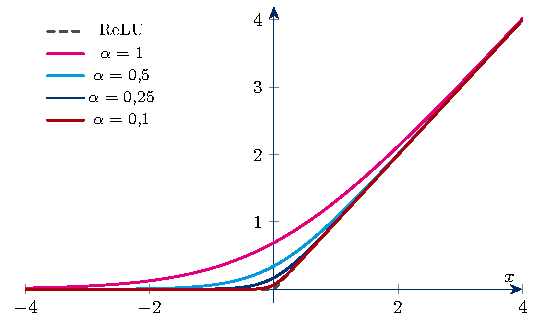
\includegraphics[max width=\linewidth]{Fig34.pdf}
\caption{Funciones softplus rescaladas $\varphi_\alpha(x)$ para diferentes valores de $\alpha$.}
\label{fig34}
\end{figure}

El siguiente resultado nos provee de una fórmula para la regularización de la función lineal a trozos $G(x)$ dada por el Teorema \ref{teo.ReLU} cuando la misma es pasada por el filtro $K_\alpha$.
\begin{lema}\label{Galpha}
Consideremos la convolución $G_\alpha(x) = (G * K_\alpha)(x)$, donde 
$$
G(x) = \sum_{j=0}^{N-1} \alpha_j ReLU(x-x_j) + \beta.
$$
Entonces, existen parámetros $c_j, w$ y $b_j$ tales que
$$
G_\alpha(x) = \sum_{j=0}^{N-1} c_j sp(wx+b_j)+\beta.
$$
\end{lema}

\begin{proof}
Primero calculamos $(ReLU*K_\alpha)$. Con el cambio de variables $y=\alpha z$ y la Proposición \ref{K.conv}, usando $ReLU(\alpha z)=\alpha ReLU(z)$,
$$
(ReLU*K_\alpha)(x)=\int_\R ReLU(y)\tfrac1\alpha K\!\left(\tfrac{x-y}{\alpha}\right)dy=\alpha\int_\R ReLU(z)K\!\left(\tfrac x\alpha-z\right)dz=\alpha\, sp\!\left(\tfrac x\alpha\right)=\varphi_\alpha(x).
$$
Como además $\int K_\alpha=1$ (la convolución con una constante la deja igual) y la convolución conmuta con traslaciones,
\begin{align*}
G_\alpha(x) &= \sum_{j=0}^{N-1}\alpha_j \big(ReLU(\cdot - x_j)*K_\alpha\big)(x) + \beta
= \sum_{j=0}^{N-1}\alpha_j \varphi_\alpha(x-x_j) + \beta\\
&=\sum_{j=0}^{N-1}\alpha_j\, \alpha\, sp\!\left(\frac{x-x_j}{\alpha}\right) + \beta = \sum_{j=0}^{N-1}c_j\,sp(wx+b_j) + \beta,
\end{align*}
donde $c_j = \alpha_j \alpha$, $w=1/\alpha$ y $b_j = -x_j/\alpha$. (Formalmente, esto es $ReLU''=\delta$ y $\varphi_\alpha''=K_\alpha$: $(ReLU*\varphi_\alpha'')=(ReLU''*\varphi_\alpha)=\delta*\varphi_\alpha$.)
\end{proof}

\begin{obs}
La función $G_\alpha$ es la salida de una red neuronal con una capa oculta con función de activación softplus para la misma y función de activación lineal para la capa de salida.
\end{obs}

Obtenemos entonces:
\begin{cor}\label{corGalpha}
La sucesión $G_\alpha$ definida en el Lema \ref{Galpha} converge uniformemente a $G$ cuando $\alpha\downarrow 0$.
\end{cor}

\begin{proof}
Por la fórmula del Lema \ref{Galpha} (con $\varphi_\alpha$) tenemos $G_\alpha(x)=\sum_j\alpha_j\varphi_\alpha(x-x_j)+\beta$. Como $0\le\varphi_\alpha(t)-ReLU(t)=\alpha\ln(1+e^{-|t|/\alpha})\le\alpha\ln2$ para todo $t\in\R$ (ver el Ejercicio \ref{ej8.8.6}), resulta
$$
|G_\alpha(x)-G(x)|\le \alpha\ln 2\sum_{j=0}^{N-1}|\alpha_j|\longrightarrow0\quad(\alpha\downarrow0),
$$
uniformemente en $x\in\R$. (Observemos que no se puede aplicar directamente el Teorema de Dini: los coeficientes $\alpha_j$ pueden tener signos distintos y entonces $G_\alpha$ no es monótona en $\alpha$.)
\end{proof}

Combinando ahora la Proposición \ref{Kalpha}, el Lema \ref{Galpha} y el Teorema \ref{teo.ReLU}, obtenemos el siguiente resultado:
\begin{teo}
Consideremos una red neuronal con una capa escondida con función de activación softplus y función de activación lineal en la capa de salida. Sea $g\in C([0,1])$. Entonces dado $\ve>0$, existen $N\ge 1$, $c_j,  w, b_j, \beta\in\R$, $j=0, \dots, N-1$, tales que
$$
\left| g(x) - \sum_{j=0}^{N-1} c_j sp(w x + b_j) - \beta\right| < \ve,\quad \forall x\in [0, 1].
$$
\end{teo}

\begin{proof}
Sea $\ve>0$. Por el Teorema \ref{teo.ReLU}, existe $G(x) = \sum_{j=0}^{N-1}\alpha_j ReLU(x-x_j)+\beta$ tal que
$$
|g(x)-G(x)| < \frac{\ve}{2}, \quad \forall x\in [0,1].
$$
El Corolario \ref{corGalpha} implica que existe $\alpha>0$ suficientemente chico tal que
$$
|G(x)-G_\alpha(x)|<\frac{\ve}{2},\quad \forall x\in [0,1].
$$
Luego, usando la desigualdad triangular junto con el Lema \ref{Galpha} se concluye lo pedido.
\end{proof}

\section{Resumen}\label{sec.c8.6}
Este capítulo muestra que las redes neuronales de una capa oculta con entrada unidimensional, $x\in [0,1]$, pueden aproximar uniformemente funciones continuas en $C([0, 1])$. Probamos este resultado en los casos en que la función de activación es una función escalón, una sigmoide, una ReLU o una función Softplus.

El resultado de una red con función de activación sigmoide es una versión suavizada de una red con función de activación escalón. De manera similar, el aprendizaje con Softplus es una versión suavizada del aprendizaje con ReLU. Los resultados de este capítulo son de existencia (densidad): no explican por qué, en la práctica, una activación suave suele entrenarse mejor que un escalón, ni cuándo conviene Softplus en lugar de ReLU. Para eso hay que considerar la optimización (por ejemplo, la derivada del escalón es nula salvo en un punto, de modo que no hay gradiente) y la generalización.

Una motivación práctica es que la construcción es explícita: dada una función continua (o sus valores en una grilla), se obtienen directamente los pesos de la red. Estos resultados, sin embargo, no dicen nada sobre la generalización a datos nuevos ni sobre el número de neuronas necesario en función de la regularidad de $g$.

\section{Ejercicios}\label{sec.c8.7}

\begin{ejer}[Derivada generalizada]
Decimos que $f^{(n)}=g$ en sentido generalizado (o sentido débil), si para toda función suave de soporte compacto $\phi\in C^\infty_c(\R)$ se tiene 
$$
(-1)^n \int_\R f(x)\phi^{(n)}(x)\, dx = \int_\R g(x)\phi(x)\, dx.
$$
Probar las siguientes relaciones en sentido generalizado:
\begin{itemize}
\item[(a)] $H'(x-x_0) = \delta(x-x_0)$;

\item[(b)] $ReLU'(x) = H(x)$;

\item[(c)] $ReLU''(x) = \delta(x)$;

\item[(d)] $(xReLU(x))' = 2ReLU(x)$;

\item[(e)] $(xReLU(x))'' = 2H(x)$.
\end{itemize}
\end{ejer}

\begin{ejer}[Continuidad uniforme]
Sea $g\colon [a, b]\to\R$ una función continua. Probar que es {\em uniformemente continua}.
\end{ejer}

\begin{ejer}
Sea $f$ una de las funciones de la Figura \ref{fig35}. ¿Cuál de ellas tiene la propiedad de que la familia
$$
\F = \left\{\sum_{i=1}^N \alpha_i f(w_i x - b_i)\colon N\ge 1,\ \alpha_i, w_i, b_i\in\R\right\}
$$
es densa en $C([0,1])$?
\end{ejer}

\begin{figure}[htbp]
\centering
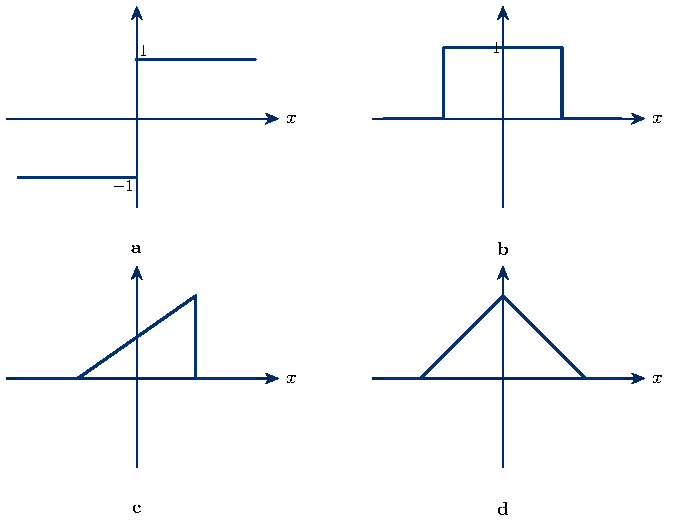
\includegraphics[max width=\linewidth]{Fig35.pdf}
\caption{{\bf a}. Función de salto bipolar. {\bf b}. Función cajón. {\bf c}. Función diente de sable. {\bf d}. Función diente de tiburón.}
\label{fig35}
\end{figure}

\begin{ejer}\label{ej8.8.6}
Sea $\varphi_\alpha(x) = \alpha \ln(1+e^{x/\alpha})$. Probar que $\varphi_\alpha(x)\downarrow ReLU(x)$ cuando $\alpha\downarrow 0$ y que $0\le\varphi_\alpha(x)-ReLU(x)\le\alpha\ln2$ para todo $x\in\R$.
\end{ejer}

%%%%%%%%%%%%%%%%%%%%%%%%%%%%%%%%%%%%%%%%
%% CAPITULO 9 %%%%%%%%%%%%%%%%%%%%%%%%%%%%%%%
%%%%%%%%%%%%%%%%%%%%%%%%%%%%%%%%%%%%%%%%

\chapter{Aproximadores universales}\label{cap9}

La respuesta a la pregunta “¿Por qué las redes neuronales funcionan tan bien en la práctica?” se basa, sin duda, en el hecho de que las redes neuronales pueden aproximar con gran precisión una amplia familia de funciones del mundo real que dependen de variables de entrada. El objetivo de este capítulo es proporcionar demostraciones matemáticas de este comportamiento para diferentes tipos de funciones objetivo.

El hecho de que las redes neuronales actúen como aproximadores universales significa que su salida es una aproximación precisa, con cualquier grado de exactitud deseado, de funciones en ciertos espacios de funciones bien conocidos. El proceso de obtener una aproximación precisa se interpreta como el aprendizaje de una función objetivo dada.

Este capítulo trata sobre la existencia del proceso de aprendizaje, pero no proporciona ninguna construcción explícita de los pesos de la red. La idea subyacente es que tiene sentido saber primero que una solución existe antes de comenzar a buscarla.

La solución deseada existe siempre que se considere un número suficiente de neuronas en la capa oculta y que la función objetivo pertenezca al espacio de funciones considerado (por ejemplo, que sea continua). Para obtenerla se debe emplear un algoritmo de aprendizaje adecuado. Que la solución exista no garantiza que un algoritmo de entrenamiento la encuentre, ni dice cuántas neuronas hacen falta: este capítulo es una justificación teórica de la {\em capacidad} de las redes, no del éxito de su uso en aplicaciones concretas.


Es el capítulo central de la parte analítica. Tras unos ejemplos (Sección~\ref{sec.c9.1}) y el planteo general (Sección~\ref{sec.c9.2}), se demuestra que las redes con una capa oculta son aproximadores universales (Sección~\ref{sec.c9.3}), y se aplica la idea al aprendizaje de soluciones de ecuaciones diferenciales (Sección~\ref{sec.c9.4}). Corresponde al Capítulo~9 de~\cite{Calin}.

\section{Ejemplos introductorios}\label{sec.c9.1}

Una red neuronal, como hemos visto, tiene la capacidad de aprender de los datos. Suponiendo que se tiene una función objetivo $z=f(x)$, la red tiene que aprender esta función cambiando sus parámetros internos. La mayoría de las veces, el resultado de este aprendizaje es sólo una aproximación aceptable. Veamos algunos ejemplos.

\begin{ejem}[Aprendiendo funciones continuas]
Supongamos que queremos armar una red neuronal para aprender la ley de gravitación universal de Newton. Esto es
$$
f(m_1, m_2, d) = \frac{k m_1 m_2}{d^2},
$$
es decir, la fuerza entre dos cuerpos de masas $m_1$ y $m_2$ es inversamente proporcional al cuadrado de la distancia entre ellos.

Construimos una red con entradas $(x_1, x_2, x_3) = (m_1, m_2, d)$ que puede tomar valores continuos en una cierta región compacta $K\subset \R^3$, por ejemplo $K=[m_{\min},m_{\max}]^2\times[d_{\min},d_{\max}]$ con $d_{\min}>0$ (la fuerza no es acotada cuando $d\to0$, así que hay que excluir $d=0$). La variable objetivo, que tiene que ser aprendida, es $z=f(m_1, m_2, d)$, con $f\colon K\to\R$ una función continua. La red tendrá salida $y=g(m_1, m_2, d, w, b)$, que depende tanto de las entradas como de los parámetros (pesos $w$ y sesgos $b$).

Luego, si uno provee las masas de dos cuerpos, junto con la distancia que los separa, la red debe ser capaz de proporcionar la fuerza entre ellos con una precisión mejor que el error de tolerancia prefijado. En el Teorema \ref{teo9.3.6} demostraremos la existencia de esta red.
\end{ejem}

\begin{ejem}[Aprendiendo funciones de energía finita]
Una señal de audio tiene que ser aprendida por una red neuronal. Es habitual en la teoría asumir que la señal es de {\em energía finita}, es decir que la señal pertenece al espacio $L^2$.

La entrada de la red es el tiempo $t\in[0,1]$ (normalizado) y la función objetivo $z=f(t)$ provee la amplitud de la señal en cada instante, con $f\in L^2([0,1])$. La salida de la red, $y=g(t, w, b)$ nos da una aproximación del objetivo que puede ser ajustada variando los pesos $w$ y los sesgos $b$. La existencia de una red neuronal con esta propiedad la veremos en el Corolario \ref{cor.U.denso.L2}.
\end{ejem}


\section{Planteo general}\label{sec.c9.2}

El concepto de red neuronal como aproximador universal es el siguiente. Sea $x$ la variable de entrada y $z$ la variable objetivo. La función objetivo es entonces $z=f(x)$ donde $f$ es una cierta función que pertenece a un espacio $E$ de funciones, un espacio métrico con distancia $d$, i.e. $f\in (E, d)$.

El conjunto de funciones que son salidas posibles de la red neuronal es un espacio que notamos por $U$ y se asume que $U\subset E$. De hecho, se elige la función de activación de la red de manera tal que la función de salida quede definida dentro del espacio $E$.

Luego, decimos que la red neuronal es un {\em aproximador universal} para el espacio $(E, d)$ si el conjunto de salida $U$ es denso en $E$, i.e.
$$
\forall f\in E,\ \forall \ve>0,\ \exists g\in U \text{ tal que } d(f, g)<\ve.
$$

El proceso por el que la red neuronal aproxima a la función objetivo $f\in E$ por funciones $g\in U$ se llama el aprendizaje y al conjunto $U$ se lo llama el espacio aproximante del espacio objetivo $E$.

Veamos algunos de los ejemplos más usuales de espacios objetivos $(E,  d)$.

\begin{ejem}[Espacio de funciones continuas]
El primer ejemplo es $E=C(K)$ donde $K\subset \R^n$ es un conjunto compacto. La distancia en este espacio es
$$
d(f, g) = \sup_{x\in K} |f(x)-g(x)|.
$$
Notemos que $(E, d)$ resulta un espacio métrico completo. De hecho, la métrica $d$ es inducida por una norma
$$
\|f\| = \sup_{x\in K} |f(x)|.
$$
Luego, $d(f, g) = \|f-g\|$.

Es habitual notar por $\|\cdot\|_\infty$ y $d_\infty(\cdot, \cdot)$ a esta norma y métrica respectivamente.
\end{ejem}

\begin{ejem}[Espacio de funciones integrables]
En este caso $E=L^1(K)$ es el espacio de funciones integrables sobre $K$ (con la medida de Lebesgue, identificando funciones que coinciden en casi todo punto). La métrica en este caso viene dada por
$$
d(f, g) = \int_K |f(x)-g(x)|\, dx.
$$
Esta métrica mide el área encerrada entre los gráficos de las funciones sobre $K$. Al igual que en el ejemplo anterior, esta métrica viene inducida por una norma
$$
\|f\| = \int_K |f(x)|\, dx.
$$
Esta norma y métrica se notan habitualmente como $\|\cdot\|_1$ y $d_1(\cdot,\cdot)$ respectivamente.
\end{ejem}

\begin{ejem}[Espacio de funciones de energía finita]
Este espacio es $E=L^2(K)$ y se define como
$$
L^2(K) = \left\{f\colon K\to\R\colon \int_K |f(x)|^2\, dx <\infty\right\}.
$$
La métrica viene dada por
$$
d(f, g) = d_2(f, g) = \left(\int_K |f(x)-g(x)|^2\, dx\right)^\frac12,
$$
es decir, la raíz cuadrada de la energía de la diferencia entre dos señales de energía finita $f$ y $g$ (sin la raíz no se verificaría la desigualdad triangular). Como en el ejemplo anterior, se identifican funciones que coinciden en casi todo punto. Al igual que en los ejemplos anteriores, esta métrica es inducida por una norma:
$$
\|f\| = \|f\|_2 = \left(\int_K |f(x)|^2\, dx \right)^\frac12.
$$
\end{ejem}

\begin{ejem}[Espacios discretos]
En este caso consideramos un conjunto finito de puntos $K=\{x_1,\dots,x_r\}\subset \R^n$ y consideramos el conjunto $E=\{f\colon K\to\R\}$ al conjunto de funciones reales definidas sobre $K$. En este conjunto se pueden definir diferentes métricas, por ejemplo
$$
d_s(f, g) = \left(\sum_{x_j\in K} |f(x_j)-g(x_j)|^2\right)^\frac12,
$$
que es la distancia Euclídea de puntos en $\R^n$, o
$$
d_a(f, g) = \sum_{x_j\in K} |f(x_j)-g(x_j)|,
$$
que es el error absoluto.
\end{ejem}

%\begin{ejem}[Convergencia en probabilidad]
%Sea $\mu$ una medida de probabilidad sobre $\R^n$ y definimos sobre el conjunto $E$ de funciones medibles Borel a la distancia
%$$
%d_\mu(f, g) = \inf\{\ve>0\colon \mu(\{ |f-g|>\ve\}) < \ve\},
%$$
%donde $\{|f-g|>\ve\} = \{x\in \R^n\colon |f(x)-g(x)|>\ve\}$.
%
%Veremos más adelante que convergencia en la métrica $d_\mu$ es equivalente a la convergencia en probabilidad.
%\end{ejem}

\section{Redes con una capa oculta}\label{sec.c9.3}

Comenzaremos el estudio del proceso de aprendizaje en el caso más simple en el que la red tiene una única capa oculta.

En esta sección mostraremos que una red neuronal con una capa oculta puede ser usada como un aproximador para los espacios $C(I_n)$, $L^1(I_n)$ y $L^2(I_n)$, donde $I_n = [0, 1]\times\cdots\times [0, 1] \subset \R^n$ es un hipercubo.


\subsection{Aprendiendo funciones continuas $f\in C(I_n)$}

Para poder desarrollar los resultados necesitaremos unos resultados preliminares de Análisis Funcional. Este resultado se lo conoce como el {\em lema de separación}.

\begin{lema}\label{lema.separacion}
Sea $E$ un espacio normado, $U\subset E$ un subespacio y $f_0\in E$ tal que
$$
d(f_0, U)\ge\delta,
$$
para algún $\delta>0$. Luego, existe un funcional $L\colon E\to\R$ lineal y continuo tal que
\begin{itemize}
\item[(a)] $\|L\|\le 1$ (i.e. $\sup_{\|f\|\le 1} |L(f)|\le 1$).

\item[(b)] $L(u)=0$ para todo $u\in U$.

\item[(c)] $L(f_0)=\delta$.
\end{itemize}
\end{lema}

Este lema es una consecuencia relativamente inmediata del Teorema de Hahn-Banach que se estudia en el curso de Análisis Funcional. Pueden encontrar una demostración del Teorema de Hahn-Banach, por ejemplo, en \cite{Brezis}.

El Teorema de Hahn-Banach dice:
\begin{teo}[Hahn-Banach]\label{HB}
Sea $E$ un espacio vectorial normado, con norma $\|\cdot\|$ y $U\subset E$ un subespacio. Asumamos que tenemos una función $\ell\colon U\to \R$ lineal y acotada. Es decir que existe $M>0$ tal que
$$
|\ell(u)|\le M\|u\|,\quad \forall u\in U.
$$
Entonces existe $L\colon E\to\R$ lineal que extiende a $\ell$ (es decir, $L(u)=\ell(u)$ para $u\in U$) tal que 
$$
|L(f)|\le M\|f\|, \quad \forall f\in E.
$$
\end{teo}

\begin{obs}
El Teorema de Hahn-Banach es más general que el que enunciamos acá. Sin embargo esta versión será suficiente para nuestros propósitos.
\end{obs}

Con la ayuda del Teorema de Hahn-Banach, resulta sencillo demostrar el Lema \ref{lema.separacion}.
\begin{proof}[Demostración del Lema \ref{lema.separacion}]
Sea $T$ el subespacio lineal generado por $U$ y $f_0$, 
$$
T = \{ u+\lambda f_0\colon u\in U,\ \lambda\in \R\},
$$
y definamos el funcional $\ell\colon T\to\R$ como
$$
\ell(u+\lambda f_0) = \lambda\delta.
$$
Notemos que $f_0\notin U$ (pues $d(f_0,U)\ge\delta>0$), de modo que la descomposición $u+\lambda f_0$ es única y $\ell$ está bien definido. Resulta evidente que $\ell$ es lineal. Veamos que es acotado. Para eso, observamos que, si $\lambda\ne0$,
$$
\|u+\lambda f_0\| = |\lambda| \|f_0 - \left(-\tfrac{u}{\lambda}\right)\| \ge |\lambda| \delta,
$$
donde hemos usado que $-\tfrac{u}{\lambda}\in U$ y la hipótesis sobre $f_0$ (si $\lambda=0$ la desigualdad es trivial).

Luego,
$$
|\ell(u+\lambda f_0)| = |\lambda|\delta \le \|u+\lambda f_0\|.
$$
Es decir, $\ell$ resulta acotado en $T$ con constante $M=1$.

Podemos entonces aplicar el Teorema de Hahn-Banach, Teorema \ref{HB}, y concluir que existe $L\colon E\to\R$ lineal tal que
$$
L(u) = \ell(u) = 0,\quad \forall u\in U,\quad L(f_0) = \ell(0+1\cdot f_0) = \delta \quad \text{y}\quad |L(f)|\le \|f\|,\quad \forall f\in E,
$$
lo que prueba el Lema.
\end{proof}

La importancia del Lema \ref{lema.separacion} es la de proporcionar una herramienta para determinar si un subespacio $U$ de un espacio normado $E$ resulta denso o no.
\begin{cor}\label{cor.U.dense.normado}
Sea $E$ un espacio normado y $U\subset E$ un subespacio. Entonces $U$ es denso en $E$ si y sólo si el único funcional $L\colon E\to\R$ lineal y acotado que verifica que $L(u)=0$ para todo $u\in U$ es $L=0$. 
\end{cor}

\begin{proof}
Es claro que si $U$ es denso en $E$ y $L|_U=0$, como $L$ es continua, sigue que $L=0$.

Para el recíproco, asumamos por el absurdo que $U$ no es denso, entonces existe $f_0\in E$ y $\delta>0$ tal que $d(f_0, U)\ge \delta$. Pero por el Lema \ref{lema.separacion}, existe $L\colon E\to\R$ lineal y acotada tal que $L|_U=0$ y $L(f_0)=\delta\neq 0$ lo que es una contradicción.
\end{proof}


Para poder aplicar los resultados de aproximación al espacio de funciones continuas, necesitamos entender cómo son los funcionales definidos sobre $C(K)$, donde $K\subset \R^n$ es un conjunto compacto. Empecemos con unas definiciones.

\begin{defi}
Sea $X$ un conjunto no vacío, un subconjunto $\Sigma$ de partes de $X$, $\Sigma\subset \mathcal P(X)$, se dice una $\sigma-$álgebra si verifica
\begin{itemize}
\item[(i)] $\emptyset, X\in \Sigma$;

\item[(ii)] $\{A_i\}_{i\in\N}\subset \Sigma \Longrightarrow A=\bigcup_{i=1}^\infty A_i \in \Sigma$;

\item[(iii)] $A\in \Sigma \Longrightarrow A^c = X\setminus A\in \Sigma$.
\end{itemize}
\end{defi}

Es muy simple ver que si $\Sigma$ es una $\sigma-$álgebra, entonces la misma es cerrada por intersecciones numerables.

\begin{defi}
Dado un conjunto $X$ no vacío y una $\sigma-$álgebra $\Sigma\subset \mathcal P(X)$, decimos que $(X, \Sigma)$ es un espacio medible.
\end{defi}

\begin{defi}
Si tenemos un espacio medible $(X,\Sigma)$, una medida (finita) sobre $(X, \Sigma)$ es una función $\mu\colon \Sigma\to [0,\infty)$ que verifica
$$
\mu\left(\bigcup_{i=1}^\infty A_i\right) = \sum_{i=1}^\infty \mu(A_i),
$$
para toda colección $\{A_i\}_{i\in\N}\subset \Sigma$ que verifica $A_i\cap A_j=\emptyset$ si $i\neq j$.
\end{defi}

\begin{obs}
Si a la medida $\mu$ se le pide adicionalmente que $\mu(X)=1$ se la llama {\em medida de probabilidad}.
\end{obs}

Ahora vamos a necesitar el concepto de medida con signo.

\begin{defi}
Dado un espacio medible $(X, \Sigma)$, una medida signada es una función $\nu\colon \Sigma\to\R$ que verifica
$$
\nu\left(\bigcup_{i=1}^\infty A_i\right) = \sum_{i=1}^\infty \nu(A_i),
$$
para toda colección $\{A_i\}_{i\in\N}\subset \Sigma$ que verifica $A_i\cap A_j=\emptyset$ si $i\neq j$ tal que la suma de la derecha sea absolutamente convergente.
\end{defi}

Sobre medidas signadas tenemos el siguiente teorema fundamental que las caracterizan completamente en términos de medidas. No vamos a hacer esta demostración, la misma se estudia en el curso de Análisis Real/Medida y Probabilidad. Pueden encontrar la demostración en el libro \cite{Wheeden-Zygmund}.

\begin{teo}[de descomposición de Hahn]
Sea $\nu$ una medida signada definida en el espacio medible $(X, \Sigma)$. Entonces existe un conjunto $P\in \Sigma$ tal que
$$
\nu(A\cap P)\ge 0,\quad \nu(A\setminus P)\le 0 \quad \forall A\in \Sigma.
$$
En otras palabras, 
$$
\nu^+(A) =\nu(A\cap P)\quad \text{y}\quad \nu^-(A) = -\nu(A\setminus P)
$$
son dos medidas y $\nu = \nu^+ - \nu^-$.
\end{teo}

\begin{obs}
Al conjunto $P$ del Teorema de descomposición de Hahn se lo llama {\em conjunto de positividad} de $\nu$.
\end{obs}

\begin{obs}
La descomposición de la medida signada $\nu=\nu^+ - \nu^-$ se la llama {\em descomposición de Jordan}. A la medida $|\nu| = \nu^+ + \nu^-$ se la conoce como el {\em valor absoluto} de la medida $\nu$.
\end{obs}


Con estas definiciones podemos enunciar el siguiente teorema de representación de funcionales lineales y continuos sobre $C(K)$.
\begin{teo}\label{teo.representacion}
Sea $K\subset\R^n$ compacto y $L\colon C(K)\to\R$ un funcional lineal y continuo. Entonces existe una única medida signada (finita) $\nu$ sobre los conjuntos de Borel de $K$ tal que
$$
L(f) = \int_K f(x)\, d\nu(x),\quad \forall f\in C(K).
$$
Más aún, $\|L\|=|\nu|(K)$.
\end{teo}

Combinando el Corolario \ref{cor.U.dense.normado} junto con el Teorema \ref{teo.representacion}, obtenemos
\begin{lema}\label{lema.U.denso}
Sea $U\subset C(I_n)$ un subespacio lineal. Entonces $U$ es denso en $C(I_n)$ si y sólo si la única medida signada $\nu$ definida en la $\sigma-$álgebra de Borel de $I_n$ que verifica
$$
\int_{I_n} u(x)\, d\nu(x) = 0,\quad \forall u\in U
$$
es la medida nula, $\nu=0$.
\end{lema}


Necesitamos finalmente un lema técnico sobre medidas signadas. La demostración de este lema es compleja y precisa sobre el final del argumento conocimientos sobre la transformada de Fourier. Si no está familiarizado con el tema, puede saltear la prueba y sólo usar el resultado.
\begin{lema}[unicidad de medidas con integrales nulas sobre semiespacios]\label{lema.choto}
Sea $\nu$ una medida de Borel signada sobre $I_n$ tal que $\nu(H_{\ww,b}^+)=0$ y $\nu(P_{\ww, b})=0$ para todo $\ww\in\R^n$ y $b\in\R$, donde 
$$
H_{\ww,b}^+ = \{x\in I_n\colon \ww\cdot x + b>0\}\quad \text{y}\quad P_{\ww, b} = \{x\in I_n\colon \ww\cdot x + b=0\}.
$$
Entonces $\nu=0$.
\end{lema}

\begin{proof}
Esta demostración es algo técnica y usa a la transformada de Fourier sobre el final. Si no está familiarizado con este concepto puede saltear la prueba.

Fijemos $\ww\in\R^n$. Como $|\ww\cdot x|\le R:=|\ww|\sqrt n$ para $x\in I_n$, consideramos el espacio de las funciones Borel medibles y acotadas $h\colon[-R,R]\to\R$, con la norma del supremo, y la aplicación $F$ definida por
$$
F(h) = \int_{I_n} h(\ww\cdot x)\, d\nu(x).
$$
El funcional $F$ es lineal y acotado, dado que
$$
|F(h)| \le |\nu|(I_n) \sup|h|.
$$
De esta acotación se deduce que $F$ es continua.

Consideremos ahora $h(x) = \I_{[b, \infty)}(x)$, luego $F(h) = \nu(H^+_{\ww,-b}) + \nu(P_{\ww,-b}) = 0$. Razonando de manera análoga, $F(\I_{(b,\infty)}) = 0$. Además, tomando $\ww=0$ y $b>0$ en la hipótesis se obtiene $\nu(I_n)=0$, es decir $F(1)=0$. De acá se deduce que
$$
F(\I_I)=0,\quad \forall I \text{ intervalo de } \R.
$$
Usando la linealidad de $F$ obtenemos entonces que si $s(x)$ es una función escalón
$$
s(x) = \sum_{i=1}^N \alpha_i \I_{I_i}(x),
$$
entonces $F(s)=0$.

Si ahora consideramos $g$ continua en $[-R,R]$, existe $\{s_k\}_{k\in\N}$ sucesión de funciones escalón, tal que $\sup_{[-R,R]}|s_k-g|\to 0$ cuando $k\to \infty$ (por la continuidad uniforme de $g$ en el compacto $[-R,R]$; notemos que esto no vale en toda la recta) y por la continuidad de $F$ obtenemos que
$$
F(g) = \lim_{k\to\infty} F(s_k) = 0.
$$
Con esto podemos calcular la transformada de Fourier de la medida $\nu$:
\begin{align*}
\hat \nu (\ww) &= \int_{I_n} e^{-i\ww\cdot x}\, d\nu(x) = \int_{I_n} \cos(\ww\cdot x)\, d\nu(x) - i\int_{I_n} \sin(\ww\cdot x)\, d\nu(x) \\
&= F(\cos(\cdot)) - iF(\sin(\cdot)) = 0,\quad \forall \ww\in \R^n.
\end{align*}
Como la transformada de Fourier es inyectiva, concluimos que $\nu=0$.
\end{proof}

Bueno, con estos preliminares podemos dar ahora una extensión del Teorema \ref{teo.aprox.sigmoide} al caso $n-$dimensional.
\begin{teo}[Cybenko, 1989]\label{teo9.3.6}
Sea $\varphi$ una función continua de tipo sigmoide, es decir, con $\varphi(t)\to0$ cuando $t\to-\infty$ y $\varphi(t)\to1$ cuando $t\to+\infty$ (por ejemplo, la logística), entonces el conjunto $U$ definido por
$$
U = \left\{ \sum_{j=1}^N \alpha_j \varphi(\ww_j\cdot x + b_j)\colon \ww_j\in \R^n, \alpha_j, b_j\in \R, N\ge 1\right\}
$$
es denso en $C(I_n)$.
\end{teo}

\begin{proof}
Usando el Lema \ref{lema.U.denso}, alcanza con ver que si
$$
\int_{I_n} \varphi(\ww\cdot x + b)\, d\nu(x) = 0,\quad \forall \ww\in\R^n, b\in\R,
$$
entonces $\nu=0$ donde $\nu$ es una medida signada de Borel en $I_n$.

Fijemos $\ww\in\R^n$ y $b\in \R$ y para $\lambda, \rho\in\R$ definimos
$$
\varphi_{\lambda}(x) = \varphi(\lambda(\ww\cdot x + b) + \rho).
$$
Usando los límites de $\varphi$ en $\pm\infty$, tenemos que
$$
\lim_{\lambda\to\infty} \varphi_\lambda(x) = \begin{cases}
1, & \text{si } \ww\cdot x + b>0\\
0, & \text{si } \ww\cdot x + b<0\\
\varphi(\rho), & \text{si } \ww\cdot x + b = 0.
\end{cases}
$$ 
Introducimos la notación
\begin{align*}
H_{\ww,b}^+ &= \{x\in I_n\colon  \ww\cdot x + b>0\},\\ 
H_{\ww,b}^- &= \{x\in I_n\colon  \ww\cdot x + b<0\},\\
P_{\ww,b} &= \{x\in I_n\colon  \ww\cdot x + b=0\},
\end{align*}
y si definimos a la función
$$
\gamma(x) =  \begin{cases}
1, & \text{si } x\in H_{\ww,b}^+\\
0, & \text{si } x\in H_{\ww,b}^-\\
\varphi(\rho), & \text{si } x\in P_{\ww,b},
\end{cases}
$$
tenemos que $\varphi_\lambda(x)\to \gamma(x)$ puntualmente cuando $\lambda\to\infty$. Como $\varphi$ es continua con límites en $\pm\infty$, es acotada y las funciones $\varphi_\lambda$ están dominadas por la constante $\sup|\varphi|$, que es $|\nu|$-integrable. Ahora usamos el teorema de convergencia mayorada y obtenemos
\begin{align*}
0 &= \lim_{\lambda\to\infty} \int_{I_n} \varphi_\lambda(x)\, d\nu(x) = \int_{I_n} \gamma(x)\, d\nu(x)\\
&= \nu(H_{\ww,b}^+) + \varphi(\rho)\nu(P_{\ww, b}).
\end{align*}
Tomando ahora límite $\rho\to-\infty$, concluimos que 
$$
\nu(H_{\ww,b}^+)=0,\quad \forall \ww\in\R^n,\ b\in\R,
$$
y entonces $\varphi(\rho)\nu(P_{\ww,b})=0$ para todo $\rho$; eligiendo $\rho$ con $\varphi(\rho)\neq0$ (existe, pues $\varphi\to1$), obtenemos
$$
\nu(P_{\ww, b})=0,\quad \forall \ww\in\R^n,\ b\in\R.
$$
Usando finalmente el Lema \ref{lema.choto} queda demostrado el Teorema.
\end{proof}

Observemos que la clase $U$ definida en el Teorema previo es la clase de funciones generada por una red neuronal con una capa oculta, función de activación sigmoide en esa capa y función de activación lineal en la capa de salida. El resultado de Cybenko dice que es posible aproximar con un error arbitrariamente pequeño cualquier función continua $f\in C(I_n)$ con una red neuronal de estas características si no limitamos el número de neuronas en la capa oculta, $N$, el tamaño de los pesos $\ww_j$, los sesgos $b_j$ y de los pesos de la capa de salida $\alpha_j$.


\subsection{Aprendiendo señales de energía finita}

\begin{obs}
Para $\varphi$ como en el Teorema de Cybenko, la densidad en $L^p(I_n)$, $1\le p<\infty$, se deduce directamente del caso continuo: como $I_n$ tiene medida $1$, $\|f\|_p\le\|f\|_\infty$ para $f$ continua, y $C(I_n)$ es denso en $L^p(I_n)$. Dada $f\in L^p$ y $\ve>0$ elegimos $h\in C(I_n)$ con $\|f-h\|_p<\ve/2$ y luego $G\in U$ con $\|h-G\|_\infty<\ve/2$. Las secciones que siguen son entonces realmente necesarias sólo para activaciones discontinuas (como la de Heaviside), y sirven además para ilustrar el método de ortogonalidad en espacios de Hilbert.
\end{obs}

Recordemos que una señal $f$ se dice de energía finita si $f\in L^2(I_n)$, es decir
$$
\int_{I_n} |f(x)|^2\, dx <\infty.
$$
Este espacio no sólo es un espacio vectorial normado, sino que posee un {\em producto interno}:
$$
(f, g) = \int_{I_n} f(x) g(x)\, dx.
$$
La norma, entonces viene {\em inducida} por este producto interno:
$$
\|f\| = (f, f)^\frac12 = \left(\int_{I_n} |f(x)|^2\, dx\right)^\frac12.
$$

La principal propiedad que tienen los espacios con producto interno es el concepto de {\em ortogonalidad}
\begin{defi}
Dos señales $f, g\in L^2(I_n)$ se dicen ortogonales, o que no interactúan entre sí, si se verifica
$$
(f, g) = \int_{I_n} f(x) g(x)\, dx = 0,
$$
y notamos esto como $f\perp g$.
\end{defi}

Observemos que si consideramos una función de activación $\varphi$ acotada, entonces $h_{\ww, b}(x) = \varphi(\ww\cdot x + b)$ verifica que $h_{\ww, b}\in L^2(I_n)$ para todo $\ww\in\R^n$ y $b\in\R$.

En esta sección veremos qué se precisa de la función de activación $\varphi$ para garantizar que el conjunto
$$
U = \left\{ \sum_{j=1}^N \alpha_j \varphi(\ww_j \cdot x + b_j)\colon \ww_j\in\R^n, \alpha_j, b_j\in\R, N\ge 1\right\}
$$
sea denso en $L^2(I_n)$. Notemos que $U$ es un subespacio lineal de $L^2(I_n)$.

Observemos primero que si $U$ es denso y tenemos que $g\in L^2(I_n)$ verifica que $g\perp U$ (es decir, $(g, u)=0$ para toda $u\in U$), entonces por la continuidad del producto interno obtenemos que $(g, f)=0$ para toda $f\in L^2(I_n)$ de donde, tomando $f=g$, sigue que $0=(g, g)=\|g\|^2$, es decir, $g=0$. En resumen, si $U$ es denso, la única función $g\in L^2(I_n)$ que es ortogonal a $U$ es la función $0$.

Observemos también que la condición $g\perp u$ para toda $u\in U$ es equivalente a
$$
\int_{I_n} \varphi(\ww\cdot x + b) g(x)\, dx=0,\quad \forall \ww\in\R^n,\ b\in\R.
$$

El recíproco de la observación es cierto. Es decir, si $U$ no es denso en $L^2(I_n)$, entonces existe $g\in L^2(I_n)$, $g\neq 0$, tal que $g\perp U$.

La demostración de esta afirmación es una combinación del lema de separación, Lema \ref{lema.separacion} junto con el Teorema de representación de Riesz:
\begin{teo}\label{teo.Riesz}
Dada $L\colon L^2(I_n)\to \R$ lineal y continua, existe una única $g\in L^2(I_n)$ tal que
$$
L(f) = \int_{I_n} f(x) g(x)\, dx,\quad \forall f\in L^2(I_n).
$$
Más aún, $\|L\| = \|g\|_2$.
\end{teo}

El Teorema de representación de Riesz, Teorema \ref{teo.Riesz}, es más general que el enunciado acá y su demostración se estudia en el curso de Análisis Funcional.

Con estos preliminares, se tiene el siguiente resultado.
\begin{prop}
Sea $U\subset L^2(I_n)$ un subespacio lineal. Entonces $U$ es denso en $L^2(I_n)$ si y sólo si verifica la propiedad
$$
(g, u) = 0,\quad \forall u\in U \quad \Longrightarrow \quad g=0.
$$
\end{prop}

\begin{proof}
Si $U$ es denso, ya vimos que $g\perp U$ implica $g=0$. Recíprocamente, supongamos que $U$ no es denso. Entonces existen $f_0\in L^2(I_n)$ y $\delta>0$ con $d(f_0,U)\ge\delta$, y el Lema \ref{lema.separacion} da un funcional $L$ lineal y continuo con $L|_U=0$ y $L(f_0)=\delta\neq0$. Por el Teorema \ref{teo.Riesz}, $L(f)=(f,g)$ para alguna $g\in L^2(I_n)$, y $g\neq0$ porque $L\neq0$. Pero entonces $(g,u)=L(u)=0$ para toda $u\in U$ con $g\ne0$. (Alternativamente: $g=f_0-P f_0$, donde $P$ es la proyección ortogonal sobre la clausura de $U$.)
\end{proof}

Toda esta discusión motiva la siguiente definición.
\begin{defi}\label{discri.L2}
Una función de activación $\varphi$ se dice {\em discriminatoria en el sentido $L^2$} si
\begin{itemize}
\item[(i)] $\varphi$ es acotada;
\item[(ii)] Si $g\in L^2(I_n)$ es tal que
$$
\int_{I_n} \varphi(\ww\cdot x + b) g(x)\, dx=0,\quad \forall \ww\in\R^n,\ b\in\R,
$$
entonces $g=0$.
\end{itemize}
\end{defi}

Tenemos entonces el siguiente corolario
\begin{cor}\label{cor.U.denso.L2}
Sea $\varphi$ una función discriminatoria en sentido $L^2$. Entonces el subespacio lineal
$$
U = \left\{ \sum_{j=1}^N \alpha_j \varphi(\ww_j \cdot x + b_j)\colon \ww_j\in\R^n, \alpha_j, b_j\in\R, N\ge 1\right\}
$$
es denso en $L^2(I_n)$.
\end{cor}

Lo que nos dice el Corolario \ref{cor.U.denso.L2} es que si $\varphi$ es discriminatoria en sentido $L^2$, entonces dada $h\in L^2(I_n)$ y $\ve>0$, existe $G\in U$ tal que
$$
\int_{I_n} |G(x)-h(x)|^2\, dx < \ve.
$$
Equivalentemente, toda función de $L^2$ con entradas en el cubo $I_n$ puede ser aprendida por una red neuronal de una capa oculta con función de activación discriminatoria en sentido $L^2$ y con un error cuadrático medio tan pequeño como queramos.

Lo que queda por determinar es qué funciones de activación $\varphi$ son discriminatorias en sentido $L^2$. Veremos que tanto la función de Heaviside $H(x)$ como la función logística $\sigma(x)$ ambas son discriminatorias en sentido $L^2$.

Empecemos con el siguiente lema
\begin{lema}\label{lema9.3.12}
Sea $g\in L^2(I_n)$ tal que $\int_{H_{\ww, b}} g(x)\, dx =0$ para todo semiespacio $H_{\ww, b} = \{ \ww\cdot x + b>0\}\cap I_n$. Entonces $g=0$.
\end{lema}

\begin{proof}
Sea $\nu=g\,dx$, una medida signada finita (pues $g\in L^2(I_n)\subset L^1(I_n)$). Para $\ww\neq0$ el hiperplano $P_{\ww,b}$ tiene medida de Lebesgue nula, de modo que $\nu(P_{\ww,b})=0$ y $\nu(H^+_{\ww,b})=\int_{H_{\ww,b}}g=0$ por hipótesis. Para $\ww=0$, $H_{0,b}$ es $I_n$ (si $b>0$) o vacío, y la hipótesis da $\nu(I_n)=0$; luego $\nu(P_{0,b})=0$ también. Así, $\nu$ cumple las hipótesis del Lema \ref{lema.choto} y por lo tanto $\nu=0$, es decir, $g=0$ en casi todo punto.
\end{proof}

\begin{ejem}
La función de Heaviside $H(x) = \begin{cases} 1,& \text{si } x\ge 0\\ 0,& \text{si } x<0\end{cases}$ es discriminatoria en sentido $L^2$.
\end{ejem}

Es obvio que $H$ es acotada. Asumamos ahora que
$$
\int_{I_n} H(\ww\cdot x + b) g(x)\, dx = 0,\quad \forall \ww\in\R^n,\ b\in\R.
$$
Como $H(\ww\cdot x+b)=\I_{\{\ww\cdot x+b\ge0\}}$ difiere de $\I_{H_{\ww,b}}$ sólo en el hiperplano $P_{\ww,b}$ (de medida nula si $\ww\neq0$; si $\ww=0$ la hipótesis con $b>0$ dice $\int_{I_n}g=0$), esto equivale a
$$
\int_{H_{\ww, b}} g(x)\, dx =0,\quad \forall \ww\in\R^n,\ b\in\R,
$$
lo que implica que $g=0$ por el lema previo.

\begin{ejem}
La función logística $\sigma(x) = (1+e^{-x})^{-1}$ es discriminatoria en sentido $L^2$.
\end{ejem}

Efectivamente, sea $g\in L^2(I_n)$ y supongamos que verifica
$$
\int_{I_n} \sigma(\ww\cdot x + b) g(x)\, dx=0,\quad \forall \ww\in\R^n,\ b\in\R.
$$
Sea $\sigma_\lambda(x) = \sigma(\lambda(\ww\cdot x + b))$, luego obtenemos
$$
\int_{I_n} \sigma_\lambda(x) g(x)\, dx=0,\quad \forall \lambda\in\R.
$$
Observemos que $\lim_{\lambda\to\infty}\sigma_\lambda(x) = \I_{H_{\ww,b}}(x)$ en casi todo punto.

Para $\ww\ne0$ la convergencia $\sigma_\lambda\to \I_{H_{\ww,b}}$ es también en sentido $L^2$: se tiene $|\sigma_\lambda-\I_{H_{\ww,b}}|\le1$ y $I_n$ tiene medida finita, por lo que basta aplicar el teorema de convergencia mayorada. Entonces obtenemos que
$$
0=\lim_{\lambda\to\infty} (\sigma_\lambda, g) = (\I_{H_{\ww,b}}, g) = \int_{H_{\ww,b}} g(x)\, dx.
$$
Como $\ww\in\R^n$ y $b\in\R$ son arbitrarios, sigue del Lema \ref{lema9.3.12} que $g=0$ lo que prueba que $\sigma$ es discriminatoria en sentido $L^2$.

(El caso $\ww=0$ se trata aparte: tomando $b>0$, $\sigma_\lambda=\sigma(\lambda b)\to1$ y se obtiene $\int_{I_n}g=0$, que es la hipótesis del Lema \ref{lema9.3.12} para $\ww=0$.)

\subsection{Aprendiendo funciones integrables}

La teoría de la sección anterior puede adaptarse fácilmente para aproximar funciones integrables $f\in L^1(I_n)$.

La principal diferencia es que los funcionales definidos sobre $L^1(I_n)$ vienen {\em representados} por funciones acotadas. Esto significa que si $L\colon L^1(I_n)\to\R$ es lineal y continuo, entonces
\begin{equation}\label{repreL}
L(f) = \int_{I_n} f(x) g(x)\, dx,
\end{equation}
para alguna función $g\in L^\infty(I_n)$. Esto motiva la siguiente definición, que es la análoga a la Definición \ref{discri.L2} al caso $L^1$
\begin{defi}\label{discri.L1}
Una función de activación $\sigma$ se dice {\em discriminatoria en el sentido $L^1$} si
\begin{itemize}
\item[(i)] $\sigma$ es acotada;
\item[(ii)] Si $g\in L^\infty(I_n)$ es tal que
$$
\int_{I_n} \sigma(\ww\cdot x + b) g(x)\, dx=0,\quad \forall \ww\in\R^n,\ b\in\R,
$$
entonces $g=0$.
\end{itemize}
\end{defi}

Luego tenemos el siguiente resultado que es la versión $L^1$ del Corolario \ref{cor.U.denso.L2}.
\begin{teo}
Sea $\sigma$ una función discriminatoria en sentido $L^1$. Entonces el subespacio lineal
$$
U = \left\{ \sum_{j=1}^N \alpha_j \sigma(\ww_j \cdot x + b_j)\colon \ww_j\in\R^n, \alpha_j, b_j\in\R, N\ge 1\right\}
$$
es denso en $L^1(I_n)$.
\end{teo}

\begin{proof}
Sea $L\colon L^1(I_n)\to \R$ tal que $L(u)=0$ para toda $u\in U$. Por el Corolario \ref{cor.U.dense.normado}, si probamos que $L=0$ concluimos el resultado deseado.

Pero esto es una consecuencia inmediata del hecho de que $\sigma$ es discriminatoria en sentido $L^1$ y de la representación \eqref{repreL}.
\end{proof}

Dado que para $g\in L^\infty(I_n)$ la medida $d\mu(x) = g(x)\, dx$ es una medida de Borel signada, la demostración del Teorema \ref{teo9.3.6} implica que si $\varphi$ es una función sigmoide (acotada, medible, con límites $0$ y $1$ en $\mp\infty$; la prueba sólo usa los límites y la acotación), entonces resulta discriminatoria en sentido $L^1$.

En particular, una red neuronal de una capa oculta con función de activación logística y una neurona lineal en la capa de salida puede aproximar en $L^1(I_n)$ cualquier función de $L^1(I_n)$.

\section{Aprendiendo soluciones de EDOs}\label{sec.c9.4}

Una aplicación interesante de las redes neuronales es la capacidad de aprender soluciones de ecuaciones diferenciales ordinarias (EDOs).

Para fijar ideas supongamos que queremos aprender las soluciones de la ecuación
\begin{equation}\label{edo}
\begin{cases}
y'(t) &= f(t, y(t))\\
y(t_0) &= y_0,\quad t\in [t_0, t_0+T),
\end{cases}
\end{equation}
para algún $T>0$.

Sabemos que si $f$ es continua y Lipschitz en la segunda variable, uniformemente en $t$ (con constante $\Lambda$), entonces la ecuación \eqref{edo} tiene una única solución $y\in C^1$ en todo el intervalo $[t_0,t_0+T]$, cualquiera sea $T>0$. Por simplicidad asumiremos que $y(t)\in\R$ y que $f\colon \R\times\R\to\R$ es continua y Lipschitz en la segunda variable. Resultados similares se pueden obtener para sistemas de ecuaciones diferenciales que corresponden al caso en que $y(t)\in \R^n$.

Construiremos una red neuronal {\em feedforward} (o de propagación hacia adelante), cuyas entradas sean la variable continua $t\in [t_0, t_0+T)$ y la salida sea una función suave $u_\theta(t)$, que aproxime a la solución $y(t)$ de la ecuación. Los parámetros de la red los notamos por $\theta$ (aquí $\theta$ agrupa todos los pesos y sesgos; no debe confundirse con los sesgos $\theta_j$ de las secciones anteriores).

Consideremos la función de costo
\begin{align*}
C(\theta) &= \|u_\theta' - f(\cdot, u_\theta)\|_2^2 + (u_\theta(t_0) - y_0)^2\\
&= \int_{t_0}^{t_0+T} (u'_\theta(t) - f(t, u_\theta(t)))^2\, dt + (u_\theta(t_0) - y_0)^2
\end{align*}
y consideramos un $\theta^*$ que minimice (o haga pequeño) $C(\theta)$. Entonces la salida de la red será $u_{\theta^*}$, que comienza con un valor $u_{\theta^*}(t_0)$ cercano a $y_0$ y, como veremos, evoluciona cerca de la solución de \eqref{edo} que empieza en $y_0$.

\begin{prop}\label{prop.edo.estabilidad}
Sea $u\in C^1([t_0,t_0+T])$ y sea $y$ la solución de \eqref{edo}. Entonces
$$
\max_{t\in[t_0,t_0+T]}|u(t)-y(t)|\le e^{\Lambda T}\Big(|u(t_0)-y_0|+\sqrt T\,\|u'-f(\cdot,u)\|_2\Big)\le e^{\Lambda T}(1+\sqrt T)\sqrt{C(u)}.
$$
\end{prop}

\begin{proof}
Sea $e=u-y$ y $r=u'-f(\cdot,u)$. Entonces $e'=r+\big(f(t,u)-f(t,y)\big)$, de modo que $|e'|\le|r|+\Lambda|e|$. Por el lema de Gronwall, $|e(t)|\le e^{\Lambda(t-t_0)}\big(|e(t_0)|+\int_{t_0}^t|r|\big)$, y la desigualdad de Cauchy--Schwarz da $\int|r|\le\sqrt T\|r\|_2$. La última desigualdad usa que $|u(t_0)-y_0|\le\sqrt{C(u)}$ y $\|r\|_2\le\sqrt{C(u)}$.
\end{proof}

Así, una red con costo pequeño aproxima bien a la solución. Falta ver que existen redes con costo pequeño: para eso hay que aproximar a $y$ en $C^1$, es decir, a $y$ y a $y'$ simultáneamente. La densidad en $C$ que vimos en este capítulo no alcanza para esto; sí alcanza un teorema de Hornik (1991), que muestra que las redes de una capa oculta con activación $C^1$ no constante y acotada son densas en $C^1$ con la norma $\|y\|_\infty+\|y'\|_\infty$.

En general, la implementación de $C(\theta)$ es compleja y es mejor considerar versiones discretas de la misma. Para eso consideramos discretización del intervalo temporal $t_0<t_1<\cdots<t_n = t_0+T$ con $\Delta t=T/n$ y asociamos la función de costo empírica
$$
C(\theta, \{t_i\}) = \sum_{k=0}^{n-1} \left(\frac{u_\theta(t_{k+1}) - u_\theta(t_k)}{\Delta t} - f(t_k, u_\theta(t_k))\right)^2 \Delta t +(u_\theta(t_0) - y_0)^2.
$$

Si utilizamos una red neuronal de una capa oculta con función de activación logística y salida lineal, la salida de la red será
\begin{equation}\label{966}
u_\theta(t) = \sum_{j=1}^N \alpha_j \sigma(w_j t + b_j),\quad \theta = (\ww, \bb, \alpha)\in \R^N\times\R^N\times\R^N.
\end{equation}
El uso de la función de activación logística $\sigma$ asegura la diferenciabilidad de $u_\theta$. Luego, calculamos el gradiente de la función de costo $C(\theta)$ y el método de descenso de gradiente para  hallar el valor de $\theta^*$. Ver el Ejercicio \ref{9.8.11}.

\section{Resumen}\label{sec.c9.5}

Este capítulo responde a la pregunta sobre qué tipo de funciones pueden ser aproximadas mediante redes neuronales con una capa oculta y se basa en los resultados de la teoría de aproximación desarrollados por Funahashi, Hornik, Stinchcombe, White y Cybenko a finales de la década de 1980.

Los resultados demostrados en este capítulo muestran que una red neuronal con una capa oculta, utilizando neuronas con función de activación sigmoide en la capa oculta y activación lineal en la capa de salida, puede aproximar funciones continuas, funciones integrables y funciones de energía finita. La capacidad de aproximación universal requiere un ancho ilimitado, pero también depende de la función de activación: Leshno, Lin, Pinkus y Schocken (1993) demostraron que, para $\varphi$ continua, el conjunto de las salidas de redes de una capa oculta es denso en $C(K)$ si y sólo si $\varphi$ no es un polinomio. En particular, con activaciones polinomiales no hay densidad.

El precio a pagar es que el número de neuronas en la capa oculta no tiene un límite a priori. Un resultado de Barron (ver \cite{Barron}) da, para funciones cuya transformada de Fourier tiene primer momento finito, una {\em cota superior} para el error $L^2$ del orden de $1/\sqrt N$ con $N$ neuronas, de modo que ganar un dígito de precisión puede requerir unas 100 veces más neuronas; la constante depende de la función y de la dimensión, y para clases generales de funciones el número de neuronas necesario puede crecer muy rápidamente con la dimensión de la entrada.

Los resultados de aproximación también son válidos si la función de activación es una ReLU o una Softplus. Sin embargo, la demostración no es una modificación directa de las pruebas presentadas en este capítulo. El compromiso entre profundidad, ancho y error de aproximación sigue siendo un tema de investigación activo. 

Las redes neuronales también pueden utilizarse para resolver numéricamente ecuaciones diferenciales de primer orden con condiciones iniciales; un costo pequeño controla el error de la solución (Proposición \ref{prop.edo.estabilidad}).


\section{Ejercicios}\label{sec.c9.6}

\begin{ejer} 
Se sabe que el conjunto de los números racionales, $\Q$, es denso en el conjunto de los números reales, $\R$. Formula este resultado en términos de la terminología del aprendizaje automático.
\end{ejer}


\begin{ejer} 
Un resultado de aproximación bien conocido es el Teorema de Aproximación de Weierstrass: Sea $f$ una función continua con valores reales definida en el intervalo real $[a, b]$. Entonces, existe una sucesión de polinomios $P_n$ tal que
$$
\sup_{x \in [a,b]} |f(x) - P_n(x)| \to 0, \quad \text{cuando } n \to \infty.
$$
Formula este resultado en términos de la terminología del aprendizaje automático.
\end{ejer}

\begin{ejer}[separación de puntos] 
Sean $x_0, x_1$ dos vectores distintos y no colineales en el espacio normado lineal $X$. Demuestra que existe un funcional lineal acotado $L$ en $X$ tal que $L(x_0) = 1$ y $L(x_1) = 0$.
\end{ejer}

\begin{ejer}
Sean $x_0, x_1$ dos vectores distintos y no colineales en el espacio normado lineal $X$. Demuestra que existe un funcional lineal acotado $L$ en $X$ tal que $L(x_0) = L(x_1) = \frac{1}{2}$, con
$$
\|L\| \leq \frac{\delta_0 + \delta_1}{2 \delta_0 \delta_1},
$$
donde $\delta_i$ es la distancia de $x_i$ a la recta generada por el otro vector.
\end{ejer}

\begin{ejer}
Dados dos números $a<b$, demuestra que existe una medida de Borel finita con signo no nula en $[a, b]$ tal que
$$
\int_a^b \sin t \, d\mu(t) = \int_a^b \cos t \, d\mu(t).
$$
\end{ejer}

\begin{ejer}
Sea $P([0,1])$ el espacio de polinomios en $[0,1]$. Para cualquier $P \in P([0,1])$, define el funcional
$$
L(P) = a_0 + a_1 + \dots + a_n,
$$
donde $P(x) = a_0 + a_1x + \dots + a_n x^n$, con $a_i \in \R$.
\begin{itemize}
\item[(a)] Demuestra que $L$ es un funcional lineal y acotado en $P([0,1])$ (con la norma del supremo; observar que $L(P)=P(1)$).
\item[(b)] Prueba que existe una medida de Borel finita con signo, $\mu$ en $[0,1]$, tal que
$$
\int_0^1 P(x) \, d\mu(x) = a_0 + a_1 + \dots + a_n, \quad \forall P \in P([0,1]).
$$
\end{itemize}
\end{ejer}

\begin{ejer}
\begin{itemize}
\item[(a)] ¿La función tangente hiperbólica es discriminatoria en el sentido $L^2$? ¿Y en el sentido $L^1$? (Usar la Definición con ``$\sigma$ acotada''.)
\item[(b)] Demuestra que la función $\varphi(x) = e^{-x^2}$ es discriminatoria en el sentido $L^1$ en $I_1=[0,1]$. (Sugerencia: tomando $w=1$ y extendiendo $g$ por cero, la hipótesis dice que $\varphi*\tilde g\equiv0$, con $\tilde g(x)=g(-x)$; usar la transformada de Fourier y que $\hat\varphi$ no se anula.)
\end{itemize}
\end{ejer}

\begin{ejer}
\begin{itemize}
\item[(a)] Escribe una fórmula para la salida de una red neuronal de alimentación hacia adelante (FNN) con dos capas ocultas que tienen $N_1$ y $N_2$ neuronas, respectivamente.
\item[(b)] Demuestra que las salidas de todas las posibles FNNs con dos capas ocultas y la misma entrada forman un espacio lineal de funciones.
\end{itemize}
\end{ejer}

\begin{ejer}
Una función de activación $\varphi$ se llama fuertemente discriminatoria si, para toda medida de Borel signada $\mu$ sobre $I_n$,
$$
\int_{I_n} (\varphi \circ f)(x) \, d\mu(x) = 0, \quad \forall f \in C(I_n) \Rightarrow \mu = 0.
$$
\begin{itemize}
\item[(a)] Demuestra que si $\varphi$ es fuertemente discriminatoria, entonces es discriminatoria en el sentido de Cybenko, es decir, $\int_{I_n}\varphi(\ww\cdot x+b)\,d\mu(x)=0$ para todo $\ww,b$ implica $\mu=0$.
\item[(b)] Suponer que las funciones de activación de una FNN de dos capas son continuas y fuertemente discriminatorias con respecto a cualquier medida con signo. Demuestra que esta FNN puede aprender cualquier función continua en $C(I_n)$.
\end{itemize}
\end{ejer}

\begin{ejer}\label{9.8.11}
Encuentra $u'_{\theta}(t)$, $\nabla_w u_{\theta}(t)$ y $\nabla_w u'_{\theta}(t)$ para la expresión de $u_{\theta}(t)$ dada por \eqref{966}.
\end{ejer}


%%%%%%%%%%%%%%%%%%%%%%%%%%%%%%%%%%%%%%%%
%% CAPITULO 10 %%%%%%%%%%%%%%%%%%%%%%%%%%%%%%
%%%%%%%%%%%%%%%%%%%%%%%%%%%%%%%%%%%%%%%%

%\chapter{Aprendizaje exacto}

%%%%%%%%%%%%%%%%%%%%%%%%%%%%%%%%%%%%%%%%
%% CAPITULO 11 (18 del libro)%%%%%%%%%%%%%%%%%%%%%%%%
%%%%%%%%%%%%%%%%%%%%%%%%%%%%%%%%%%%%%%%%

\chapter{Clasificación}

En problemas de clasificación, una red neuronal tiene que ser capaz de clasificar clusters, es decir, asignar etiquetas distintas a cada cluster. Estas etiquetas pueden ser números naturales, o puntos en el espacio, o vectores que pertenecen al espacio de etiquetas. El procedimiento de clasificación es equivalente al de ser capaz de aprender una {\em función de división de clusters} o un mapa de decisión. El conjunto de entrenamiento provee etiquetas para cada cluster y esta asignación define un mapa de decisión. La red debe ser capaz de clasificar los datos aprendiendo este mapa de decisión.

Se pasa del ajuste de funciones a la clasificación de clusters. Se introducen los conceptos básicos: relaciones de equivalencia (Sección~\ref{sec.c10.1}), entropía de una partición (Sección~\ref{sec.c10.2}), funciones y mapas de decisión (Sección~\ref{sec.c10.3}, Sección~\ref{sec.c10.4}). Siguen la separabilidad lineal (Sección~\ref{sec.c10.5}) y convexa (Sección~\ref{sec.c10.6}), la contracción al centro (Sección~\ref{sec.c10.7}) y el aprendizaje de mapas de decisión con una red (Sección~\ref{sec.c10.8}). Corresponde al Capítulo~18 de~\cite{Calin}.

\section{Relaciones de equivalencia}\label{sec.c10.1}

Consideremos un conjunto no vacío $\Omega\neq \emptyset$. Un conjunto $S\subset \Omega\times \Omega$ se lo llama una {\em relación} en $\Omega$. Recordemos algunas definiciones.
\begin{itemize}
\item[(i)] $S$ se llama {\em reflexiva} si contiene a la diagonal $\{(x, x)\colon x\in \Omega\}$.

\item[(ii)] $S$ se llama {\em simétrica} si $(x, y)\in S$ implica que $(y, x)\in S$.

\item[(iii)] $S$ se llama {\em transitiva} si $(x, y), (y, z)\in S$ implica que $(x, z)\in S$.
\end{itemize}

Una relación $S$ que es reflexiva, simétrica y transitiva es llamada una {\em relación de equivalencia}.

Dada una relación de equivalencia $S$, decimos que dos puntos $x, y\in \Omega$ son {\em equivalentes} bajo $S$ si $(x, y)\in S$ y notamos esta equivalencia como $x\sim y$. Dado $x\in \Omega$, notamos por $C_x = \{y\in \Omega\colon x\sim y\}$ y se denomina la {\em clase de equivalencia} de $x$. El conjunto formado por todas las clases de equivalencia, se lo denota por $\Omega|_\sim$ y es llamado el conjunto cociente.

Una {\em partición} del conjunto $\Omega$ es una colección de subconjuntos $\{A_i\}_{i\in I}$ con las siguientes propiedades
\begin{itemize}
\item[(i)] $A_i\neq\emptyset$ para todo $i\in I$;
\item[(ii)] $A_i\cap A_j=\emptyset$, para todo $i, j\in I$, $i\neq j$;
\item[(iii)] $\bigcup_{i\in I} A_i = \Omega$.
\end{itemize}
Si el conjunto de índices $I$ es finito, decimos que $\{A_i\}_{i\in I}$ es una {\em partición finita}. Estas particiones finitas pueden utilizarse para clasificar los puntos de $\Omega$ en $N$ clases diferentes.

El siguiente resultado, de demostración elemental y que suele verse en el curso de Álgebra 1, muestra la relación existente entre particiones y relaciones de equivalencia.
\begin{prop}
Sea $\sim$ una relación de equivalencia en $\Omega$. Entonces existe una partición $\{A_i\}_{i\in I}$ de $\Omega$ tal que
\begin{itemize}
\item[(i)] para todo $i\in I$ y para todo $x, y\in A_i$ tenemos que $x\sim y$;
\item[(ii)] para todo $x, y\in \Omega$ con $x\sim y$, existe $i\in I$ tal que $x, y\in A_i$.
\end{itemize}
Recíprocamente, dada una partición $\{A_i\}_{i\in I}$ de $\Omega$, la relación $x\sim y$ si y sólo si $x, y\in A_i$ para algún $i\in I$ define una relación de equivalencia en $\Omega$.
\end{prop}

\begin{proof}
La demostración queda de ejercicio.
\end{proof}

\section{Entropía de una partición}\label{sec.c10.2}

Consideremos ahora dentro de $\Omega$ una $\sigma-$álgebra $\F$ y una medida de probabilidad $\mu$ de manera tal que $(\Omega, \F,\mu)$ es un espacio de probabilidad. En este espacio se considera una partición finita $\A = \{A_j\}_{j=1,\dots,N}$ de $\Omega$ en donde los conjuntos son medibles (i.e. $A_j\in \F$). La {\em entropía de la partición $\A$} con respecto a la medida de probabilidad $\mu$ se define como
$$
H(\A, \mu) = -\sum_{j=1}^N \mu(A_j)\ln \mu(A_j).
$$
Con la convención $0\ln0=0$ (se permite $\mu(A_j)=0$) se tiene $H(\A,\mu)\ge0$, y $H(\A,\mu)=0$ si y sólo si algún $A_j$ tiene medida $1$ (no hay incertidumbre sobre a qué conjunto pertenece un punto). La entropía es máxima, igual a $\ln N$, cuando todos los conjuntos de la partición tienen la misma medida $\mu(A_1) = \cdots = \mu(A_N) = \frac{1}{N}$; esto sigue de la desigualdad de Jensen aplicada a la función cóncava $\ln$: $H=\sum_j\mu(A_j)\ln\frac1{\mu(A_j)}\le\ln\sum_{\mu(A_j)>0}1\le\ln N$.

\begin{ejem}
Sea $\Omega\subset\R^n$ un conjunto acotado y definimos la medida de probabilidad $\mu$ en $\Omega$ sobre la $\sigma-$álgebra de Borel, como
$$
\mu(A) = \frac{|A|}{|\Omega|}
$$
($|\cdot|$ representa el volumen del conjunto o medida de Lebesgue).

En este caso, la entropía representa la incertidumbre de dividir el conjunto $\Omega$ en subconjuntos de diferentes volúmenes.
\end{ejem}

\begin{ejem}
Supongamos que tenemos dos medidas de probabilidad definidas en el espacio medible $(\Omega, \F)$, $\mu$ y $\nu$ y asumamos que existe una función $p\colon \Omega\to\R$ tal que
$$
\mu(A) = \int_A p(x)\, d\nu(x),
$$
para todo conjunto $A\in\F$. Es decir, $p$ es la densidad de probabilidad de $\mu$ con respecto a $\nu$ (el Teorema de Radon-Nikodym da condiciones necesarias y suficientes en las medidas $\mu$ y $\nu$ para garantizar la existencia de esta densidad $p$, este teorema se estudia en el curso de Análisis Real).

Notemos que $p\ge0$ y $\int p\,d\nu=1$. Queremos analizar cómo varía la entropía de una partición al calcularla con respecto a la medida $\mu$ y a la medida $\nu$. Por ejemplo,
$$
H(\A, \mu) = -\sum_{j=1}^N \int_{A_j} p(x)\, d\nu(x) \ln\left(\int_{A_j} p(x)\, d\nu(x)\right).
$$
La entropía mide cuán dispersa está la medida entre los conjuntos de la partición: si la densidad $p$ concentra casi toda la masa en uno solo de los $A_j$, entonces $H(\A,\mu)\approx0$, aun cuando $H(\A,\nu)$ sea grande.
\end{ejem}

\section{Funciones de decisión}\label{sec.c10.3}

Consideremos ahora el conjunto $\Omega = I_n = [0,1]\times\cdots[0,1]\subset \R^n$ el cubo unitario $n-$dimensional y sea $\{A_1,\dots,A_N\}$ una partición finita de $I_n$ formada por conjuntos de la $\sigma-$álgebra de Borel. Una {\em función de decisión} es una función que asocia a cada conjunto de la partición un número natural distinto, es decir $f\colon I_n\to\N$, $f(x) = j$ si $x\in A_j$. De manera equivalente, $f(x)=\sum_{j=1}^N j \I_{A_j}(x)$. Observemos también que $A_j = f^{-1}(j)$.

El conjunto $\{1,2,\dots,N\}$ se llama el {\em conjunto de etiquetas} y $\R$ se lo llama el {\em espacio de etiquetas}.

\begin{ejem}[Caso $N=2$]
Consideremos dos clusters de puntos en $\R^n$ que están separados por un hiperplano $\{\ww\cdot x+b=0\}$. Luego, un perceptrón puede decidir sobre cada punto a qué cluster pertenece, usando la función de decisión $f(x) = 1 + H(\ww\cdot x + b)$, donde $H(x)$ es la función de Heaviside. El conjunto de etiquetas es $\{1, 2\}$ y el espacio de etiquetas es $\R$.
\end{ejem}

Veamos ahora un resultado teórico general que nos dice que si estamos dispuestos a pagar el precio de dejar un conjunto arbitrariamente pequeño sin clasificar entonces una red neuronal con una capa oculta puede implementar cualquier función de decisión.

\begin{prop}
Sea $f$ una función de decisión asociada con una partición finita y medible $\{A_1,\dots, A_N\}$ de $I_n$. Sea $\sigma$ una función sigmoide que verifica las hipótesis de la Proposición \ref{prop.ve.delta}.

Entonces, para todo $\ve>0$, existe una función $G(x)$ de la forma 
$$
G(x) = \sum_{j=1}^k \alpha_j \sigma(\ww_j\cdot x + b_j),\quad \ww_j\in\R^n\ \alpha_j, b_j \in \R
$$
y un conjunto $D\subset I_n$ tal que $|I_n\setminus D|<\ve$ y 
$$
|G(x)-f(x)|<\ve,\quad \forall x\in D.
$$
\end{prop}

\begin{proof}
Esta proposición es inmediata del Teorema \ref{teo9.3.6} y del Teorema de Lusin. En efecto, el Teorema de Lusin, dice que dado $\ve>0$ existe un conjunto $D\subset I_n$ medible con $|I_n\setminus D|<\ve$ y una función continua $g\colon I_n\to\R$ tal que $f(x)=g(x)$ para todo $x\in D$. La demostración de este teorema se ve en el curso de Análisis Real.

Ahora, el Teorema \ref{teo9.3.6} nos dice que existe una función $G(x)$ con la forma dada por el enunciado de la proposición, tal que $|G(x)-g(x)|<\ve$ para todo $x\in I_n$. Luego,
$$
|G(x)-f(x)| = |G(x)-g(x)|<\ve,\quad \forall x\in D.
$$
Queda entonces demostrada la proposición.
\end{proof}

Notemos que este es un resultado de existencia. No da ninguna información sobre cómo construir la función $G(x)$. Esto es un problema completamente diferente.

\section{Mapas de decisión de vectores {\em one-hot}}\label{sec.c10.4}

Hay situaciones en donde resulta más conveniente reemplazar las etiquetas de números enteros por vectores unitarios, o vectores {\em one hot}. Es decir, en lugar de usar como etiquetas $1, 2, \dots$, podemos asociar los clusters con vectores $\ee_1 = (1,0,\dots,0)$, $\ee_2=(0,1,0,\dots.0)$, etc. El conjunto de etiquetas queda formado por $\{\ee_1,\dots, \ee_N\}$ y el espacio de etiquetas resulta $\R^N$. 

Sea $\{A_1,\dots, A_N\}$ una partición medible finita de $I_n$. Un {\em mapa de decisión de vectores one-hot} es una función medible $f\colon I_n\to\R^N$, que asocia un vector one-hot con cada clase de la partición. Es decir, $f(x)=\ee_j$ para todo $x\in A_j$. En este caso, la etiqueta asociada con la clase $A_j$ es un vector unitario $N-$dimensional y estas etiquetas forman una base en $\R^N$.

La ventaja de usar vectores one-hot como etiquetas en lugar de números enteros es que las etiquetas enteras imponen un orden y distancias artificiales entre las clases (la clase $1$ queda más cerca de la $2$ que de la $3$, y un error cuadrático penaliza más confundir $1$ con $3$ que $1$ con $2$), mientras que los vectores one-hot son todos equidistantes entre sí. Además, son los vectores naturales para trabajar con la función softmax y la entropía cruzada (Capítulos~\ref{cap3} y~\ref{cap6}).

Elegir a los vectores one-hot $\ee_j$ como etiquetas es sólo por conveniencia. Se podrían elegir como etiquetas otros $N$ vectores linealmente independientes en $\R^N$, eventualmente de manera que formen una base ortonormal.

El espacio de etiquetas puede tener dimensión menor que $N$, el número de clases en $I_n$. Por ejemplo se puede considerar a $N=4$ clases y asociar a cada clase como etiqueta un punto en $\R$ o en $\R^2$ respectivamente. Ver Figura \ref{fig36}.

\begin{figure}[htbp]
\centering
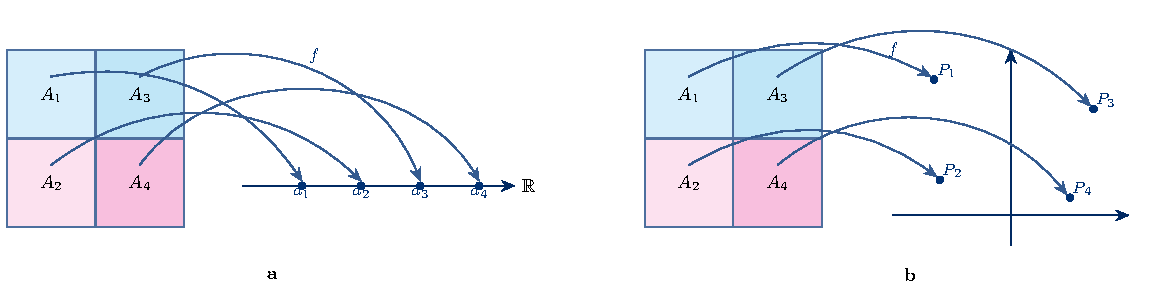
\includegraphics[max width=\linewidth]{Fig36.pdf} 
\caption{Mapa de decisión asociado a una partición: {\bf a}. El espacio de etiquetas es $\R$. {\bf b}. El espacio de etiquetas es $\R^2$.}
\label{fig36}
\end{figure}

En ocasiones, en vez de considerar $N$ vectores linealmente independientes en $\R^N$ se consideran $N$ puntos en $\R^N$ notados por $\pp_1,\dots,\pp_N$. Al usar puntos como etiquetas necesitamos que los mismos sean {\em afínmente independientes}, es decir, linealmente independientes pero no necesariamente vistos como vectores con origen en el origen de coordenadas. Para entender este concepto damos una definición y un resultado asociado. (Notemos que $N$ puntos afínmente independientes generan un espacio afín de dimensión $N-1$, de modo que $N-1$ coordenadas bastan para describir las etiquetas.)

\begin{defi}
Decimos que $E\subset \R^N$ es un {\em espacio afín}, si existe $\pp_0\in \R^N$ y $\Sb\subset \R^N$ subespacio, tal que $E=\Sb + \pp_0$. 
\end{defi}

\begin{prop}
Sea $E$ un espacio afín. Asumamos que $E =\Sb + \pp = \Tb + \qq$ donde $\Sb$ y $\Tb$ son dos subespacios de $\R^N$ y $\pp$, $\qq$ son puntos de $\R^N$. Entonces $\Sb = \Tb$ y $\pp, \qq\in E$.
\end{prop}

Es decir, el subespacio que caracteriza al espacio afín es único.

\begin{proof}
Si $E = \Sb + \pp$ con $\Sb\subset \R^N$ un subespacio, entonces $\pp = 0+\pp\in E$ dado que $0\in\Sb$.

Ahora, si tenemos que $\Sb + \pp = \Tb + \qq$, se tiene que $0+\pp = t + \qq$ para algún $t\in\Tb$. De donde sigue que $\pp-\qq = t\in \Tb$. Análogamente, $\pp-\qq\in \Sb$. 

Finalmente, si $s\in \Sb$, entonces existe $t \in \Tb$ tal que $s+\pp = t+\qq$, de donde $s = t + (\pp-\qq)\in \Tb$. Es decir $\Sb\subset \Tb$. Por simetría, $\Tb\subset \Sb$ lo que finaliza la demostración.
\end{proof}

\begin{defi}
Sea $E$ un espacio afín, $E=\Sb + \pp$ con $\Sb\subset \R^N$ un subespacio. Se define la dimensión del espacio afín $E$ como la dimensión del subespacio $\Sb$. Es decir
$$
\dim E = \dim \Sb.
$$
\end{defi}

\begin{obs}\label{obs.unico}
Observemos que dados $\{\pp_1,\dots,\pp_N\}\subset \R^N$ si definimos el subespacio $\Sb$ como
$$
\Sb = \text{gen}\{\pp_2-\pp_1,\dots,\pp_N-\pp_1\},
$$
entonces $\{\pp_1,\dots,\pp_N\}\subset E = \Sb + \pp_1$, y tenemos que
$$
\dim E = \dim \Sb\le N-1.
$$
\end{obs}

\begin{defi}
Sean $\pp_1,\dots,\pp_N\in \R^N$. Decimos que $\{\pp_1,\dots,\pp_N\}$ es {\em afínmente independiente} si no existe un subespacio afín de dimensión menor que $N-1$ que los contenga.
\end{defi}

Es fácil ver que si $\{\pp_1,\dots,\pp_N\}$ es afínmente independiente, el subespacio afín que los contiene (que tiene dimensión $N-1$) es único (ver el Ejercicio \ref{18.11.3}).

La siguiente proposición caracteriza a los puntos afínmente independientes.
\begin{prop}\label{equiv.afin}
Sean $\pp_1,\dots,\pp_N\in \R^N$. Entonces $\{\pp_1,\dots,\pp_N\}$ es afínmente independiente si y sólo si existe $\pp_0\in\R^N$ tal que el conjunto $\{\pp_1-\pp_0,\dots,\pp_N-\pp_0\}$ es linealmente independiente.
\end{prop}
 
 \begin{proof}
 Asumamos que $\{\pp_1,\dots,\pp_N\}$ es afínmente independiente y sea $E$ el subespacio afín de dimensión $N-1$ que los contiene, $E=\Sb + \qq$ para algún $\qq\in\R^N$ y $\Sb$ un hiperplano. Sea $\pp_0\in \R^N\setminus E$. Veamos entonces que el conjunto $\{\pp_1-\pp_0,\dots,\pp_N-\pp_0\}$ es linealmente independiente. 

Sean $c_1,\dots, c_N\in \R$ tales que
$$
\sum_{j=1}^N c_j (\pp_j-\pp_0) = 0.
$$
Debemos ver que $c_1=\cdots=c_N=0$.

Ahora,
$$
0 = \sum_{j=1}^N c_j (\pp_j-\pp_0) = \left(\sum_{j=1}^N c_j\right) (\pp_1-\pp_0) + \sum_{j=2}^N c_j (\pp_j - \pp_1).
$$ 
 
Por la Observación \ref{obs.unico} sabemos que el conjunto $\{\pp_2-\pp_1,\dots,\pp_N-\pp_1\}$ es linealmente independiente y es un sistema de generadores de $\Sb$. 

Como $\pp_0\not\in E$, sigue que $\pp_1 -\pp_0\not\in \Sb$. Luego $\pp_1-\pp_0$ es linealmente independiente del conjunto $\{\pp_2-\pp_1,\dots,\pp_N-\pp_1\}$ de donde obtenemos que 
$$
\left(\sum_{j=1}^N c_j\right) = c_2 = \cdots = c_N = 0
$$
y por lo tanto también $c_1=0$, que es lo deseado.

Supongamos ahora que existe $\pp_0\in\R^N$ tal que $\{\pp_1-\pp_0,\dots,\pp_N-\pp_0\}$ es linealmente independiente. Debemos ver que el conjunto $\{\pp_1,\dots,\pp_N\}$ es afínmente independiente. Sea $\Sb$ el subespacio generado por $\{\pp_2-\pp_1,\dots,\pp_N-\pp_1\}$, entonces $\{\pp_1,\dots,\pp_N\}\subset E = \Sb + \pp_1$. Veamos que $\dim\Sb=N-1$ o, equivalentemente, que $\{\pp_2-\pp_1,\dots,\pp_N-\pp_1\}$ es linealmente independiente. Sean $c_2,\dots,c_N\in\R$ tales que
$$
\sum_{j=2}^N c_j (\pp_j-\pp_1) = 0.
$$
Pero de acá obtenemos que
$$
0 = \sum_{j=2}^N c_j (\pp_j-\pp_1) = \sum_{j=2}^N c_j (\pp_j-\pp_0) -  \left(\sum_{j=2}^N c_j\right) (\pp_1-\pp_0).
$$
Como el conjunto $\{\pp_1-\pp_0,\dots,\pp_N-\pp_0\}$ es linealmente independiente, deducimos que
$$
c_2 = \cdots = c_N = \left(\sum_{j=2}^N c_j\right) = 0,
$$
de donde $c_2 = \cdots = c_N = 0$ como queríamos demostrar.
\end{proof}

Así como los espacios afines definen traslaciones de subespacios, las transformaciones afines son traslaciones de transformaciones lineales.
\begin{defi}
Decimos que $f\colon \R^N\to\R^N$ es una transformación afín si existe $g\colon \R^N\to\R^N$ transformación lineal y $\pp\in\R^N$ tal que
$$
f(\xx) = g(\xx) + \pp,\qquad \forall \xx\in\R^N.
$$
\end{defi}

Con la ayuda de la Proposición \ref{equiv.afin} podemos definir una transformación afín biyectiva entre vectores one-hot y puntos afínmente independientes.
\begin{prop}
Sea $\{\pp_1,\dots,\pp_N\}\subset \R^N$ afínmente independiente. Entonces existe una transformación afín $f\colon \R^N\to\R^N$ biyectiva tal que $f(\pp_j)=\ee_j$ para $j=1,\dots,N$.
\end{prop}

\begin{proof}
Sea $\pp_0\in\R^N$ tal que el conjunto $\{\pp_1-\pp_0,\dots,\pp_N-\pp_0\}$ es linealmente independiente. Luego, existe una única transformación lineal $g\colon \R^N\to\R^N$ tal que $g(\pp_j-\pp_0)=\ee_j$. Esta transformación lineal resulta inversible y la inversa viene dada por la única transformación lineal que verifica $g^{-1}(\ee_j) = \pp_j-\pp_0$ para $j=1,\dots,N$.

Ahora, definimos $f(\xx) = g(\xx-\pp_0) = g(\xx) - g(\pp_0) = g(\xx) + \pp$ (donde $\pp=-g(\pp_0))$. Luego $f$ es una transformación afín, $f(\pp_j) = g(\pp_j-\pp_0)=\ee_j$ y $f$ es inversible con
$$
f^{-1}(\xx) = g^{-1}(\xx) + \pp_0,
$$
lo que finaliza la demostración.
\end{proof}

\section{Separabilidad lineal}\label{sec.c10.5}

Un cluster de puntos en $\R^n$ es un conjunto $\G = \{\xx_1,\dots,\xx_k\}$ que suponemos posee cierta característica que lo distingue. Dos clusters en $\R^n$, $\G_1$ y $\G_2$, se dicen {\em linealmente separables} si existe un hiperplano $\Hc$ que los separa. Esto significa
\begin{itemize}
\item[(i)] El hiperplano $\Hc$ (espacio afín de dimensión $n-1$) determina dos semi-espacios abiertos disjuntos $S_1$ y $S_2$ (los dos lados de $\Hc$).
\item[(ii)] Cada cluster está contenido en uno de estos semi-espacios: $\G_1\subset S_1$ y $\G_2\subset S_2$.
\end{itemize}
Asumamos que el hiperplano está definido implícitamente por la ecuación
$$
h(\xx) = a_1 x_1 + \cdots + a_n x_n + d = 0,
$$
entonces la separabilidad de $\G_1$ y $\G_2$ se puede escribir como $h(g_1)h(g_2)<0$ para todo par de puntos $g_i\in \G_i$, $i=1, 2$.

Al estudiar el problema de la separación lineal de clusters es conveniente entender el conjunto que encierra un cluster dado. Para eso necesitaremos algunas definiciones.
\begin{defi}
Un conjunto $K\subset \R^n$ se dice convexo si para todo par de puntos $\xx, \yy\in K$, el segmento de puntos que une $\xx$ con $\yy$ y que denotamos por
$$
[\xx, \yy] = \{ t\xx + (1-t)\yy\colon t\in [0,1]\},
$$
está contenido en $K$.
\end{defi}

En general un cluster no es un conjunto convexo. Entonces necesitamos considerar al menor conjunto convexo que lo contiene.
\begin{defi}
Sea $A\subset\R^n$ un conjunto no vacío. Definimos la cápsula convexa de $A$, y la notamos como $\hull(A)$ al menor conjunto convexo que contiene a $A$, es decir
$$
\hull(A) = \bigcap_{{A\subset K}\atop{K \text{ convexo}}} K
$$
\end{defi}

Observamos que, como $\R^n$ es convexo, siempre existe un convexo conteniendo a cualquier conjunto y que la intersección de un número arbitrario de convexos es convexo (verificar esto). Luego $\hull(A)$ está efectivamente bien definido, es convexo y es el convexo más chico (en el sentido de la inclusión) que contiene a $A$.

Cuando el conjunto $A$ es un cluster formado por finitos elementos, $A=\G=\{\xx_1,\dots,\xx_k\}$, se tiene una caracterización de su cápsula convexa $\hull(\G)$.
\begin{prop}\label{prop1053}
Sea $\G=\{\xx_1,\dots,\xx_k\}\subset \R^n$. Entonces
$$
\hull(\G) = \left\{\sum_{i=1}^k \lambda_i \xx_i\colon \sum_{i=1}^k \lambda_i = 1,\ \lambda_i\ge 0\right\}.
$$
\end{prop}

Es decir, la cápsula convexa de $\G$ es el conjunto de todas las {\em combinaciones convexas} de elementos del $\G$. La demostración de esta proposición está contenida en el Ejercicio \ref{18.11.5}.

Tenemos el siguiente resultado.
\begin{prop}
Sean $\G_1, \G_2\subset \R^n$ dos clusters. Entonces $\G_1$ y $\G_2$ son linealmente separables si y sólo si sus cápsulas convexas $\hull(\G_1)$ y $\hull(\G_2)$ lo son.
\end{prop}

\begin{proof}
Es claro que si $\hull(\G_1)$ y $\hull(\G_2)$ son linealmente separables, entonces $\G_1$ y $\G_2$ también lo son, dado que $\G_i\subset \hull(\G_i)$, $i=1, 2$. Ver la Figura \ref{fig37}

\begin{figure}[htbp]
\centering
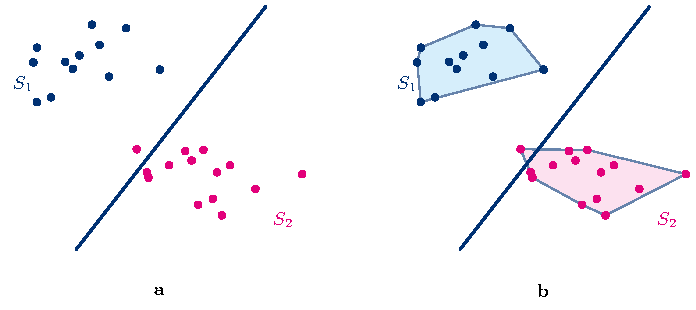
\includegraphics[max width=\linewidth]{Fig37.pdf} 
\caption{{\bf a}. Separación lineal de dos clusters. {\bf b}. Separación lineal de las cápsulas convexas de dos clusters.}
\label{fig37}
\end{figure}

Supongamos ahora que $\G_1$ y $\G_2$ son linealmente separables. Entonces tenemos dos semi-espacios abiertos disjuntos $S_1$ y $S_2$ tales que $\G_i\subset S_i$, $i=1, 2$. Pero cada semi-espacio es un conjunto convexo que contiene al cluster, y como la cápsula convexa es el menor conjunto convexo que contiene al cluster deducimos que $\hull(\G_i)\subset S_i$, $i=1, 2$.
\end{proof}

En el Ejercicio \ref{18.11.9} se ve que $\G_1$ y $\G_2$ son linealmente separables si y sólo si $\hull(\G_1)\cap \hull(\G_2)=\emptyset$.


Si dos clusters no son linealmente separables, entonces no es posible {\em separarlos} usando transformaciones lineales.
\begin{prop}
Sean $\G_1, \G_2\subset \R^n$ dos clusters tales que $\hull(\G_1)\cap \hull(\G_2)\neq\emptyset$. Entonces si $F\colon \R^n\to\R^p$ es una transformación lineal, tenemos que $F(\G_1)$ y $F(\G_2)$ no son linealmente separables.
\end{prop} 

\begin{proof}
Asumamos, por el absurdo, que existe $F\colon \R^n\to\R^p$ transformación lineal tal que $F(\G_1)$ y $F(\G_2)$ son linealmente separables. 

Sea $h(\xx) = \sum_{i=1}^p a_i x_i + d=0$ la ecuación implícita del hiperplano $\Hc$ que separa $F(\G_1)$ y $F(\G_2)$. Luego, si $g_i\in \G_i$, $i=1, 2$, tenemos que
$$
h(F(g_1))h(F(g_2)) < 0.
$$

Sea ahora $g\in \hull(\G_1)\cap\hull(\G_2)$, luego, $g$ admite las representaciones
$$
g=\sum_{i=1}^{k_1} \lambda_i^1 g_i^1 = \sum_{j=1}^{k_2}\lambda_j^2 g_j^2,
$$
donde $g_i^1\in \G_1$, $g_j^2\in \G_2$, $\lambda_i^1, \lambda_j^2\ge 0$ y $\sum_{i=1}^{k_1}\lambda_i^1 = \sum_{j=1}^{k_2}\lambda_j^2 = 1$.

Si usamos ahora la linealidad de $F$ y observando que $h$ distribuye las combinaciones convexas, obtenemos
\begin{align*}
0\le \left[h(F(g))\right]^2 & = h(F(g)) h(F(g))\\
&= h\left(F\left(\sum_{i=1}^{k_1} \lambda_i^1 g_i^1\right)\right) h\left(F\left(\sum_{j=1}^{k_2} \lambda_j^2 g_j^2\right)\right)\\
&= \left(\sum_{i=1}^{k_1} \lambda_i^1 h(F(g_i^1))\right) \left(\sum_{j=1}^{k_2} \lambda_j^2 h(F(g_j^2))\right)\\
&= \sum_{i=1}^{k_1}\sum_{j=1}^{k_2} \lambda_i^1\lambda_j^2 h(F(g_i^1)) h(F(g_j^2)) < 0.
\end{align*}
Esto es una contradicción y la demostración está completa.
\end{proof}


\begin{obs}
\begin{enumerate}
\item[(i)] Vale la pena notar que tampoco existe una función de separación que sea afín, es decir, de la forma $F(x) = Wx + b$, donde $W$ es una matriz $p \times n$ y $b \in \R^p$. En efecto, la demostración anterior vale también para aplicaciones afines $F$, porque $h\circ F$ es una función afín y por lo tanto también ``distribuye'' las combinaciones convexas. En consecuencia, una neurona lineal no puede separar dos clusters cuyas cápsulas convexas se intersecan. Para esta tarea, debemos emplear redes neuronales con funciones de activación no lineales.

\item[(ii)] Dos clusters en $\R^n$, $\G_1$ y $\G_2$, se llaman {\em $F-$separables} si existe una aplicación bi-continua e invertible $F\colon \R^n \to \R^n$ tal que las imágenes de los clusters, $F(\G_1)$ y $F(\G_2)$, son separables linealmente en $\R^n$. Dicha función $F$ se llama un {\em homeomorfismo de} $\R^n$.

Por el teorema de Cybenko (Capítulo~\ref{cap9}), una {\em red neuronal feedforward} con una capa oculta puede aproximar uniformemente en un compacto cualquier función continua $F$. Como la separabilidad lineal estricta de clusters finitos es una condición abierta (se preserva si se perturba $F$ poco), basta aproximar $F$ y no hace falta reproducirla exactamente, ni que sea un homeomorfismo. Si además agregamos un perceptrón, podemos realizar la clasificación lineal final. De esta manera, un problema de clasificación se reduce al aprendizaje de la función continua no lineal $F$. (Para $n\ge2$ y clusters finitos disjuntos siempre existe un homeomorfismo de $\R^n$ que los vuelve linealmente separables, pues los homeomorfismos de $\R^n$, $n\ge2$, pueden llevar cualquier colección finita de puntos distintos en cualquier otra; para $n=1$ no, porque los homeomorfismos de $\R$ son monótonos y preservan el orden.)

\item[(iii)] El papel de la función $F$ es {\em separar los clusters}, de modo que puedan clasificarse linealmente. Sin embargo, hay casos (con conjuntos infinitos) en los que los clusters no pueden separarse mediante un homeomorfismo de $\R^n$. En este caso, necesitamos una dimensión extra para separar los clusters, y la función continua debe ser $F\colon \R^n \to \R^p$, con $p > n$. 

Por ejemplo, los conjuntos
$$
\G_1 = \{ x \in \R^2\colon  \|x\| < 1 \}, \quad \G_2 = \{ x \in \R^2\colon \|x\| > 2 \}
$$
no pueden separarse linealmente mediante un homeomorfismo $F$ de $\R^2$: $F(\G_2)=\R^2\setminus F(\{\|x\|\le2\})$ es el complemento de un compacto y no puede estar contenido en un semiplano. En cambio, sí pueden separarse en $\R^3$ con la función continua (no homeomorfismo) $F(x)=(x,\|x\|^2)$: $F(\G_1)$ queda en $\{z<1\}$ y $F(\G_2)$ en $\{z>4\}$, separados por el plano $z=\frac52$.
\end{enumerate}
\end{obs}

\begin{obs}
Cuando se tienen $k$ clusters, $\G_1,\dots,\G_k$, decimos que son separables linealmente {\em dos a dos} si $\G_i$ y $\G_j$ son linealmente separables para todo $i\neq j$, $i, j=1,\dots, k$. Esto es más débil que pedir que cada $\G_i$ sea separable de la unión de todos los demás (``uno contra todos''). Por ejemplo, los tres clusters $\G_y=\{(-10,y),(0,y),(10,y)\}$, $y=-1,0,1$, son separables dos a dos (sus cápsulas convexas son tres segmentos horizontales paralelos), pero $\G_0$ no es separable linealmente de $\G_1\cup\G_{-1}$, pues $(0,0)$ es el punto medio de $(0,1)$ y $(0,-1)$.
\end{obs}

\section{Separabilidad convexa}\label{sec.c10.6}

La separabilidad puede ser considerada en una manera levemente diferente, pero equivalente. Una familia de clusters $\Gk = \{\G_1,\dots,\G_k\}$ en $\R^n$ se dice {\em separable convexamente} si existen $k$ bolas cerradas $B_1,\dots, B_k$ en $\R^n$ tales que
\begin{itemize}
\item[(i)] $B_i\cap B_j=\emptyset$ para todo $i\neq j$;
\item[(ii)] $\G_j\subset B_j$, $j=1,\dots,k$.
\end{itemize}

Veamos que los conceptos de separabilidad convexa y lineal son equivalentes. Para eso necesitamos un lema.
\begin{lema}\label{Bola.semiespacio}
Sea $S\subset \R^n$ el semiespacio definido como $S=\{\xx\in \R^n\colon x_1>0\}$. Entonces
$$
S = \bigcup_{m=1}^\infty B_m(m\ee_1),
$$
donde $B_r(\xx_0)$ denota la bola abierta de radio $r>0$ centrada en $\xx_0\in\R^n$.
\end{lema}

\begin{proof}
Observemos primero que $B_m(m\ee_1)\subset S$ para todo $m\in\N$. Ver Figura \ref{fig38}.

Sea ahora $\xx\in S$. Escribimos $\xx=(x_1, \xx')$ con $x_1>0$ y $\xx'\in\R^{n-1}$.
Veamos que $\xx\in B_m(m\ee_1)$ si $m$ es suficientemente grande. Pero
\begin{align*}
\|\xx-m\ee_1\|^2 &= (x_1-m)^2 + |\xx'|^2 = m^2 - 2m x_1 + x_1^2+|\xx'|^2\\
&= m^2-m\left(2x_1 - \frac{x_1^2 + |\xx'|^2}{m}\right)<m^2,
\end{align*}
si 
$$
2x_1 - \frac{x_1^2 + |\xx'|^2}{m} >0 \quad \text{o, equivalentemente, si }\quad m>\frac{x_1^2 + |\xx'|^2}{2x_1}.
$$
Esto termina la demostración.
\end{proof}

\begin{figure}[htbp]
\centering
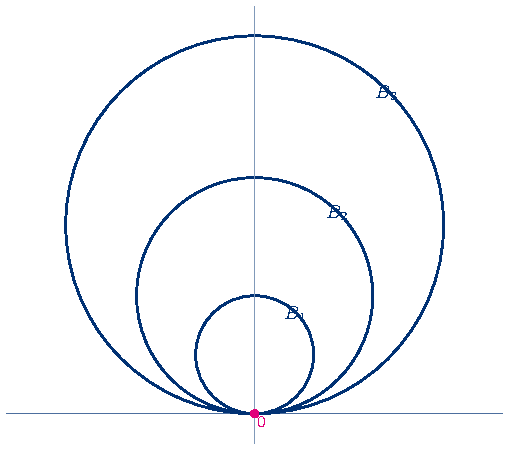
\includegraphics[max width=\linewidth]{Fig38.pdf} 
\caption{Las bolas de la sucesión en la demostración del Lema \ref{Bola.semiespacio}}
\label{fig38}
\end{figure}

\begin{cor}\label{K.en.bola}
Sea $K\subset \R^n$ un conjunto compacto y sea $S\subset \R^n$ un semi-espacio tal que $K\subset S$. Entonces, existe una bola $B\subset S$ tal que $K\subset B$.
\end{cor}

\begin{proof}
Aplicando una rotación y una traslación, podemos suponer sin pérdida de generalidad que $S=\{\xx\in\R^n\colon x_1>0\}$.

Luego, por el Lema \ref{Bola.semiespacio}, tenemos que
$$
K\subset S = \bigcup_{m=1}^\infty B_m(m\ee_1).
$$
La sucesión de bolas es creciente (ver Figura \ref{fig38}), es decir, $B_m(m\ee_1)\subset B_{m+1}((m+1)\ee_1)$. En efecto, si $\|\xx-m\ee_1\|<m$, entonces $x_1>0$ y
$$
\|\xx-(m+1)\ee_1\|^2=\|\xx-m\ee_1\|^2-2x_1+2m+1<(m+1)^2-2x_1<(m+1)^2.
$$
Ahora bien, como $\{B_m(m\ee_1)\}_{m\in\N}$ es un cubrimiento por abiertos de $K$ que es compacto, existen $m_1<\cdots< m_k$ finitos, tales que
$$
K\subset \bigcup_{j=1}^k B_{m_j}(m_j\ee_1).
$$
Pero como la sucesión de bolas es creciente, $K\subset B_{m_k}(m_k \ee_1)\subset S$.
\end{proof}

Estamos ahora en condiciones de demostrar la equivalencia entre las nociones de separabilidad.
\begin{prop}\label{sep.equiv}
Dos clusters $\G_1$ y $\G_2$ en $\R^n$ son convexamente separables si y sólo si son linealmente separables.
\end{prop}

\begin{proof}
Supongamos que $\G_1$ y $\G_2$ son separados convexamente. Entonces tenemos $B_1$ y $B_2$ dos bolas tales que $\G_i\subset B_i$, $i=1, 2$, con $B_1\cap B_2=\emptyset$. Luego, consideramos el hiperplano $\Hc$ que tiene como normal al vector que une los centros de esas bolas y que pasa por un punto del segmento que une esos centros que esté fuera de ambas bolas. Claramente $\Hc$ separa $\G_1$ y $\G_2$.

El recíproco es una consecuencia inmediata del Corolario \ref{K.en.bola}. En efecto, si $\G_1$ y $\G_2$ son linealmente separables, entonces tenemos un hiperplano $\Hc$ que separa $\hull(\G_1)$ y $\hull(\G_2)$. Como las cápsulas convexas son compactas, por el Corolario \ref{K.en.bola} existen bolas $\tilde B_i$, $i=1, 2$, contenidas en cada semi-espacio determinado por $\Hc$ tales que $\hull(\G_i)\subset \tilde B_i$, $i=1,2$. Ahora, tomando una bola cerrada de mismo centro y radio levemente inferior, $B_i\subset \tilde B_i$, $i=1,2$ se obtiene lo pedido.
\end{proof}

\begin{obs}
El concepto de separabilidad convexa es en apariencia más robusto y fácil de interpretar geométricamente, pero el de separabilidad lineal es el más sencillo de atacar usando redes neuronales. La Proposición \ref{sep.equiv} nos garantiza la equivalencia.
\end{obs}

La equivalencia de la Proposición \ref{sep.equiv} es para {\em dos} clusters. Si $k\ge3$, la separabilidad lineal dos a dos {\em no} implica que existan $k$ bolas cerradas disjuntas $B_j\supset\G_j$. En el ejemplo de la observación anterior, $\G_y=\{(-10,y),(0,y),(10,y)\}$, $y=-1,0,1$: un disco $B_0\supset\G_0$ contiene a $(\pm10,0)$, y por la potencia del punto $(0,0)$ respecto de su circunferencia la cuerda de $B_0$ sobre la recta $x=0$ tiene segmentos $|MU|,|MV|$ a cada lado de $(0,0)$ con $|MU|\,|MV|\ge10\cdot10=100$; luego uno de ellos es mayor que $1$ y $B_0$ contiene a $(0,1)\in\G_1$ o a $(0,-1)\in\G_{-1}$. Entonces $B_0$ interseca a $B_1$ o a $B_{-1}$.

Sin embargo, la existencia de un mapa de decisión continuo es automática para clusters finitos disjuntos, sin ninguna hipótesis de separabilidad:
\begin{prop}
Sea $\Gk = \{\G_1,\dots,\G_k\}$ una familia de $k$ clusters finitos de $\R^n$, disjuntos dos a dos. Entonces existe una función continua $F\colon \R^n\to \R^k$ tal que $F(\G_j)= \ee_j$, $j=1,\dots,k$.
\end{prop}

\begin{proof}
Sea $\G=\bigcup_j\G_j$ (un conjunto finito) y sea $\delta>0$ la menor distancia entre dos puntos distintos de $\G$. Para $\yy\in\G_j$ sea $\varphi_{\yy}(\xx)=\max\{0,1-2\|\xx-\yy\|/\delta\}$, que es continua, vale $1$ en $\yy$ y se anula en $\G\setminus\{\yy\}$. Definimos $F(\xx)=\sum_{j=1}^k\sum_{\yy\in\G_j}\varphi_{\yy}(\xx)\,\ee_j$.
\end{proof}

La separabilidad es importante, en cambio, cuando se exige que la clasificación se haga con aplicaciones simples (lineales, o con pocas neuronas) y no sólo por memorización de los puntos.

\section{Contracción al centro}\label{sec.c10.7}

Para poder separar clusters es usual tener que aplicar transformaciones que los contraiga hacia ciertos puntos que será luego utilizados como etiquetas.

Empecemos con el caso simple de un único cluster que es llevado hacia un punto llamado {\em centro}. Consideremos $\G = \{\xx_1,\dots,\xx_k\}\subset \R^n$ un cluster y $\cc\in\R^n$ otro punto que llamaremos el centro.

Definimos entonces la transformación dada por
$$
\yy_j = \lambda\xx_j + (1-\lambda)\cc, \quad \lambda\in (0,1).
$$
Para cada valor de $\lambda$ fijo, esta transformación contrae el cluster $\G$ hacia otro cluster $\G^\lambda$ situado en una proximidad del centro $\cc$. Ver Figura \ref{fig39} {\bf a}. A valores más pequeños de $\lambda$, más cerca del centro $\cc$ estará el cluster $\G^\lambda$.

\begin{figure}[htbp]
\centering
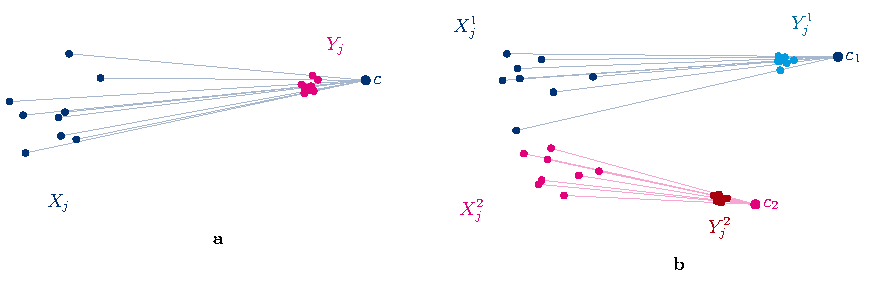
\includegraphics[max width=\linewidth]{Fig39.pdf} 
\caption{{\bf a}. Contracción de un cluster hacia un punto. {\bf b}. Contracción de dos clusters hacia dos puntos distintos.}
\label{fig39}
\end{figure}

Consideremos ahora dos clusters $\G_1$ y $\G_2$ y dos centros distintos $\cc_1$ y $\cc_2$. Notemos $\G_1 = \{\xx_1^1,\dots,\xx_{k_1}^1\}$ y $\G_2= \{\xx_1^2,\dots,\xx_{k_2}^2\}$ y definimos las transformaciones
\begin{align*}
\yy_i^1 &= \lambda_1 \xx_i^1 + (1-\lambda_1) \cc_1,\quad i=1,\dots,k_1\\
\yy_j^2 &= \lambda_2 \xx_j^2 + (1-\lambda_2) \cc_2,\quad j=1,\dots,k_2.
\end{align*}
Estas transformaciones empujan cada cluster hacia su respectivo centro. Ver Figura \ref{fig39} {\bf b}. Si $\|\xx-\cc_i\|\le\rho_i$ para todo $\xx\in\G_i$, entonces $\G_i^{\lambda_i}$ está contenido en la bola cerrada de centro $\cc_i$ y radio $\lambda_i\rho_i$. Por lo tanto, si $\lambda_1\rho_1+\lambda_2\rho_2<\|\cc_1-\cc_2\|$, los nuevos clusters $\G_1^{\lambda_1}$ y $\G_2^{\lambda_2}$ quedan en bolas disjuntas y, en particular, son linealmente separables (aunque los originales no lo fueran). Para valores de $\lambda_i$ cercanos a $1$ no hay en general ninguna mejora.

Estas transformaciones están en principio sólo definidas sobre los puntos de los clusters. La dificultad radica en si es posible extender estas transformaciones a funciones definidas globalmente. Para clusters finitos disjuntos siempre es posible, por ejemplo mediante una función continua como la de la proposición anterior (o por el teorema de extensión de Tietze), y por el teorema de Cybenko una red con una capa oculta puede aproximarla uniformemente en un compacto. En la sección siguiente consideramos los casos más sencillos, en que el mapa de decisión se busca lineal (sin capas ocultas) o dado por una red pequeña.


\section{Aprendiendo mapas de decisión}\label{sec.c10.8}

La clasificación de clusters se alcanza aprendiendo mapas de decisión. En esta sección estudiaremos este tema.

\subsection{Mapas de decisión lineales}

Consideremos dos clusters en $\R^2$,
$$
\G = \{(x_1,y_1),\dots,(x_N, y_N)\} \quad \text{y}\quad \bar\G = \{(\bar x_1,\bar y_1),\dots,(\bar x_M, \bar y_M)\},
$$
y asumamos que los clusters son linealmente separables, equivalentemente (ver el Ejercicio \ref{18.11.9}), que $\hull(\G)\cap\hull(\bar\G)=\emptyset$. Estudiemos los casos de espacios de etiquetas de dimensión uno y dos.

\subsubsection*{Etiquetas unidimensionales} Asociamos dos etiquetas, $\alpha$ y $\bar\alpha$ a cada uno de los clusters $\G$ y $\bar\G$ respectivamente. Como los clusters son linealmente separables resulta razonable buscar una función lineal $f\colon\R^2\to\R$ que lleve el cluster $\G$ a un entorno de $\alpha$ y el cluster $\bar\G$ a un entorno de $\bar\alpha$. Esperamos también que el punto medio, $\frac{\alpha+\bar\alpha}{2}$, separe los conjuntos $f(\G)$ y $f(\bar\G)$.

Luego, buscamos $f$ de la forma
$$
f(x,y)=f_{\ww, b}(x, y) = w_1 x + w_2 y + b.
$$
Es decir, $f$ es la función de entrada-salida de una red neuronal feedforward con salida unidimensional sin capas ocultas. Los parámetros $\ww=(w_1, w_2)$ y $b$ tienen que ser elegidos de forma tal que las imágenes de los clusters $f(\G)$ y $f(\bar\G)$ estén localizados en un entorno de $\alpha$ y $\bar\alpha$ respectivamente. Para lograr eso, se toma
$$
(\ww, b) = \argmin F(\ww, b),
$$
donde $F$ es la función de costo cuadrático dada por
\begin{align*}
F(\ww, b) &= \frac12 \sum_{i=1}^N (f_{\ww, b}(x_i, y_i)-\alpha)^2 + \frac12 \sum_{j=1}^M (f_{\ww, b}(\bar x_j, \bar y_j)-\bar\alpha)^2\\
&= \frac12 \sum_{i=1}^N (w_1 x_i + w_2 y_i + b - \alpha)^2 + \frac12 \sum_{j=1}^M (w_1 \bar x_j + w_2 \bar y_j + b-\bar\alpha)^2.
\end{align*}

El mínimo del costo $F$, se alcanza cuando $\nabla F=0$. Calculemos entonces el gradiente $\nabla F=(\partial_{w_1} F, \partial_{w_2}F, \partial_b F)$. Este cálculo se realiza con una aplicación inmediata de la regla de la cadena:
\begin{align*}
\partial_{w_1} F =&\ w_1\left(\sum_{i=1}^N x_i^2 + \sum_{j=1}^M \bar x_j^2\right) + w_2\left(\sum_{i=1}^N x_i y_i + \sum_{j=1}^M \bar x_j \bar y_j\right)\\
& + b\left(\sum_{i=1}^N x_i + \sum_{j=1}^M \bar x_j\right) - \alpha\sum_{i=1}^N x_i - \bar\alpha \sum_{j=1}^M \bar x_j
\end{align*}
\begin{align*}
\partial_{w_2} F =&\ w_1 \left(\sum_{i=1}^N x_i y_i + \sum_{j=1}^M \bar x_j \bar y_j\right)+ w_2\left(\sum_{i=1}^N y_i^2 + \sum_{j=1}^M \bar y_j^2\right)\\
& + b\left(\sum_{i=1}^N y_i + \sum_{j=1}^M \bar y_j\right) - \alpha\sum_{i=1}^N y_i - \bar\alpha \sum_{j=1}^M \bar y_j\\
\partial_b F =&\ w_1\left(\sum_{i=1}^N x_i + \sum_{j=1}^M \bar x_j\right) + w_2\left(\sum_{i=1}^N y_i + \sum_{j=1}^M \bar y_j\right)\\
&+ (N+M) b - N\alpha - M\bar\alpha.
\end{align*}
En base a estos cálculos, obtener $\nabla F=0$ es un problema de álgebra lineal. Escribamos las matrices involucradas. 
\begin{equation}\label{A.barA}
A = \begin{pmatrix}
\sum x_i^2 & \sum x_i y_i & \sum x_i\\
\sum x_i y_i  & \sum y_i^2 & \sum y_i\\
\sum x_i & \sum y_i & N
\end{pmatrix},\qquad 
\bar A = \begin{pmatrix}
\sum \bar x_j^2 & \sum \bar x_j \bar y_j & \sum \bar x_j\\
\sum \bar x_j \bar y_j  & \sum \bar y_j^2 & \sum \bar y_j\\
\sum \bar x_j & \sum \bar y_j & M
\end{pmatrix}.
\end{equation}
Estas matrices $A$ y $\bar A$ contienen la información de los clusters $\G$ y $\bar\G$ respectivamente. Sus entradas son los primeros y segundos momentos de las variables $x$ e $y$ de los datos y su correlación. Consideremos ahora los vectores
$$
\beta = \alpha\begin{pmatrix}
\sum x_i\\ 
\sum y_i\\
N
\end{pmatrix},\qquad
\bar\beta = \bar\alpha\begin{pmatrix}
\sum \bar x_j\\ 
\sum \bar y_j\\
M
\end{pmatrix},
$$
que dependen de las etiquetas y de los primeros momentos de los datos. Luego, la ecuación $\nabla F=0$ se escribe como
$$
(A+\bar A) X = \beta + \bar\beta,
$$
donde $X=(w_1, w_2, b)^T$. La matriz $A+\bar A$ es la matriz de Gram de los puntos extendidos $(x,y,1)$ (es decir, $A+\bar A=\Phi^T\Phi$, donde las filas de $\Phi$ son los $(x_i,y_i,1)$ y los $(\bar x_j,\bar y_j,1)$) y es inversible si y sólo si los $N+M$ puntos no son colineales; en ese caso la solución es única.

La resolución de esta ecuación se puede realizar por varios métodos como los que estudiaron en Álgebra Lineal Computacional o en Elementos de Cálculo Numérico (ver también el Apéndice G de \cite{Calin}).

Las etiquetas $\alpha$ y $\bar\alpha$ consideradas pueden tomarse, por simplicidad, como $\alpha=1$ y $\bar\alpha = 0$.

\begin{obs}
El ajuste por mínimos cuadrados a las etiquetas {\em no} garantiza clasificar bien, aun cuando los clusters sean linealmente separables. Por ejemplo, en $\R$ tomemos $\G=\{-1,-0.9\}$ con etiqueta $\alpha=1$ y $\bar\G$ formado por el punto $0.1$ y $40$ puntos equiespaciados en $[5,50]$, con etiqueta $\bar\alpha=0$. Los clusters son separables (por $x=-0.4$, por ejemplo), pero el ajuste por mínimos cuadrados da, numéricamente, $f(x)\approx0.192-0.0057\,x$, de modo que $f(\G)\approx0.197<\tfrac12$ y la regla ``$f>\tfrac12\Rightarrow\G$'' clasifica mal los dos puntos de $\G$: los puntos lejanos de $\bar\G$ ``tiran'' de la recta. Con más de dos clusters y etiquetas escalares el problema se agrava, pues las etiquetas imponen un orden entre las clases; por eso se usan etiquetas one-hot y la función softmax. Para datos linealmente separables, el algoritmo del perceptrón encuentra un hiperplano separador en un número finito de pasos (teorema de convergencia de Novikoff, que no demostramos aquí), y la regresión logística con entropía cruzada es la alternativa habitual.
\end{obs}

\subsubsection*{Etiquetas bidimensionales} Vamos a realizar ahora una clasificación de los clusters $\G$ y $\bar\G$ usando etiquetas bidimensionales, tales como vectores o distintos puntos del plano. Asumamos que la etiqueta del cluster $\G$ es el punto $\ab=(a_1, a_2)$ y la etiqueta de $\bar\G$ es el punto $\bar\ab=(\bar a_1, \bar a_2)$.

Como estamos suponiendo que los clusters son linealmente separables, buscamos una función $f\colon \R^2\to\R^2$ lineal que mande $\G$ en un entorno de $\ab$ y $\bar\G$ en un entorno de $\bar\ab$. Esta función lineal $f=(f^1, f^2)$ se construye como la función de entrada-salida de una red neuronal feedforward con una salida de dimensión 2 sin capas ocultas. Esto significa que $f$ es de la forma
\begin{align*}
f^1(x, y) &= f^1_{W, b}(x, y) = w_{11}x + w_{21}y + b_1\\
f^2(x, y) &= f^2_{W, b}(x, y) = w_{12}x + w_{22}y + b_2.
\end{align*}

Los pesos $w_{ij}$ y los sesgos $b_j$ tienen que ser ajustados de manera tal que los conjuntos imagen $f(\G)$ y $f(\bar\G)$ estén lo más próximos posibles a sus etiquetas $\ab$ y $\bar\ab$ respectivamente. Este objetivo se consigue tomando
$$
(W, b) = \argmin G(W, b),
$$
donde $G$ es la suma de los cuadrados de las distancias a las etiquetas, i.e.
\begin{align*}
G(W, b) = &\ \frac12 \sum_{i=1}^N \|f_{W, b}(x_i, y_i) - \ab\|^2 + \frac12 \sum_{j=1}^M \|f_{W, b}(\bar x_j, \bar y_j) - \bar \ab\|^2\\
= &\ \frac12 \sum_{i=1}^N \left[(f^1(x_i, y_i)-a_1)^2 + (f^2(x_i, y_i)-a_2)^2\right]\\
&\ +\frac12 \sum_{j=1}^M \left[(f^1(\bar x_j, \bar y_j)-\bar a_1)^2 + (f^2(\bar x_j, \bar y_j)-\bar a_2)^2\right]\\
= &\ G_1(w_{11}, w_{21}, b_1) + G_2(w_{12}, w_{22}, b_2),
\end{align*}
donde
$$
G_1(w_{11}, w_{21}, b_1) = \frac12 \sum_{i=1}^N (w_{11} x_i+w_{21} y_i + b_1 - a_1)^2 + \frac12\sum_{j=1}^M (w_{11} \bar x_j + w_{21} \bar y_j + b_1 - \bar a_1)^2
$$
$$
G_2(w_{12}, w_{22}, b_2) = \frac12 \sum_{i=1}^N (w_{12} x_i+w_{22} y_i + b_2 - a_2)^2 + \frac12\sum_{j=1}^M (w_{12} \bar x_j + w_{22} \bar y_j + b_2 - \bar a_2)^2
$$
Observemos que ahora tenemos
$$
\nabla G(W, b) = (\nabla G_1(w_{11}, w_{21}, b_1),\nabla G_2(w_{12}, w_{22}, b_2))\in \R^6
$$
y el sistema $\nabla G=0$ se desacopla en $\nabla G_1=0$ y $\nabla G_2=0$ donde cada una de esas ecuaciones está en $\R^3$. Estas ecuaciones en $\R^3$ son las mismas que teníamos en la sección anterior, por lo que las mismas se escriben como
\begin{align*}
(A+\bar A) X_1 &= \beta_1 + \bar\beta_1\\
(A+\bar A) X_2 &= \beta_2 + \bar\beta_2,
\end{align*}
donde $A$ y $\bar A$ vienen dadas por \eqref{A.barA}, $X_k = (w_{1k}, w_{2k}, b_k)^T$, $k=1, 2$ y 
$$
\beta_k = a_k \begin{pmatrix}
\sum x_i\\ 
\sum y_i\\
N
\end{pmatrix},\qquad
\bar\beta_k = \bar a_k\begin{pmatrix}
\sum \bar x_j\\ 
\sum \bar y_j\\
M
\end{pmatrix}, \qquad k=1, 2.
$$
Estas ecuaciones se resuelven de la misma manera que en la sección previa.

\subsubsection*{El uso de la función de activación $\softmax$}
En la mayoría de los problemas de clasificación, se utiliza una capa adicional que implementa la función $\softmax$. Esta función se define como
$$
\softmax\colon \R^m\to\R^m,\quad \softmax(\xx) = \frac{1}{\sum_{i=1}^m e^{x_i}}(e^{x_1},\dots,e^{x_m}).
$$
El objetivo de aplicar esta función es el de normalizar las salidas de la red para entregar un valor en $(0,1)$ para cada coordenada, con suma $1$, de modo que se interprete como una {\em distribución de probabilidad} sobre las clases (la probabilidad de que la entrada pertenezca a la clase $i$, cuyo vector one-hot es $\ee_i$).  Utilicemos esto para el ejemplo de la sección previa tomando como vectores $\ab = \ee_1 = (1, 0)$ y $\bar\ab = \ee_2 = (0,1)$.

La salida de la nueva red será entonces $\zz = (z_1, z_2)$, donde $\zz = \softmax(f)$, es decir
$$
z_i = \frac{e^{f^i}}{e^{f^1} + e^{f^2}},\quad i=1,2.
$$
Como $z_i>0$ y $z_1+z_2=1$ sigue que $\zz$ pertenece al segmento abierto que une los puntos $\ab$ y $\bar\ab$, con la imagen de $\G$ más próxima a $\ab$ y la imagen de $\bar\G$ más próxima a $\bar\ab$. Observemos que las salidas del softmax nunca alcanzan los vértices $\ee_i$ (las coordenadas son siempre estrictamente positivas), por lo que con el costo cuadrático el error nunca se anula; por eso, al usar softmax se entrena con la entropía cruzada $-\sum_i(\ee_{c})_i\ln z_i$, para la cual el gradiente respecto de las señales $\sbf^{(L)}$ de la última capa es $\zz-\ee_c$ (ver el Capítulo~\ref{cap6}).

Asumamos que el punto de separación de los clusters es el punto medio del segmento, $(\tfrac12, \tfrac12)$. Luego, dado un punto $(x, y)\in\R^2$ para decidir a qué cluster pertenece corremos el punto a través de la red neuronal (ver Figura \ref{fig40}) y si la salida pertenece a la parte superior del segmento $[\ab, \bar\ab]$, entonces el punto pertenece al cluster $\G$. Caso contrario, el punto pertenece al cluster $\bar\G$.

\begin{figure}[htbp]
\centering
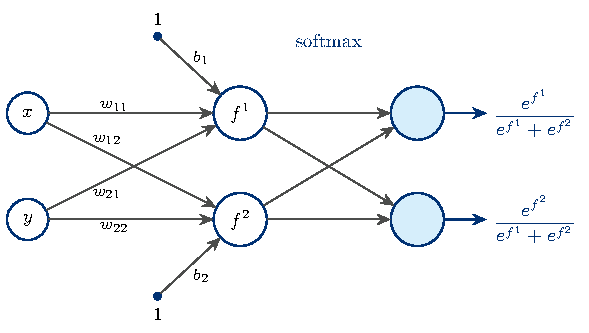
\includegraphics[max width=\linewidth]{Fig40.pdf} 
\caption{Red neuronal con una capa extra implementando la función $\softmax$.}
\label{fig40}
\end{figure}

Este test se puede realizar, por ejemplo, usando la coordenada $z_1$, se tiene
\begin{itemize}
\item Si $z_1>\tfrac12$, entonces $(x, y)\in \G$;
\item Si $z_1<\tfrac12$, entonces $(x, y)\in\bar\G$.
\end{itemize}

El uso de $\softmax$ sirve también para problemas de clasificación que involucran más de 2 clusters. Por ejemplo, en el caso de 3 clusters, $\G_1$, $\G_2$ y $\G_3$, se asocian las etiquetas $\ab_1 = (1,0,0)$, $\ab_2 = (0,1,0)$ y $\ab_3 = (0,0,1)$ que forman un triángulo equilátero en $\R^3$ (el simplex de dimensión $2$). Ver Figura \ref{fig41}. En este caso, el punto de separación se cambia por un sistema de curvas de separación. Ver Figura \ref{fig42}.

\begin{figure}[htbp]
\centering
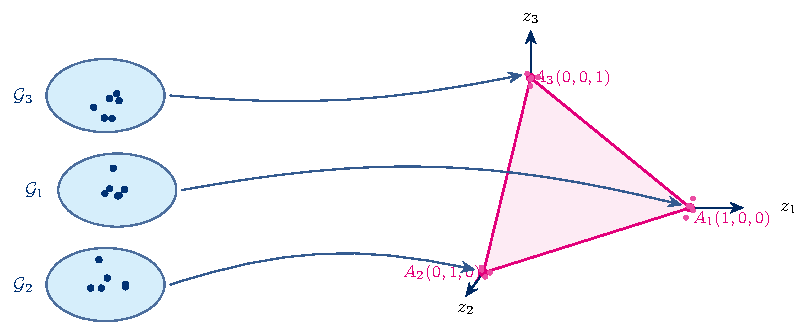
\includegraphics[max width=\linewidth]{Fig41.pdf} 
\caption{Los clusters $\G_1$, $\G_2$, $\G_3$ separables linealmente son mapeados en los vértices de una región triangular.}
\label{fig41}
\end{figure}

Para decidir a qué región de decisión pertenece un punto determinado, se calcula la salida $\zz=\softmax(f(\xx))\in\R^3$ y se elige la coordenada mayor: $\xx$ se asigna a $\G_i$ si $z_i=\max_kz_k$ (equivalentemente, si $f^i(\xx)=\max_kf^k(\xx)$). Las regiones de decisión son las tres regiones del triángulo que se ven en la Figura \ref{fig42}.

\begin{figure}[htbp]
\centering
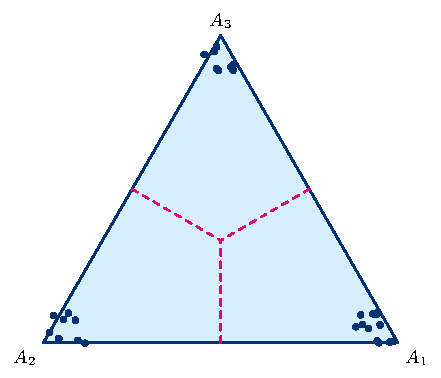
\includegraphics[max width=\linewidth]{Fig42.pdf} 
\caption{Las líneas punteadas separan al triángulo en tres regiones de decisión.}
\label{fig42}
\end{figure}

\subsection{Mapas de decisión no lineales}
Como en el inicio de la sección anterior, consideremos dos clusters en $\R^2$,
$$
\G = \{(x_1,y_1),\dots,(x_N, y_N)\} \quad \text{y}\quad \bar\G = \{(\bar x_1,\bar y_1),\dots,(\bar x_M, \bar y_M)\},
$$
y asumamos que $\hull(\G)\cap\hull(\bar\G)\neq\emptyset$ (por ejemplo, el problema {\em XOR}: $\G=\{(0,0),(1,1)\}$ y $\bar\G=\{(0,1),(1,0)\}$, cuyas cápsulas convexas se cortan en $(\tfrac12,\tfrac12)$).

Asociamos a cada cluster dos números reales $\alpha$ y $\bar\alpha$ respectivamente. Como los clusters no son linealmente separables, buscamos una función no lineal $f\colon \R^2\to\R$ que mapee el cluster $\G$ a un entorno de $\alpha$ y al cluster $\bar\G$ a un entorno de $\bar\alpha$.

\subsubsection*{La neurona sigmoide} El caso más simple de una función no lineal es producido por una neurona sigmoide, con función de entrada-salida dada por
$$
f(x, y) = f_{\ww, b}(x, y) = \sigma(w_1 x + w_2 y + b), 
$$
donde $\sigma(x)$ es la función logística, $\sigma(x) = (1+e^{-x})^{-1}$ (ver Figura \ref{fig43}). Asumamos que las etiquetas se eligen de forma tal que $\alpha=0$ y $\bar\alpha=1$, luego el cluster $\G$ se debe mapear cerca de 0 y el cluster $\bar\G$ cerca de 1.

Observemos que el borde de decisión $\{\sigma(w_1x+w_2y+b)=\tfrac12\}=\{w_1x+w_2y+b=0\}$ sigue siendo una recta. Por lo tanto, una neurona sigmoide {\em no puede} clasificar clusters cuyas cápsulas convexas se intersecan (como en XOR); para eso hace falta una capa oculta, que veremos más abajo. La ventaja de la neurona sigmoide frente al mapa lineal es que satura: los puntos lejanos a la frontera no distorsionan el ajuste como en la Observación anterior. Lo que sigue vale entonces para clusters linealmente separables.

\begin{figure}[htbp]
\centering
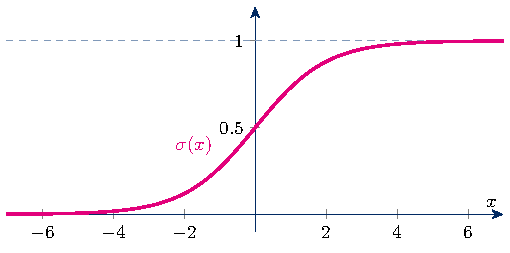
\includegraphics[max width=\linewidth]{Fig43.pdf} 
\caption{La función logística $\sigma(x)$.}
\label{fig43}
\end{figure}

Para que este mapa localice lo mejor posible, necesitamos minimizar la función de costo
$$
F(\ww, b) = \frac12 \sum_{i=1}^N \sigma(w_1 x_i + w_2 y_i + b)^2 + \frac12 \sum_{j=1}^M (\sigma(w_1 \bar x_j + w_2 \bar y_j + b)-1)^2.
$$
Usando la propiedad de la función logística, $\sigma' = \sigma(1-\sigma)$, obtenemos
\begin{align*}
\partial_{w_1} F &= \sum_{i=1}^N x_i \sigma^2(1-\sigma)|_{w_1 x_i + w_2 y_i + b} - \sum_{j=1}^M \bar x_j \sigma(1-\sigma)^2|_{w_1 \bar x_j + w_2 \bar y_j + b}\\
\partial_{w_2} F &= \sum_{i=1}^N y_i \sigma^2(1-\sigma)|_{w_1 x_i + w_2 y_i + b} - \sum_{j=1}^M \bar y_j \sigma(1-\sigma)^2|_{w_1 \bar x_j + w_2 \bar y_j + b}\\
\partial_b F &= \sum_{i=1}^N  \sigma^2(1-\sigma)|_{w_1 x_i + w_2 y_i + b} - \sum_{j=1}^M  \sigma(1-\sigma)^2|_{w_1 \bar x_j + w_2 \bar y_j + b}.
\end{align*}
Este es un sistema no lineal y no se tiene una forma cerrada para la solución del mismo. La forma de encontrar el mínimo entonces es aplicando el método de descenso de gradiente. La sucesión aproximante es dada de forma iterativa por
\begin{align*}
w_1^{(n+1)} &= w_1^{(n)} - \eta \partial_{w_1} F(w_1^{(n)}, w_2^{(n)}, b^{(n)})\\
w_2^{(n+1)} &= w_2^{(n)} - \eta \partial_{w_2} F(w_1^{(n)}, w_2^{(n)}, b^{(n)})\\
b^{(n+1)} &= b^{(n)} - \eta \partial_b F(w_1^{(n)}, w_2^{(n)}, b^{(n)}),
\end{align*}
donde $\eta>0$ es la tasa de aprendizaje. Como valores iniciales se pueden tomar $w_1^{(0)} = w_2^{(0)} = b^{(0)}=0$ (para una única neurona esto es razonable; en una capa oculta, en cambio, la inicialización idéntica de las neuronas no rompe la simetría, ver el Capítulo~\ref{cap6}). Notemos que, con el costo cuadrático, los factores $\sigma(1-\sigma)$ hacen que el gradiente casi se anule cuando la neurona está saturada y equivocada; con la entropía cruzada el gradiente respecto de los parámetros es $(\sigma-z)\,(x,y,1)$ y no tiene ese problema.

Para más de dos clusters se usan etiquetas one-hot y la función softmax, como en la subsección anterior.

\subsubsection*{Una red con una capa escondida} Asumamos que la función no lineal $f$ es el mapa de entrada-salida de una red neuronal feedforward con tres capas, que tiene una salida unidimensional y una capa oculta. Las neuronas en la capa oculta poseen una función de activación no lineal. Entonces el mapa resulta
$$
f(x, y) = f_{W,\lambda, b}(x, y) = \sum_{k=1}^K \lambda_k\sigma(w_{1k} x + w_{2k}y + b_k),
$$
donde $K$ es el número de neuronas en la capa oculta, $w_{ij}$ son los pesos de la entrada en la capa oculta, $b_k$ los sesgos de estas neuronas, y $\lambda_k$ son los pesos de la capa oculta hacia la capa de salida, Ver la Figura \ref{fig44}. La función $f_{W, \lambda, b}$ depende de $4K$ parámetros ($2K$ pesos $w_{ij}$, $K$ sesgos $b_k$, y $K$ pesos $\lambda_k$). 

\begin{figure}[htbp]
\centering
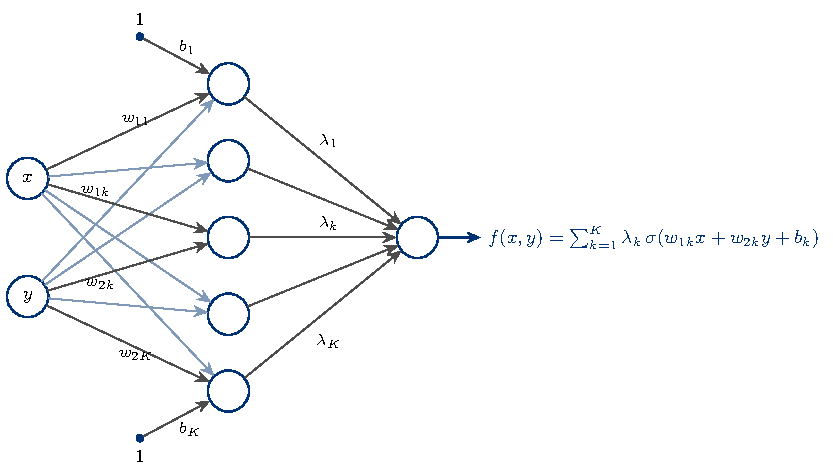
\includegraphics[max width=\linewidth]{Fig44.pdf} 
\caption{Una red neuronal con una capa oculta y salida unidimensional.}
\label{fig44}
\end{figure}

Los parámetros deben ser ajustados de forma de minimizar la función de costo
\begin{equation}\label{18.8.2}
G(W, b, \lambda) = \frac12 \sum_{i=1}^N (f_{W, \lambda, b}(x_i, y_i)-\alpha)^2 + \frac12 \sum_{j=1}^M (f_{W, \lambda, b}(\bar x_j, \bar y_j)-\bar \alpha)^2,
\end{equation}
donde $\alpha$ y $\bar\alpha$ son las etiquetas asociadas con $\G$ y $\bar\G$ respectivamente.

Por el Teorema de Cybenko, como existe una función continua que vale $\alpha$ en $\G$ y $\bar\alpha$ en $\bar\G$ (los clusters son finitos y disjuntos) y una red con una capa oculta puede aproximarla uniformemente, el costo $G$ puede hacerse tan pequeño como se quiera tomando $K$ suficientemente grande, aun cuando los clusters no sean linealmente separables. Es un resultado de existencia: no se tiene una forma cerrada para el minimizante de $G$, que es no convexa, por lo que se necesita aplicar un método de descenso de gradiente, que puede quedar atrapado en mínimos locales. Ver el Ejercicio \ref{18.11.10}.

En el caso de más de dos clusters es conveniente el uso de vectores one-hot como etiquetas. En este caso el espacio de etiquetas es $\R^p$, donde $p$ es el número de clusters que necesitan ser clasificados. Ver el Ejercicio \ref{18.11.11}.

%\section{Bordes de decisión}
%
%Consideremos dos clusters $\G_1$ y $\G_2$ en $\R^2$. Un {\em borde de decisión} es una curva continua en $\R^2$ que separa los clusters. Ver Figura \ref{fig45}. Esto significa que para todo $g_1\in\G_1$ y $g_2\in\G_2$, toda curva continua que une $g_1$ con $g_2$ tiene que intersectar a la curva de borde de decisión.
%
%\begin{figure}
%\label{fig45}
%\includegraphics[max width=\linewidth]{Fig45.pdf} 
%\caption{Borde de decisión entre dos clusters de $\R^2$.}
%\end{figure}
%

\section{Resumen}\label{sec.c10.9}
Durante el proceso de clasificación de los clusters, las etiquetas deben asignarse con precisión a cada uno. Existen varios tipos de etiquetas que pueden utilizarse: números, vectores one-hot, puntos, etc. La función que asigna etiquetas a los clusters se denomina mapa de decisión, y puede ser aprendida por redes neuronales.

Dos clusters finitos son linealmente separables si y sólo si sus cápsulas convexas son disjuntas. En este caso, un perceptrón puede clasificarlos (el algoritmo del perceptrón converge en un número finito de pasos, por el teorema de Novikoff). El ajuste lineal por mínimos cuadrados a las etiquetas es sencillo de resolver, pero no garantiza una buena clasificación.

Si las cápsulas convexas de dos clusters no son disjuntas, entonces no son linealmente separables, y en este caso se requiere una red neuronal con al menos una capa oculta de activación no lineal para aprender la función de decisión correspondiente.

El uso de la función de activación softmax en la última capa de una red neuronal produce vectores de probabilidad, que pertenecen al simplex abierto de dimensión $(n-1)$ cuando hay $n$ clusters; los vértices de ese simplex (los vectores one-hot) son las etiquetas ideales, pero nunca se alcanzan. Los resultados de este capítulo son de existencia: no tratan la generalización a datos nuevos ni el margen entre clusters.

\section{Ejercicios}\label{sec.c10.10}

\begin{ejer}
Sea $\Omega=I_1=[0,1]$ y sea $S = (I_1 \times I_1) \cap (\Q \times \Q)\subset\Omega\times\Omega$ el conjunto de los pares con ambas coordenadas racionales.
\begin{itemize}
\item[(a)] Demuestre que $S$ es una relación transitiva.
\item[(b)] ¿Es $S$ una relación de equivalencia?
\end{itemize}
\end{ejer}

\begin{ejer} \label{18.11.3}
Demuestre que $k$ puntos de $\R^k$ son afínmente independientes si y solo si existe un único hiperplano de dimensión $(k-1)$ que los contiene.
\end{ejer}

\begin{ejer}
Sean $P_1, \dots, P_k$ $k$ puntos afínmente independientes en $\R^k$, y sea $\Hc=\Sb+\pp$ el único hiperplano de dimensión $(k-1)$ que los contiene. Demuestre que el conjunto $\{ P_2-P_1, \dots, P_k-P_1\}$ forma un sistema de vectores independientes en $\R^k$ que genera $\Sb$.
\end{ejer}

\begin{ejer}
Considere dos números reales distintos $x_1, x_2 \in \R$. Demuestre que existe una única función afín $f(x) = ax + b$ tal que $f(x_1) = 1$ y $f(x_2) = 2$.
\end{ejer}

\begin{ejer} \label{18.11.5}
Sea $\G$ un cluster en $\R^n$.
\begin{itemize}
\item[(a)] Demuestre que $\hull(\G)$ es un conjunto convexo.
\item[(b)] Pruebe que $\hull(\G)$ es el conjunto convexo más pequeño en $\R^n$ que contiene a $\G$.
\item[(c)] Demuestre la Proposición \ref{prop1053}.
\end{itemize}
\end{ejer}

\begin{ejer}
Sea $\Phi\colon \R^2 \to \R^2$ una función afín no degenerada, es decir, $\Phi(\xx) = W\xx + \bb$ con $\det W \neq 0$. Considere dos clusters linealmente separables en $\R^2$, $\G_1$ y $\G_2$. Demuestre que $\Phi(\G_1)$ y $\Phi(\G_2)$ son linealmente separables. En otras palabras, las funciones afines preservan la separabilidad lineal.
\end{ejer}

\begin{ejer}
Sea $\G$ un cluster finito de puntos y denote por $g$ su centro de gravedad. Demuestre que $g \in \hull(\G)$.
\end{ejer}

\begin{ejer}
Demuestre que si una familia de clusters $\Gk = \{\G_1, \dots, \G_k\}$ en $\R^n$ es convexamente separable, entonces es mutuamente convexamente separable, es decir, cualquier par de clusters $\G_i$ y $\G_j$ son convexamente separables para todo $i \neq j$. Muestre con el ejemplo de la Observación de la Sección~\ref{sec.c10.5} que la recíproca es falsa si $k\ge3$.
\end{ejer}

\begin{ejer}\label{18.11.9}
\begin{itemize}
\item[(a)] Si $A$ y $B$ son dos conjuntos convexos, compactos y disjuntos, entonces existe un hiperplano que los separa estrictamente. (Mostrar que la hipótesis de compacidad no puede reemplazarse por cerrados: $A=\{(x,y)\colon x>0,\ y\ge1/x\}$ y $B=\{(x,y)\colon y\le0\}$ son cerrados, convexos y disjuntos, pero no están separados estrictamente.)
\item[(b)] Si $\G_1$ y $\G_2$ son dos clusters tales que $\hull(\G_1) \cap \hull(\G_2) = \emptyset$, entonces $\G_1$ y $\G_2$ son linealmente separables.
\end{itemize}
\end{ejer}

\begin{ejer}\label{18.11.10}
\begin{itemize}
\item[(a)] Encuentre el gradiente $\nabla_{W,b,\lambda} G$, donde $G$ está dado por \eqref{18.8.2}.
\item[(b)] Escriba la recursión del descenso de gradiente para la secuencia de aproximaciones del mínimo.
\end{itemize}
\end{ejer}

\begin{ejer}\label{18.11.11}
Considere $p$ clusters, $\G_1, \dots, \G_p$, de puntos en $\R^2$. Escriba la función de costo que asocia el vector $\ee_j$ como etiqueta para el cluster $\G_j$, para todo $j = 1, \dots, p$.
\end{ejer}


\bibliography{biblio}
\bibliographystyle{amsplain}
\end{document}
